\documentclass[b5paper,10pt,twoside]{phdthesis}
\usepackage[total={5in, 7in}]{geometry}
\usepackage{epigraph}
\usepackage{fancyhdr}
\usepackage{multirow}
\usepackage{multicol}
\usepackage{amsmath}
\usepackage{amssymb}
\usepackage{hyperref}
\usepackage{acronym}
\usepackage[table,dvipsnames,svgnames,x11names]{xcolor}
\usepackage[english, dutch]{babel}
\usepackage{booktabs}
\usepackage{array}
\usepackage{url}
\usepackage{rotating}
\usepackage{pxfonts}
\usepackage{pifont}
\newcommand{\cmark}{\ding{51}}%
\newcommand{\xmark}{\ding{55}}%
\usepackage{lettrine}
\usepackage{enumitem}
\newlist{inlinelist}{enumerate*}{1}
\setlist[inlinelist]{label=(\alph*)}
\usepackage{caption}
\usepackage{subcaption}
\usepackage{makecell}
\usepackage[nomessages]{fp}
\newcommand{\maxnum}{100.00} % bar inside table cell
\newlength{\maxlen}
\newcommand{\databar}[2][green!25]{%
  \settowidth{\maxlen}{\maxnum}%
  \addtolength{\maxlen}{\tabcolsep}%
  \FPeval\result{round(#2/\maxnum:4)}%
  \rlap{\color{green!25}\hspace*{-.5\tabcolsep}\rule[-.05\ht\strutbox]{\result\maxlen}{.95\ht\strutbox}}%
  \makebox[\dimexpr\maxlen-\tabcolsep][r]{#2}%
}

% Epigraph config
\setlength{\epigraphwidth}{25em}
\setlength{\epigraphrule}{0pt}

\makeatletter
\g@addto@macro{\UrlBreaks}{\UrlOrds}

%   Parameters for TEXT pages (not float pages):
\setcounter{topnumber}{2}
\setcounter{bottomnumber}{2}
\setcounter{totalnumber}{4}     % 2 may work better
\setcounter{dbltopnumber}{2}    % for 2-column pages
\renewcommand{\dbltopfraction}{0.9}	% fit big float above 2-col. text
\renewcommand{\textfraction}{0.07}	% allow minimal text w. figs
%   Parameters for FLOAT pages (not text pages):
\renewcommand{\floatpagefraction}{0.7}	% require fuller float pages
% N.B.: floatpagefraction MUST be less than topfraction !!
\renewcommand{\dblfloatpagefraction}{0.7}	% require fuller float pages

\makeatletter
\newcommand*{\rom}[1]{\expandafter\@slowromancap\romannumeral #1@}
\makeatother

\DeclareSymbolFont{extraup}{U}{zavm}{m}{n}
\DeclareMathSymbol{\varheart}{\mathalpha}{extraup}{86}
\DeclareMathSymbol{\vardiamond}{\mathalpha}{extraup}{87}

\makeatletter
\def\zaptype#1{%
\listsubcaptions % Finish the last set of sub-floats before
\def\@captype{#1}}% switching to another float type.
\makeatother

\graphicspath{{./Figures/}}

\newcolumntype{C}[1]{>{\centering\let\newline\\\arraybackslash\hspace{0pt}}m{#1}}


\newcommand{\abstract}{%
   \chapter*{Abstract}%
   \addcontentsline{toc}{chapter}{Abstract}%
   \markboth{Abstract}{Abstract}%
}


\newenvironment{Abstract}
{\begin{center}\textbf{Abstract}
 \end{center} \small \begin{quote}}
{\end{quote}}

\pdfcompresslevel=0

\begin{document}
%\thispagestyle{empty}

%%\begin{figure}
%	\vspace*{-1.15in}
%	\hspace*{-0.825in}
%	\includegraphics[width=17cm,height=24cm]{CoverPage}
%\end{figure}
COVER
%\cleardoublepage

\sloppy
\pagestyle{empty}
\thispagestyle{empty}
\newgeometry{bottom=0.5cm}
\large
\vspace*{-3cm}

\hspace*{-0.5cm}
\includegraphics[width=7.38cm]{Figures/rugr_logoen_zwart_rgb.jpg}

\begin{center}

\vspace{1cm}

{\fontsize{25pt}{30pt}\selectfont \textbf{Managing technical debt:}\\\textbf{prioritising and quantifying architectural smells}}


\vspace{2.5cm}

\textbf{\Large{PhD thesis}}

\vspace{1.6cm}
% \vfill\vfill\vfill\vfill

to obtain the degree of PhD at the\\
University of Groningen\\
on the authority of the\\
Rector Magnificus Prof.\ C.~Wijmenga\\
and in accordance with\\
the decision by the College of Deans.

\vspace{0.4cm}

This thesis will be defended in public on

\vspace{0.4cm}

19 December 2022

\vspace{1cm}

by

\vspace{1cm}

\textbf{\Large{Darius Sas}}\\

\vspace{0.4cm}

born on 16 December 1992\\
in Turda, Romania
\end{center}
\enlargethispage{\baselineskip}

\restoregeometry
\clearpage
\thispagestyle{empty}
\noindent
\\
\textbf{Supervisor}\\
Prof.\ P.\ Avgeriou\\

\noindent
\\
\textbf{Co-supervisor}\\
Prof.\ F.\ Arcelli Fontana\\

\noindent
\\
\textbf{Assessment committee}\\
Prof. A. Capiluppi\\
Prof. S. Demeyer\\
Prof. G. Robles\\

\vfill
\normalsize

\thispagestyle{empty}
\noindent

The research reported in this thesis has been conducted in the Software Engineering and Architecture group of the Bernoulli Institute for Mathematics, Computer Science and Artificial Intelligence of the University of Groningen, The Netherlands. 

\vfill\vfill\vfill

% \noindent
% Cover details: The geometric forms on the front and back side of the cover refer to two different implementations of similar features of a robotic face. This is an analogy to the possibility of having different instantiations of one same design pattern, which may express different levels of one or more quality attributes. The curve delineated by a dark shade of red is an analogy to measurements quality levels in a time series. Finally, the font used in the cover is named \textit{Roboto}, by Christian Robertson. 

\vspace*{\fill}

% TODO change title
\noindent Technical Debt Repayment in Practice\\
\noindent Darius Sas\\

\normalsize
\newpage
%\include{0.assessment-committee}
\pagenumbering{gobble}% Remove page numbers (and reset to 1)

\null
\thispagestyle{empty}%
\addtocounter{page}{-1}%
\newpage

\clearpage
\thispagestyle{empty}
\newpage

\vspace*{7cm}

\begin{center}
\large{To my parents and brother.} \\
\end{center}

%\newpage

\pagenumbering{gobble}% Remove page numbers (and reset to 1)

\null
\thispagestyle{empty}%
\addtocounter{page}{-1}%
\newpage

\begin{abstract}
    Introduction to technical debt....

    Architectural smells refer to violations of well known design principles that result in undesired dependencies, overblown size, and excessive coupling.
    Architectural smells have a negative influence on the maintainability levels of the system, making it harder to apply changes and add new functionality.
    Researchers have identified, described, and categorised several types of architectural smells over the past years.
    Subsequently, several research tools were born to automatically detect such smells starting from the source artefacts of a system.


    From a practical point of view, in order to properly be able to manage the technical debt generated by architectural smells, identification alone is not enough.
    To properly address the threat posed by architectural smells to the maintainbility of a system, practitioners require support for the prioritisation, quantification, and monitoring activities as well.
    Unfortunately, the literature on the topic is incomplete, and the tool support for these specific activities is missing.
    \textbf{This thesis reports reports on the investigation of how practitioners manage architectural smells in practice, what strategies exist to prioritise architectural smells refactoring, and design a methodology to quantify and monitor their contribution to technical debt.}

    There exist several types of architectural smells, therefore, to narrow down the scope of the investigation, we decide to focus on the four types that are the most prominent in the literature: Cyclic Dependency (CD), Hublike Dependency (HL), Unstable Dependency (UD), and God Component (GC).
    
    To address the problem stated above, we first opted to analyse the evolution of individual architectural smell instances in long-lived, open source systems by mining their software repositories.
    This allowed us to investigate prioritisation opportunities based on the history of an architectural smells.
    The results show how different smell types differ in multiple aspects, such as their growth rate, the importance of the affected elements over time in the dependency network of the system, and the time each instance affects the system.
    Based on these differences, we extrapolated that the refactoring of HL smells should be prioritised over CD smells and that many CD instances should have a low priority as they are likely to be organically removed in the upcoming releases.

    %Another finding of this study was that some of the smells are the result of intentional design decisions.
    These findings however are based on the mining software repositories, thus they can only tell half the story.
    Therefore, we decided to ask 21 software practitioners their opinion on architectural smells and what smells they think are more disruptive for the maintainability of a system.
    The findings show that practitioners think of certain smells as more impacful than others.
    One above all is the GC smell, that is perceived more detrimental the others, although the opinion on the HL smell was quite similar.
    These findings match the findings of the previous study.
   
    Another finding is that practitioners are aware of the smells, but they struggle to diligently implement good design practices with the resources (money and time) available to them.
    This motivated us to further investigate how architectural smells are introduced, and to broaden the scope, also how they co-occur, and evolve over time in an undustrial context.
    We set up an industrial case study to investigate these aspects in the context of large multinational company that works in C/C++, and verify whether the findings of the previous studies (that were all based on Java systems) apply to this context as well.
    The findings showed that CD smells, although they are not very persistent within the system, are precursors to other smell types.
    Therefore, CD instances can be used as a red flag that notifies practitioners that a component might arise a more severe architectural smell soon. Indeed, 94\% of HL smells, were also part of a cycle.
    
    The study also elicitated the opinion of software engineers and architects, who mentioned that the most problematic aspect of architectural smells are change ripple effects, that are unpredictable.
    This motivited us to investigate the relation between architectural smells and source code changes.
    After analysing over 30 open source Java systems, we ran a series of statistical tests to determine whether source code changes were more frequent, and larger in size, in components that were affected by smells than in non-smelly components.
    The findings show that this is indeed the case, and that all four architectural smells correlate with higher frequency of change of the affected part. 
    Interestingly, after talking to practitioners in the previous study we expected UD to be the smell with the highest correlation with changes. THis turned out, however, not to be the case as the HL smell beat UD by over 10\%.
    This means prioritising the refactoring of HL instances over the other smell types is a more advantageous approach for practitioners.

    The answers collected up until this point provide valuable insights on how architectural smells are preceived by practitioners, how they get introduced, how they co-occur, and how they correlate with the changes done in the system.
    These findings allowed us to extrapolate valuable information on what are the best strategies to prioritise smell instances and what makes one instance more severe than the other.
    Therefore, using the acquired knowledge, we created a machine learning model that ranks architectural smells based on their severity that performs rather well (97\% of instances are ranked above a less severe smell).
    This model makes it easier for practitioners to prioritise architectural smells, especially in very large systems where hundreds of instances can be detected.
    Additionally, using this model, we designed an approach to quantify the amount of technical debt generated by the architectural smells detected in a system.
    The validation of the model showed that in 71\% of the cases, practitioners agreed that the estimations provided were representative of the effort necessary to refactor the smell.


    %Copy abstract of previous papers



\end{abstract}

%Enabling technical debt repayment for architectural smells

\selectlanguage{dutch}

\samenvatting{Technical Debt (Technische schuld-TD) is een metafoor ...}

\cleardoublepage

\selectlanguage{english}

\clearpage
\lhead[]{\fancyplain{}{\rightmark}}
\chead[\fancyplain{}{}]{\fancyplain{}{}}
\rhead[\fancyplain{}{\leftmark}]{\fancyplain{}{}}

\begingroup
	\pagestyle{fancyplain}
	\pagenumbering{roman}
	\let\cleardoublepage\relax
	\let\clearpage\relax
	\tableofcontents
%	\setlength{\cftparskip}{-0.0775\baselineskip}
	\newpage
	\cleardoublepage
	\phantomsection
	\addcontentsline{toc}{chapter}{List of Figures}
	\listoffigures
	\newpage
	\cleardoublepage
	\phantomsection
	\addcontentsline{toc}{chapter}{List of Tables}
	\listoftables
\endgroup

\pagestyle{plain}
\cleardoublepage
\phantomsection
\addcontentsline{toc}{chapter}{Acknowledgements}
\chapter*{Acknowledgements}

When I started my PhD in 2018 some of the other PhD students were finishing theirs.
This gave me the opportunity to go through their dissertations and get a sneak peek of what was expected of me.
As one could imagine, their work was outstanding and, most impressively, of the highest scientific standard.
Immediately, I thought to myself that I would never be able to achieve something like that.

After four years I can say for certain that I was indeed right, I could never finish this journey -- not alone!
Therefore, I would like to spend the next few paragraphs expressing my most sincere gratitude to all the people who supported me.

First and foremost, I would like to thank my two supervisors, Prof. Paris Avgeriou and Prof. Francesca Arcelli.
Dear Paris, I could not ask for a better supervisor and mentor. Your way of thinking and approaching science has helped me not only become a better researcher but also a better person. 
Your encouragement and guidance helped me overcome obstacles I deemed insurmountable.
I wish I could be half as good of a scientist as you are, but I will be happy even being half as good as you think of me. Thank you.

Dear Francesca, you always believed in me and were always there to help whenever I needed a hand. This holds not only for my PhD but also for my MSc and BSc theses.
You always believed in me and encouraged me to do more and better. I want to deeply thank you for your mentorship and all the opportunities you gave me. I wouldn't have done this without you.

I would like to sincerely thank the assessment committee, Prof. Andrea Capiluppi, Prof. Serge Demeyer, and Prof. Gregorio Robles, for taking the time to read my thesis and providing me with valuable feedback.

I am also grateful to my brother, Cezar Sas. Cezar, I deeply appreciate that we managed to travel, explore, bike, hike, chat and cook together over the past years. I genuinely treasure these moments and I hope we can share many more in the upcoming years! 

I would also like to thank Jie Tan. Dear Jie, we started our PhD journey together, and, as you would like to jokingly point out, you finished much earlier than me! To be honest, I never stood a chance against you! 
Seeing your commitment and sheer will facing setbacks was inspiring and helped me endure mine.
I am glad we sailed together the sea of adversities entailed by a PhD, and I want you to know that I hold dear to the lifelong memories of our wonderful travels, food, and wine we shared.

Another person I must absolutely thank is Francesco Olivari. Dear Francesco, you are one of the most sincere and genuine people I know.  
I wish we could meet and share a burger -- rigorously at Wereldburgers -- like we used to do during our time in Groningen.
Thank you for hanging out with me! 

Dear Ilaria, I am so grateful we shared the same research interests and got the chance to work on the same research topic as you. I am sure that our future professional endeavours will be more than successful!

Dear Andrea, Yuri, and Ottavio. You are my lifelong friends, and I am so grateful for your support throughout these years. 
After four years spent abroad, I cannot wait to get the chance to hang out with you and watch (and discuss) movies, music, and video games!

Dear Simone, Marco C., Matteo, Marco G., Kristina, Susanna, and Marco De G., thank you for the amazing time we spent together. It is always nice joining you for dinner and other social activities!

Dear Bozhidar, you have no clue how much you helped me throughout this PhD. You cheered me up during my lows and helped me look forward with a positive mindset.

Naturally, I must also express my gratitude to the people at the Software Engineering group (SEARCH) of the Bernoulli Institute that I have not mentioned earlier: Dr. Vasilios Andrikopoulos,  Dr. Ayushi Rastogi, Dr. Daniel Feitosa,  Dr. Mohamed Soliman, H\'ector Cadavid, Ruiyin Li, Yikun Li, João Biazotto, Zaki Pauzi, Sara Mahdavi-Hezavehi, and Anja Reuter. 
I am honoured I worked with you, and that, every so often, shared a beer with you!

Last but not least, I wish to state my utmost appreciation to my parents.
Their unconditional support and sacrifice are what made me the person I am today.


\begin{flushright}
    Darius Sas\\
    Rome\\
    August 22, 2022
\end{flushright}

\clearpage

\pagestyle{headings}
\newcommand{\publ}{}

\pagestyle{fancyplain}
\renewcommand{\sectionmark}[1]{\markright{\it \thesection.\ #1}}
\renewcommand{\chaptermark}[1]{\markboth{
       \it \thechapter.\ #1}{}}
\lhead[\thepage]{\fancyplain{}{\rightmark}}%\publ
\chead[\fancyplain{}{}]{\fancyplain{}{}}
\rhead[\fancyplain{}{\leftmark}]{\fancyplain{}{\thepage}}
\lfoot[]{}
\cfoot[]{}
\rfoot[]{}
%------------------------------

\pagenumbering{arabic}
\setcounter{page}{0}

%Intro
\chapter{Introduction}\label{chap:introduction}

\epigraph{\emph{A program that is used and that, as an implementation of its specification, reflects some other reality, undergoes continuous change or becomes progressively less useful.
The change or decay process continues until it is judged more cost effective to replace the program with a recreated version.}}{--- Meir Lehman}

%\section{The relentless endeavor of software craftmanship}
\lettrine{T}{he} opening quote of this chapter is the first of the five laws of software evolution formulated by Lehman in the late 1970's \cite{Lehman1979}.
The law refers to the fact that all software is designed to operate in a specific environment and to satisfy a specific set of requirements. 
However, every environment, and every requirement, is bound to change eventually, rendering the software obsolete. %, unless it changes accordingly.
Therefore, the need of constantly adapting a software to new requirements, and shifts in the environment, is a \emph{relentless endeavor} that, over time, destabilises the sustainability of a software project.

A software project is \emph{sustainable} if the project owner is capable of applying whatever valuable change they ought to make, timely \cite{Winters2020}.
However, decisions and implementation choices made early on in the project's lifetime inevitably affect the decisions we have to make in the present, often making them harder.
Over time, as the system grows old, our capability of adapting the software to new requirements and changes in the environment grows narrower, and making changes becomes more expensive.
Eventually, the system becomes \emph{unsustainable} and the second part of Lehman's first law of software evolution comes into play.
In other words, a system that is unsustainable is a system that is \emph{poorly maintainable} and with \emph{limited capabilities} to evolve. 

In 1992, Ward Cunningham cleverly adapted and reframed these concepts under the term \emph{technical debt} \cite{Cunningham1992}. %TODO: improve this sentence
Since then, technical debt has gained a lot of traction among both practitioners and researchers alike.
Indeed, the presence of technical debt within a system is a problem that every non-trivial software system suffers from, and over the years, several studies have made great progress in identifying the causes and effects of technical debt \cite{Brown2010,Kruchten2012,Lehman1979}.
Technical debt can materialise into various forms, ranging from source code violations \cite{Letouzey2012,Curtis2012} and design level flaws \cite{Marinescu2012} to high-level decisions made at the architectural level \cite{Ernst2015,Yli-Huumo2014}.
In this regard, architectural smells (AS), defined as a \emph{``commonly (although not always intentionally) used architectural decisions that negatively impact system quality} \cite{Garcia2009} have gained a lot of attention from researchers over the past years \cite{Verdecchia2018}.
AS contribute to the degradation of a software project's maintainability, and since they involve high-level artefacts, their impact is mostly perceived on the long term. 
Although existing literature has devoted a considerable amount of effort to study AS \cite{Mo2015,Le2016,Arcelli2016}, our understanding of AS is still incomplete.
This dissertation aims at improving the current state of the art concerning our understanding of AS by answering questions such as: \emph{how are AS introduced?; how do AS evolve?; and, what is their impact on software maintenance (i.e. technical debt)?}

The fundamental proposition of this thesis is that a better understanding of AS will allow software practitioners to better manage technical debt, and therefore defer the second part of Lehman's first law of software evolution.

In the upcoming sections, I will introduce the concepts of technical debt and architectural smells in further detail, as these are the \emph{leitmotif} of this dissertation.
I will also decompose the research problem addressed in this thesis into multiple research questions and explain the methodology used to answer them.


\section{Technical Debt}
In 1992, Cunningham first introduced the concept of \emph{technical debt} (TD) \cite{Cunningham1992}. 
The term was first coined to indicate the necessity of releasing software that, while it works perfectly, it does not meet the criteria of long-term sustainable software. 
Cunningham himself calls this an \emph{``unmasterable program''} that is \emph{``dangerous''} unless the \emph{debt} is repaid.
Unfortunately, TD repayment is not always feasible, as software practitioners have to work with limited time and budget, resulting in most of TD not being repaid \cite{Digkas2018}.
The time spent on not-quite-right code counts as \emph{interest} on that debt \cite{Cunningham1992}, making software projects more expensive to maintain.
Technical debt is a powerful metaphor that, essentially, conveys the importance of sustainable software -- and of Lehman's first law of software evolution -- in terms that are easy to understand and communicate to others. 
%Essentially, saying that a system has incurred a lot of technical debt, or that it is unsustainable, is saying that the system is \emph{poorly maintenainable} and with \emph{limited capabilities} to evolve. 

A modern definition of TD is the following: \emph{TD reflects the technical compromises that software practitioners make in order to achieve a short-term advantage at the expense of creating a technical context that increases complexity and cost in the long-term} \cite{Avgeriou2016}. 
Hence, a company can get into debt and, as long as it is aware of the debt and is planning to repay it in the medium-term period, leverage on it to temporarily increase productivity.
However, if the company is not aware that it is accruing TD, or does not repay it on time, the amount of interest may become too high, causing the failure of the project due to the huge cost of implementing changes.

During the course of the years, the metaphor has been extended by the research community and has assumed a wider meaning, engulfing several aspects of the software development process like architecture, design, requirements, testing and documentation \cite{Brown2010}.
The current literature has explored the concept in all of its vastness and has proposed and analyzed multiple taxonomies and types of TD.
A common way of categorising TD is by the type of artefacts it affects. Using this approach, Li et al. \cite{Li2015} identified several different types of TD, namely \emph{Requirements TD}, \emph{Architectural TD}, \emph{Design TD}, \emph{Code TD}, \emph{Test TD}, \emph{Build TD}, \emph{Documentation TD}, \emph{Infrastructure TD}, and \emph{Versioning TD}.

In this thesis, I will mostly focus on \emph{Architectural TD} (ATD), the type of TD that affects the architecture of a software.
Examples of ATD are architectural violations (e.g. the implemented architecture is not compliant with a set of predefined architectural rules), poor application of well-known architectural patterns, early architectural decisions that had unexpected trade-offs, or architectural smells.
This particular type of ATD is going to be, as mentioned earlier, the focus on this dissertation.

\section{Architectural smells}

% \subsection{Why smells over existing metric?}

\section{The project SDK4ED and Arcan}
% Explain how the SDK4ED and Arcan are an important part of the PhD

\section{Research design}
\subsection{Problem statement}
In the early years of the research on architectural smells, researchers focused on identifying new types of smells, theoretically define them, propose a detection rule, and finally describe their impact on software maintenance from a theoretical point of view \cite{Lippert2006,Garcia2009,Mo2015,Le2016,Arcelli2016}.
From there, researchers moved on to study how smells impact software maintenance in open source systems \cite{Choudhary2016,Xiao2016,Le2018}, study their interaction with other types of smells \cite{Sharma2017,Arcelli2019}, and even predict their introduction in future releases \cite{Arcelli2019b}.
All of these studies offer a great insight into the theoretical nature of architectural smells, and some of them even provide limited evidence to support whether the hypothesized negative effects on software maintenance are detectable in real world systems.
However, there are still three important research threads that are either incomplete or not investigated at all:
\begin{enumerate}
    \item there are no specific details on how individual architectural smell instances evolve over time. This means that it is not clear how architectural smells are \emph{introduced}, how long they \emph{persist} within the system, and whether any TD interest is \emph{paid} on the components affected by architectural smells; 
    
    \item no studies investigate how architectural smells are \emph{perceived} by practitioners. This means that there is little to no empirical evidence on how architectural smells concretely affect the work of software developers and architects;
    
    \item only a few studies investigate the possibility to \emph{estimate} the amount of technical debt principal generated by architectural smells, but these approaches either lack an industrial validation or use limited approaches to estimate it. 
\end{enumerate}
If architectural smells are to be used by practitioners to manage TD, these three research areas are of paramount importance in order to achieve that.
%The lack of research in these three areas severely limits the application of architectural smells in practice.

The three points highlighted above can be summarised under the following problem statement:
\begin{quote}\itshape
    ``Existing literature on architectural smells does not document how AS are introduced, how long they persist, and how software practitioners are impacted by AS. 
    This limits existing implementations of a fully-automated, data-driven approach to manage the technical debt generated by architectural smells.''
\end{quote}

\subsection{Design science as research methodology}
The research project that this dissertation is based on adopts the design science framework developed by Wieringa \cite{Wieringa2014} and depicted in Figure \ref{fig:design-science}.
Design science is the \emph{design} and \emph{investigation} of artefacts (e.g. a software component, a method, a service, an organisation, etc.) in context \cite{Wieringa2014}.
Design, because it allows to design an artefact that improves a problem context, namely, that solves a \emph{design problem}. 
Investigation, because it allows to answer \emph{knowledge questions} about the artefact in context.

Design problems call for a change in the real world; in contrast, knowledge questions ask for knowledge about the real world.
The distinction between design problems and knowledge questions is often confusing, as design problems can be formulated to look like knowledge questions.
Figure \ref{fig:design-science} can help us distinguish these: if the question asks  \emph{about a solution} to a problem, then it is a design problem; if it seeks knowledge \emph{about the world}, then it is a knowledge question.

A concrete example of design science is Software Engineering itself \cite{Wieringa2014}.
Software Engineering is a design science that seeks to understand and solve the problems of creating and maintaining software to achieve the stakeholders' goals.

A concrete example of design problem is: \emph{design an approach to measure technical debt principal generated by architectural smells.}
A concrete example of knowledge question is: \emph{how accurate is such an approach?}.

\begin{figure}
    \centering
    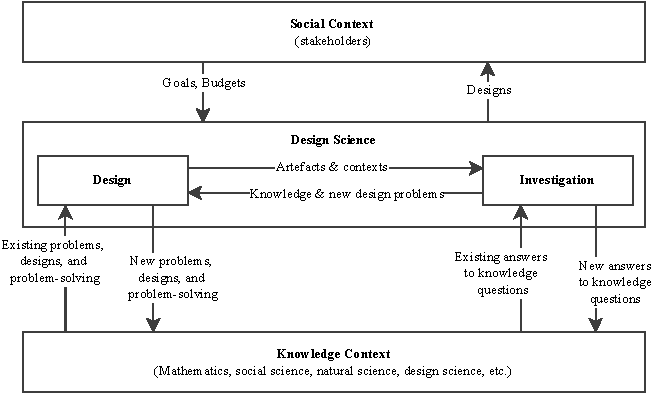
\includegraphics[width=.9\textwidth]{c1/design-science-diagram.pdf}
    \caption{The framework for design science proposed by Wieringa \cite{Wieringa2014}.}\label{fig:design-science}
\end{figure}

To frame the research project presented in this dissertation into the design science framework of Wieringa, w

\subsection{Problem decomposition}
\begin{figure}
    \centering
    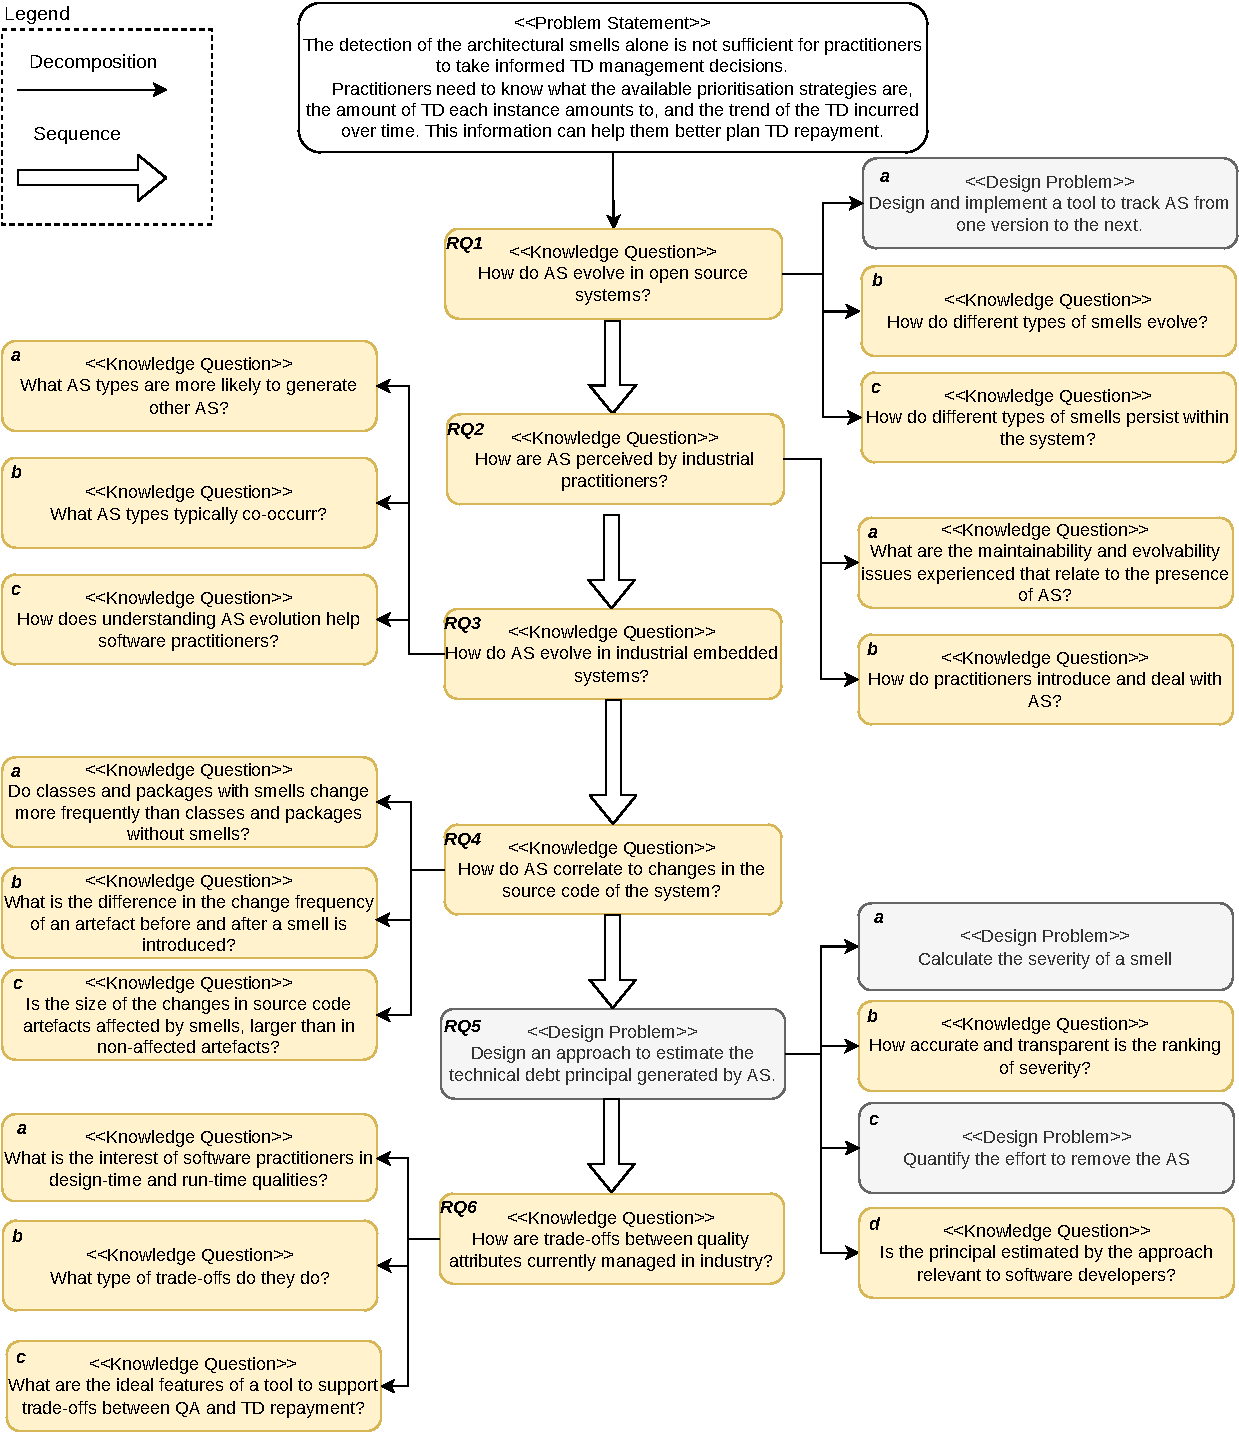
\includegraphics[width=\textwidth]{c1/problem-decomposition.pdf}
    \caption{A caption}\label{fig:problem-decomposition}
\end{figure}
\subsection{Overview of this dissertation}



% % Paper 1 - 
\setlength{\headheight}{1.2cm}
\renewcommand{\publ}{\flushleft\footnotesize{Based on:\\[0.1cm]
		\textit{D. Sas, P. Avgeriou and F. Arcelli Fontana, "Investigating Instability Architectural Smells Evolution: An Exploratory Case Study," 2019 IEEE International Conference on Software Maintenance and Evolution (ICSME), 2019, pp. 557-567, doi: 10.1109/ICSME.2019.00090.} \\[0.1cm]
}}

\chapter{Investigating instability architectural smells evolution: an exploratory case study}\label{chap:2}
\epigraph{\emph{I've learned to always avoid saying ``always''.}}{--- Martin Fowler}


\begin{Abstract}
    Architectural smells may substantially increase maintenance effort and thus require extra attention for potential refactoring. While we currently understand this concept and have identified different types of such smells, we have not yet studied their evolution in depth. This is necessary to inform their prioritisation and refactoring.
    This study analyses the evolution of individual architectural smell \emph{instances} over time, and the \emph{characteristics} that define these instances.
    Three different types of architectural smells are taken into consideration and mined from a total of 524 versions across 14 different projects.
    The results show how different smell types differ in multiple aspects, such as their growth rate, the importance of the affected elements over time in the dependency network of the system, and the time each instance affects the system. They also cast valuable insights on what aspects are the most important to consider during prioritisation and refactoring activities.
\end{Abstract}

\section{Introduction}
In recent years, there has been increasing interest on the concept of \emph{architectural smells} (AS): issues in the architecture that often cause extra maintenance effort \cite{Lippert2006}. Several studies have explored this concept and identified different types of such smells \cite{Lippert2006,Garcia2009,Suryanarayana2014a,Mo2015}.
However, while the evolution of \emph{code} smell instances has been extensively investigated, very few studies focus on the evolution of \emph{architectural} smells and do so only at a coarse-grained level (e.g. by simply counting the number of smells in each version). There is also no work tracking the individual smell instances along system evolution.

We need to study the evolution of AS in detail because AS are a different type of ``affliction" than code smells: they usually involve more elements than code smells, they affect the system at a different scale, and they require more effort to be refactored \cite{Lippert2006}. At the same time,  the long-term advantages of this refactoring in terms of maintainability and changeability of the system are higher. Thus, the current theoretical knowledge on code smells cannot be applied to AS.

In this study, we propose an approach to study the evolution of AS detected by an open source tool named \textsc{Arcan} \cite{Arcelli2017}, by tracking individual smell instances and measuring the evolution of the properties of each detected instance. We have detected almost 150.000 unique smell instances in over 500 versions across 14 open source Java projects.
We have performed four types of analyses: a generic data mining analysis to have a better understanding of the data, a trend analysis to understand the evolution of the smells over time, a correlation analysis to identify possible correlations among the smell characteristics\footnote{See Section \ref{c2:sec:smell-characteristics} for the definition of characteristics and the full list.} considered, and a survival analysis to document their probability to persist within the system.
The focus of this study is on the architectural smells known as instability AS \cite{Arcelli2016}; these are introduced in more depth in Section \ref{c2:sec:arch-smells}.

Our findings can enable practitioners and researchers to develop strategies for optimal refactoring prioritisation of individual smell instances based on multiple factors.
For example, a Hublike dependency smell is a much better option for refactoring than a Cyclic dependency, especially in terms of complexity, and future and present maintenance effort.
Additionally, Cyclic dependencies have a much shorter lifetime on the average, making them less critical in general.

The remainder of this chapter is organised as follows: Section \ref{c2:sec:related-work} discusses similar work in the literature, Section \ref{c2:sec:arch-smells} introduces the smells hereby considered, Section \ref{c2:sec:case-study} explains the methodology of this case study, Sections \ref{c2:sec:general-results}, \ref{c2:sec:rq1a-results}, \ref{c2:sec:rq1b-results}, and \ref{c2:sec:rq2-results} report and discuss the results of the different analyses, Section \ref{c2:sec:threats} lists the threats to the validity of this study and finally Section \ref{c2:sec:conclusions} concludes the chapter.

\section{Related work}\label{c2:sec:related-work}
We present related work concerning both architectural smells and code smells.

In the former case, Al-Mutawa et al. \cite{AlMutawa2014} have investigated the circular (or cyclic) dependencies' shape in Java programs. 
They developed and validated a methodology to detect and classify circular dependencies starting from the bytecode of an application.
Their findings, based on a case study performed on the Qualitas Corpus \cite{QualitasCorpus2010} data set, suggest that the most common shapes (see Figure \ref{c2:fig:cycle-shapes}) are tiny and multi-hub. Moreover, they also argue that cycles among parents and children packages are less critical than cycles among non-related packages, providing empirical evidence to back up their claims.

Another study that considers the history of architectural smells was published by Roveda et al. \cite{Roveda2018}.
In their work, the authors try to estimate the architectural debt index using architectural smells and track the evolution of the index throughout a system's history.
The calculation uses partial historical information of the AS identified by the \textsc{Arcan} tool in multiple versions.
The major shortcomings of Roveda et al.'s index are:
\begin{enumerate}[label=(\roman*)]
    \item the historical information used is limited to the size of the smell and only considers the previous version,
    \item the historical information is weighted equally for every smell type, and
    \item it does not account for the \emph{magnitude} of the variation, i.e. a decrease by only one element halves the contribution of the smell to the overall index, whereas an increase by only one doubles it.
\end{enumerate}
Indeed, one of the goals of this work is also to provide theoretical background and practical tools to improve such types of calculation.

Concerning code smells, there are several works on tracking smells throughout a system's history.
In their work, Vaucher et al. \cite{Vaucher2009} have focused on the code smell God Class and its evolution in terms of the degree of \textit{``godliness"}, estimated using their previous approach based on Bayesian belief networks.
The authors analysed the trend of such a parameter for each God Class instance in the history of two systems. Their findings suggest that the godliness of God classes tends to remain constant in over 60\% of the cases.

A different perspective on code smells evolution was introduced by Chatzigeorgiou et al. \cite{Chatzigeorgiou2014}, who analysed the survival probability of four types of code smells. Their findings show that Long Methods are the most persistent code smells in the two analysed systems.

In a similar work, Peters et al. \cite{Peters2012} have also analysed the persistence of code smells in a system, though they have used a slightly less elaborate technique to do so and on a slightly different set of smells.
Their findings show that Feature Envy methods are the least persistent type of smell (similarly to the finds of Chatzigeorgiou et al.) and that Data Classes are, instead, the most persistent ones.
% Other possible RW: Tsantalis, Olbrich, Tufano

\section{Architectural smells}\label{c2:sec:arch-smells}
\subsection{Definitions and implications}
This section introduces the architectural smells (AS) considered by this dissertation. The definition of these smells is provided by Arcelli et al. \cite{Arcelli2016} and briefly reported here.

\paragraph{Unstable dependency (UD)}\label{c2:sec:arch-smells-ud}
This smell represents a component that depends upon a significant number of components that are less stable than itself.
The stability of a component is measured using Martin's instability metric \cite{Martin2018}, which measures the degree to which a component (e.g. a package) is susceptible to change based on the classes it depends upon and on the classes depending on it.
The smell thus arises when a component has a significant number of components -- the tool \textsc{Arcan} uses a 30\% threshold \cite{Arcelli2017} -- it depends upon with an instability value higher than its own.
A UD smell is detectable on Java package-like elements only (i.e. containers of classes, files, etc.). A simplified example of UD is shown in Figure \ref{c2:fig:ud}. 

The main problem caused by UD is that the probability to change the main component grows higher as the number of unstable components it depends upon grows accordingly. This increases the likelihood that the components that depend upon it (not shown in Figure \ref{c2:fig:ud} for simplicity) change as well when it is changed (ripple effect), thus inflating future maintenance efforts.

\paragraph{Hublike dependency (HL)}\label{c2:sec:arch-smells-hl}
This smell represents a component where the number of ingoing and outgoing dependencies is higher than the median in the system and the absolute difference between these ingoing and outgoing dependencies is less than a quarter of the total number of dependencies of the component \cite{Arcelli2016}. A hublike dependency can be detected both at the package and at the class level.

The implications of this smell for development activities are once again concerning the probability of change and the ease of maintenance. Consider, for example, the case represented in Figure \ref{c2:fig:hl}.
Making a change to any of the components that A depends upon may be very hard \cite{Martin2018}, even though there is only one component depending on them.
Additionally, the central component is also overloaded with responsibility and has a high coupling.
This structure is thus not desirable, as it increases the potential effort necessary to make changes to all of the elements involved in the smell.

\paragraph{Cyclic dependency (CD)}\label{c2:sec:arch-smells-cd}
This smell represents a cycle among a number of components; there are several software design principles that suggest avoiding creating such cycles \cite{Lippert2006,Parnas1979,Stevens1974,Martin2018}.
Cycles may have different topological shapes. Al-Mutawa et al. \cite{AlMutawa2014} have identified 7 of them; the ones detected by \textsc{Arcan} are shown in Figure \ref{c2:fig:cycle-shapes} \cite{Arcelli2017}.
Usually, the circle shape is intuitively perceived as the typical CD (i.e. see Figure \ref{c2:fig:cd}), but it is certainly not the only possible type of CD. In fact, there is empirical evidence \cite{AlMutawa2014} that tiny and multi-hub shapes (two stars attached together that are missing some edges) are more common than one expects.
More complex shapes mean that the cycle has lower levels of coupling and higher levels of cohesion among the elements creating the cycle.
For example, a clique-shaped cycle has the maximum amount of coupling possible with the components taking part in the cycle, drastically reducing the maintainability of the affected part of the system.

Besides affecting complexity, their presence also has an impact on compiling (causing the recompilation of big parts of the system), testing (forcing to execute unrelated parts of the system, increasing testing complexity), or deploying (forcing developers to re-deploy unchanged components) \cite{Lippert2006}.

\begin{figure}[h]
    \centering
    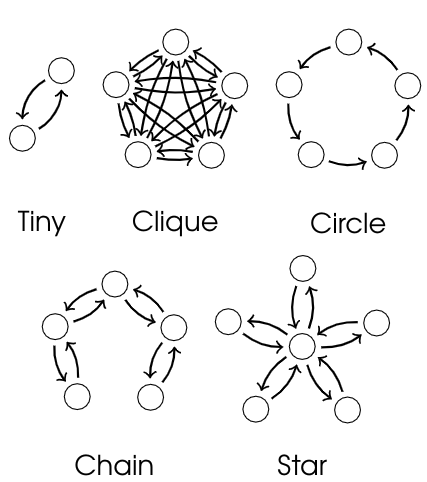
\includegraphics[width=.4\textwidth]{c4/Fig9b.png}
    \caption{Symmetric cycle shapes detected by \textsc{Arcan} and defined by Al Mutawa et al. \cite{AlMutawa2014}.}\label{c2:fig:cycle-shapes}
\end{figure}

\paragraph{God component (GC)}\label{c2:sec:arch-smells-gc}
This smell represents a component (or package, in Java) that is considerably larger in size (i.e. lines of code) than other components in the system \cite{Lippert2006} (see Figure \ref{c2:fig:gc}).
Originally, GC was defined using a fixed threshold on the lines of code, \textsc{Arcan} however uses a variable threshold-detection approach based on the frequencies of the number of lines of code of the other packages in the system \cite{Arcelli2015}.

God components aggregate too many concerns together in a single artefact and they are generally a sign that there is a missing opportunity for splitting up the component into multiple sub-components.
God components tend to become such over time, as a result of several little incremental changes that contribute to the massive scale of the component, which ends up effectively implementing a lot of the overall functionality of the system.
Over time, the understandability of the component deteriorates along with the reusability of the individual parts of the component, because nobody wants to use a piece of software that is difficult to understand \cite{Lippert2006}.

This smell is not part of this study, but it was hereby introduced to keep all the definitions of smells used by the studies in this dissertation in one place.

\begin{figure}[t]
    \centering
    \begin{subfigure}[t]{0.45\linewidth}
        \centering
        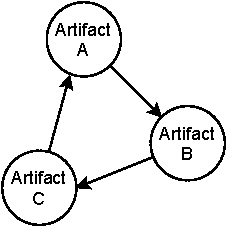
\includegraphics[width=0.5\linewidth]{c4/Fig1a}
        \caption{An example of Cyclic Dependency among artefacts A, B, C.}\label{c2:fig:cd}
    \end{subfigure}
    \hfill
    \begin{subfigure}[t]{0.45\linewidth}
        \centering
        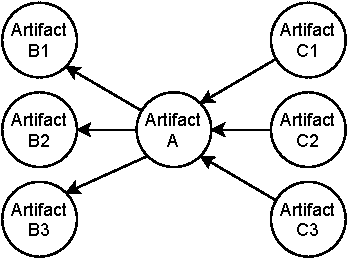
\includegraphics[width=0.7\linewidth]{c4/Fig1b}
        \caption{An example of HL affecting component A, with the afferent (incoming) dependencies on the right and (outgoing) efferent dependencies on the left.}\label{c2:fig:hl}
    \end{subfigure}
    \\
    \begin{subfigure}[t]{0.45\linewidth}
        \centering
        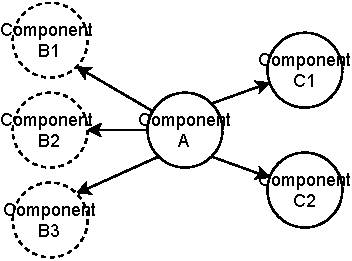
\includegraphics[width=0.7\linewidth]{c4/Fig1c}
        \caption{An example of UD affecting component A. The components that A depends on (Bs and Cs) are shown in the figure too. Components B1 to B3 are less stable than A and represent the majority of A's outgoing dependencies.}\label{c2:fig:ud}
    \end{subfigure}
    \hfill
    \begin{subfigure}[t]{0.45\linewidth}
        \centering
        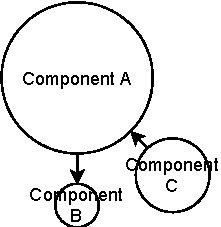
\includegraphics[width=0.5\linewidth]{c4/Fig1d}
        \caption{An example of GC affecting component A. The diameter of A represents its larger size in terms of lines of code w.r.t. other components in the system (B and C).}\label{c2:fig:gc}
    \end{subfigure}
    \caption{Illustration of the four architectural smell types considered in this work.}
    \label{c4:fig:architectural-smells} 
\end{figure}

\subsection{The \textsc{Arcan} tool}\label{c2:sec:arcan}
\textsc{Arcan} parses Java, C, and C++ source code files to create a dependency graph where files, components, classes and packages are all represented using different nodes with different labels. Dependencies, and other relationships between nodes, are represented using edges that connect the dependant to its dependencies with an outgoing, labelled edge (e.g. if artefact \texttt{A} depends on artefact \texttt{B}, then the dependency graph contains a directed edge connecting \texttt{A} to \texttt{B}.). 
The project's structural information contained in the dependency graph is then used to calculate several software metrics (e.g. fan-in, fan-out, instability \cite{Martin2018}, etc.) and then detect architectural smells by recognising their structure in the dependency graph.

Compared to other tools, \textsc{Arcan} uses only software metrics and structural dependencies in order to detect architectural smells. 
This makes \textsc{Arcan} different from tools such as DV8 \cite{Mo2015} (a tool used by related work) which also requires the use of change metrics.
While this type of metrics definitely provide important insights into the maintenance hotspots of the system, they also come with the requirement of needing historical data in order to be used.
This aspect is of particular importance in our case as the version control system adopted by the company we worked with, \emph{did not provide} such information.

Despite the different approaches to detect architectural smells, the two tools,  \textsc{Arcan} and DV8, have some overlap in the detected smells. 
Both tools detect cycles among files and components and both detect hub structures (called \emph{Crossing} by DV8 and Hublike Dependency by \textsc{Arcan}), but DV8 also incorporates historical information for the detection of the latter type of smell.


\subsection{Similarities and differences between code and architectural smells}
Distinguishing between code smells (CS) and AS may not always be easy as different authors have a different understanding of what constitutes one or the other.
In this section, we try to provide a brief explanation about both and clarify the differences between these two concepts.

Code smell is a term first popularised by Kent Beck in the late 1990s \footnote{Read \url{https://wiki.c2.com/?CodeSmell} for more info.} and then further defined by Martin Fowler and Kent Beck himself in the early 2000s \cite{Fowler2002}.
A CS is a sign that the piece of code under inspection requires some changes (i.e. a refactoring) in order to be considered of good quality \cite{Fowler2002}. 
In other words, code smells are symptoms of poor design and implementation choices \cite{Tufano2015}.

The term architectural amell was first adopted by Lippert \cite{Lippert2006} in 2006 to describe a part of the system that required significant refactorings at the architecture level in order to meet the desired quality standards.
To be more specific, Lippert mentions that architectural smells, contrary to code smells, require \emph{large refactorings} in order to be removed from the part of the system they affect and require longer than a day to be applied \cite{Lippert2006}.

Both AS and CS manifest themselves in different forms that are commonly referred to as different \emph{types}.
Some examples of CS types are \emph{Duplicated Code}, \emph{Long Method}, and \emph{Large Class} \cite{Fowler2002}.

Finally, it is important to mention that previous work provides empirical evidence that the AS  considered in this study and the most well-known code smells are \emph{independent} entities and that there is no correlation between the presence of AS and CS \cite{Arcelli2019}.

\subsection{Architectural smell characteristics}\label{c2:sec:smell-characteristics}
An architectural smell characteristic is a property or attribute of an architectural smell instance. 
An architectural smell instance is a concrete occurrence of a type of architectural smell.
For each architectural smell type, one can measure different characteristics. We refer to the characteristics that can be measured for every type of smell as \emph{smell-generic}, whereas we refer to the characteristics that can only be measured for certain types of smells as \emph{smell-specific} characteristics.
The characteristics considered in this work are reported in Table \ref{tab:smell-characteristics}.

\begin{table}[]
    \footnotesize
    \centering
    \caption{The smell characteristics identified by this study. * indicates this study. $^\dagger$ marks characteristics not studied in this study as they are intended as future work.}
    \label{tab:smell-characteristics}
    \begin{tabular}{p{0.035\linewidth}p{0.15\linewidth}p{0.60\linewidth}p{0.025\linewidth}}
    \toprule
    \textbf{Smell} & \textbf{Character.} & \textbf{Description} & \textbf{Ref.} \\ \midrule
    \multicolumn{4}{c}{\itshape smell-generic}\\\midrule
    \multirow{5}{*}{All} & Age & The number of versions affected by the smell. & * \\
     & Overlap Ratio & The ratio of the total number of components of a given smell that also take part in another smell. & * \\
     & Centrality & The importance of the components affected by the smell within the system. Measured using the PageRank of the components in the dependency graph. & (1) \\
     & Size & The number of elements of the system affected by the smell. & * \\
     & Number of edges & The number of dependency edges among the components affected by the smell. & * \\ \midrule
    \multicolumn{4}{c}{\itshape smell-specific}\\\midrule
    \multirow{4}{0.1\linewidth}{CD} & Shape & The cycle shapes as shown in Figure \ref{c2:fig:cycle-shapes}. & (2), (3)\\
    & Average edge weight &  The number of dependencies (weight) between the components affected by the smell. It can be indicative of the difficulty of refactoring the cycle. & (4)\\
     & Number of inheritance edges & The number of edges in the smell that represent an inheritance between components. & (5) \\
     & Affected design level & Whether the cycle is present only at architectural level (among packages) or also at design level (among classes) too. & (3) \\
     & Parent centrality$^\dagger$ & The degree to which a package is at the centre of a cycle with its children sub-packages. & (3)\\ \midrule
     \multirow{2}{0.1\linewidth}{UD} & Instability gap & The difference between the instability of the main component and the average instability of the dependencies less stable than the component itself. & (4) \\
     & Strength (or DoUD (4)) & The ratio between the number of dependencies that point to less stable components and the total number of dependencies of the class. & (4) \\ \midrule
     \multirow{3}{0.1\linewidth}{HL} & Average internal path length$^\dagger$ & Only computed on package HL. The average length of the paths between internal nodes with afferent dependencies and internal nodes with efferent dependencies within the central package. The shorter the length, the more the packages that depend upon the main component and packages that are depended upon by it are connected. & * \\
     & Affected classes ratio$^\dagger$ & Only computed on package HL. The ratio between the number of classes taking part in a dependency relationship with afferent and efferent packages of the main component and the total number of classes in the main component. & *, (6) \\\bottomrule
    \end{tabular}
    (1)\cite{Roveda2018}; (2)\cite{Arcelli2016}; (3)\cite{AlMutawa2014}; (4)\cite{Arcelli2017}; (5)\cite{Laval2012}; (6)\cite{Abdeen2011}
\end{table}

% Why these characteristics?
We decided to focus our analysis on this set of smell characteristics because they are measurable dimensions for the different facets of smells that further quantify the extent to which the smell affects the system; this can  inform developers on how to prioritize refactoring.
Additionally, some of the selected characteristics were developed, studied or discussed by other authors in previous studies, as reported by the Ref. column in Table \ref{tab:smell-characteristics}.

The smell-generic characteristic \emph{Overlap}, \emph{Centrality}, and \emph{Size} are of interest because they are all metrics that are conceptually related to the complexity caused by any instance of a smell in the system. Intuitively, all of them \emph{may} hinder the degree of understandability, extensibility, or generally of maintainability of the components affected by a smell: the more elements a smell has (size), or the more elements of a smell are also involved in other smells (overalp), or the more its elements are interacting with other important components of the system (centrality), the harder it is to fully understand or to refactor the smell. 

\emph{Age}, on the other hand, allows us to track the evolution of the other characteristics over time, identify periods where they are more impactful, or discern eventual correlations between them.

The CD smell-specific characteristics \emph{Shape} and \emph{Average edge weight} are of interest because they are directly related to the complexity of the smell.
The more complex the shape, and the more edges there are between the affected components, the harder the smell is to refactor because more effort is required.
The \emph{Affected design level}, similarly, is important because the cycles present at both package and class level have an impact on two different levels at once.
Finally, the \emph{Number of inheritance edges} characteristic is considered because inheritance edges are considered an indicator of an intentional design choice \cite{Laval2012}, thus intentional cycles that contain a high number of inheritance edges between the components may be more interesting for a developer to inspect.

The UD smell-specific characteristic \emph{Instability gap} and \emph{Strength} are of interest because they are used for the detection of the smell and thus can effectively measure its criticality. The higher the instability gap, the higher the chance the component affected by the smell is changed due to ripple effects \cite{Martin2018}. Likewise, the higher the strength, the higher the chance (because there are more possible components that are prone to a change) a change occurs and propagates to the affected component.

The HL smell-specific characteristics \emph{Affected classes ratio} and \emph{Average internal path length} are of interest because they quantify the involvement of the internal classes in the smell by answering the questions `How many classes belonging to the affected package (out of all package classes) contribute to the smell?' and `How much efferent and afferent packages are actually connected?', respectively.
Intuitively, if the average internal path length is low, it is easier for changes to propagate through the components involved in the smell. And if the efferent and afferent packages are poorly connected (i.e. few paths), the chance a change propagates is small.
In other words, these two characteristics measure the proneness of a HL smell to propagate changes incoming from its dependencies to the components depending upon it.

\section{Case study design}\label{c2:sec:case-study}
The design of the case study follows the guidelines proposed by Runeson et al. \cite{Runeson2012} to conduct and report case studies.
Furthermore, the protocol used to conduct the study and keep track of the changes is based on the template proposed by Brereton et al. \cite{Brereton2008}.

\subsection{Goal and research questions}
The objective of this study is to expand the current knowledge of architectural smells evolution.
Using the Goal-Question-Metric \cite{VanSolingen2002} approach, the objective formulation is:
\begin{quote}\textit{
    \textbf{Analyse} the evolution of individual architectural smells instances throughout the system's history \textbf{for the purpose} of understanding them \textbf{with respect to} their  characteristics and lifespan \textbf{from the point of view of} software architects \textbf{in the context of} open source systems.} 
\end{quote} 
Each one of the research questions that further refine the goal of this study focuses on a different aspect of their evolution: RQ1 studies the evolution trend of each type of smell w.r.t their characteristics, whereas RQ2 studies the survivability (or persistence) of each smell type. 
The two research questions (RQ1 and RQ2) are answered by answering a number of sub-questions (e.g. RQ1a and b for the case of RQ1).

\begin{enumerate}
    \item[\textbf{\textit{RQ1}}] How does each type of architectural smell evolve throughout the system's history?
    \begin{enumerate}
        \item How do the smell characteristics of each smell type (i.e. size, centrality, etc.) evolve over time? 
        \item Is there a correlation between smell characteristics of the same smell type?
    \end{enumerate}
\end{enumerate}
This research question focuses on investigating the evolution of each type of architectural smell through their characteristics and identifying relations among them.
It can provide information for understanding the effects of each type of smell on the system, which can then be used to define refactoring prioritisation rules based on single instances of that type.
Identifying relations is important to avoid using the same information multiple times.
This means that it is necessary to identify eventual correlations among them so that we can determine if we can omit some of the characteristics without losing essential information.

One example of the use of trend as indicator for extra maintenance effort could be the trend of \emph{centrality}, a smell-generic characteristic that measures the degree of connectivity of the elements affected by a smell with the other system's components: the higher the values the more other components are in some way connected to it and thus the more probable for a change to have ripple effects.

\begin{enumerate}
    \item[\textbf{\textit{RQ2}}] How do the different types of smells compare against each other regarding their lifespan?
    \begin{enumerate}
        \item Which types of smells, CD, HL or UD, are more persistent (i.e. are less common to be removed)?
        \item Do the same smell types at package and class level have a different survival probability?
        \item Does the shape of a CD smell affect its lifetime?
        %\item Which types of smells are more likely to generate other smells?
    \end{enumerate}
\end{enumerate}
The aim of this research question is to compare the different types of smells in terms of their survivability. Answering this question could help to define prioritisation rules at the level of smell type.
For example, one could choose to first refactor the types of smells that are more likely to persist longer within the system.

We decided to focus on survivability because it is a time-based measurable dimension of architectural smells, affecting future maintenance: the longer an AS affects a system, the longer the developers and architects will spend extra maintenance effort on the affected components.

\subsection{Case selection}
In this study, we used a set of open source systems known as the Qualitas Corpus (QC) \cite{QualitasCorpus2010}.
We decided to work with open source systems (OSS) for the following reasons: OSS are easy to retrieve and manipulate, the QC has a big variety of different projects ready to be used, and it is easier to develop static analysis tools when there is the possibility to inspect the source code analysed. An extension ot our analysis on industrial systems is described in Chapter \ref{chap:4}.

The QC has more than 100 projects that can be potentially analysed. We required that projects have more than 15 versions available so to ensure smells have enough time to grow, evolve, and fade, thus limiting  the number of candidate projects to 15.
We also removed EclipseSDK from our selection due to its size causing difficulties during tracking.
The demographics of the selected projects are shown in Table \ref{tab:projects}.

\begin{table}[]
    \centering
    \caption{The projects from the Qualitas Corpus release 20130901e used in this study. A total of 524 versions (both major and minor) were analysed.}
    \label{tab:projects}
    \begin{tabular}{@{}lllll@{}}
    \toprule
    \textbf{Project} & \textbf{\# Versions} & \textbf{First version} & \textbf{Last version} & \textbf{\# Unique AS} \\ \midrule
    Ant & 23 & 1.1 & 1.8.4 & 1211\\
    Antlr & 22 & 2.4.0 & 4 & 1183 \\
    ArgoUML & 16 & 0.16.1 & 0.34 & 3886 \\
    Azureus & 63 & 2.0.8.2 & 4.8.1.2 & 108796 \\
    Freecol & 32 & 0.3.0 & 0.10.3 & 13259 \\
    Freemind & 16 & 0.0.2 & 0.9.0 & 994 \\
    Hibernate & 115 & 0.8.1 & 4.2.2 & 13551\\
    JGraph & 38 & 5.4.4 & 5.11.0.1 & 249\\
    JMeter & 24 & 1.8.1 & 2.9 & 1846\\
    JStock & 30 & 1.0.6 & 1.0.7c & 927 \\
    Jung & 23 & 1.0.0 & 2.0.1 & 238 \\
    JUnit & 24 & 2 & 4.11 & 164 \\
    Lucene & 35 & 1.3.0 & 4.3.0 & 1126 \\
    Weka & 63 & 3.0.1 & 3.7.9 & 2164 \\ \bottomrule
    \end{tabular}
\end{table}

\subsection{Tooling}
To perform the study, we developed a toolchain that allows to mine architectural smells from a series of precompiled Java systems, as illustrated in Figure \ref{c2:fig:data-collection}.
The toolchain is composed of two parts: AS \emph{detection} and AS \emph{tracking}.
\begin{figure}
    \centering
    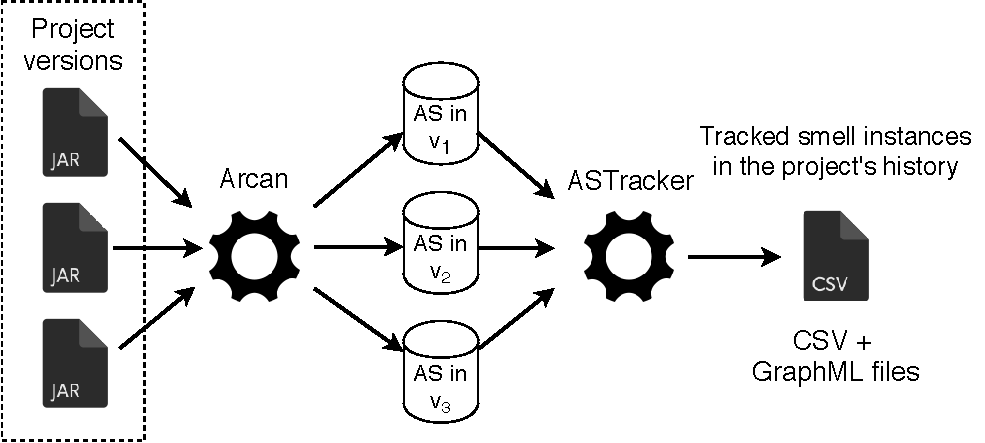
\includegraphics[width=0.8\textwidth]{c2/data-collection-process-pager.pdf}
    \caption{Data collection process and tooling. The data of each individual project was then merged in a single data set.}\label{c2:fig:data-collection}
\end{figure}
\subsubsection{Architectural smell detection}
To identify architectural smells we use \textsc{Arcan}\footnote{\label{fn:Arcan}See \url{https://gitlab.com/essere.lab.public/Arcan}.}, a free Java tool for detecting architectural smells in a system.
\textsc{Arcan} receives as input one, or multiple, JAR files of a single version of a system and outputs a series of CSV files and a GraphML file. The graph file is the dependency graph of the given system extended with nodes denoting architectural smells. The same information as the graph file is contained within multiple CSV files.

\subsubsection{Architectural smell tracking}
In order to perform the study, we needed to track the architectural smells for each pair of consecutive versions of the system, i.e. from $v_1$ to $v_2$, from $v_2$ to $v_3$, and so on.
To this end, we developed a tool, ASTracker\footnote{\label{fn:astracker}See \url{https://github.com/darius-sas/astracker} to access the tool and the data used in this study.}, that performs the following steps: it takes as input multiple versions of a system (the GraphML files produced by \textsc{Arcan}) and maps every smell in each version to its closest successor in the next version, calculates the smell characteristics, and returns the results as CSV and GraphML files.

To perform the mapping of each smell to its successor we use a function $J$ known as \emph{Jaccard similarity index} \cite{Jaccard1912}, defined as
$$J(A, B) = \frac{|A \cap B|}{|A \cup B|}$$
where $A$ and $B$ are the sets of the affected components in two consecutive versions.
The index simply measures the percentage of elements that are shared by the two sets.
The use of this methodology and of the Jaccard index are justified because a smell is defined by the elements it affects: the similarity of the affected sets of elements leads to identifying the successor of a smell.

The comparison among elements in the sets is made using the full name of the classes/packages.
The main advantage of this method is that it avoids name conflicts; however, a renaming in any of the parent packages results in the inability to track the smell in the next version.
Thus, for every smell $k$ in version $v_1$ and for every smell $l$ in version $v_2$, we compute $j_{kl} = J(a(k), a(l))$ which is basically a matrix where the rows are the smells from $v_1$ and the columns are the smells from $v_2$. 
The function $a$ returns the set of elements affected by a smell.
The linking between smells $k$ and $l$ is done using a \textbf{greedy strategy}:
the highest $j_{kl}$ such that $k$ and $l$ have not already been linked with another smell, is the next mapping $k \rightarrow l$ to be created.
The greedy strategy ensures that every smell has been linked with the smell that is most similar to itself, which means formally that only one cell per row and column from the matrix $j$ is selected.
This operation is repeated until there are no more smells left to map or the similarity scores of the remaining ones do not satisfy $j_{kl} \geq \theta$, where $\theta$ is the similarity threshold defined as
\begin{equation*}
\theta = \begin{cases}
     0.67   & \text{ for } |a(k)| > 5 \\ 
     0.60   & \text{ for } |a(k)| \leq 5 \\
    \end{cases}
\end{equation*}

We selected a variable threshold in order to cover the big variance of the function $J$ when $a(k)$ has a relatively small cardinality.
To adjust the thresholds, we consulted all the possible values of $J$ in the case where the two inputs shared all of their elements but only the size changed.
Additionally, we also consulted all the possible values for small input sets sharing a variable number of elements.
The selection of $\theta = 0.60 $ when $|a(k)| \leq 5$ allows for a maximum difference of 3 elements with a smell's successor, allowing the algorithm to be more permissive for smells with fewer elements.
Likewise, a value of $\theta = 0.67$ allows for a reasonable variation when the size of an AS is bigger than 5.

The algorithm only maps smells of the same type, namely CD with CD, UD with UD, and HL with HL.
% \begin{figure}
%     \centering
%     \includegraphics[width=0.45\textwidth, trim = {0.2cm 0.1cm 0.1cm 0.2cm}, clip]{jaccard-scores-bw.png}
%     \caption{Jaccard similarity scores for each pair of smell size (up until 16 and 10). The linking intervals are shown in red squares. In the figure it is assumed that the elements affected are always the same.}\label{c2:fig:jaccard-scores}
% \end{figure}

\section{General results}\label{c2:sec:general-results}
This section introduces some general statistics and insights concerning the data we have collected\footnote{\label{fn:supp-mat}Supplemental material available at \url{http://www.cs.rug.nl/search/uploads/Resources/supp-material-as-evo-icsme19.zip}.}.

\subsection{Smell density}
A good starting point in understanding the evolution of smells is to look at the smell density (\# of smells per component).
As the smell density in a system gets closer to one it means that, on the average,  there is one smell for every component in the system.
Figure \ref{c2:fig:smell-count} shows the density of each smell type across the versions of every system. 

Remarkably, seven projects have a smell density for CD among packages that is either higher or very close to 1 in most of their versions, meaning that it is quite common for developers to create cycles among the packages of the systems, thus increasing the complexity of the system.
It is interesting though to note that the density of CD among classes, in most of the systems, is more or less constant throughout time despite the size of the systems growing (i.e. their ratio remains mostly constant).
In other words, CD smells at class level are constantly introduced by developers as a by-product of the development activities as the system evolves.
This causes also the number of cycles among packages to increase (because some of those cycles will be among classes from different packages), and since the number of classes per package increases over time in most of the systems analysed the smell density on packages is bound to increase as well.
A similar pattern also emerges for UD smells, which are also constantly introduced in the system and have a growing trend.
On the contrary, the number of HL smells stays mostly constant and relatively low (less than 10) over time in all the systems analysed, which is expected as a system has only few components that have a disproportionate number of dependencies.

\vspace{1mm}
\fbox{\begin{minipage}{0.95\linewidth}\small
    \textbf{Takeaway}\\
    Dependencies across packages affected by CD smells become ever tighter as the system ages, making it more difficult over time to reuse them seperately, without importing the whole system.
    This is caused because the cycles among packages grow in number at a higher rate than the number of packages itself.
\end{minipage}}

\begin{figure*}
    \centering
    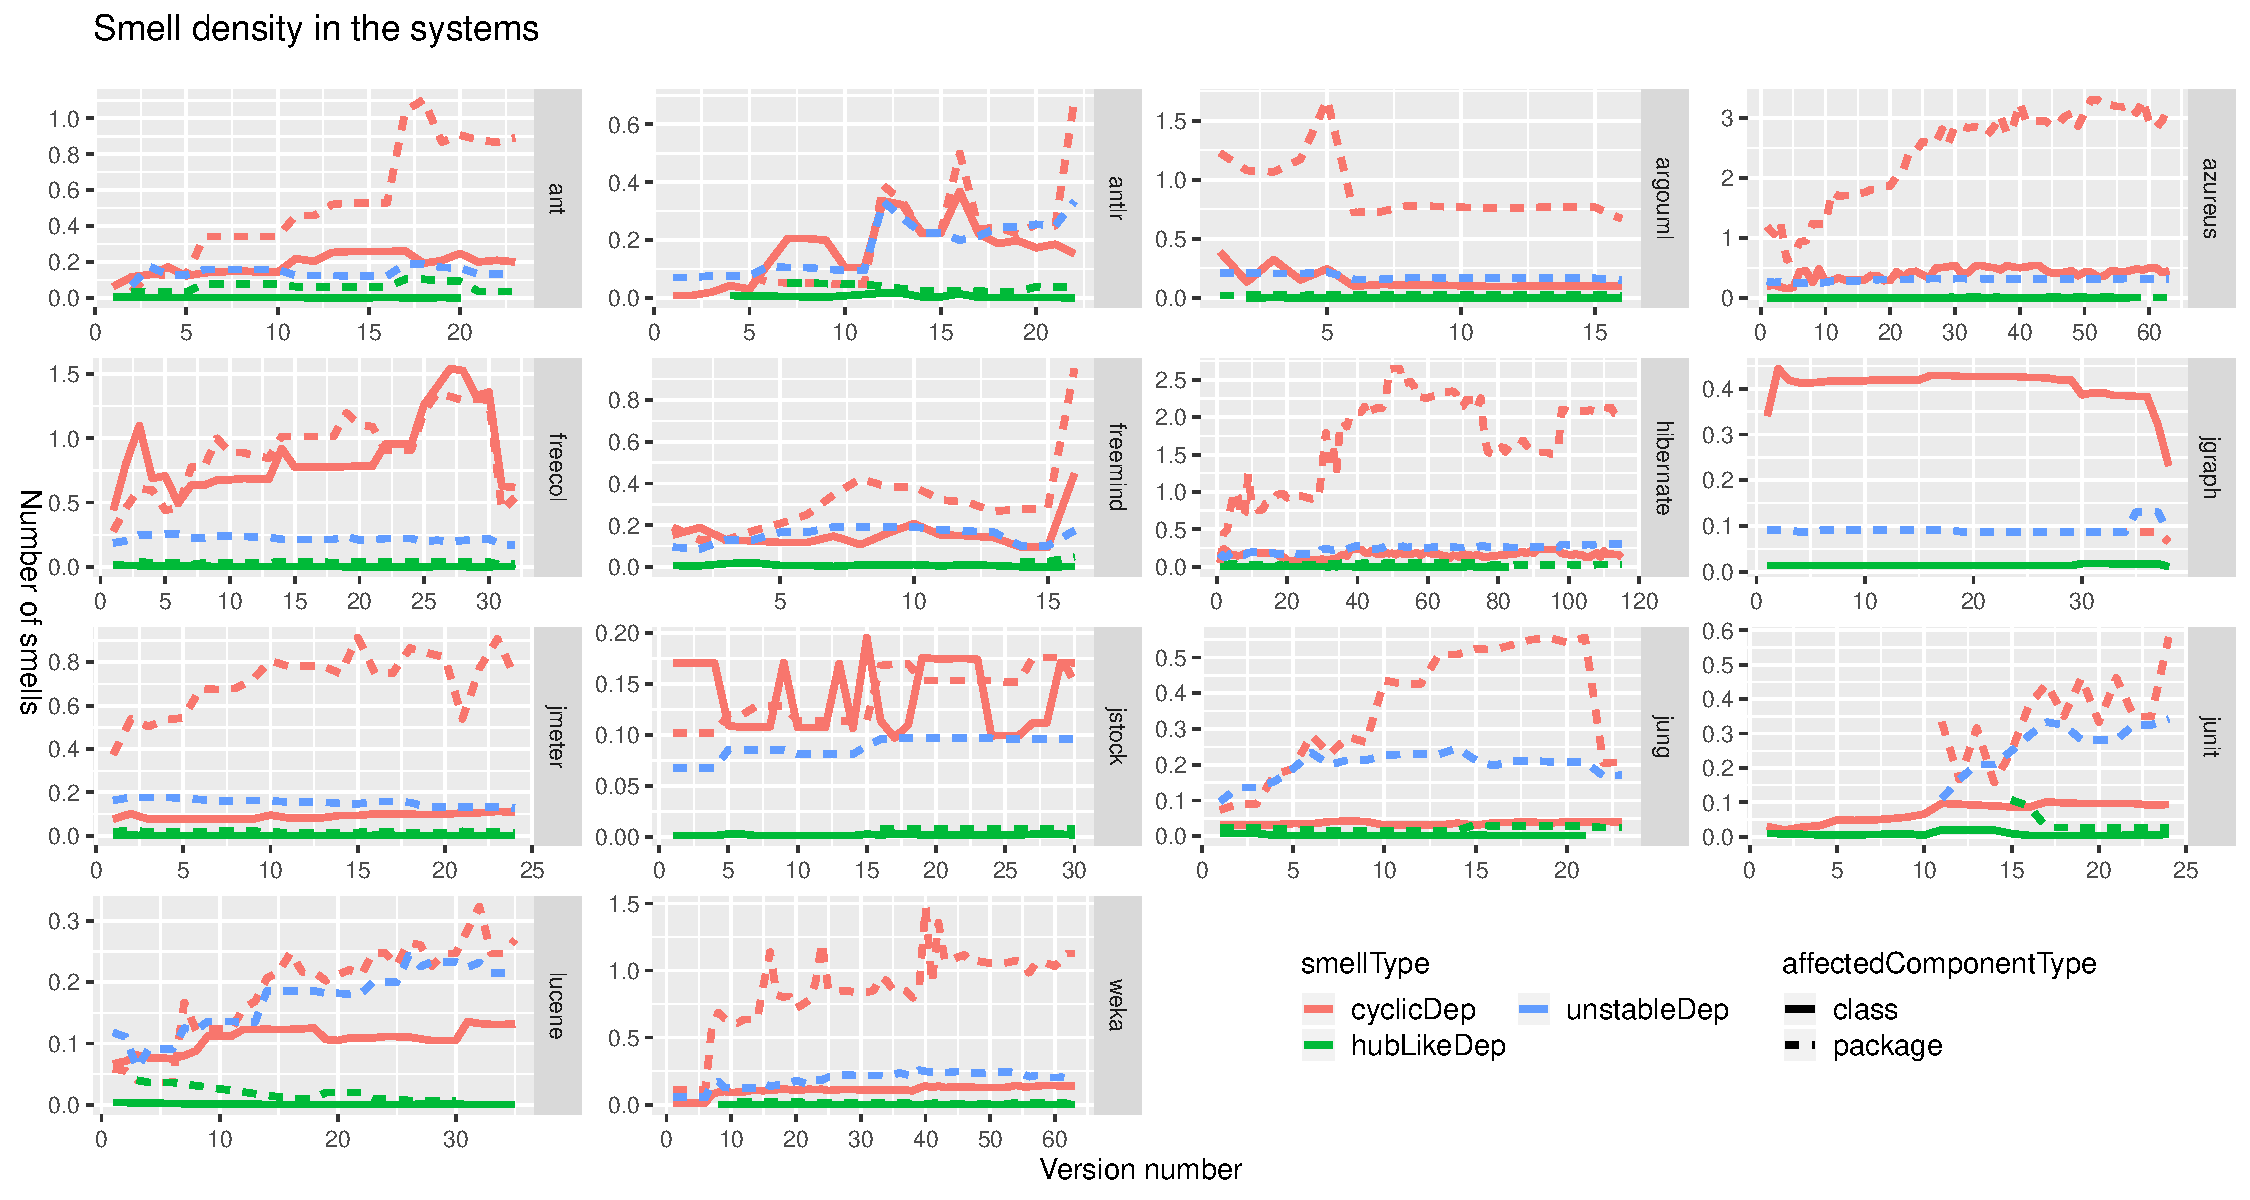
\includegraphics[width=\textwidth]{c2/descriptive-smell-density.pdf}
    \caption{Number of smells in the system divided by total number of classes or packages, depending on the type of the component affected.}\label{c2:fig:smell-count}
\end{figure*}

\subsection{Smell characteristics}\
In this section, we briefly cover some interesting findings on the characteristics mentioned in Table \ref{tab:smell-characteristics}.
One noteworthy finding is the difference in size between smells. HL smells, due to their definition, tend to be usually bigger than the other types of smells, surpassing 100 elements in bigger systems, whereas UD smells are the smallest ones, hardly surpassing 10 elements even in bigger systems.
However, CD and UD smells have higher overlap ratio in general, meaning that trying to refactor a smell with high overlap will entail also dealing with a certain number of other smells.

Concerning UD smells specifically, we note that their instability gap mostly ranges between $-0.1$ and $-0.3$; since these values are relatively close to zero, we argue that they are not very prominent and by slightly improving the instability of few packages, the smell could be removed.
However, the instability gap is also decreasing over time for 50\% of the UD smells detected (more details on this analysis in Section \ref{c2:sec:rq1a-results}), meaning they become more severe over time. 

Finally, we also note that CD smells are mostly at the class level only\footnote{See 'Affected design level' in Table \ref{tab:smell-characteristics} for more details.} (ranging from 60\% to 95\%, depending on the project) or package level only (from 0 \% to 75\%, depending on the project).
A small percentage (less than 3\%) affects class and package level at the same time and an even smaller percentage (1-2\%) switch between levels over time (e.g. they go from class level only to both architectural and class).

\section{Trend analysis (RQ1a)}\label{c2:sec:rq1a-results}
\subsection{Methodology: dynamic time warping}
Analysing the trend of all the characteristics of each smell instance detected in the analysed systems was not a trivial problem to solve, due to its dimensionality (smell instances, time, characteristic).
The approach adopted to solve the aforementioned problem was signal classification: the values assumed by a certain characteristic for a certain smell over time are considered as a signal, then they are compared to a series of predefined signals and a label is assigned to each one of them based on the \emph{distance} from each template.
We used dynamic time warping\footnote{The implementation used for this analysis was provided by the R package \texttt{dtw}.} \cite{Kruskal1983} to warp the signal of each template and stretch it to match the signal one desires to compare it with. 
This technique was previously used by Vaucher et al. to classify the trend of God Classes \cite{Vaucher2009}.

Formally, we can model the problem as follows: for every smell characteristic $C^{k}$ of a certain smell $k$ we consider the different values $C^{k}_i$ as a signal $S$. We then compute the following variables: $h = \max S$; $l = \min S$; and $m = (h+l)/2$.
These three values are then used to build the seven templates, named from $a$ to $g$, as shown in Figure \ref{c2:fig:classification-templates}. For example, temblate (b) is defined as $b = (l, m, h)$.
The templates are re-adjusted for each signal classified.
Finally, the signal is classified by comparing the distance of the signal from each template, and selecting as a label the template name of the closest signal template. 
Specific implementation details can be inspected in the source code.

\begin{figure}[]
    \centering
    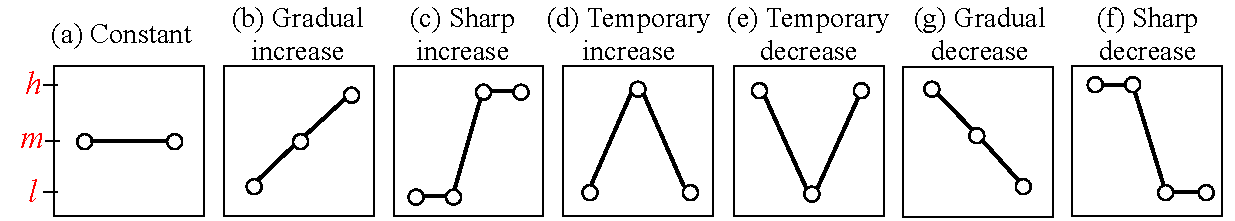
\includegraphics[width=\textwidth,trim={0.2cm 0 0 0},clip]{c2/dynamic-time-warping-min-1line.pdf}
    \caption{Trend evolution classification templates. Figure adapted from the work of Vaucher et al. \cite{Vaucher2009}.}\label{c2:fig:classification-templates}
\end{figure}

Despite the selected templates offering a good variety of possible signal shapes, there may be some cases that are not described well enough by the current selection. For example, signals that vary between two integer values (e.g. 6-7) multiple times, would be classified by the model as a constant signal (i.e. template (a)).
Nonetheless, we deem that the approximation offered by the model when unusual signal curves have to be classified is sufficient for the purpose of this chapter for the following reasons:
\begin{itemize}
    \item the templates selected represent simple and general cases, thus they simplify interpretation and analysis;
    \item a signal is classified based on the distance between points from the template and points from the signal itself after being warped, thus the classified signal has at least an internal component that resembles the classification tag (i.e. template) assigned.
\end{itemize}

\subsection{Results}
We performed the aforementioned analysis for all of the numeric characteristics we have recorded.
Hereby we report only the most interesting ones, as there is a large number of data and results that could not realistically fit into this chapter.
\paragraph{Size}
Overall, the size of the smells stays constant throughout their evolution, especially in the case of CD and UD. This is shown in Figure \ref{c2:fig:signal-all} where approx. 50\% of the total CD and UD across all systems have a constant trend.
Instead of growing in size, CD smells tend to grow in number, spreading across the system as new elements are added to the system's dependency network (i.e. new classes, packages, etc.).
Nevertheless, there is a fair amount of smells among all the types that exhibit an increasing trend of some kind (types B, C, D).
Specifically, HL smells tend to grow in nearly 65\% (40\% Sharp and 25\% Gradual increase) of the cases. Given its nature, having a hub that keeps getting bigger and bigger through dependencies from more and more classes, or packages, is problematic: that part of the system becomes more complex, it has a lower cohesion and a higher coupling, thus hindering future maintenance activities on it.
It is thus important to \emph{limit the growth} of such smells by redistributing the responsibility of the central component affected by the smell to others.

\paragraph{Number of Edges}
Contrary to size, the number of edges connecting the components affected by a smell have a different trend: they tend to increase.
Specifically, as can be seen in Figure \ref{c2:fig:signal-all}, each smell type exhibits an increasing trend in the number of edges involved in the smell of at least 40\% and up to 80\%.
Additionally, the number of edges between the affected components grows faster than the number of components per se.
Again, this is especially true in the case of HL smells, making them the type of smell that grows faster among the smells studied in this work.
Hublike dependencies are thus an important source of extra maintenance effort, and the number of edges among the affected components of an HL smell can quantify this effort more precisely than the number of affected elements. 
Indeed, this makes sense because an increasing number of edges between components also increases the probability that a change propagates to adjacent components that depend on the component subject to change (as described in Section \ref{c2:sec:arch-smells-hl}).
This fact was also mentioned in a previous work on change proneness metrics of software packages, where the number of method calls (and thus also dependencies) has been used as a change proneness indicator \cite{Arvanitou2015}. Additionally, Martin also links dependencies with change proneness \cite{Martin2018}.

\paragraph{Centrality} 
The centrality metric selected is PageRank \cite{Roveda2018}. We decided to measure the PageRank of a smell as the maximum PageRank value of the affected components and then weight it against the number of elements in each version.
This weighting makes sense because as the system ages, also the number of nodes in the graph used for the calculation of the PageRank increases, scaling down its values, but maintaining the proportions, hence the weighted version allows us to account for this phenomenon.

As one can observe in Figure \ref{c2:fig:signal-all}, as the system and the smells age, the centrality of the smells tends to increase in the vast majority of the cases, especially for CD and HL. On the other hand, UD exhibit more or less the opposite trends.

The results indicate that the component with the highest PageRank (which is very likely to be the central component) in HL smell tends to \emph{``move''} to the centre of the system as the system ages. A similar trend can be observed for CD smells too.
These results confirm a very important assumption for these two types of smells: \emph{AS tend to move to more central parts of the system as they age}. These central parts are also the most important as they have many ingoing dependencies. Consequently, increasingly more maintenance is required for the parts of a system that are affected by CD and HL smells. 

Unexpectedly, for UD one can observe the opposite since most of them exhibit a decreasing trend (types E, F, and G).

\vspace{1mm}
\fbox{\begin{minipage}{0.95\linewidth}\small
    \textbf{Takeaway}\\
    Hublike dependency smells are a better target for refactoring activities in terms of reduction in complexity, future maintenance efforts, and ease of removal for refactoring activities are likely to focus mostly on the central component, by moving functionality elsewhere, rather than on several components as in the case of multiple CD smells.
\end{minipage}}

\begin{figure}[t]
    \centering
    \begin{subfigure}[]{.8\textwidth}
        \centering
        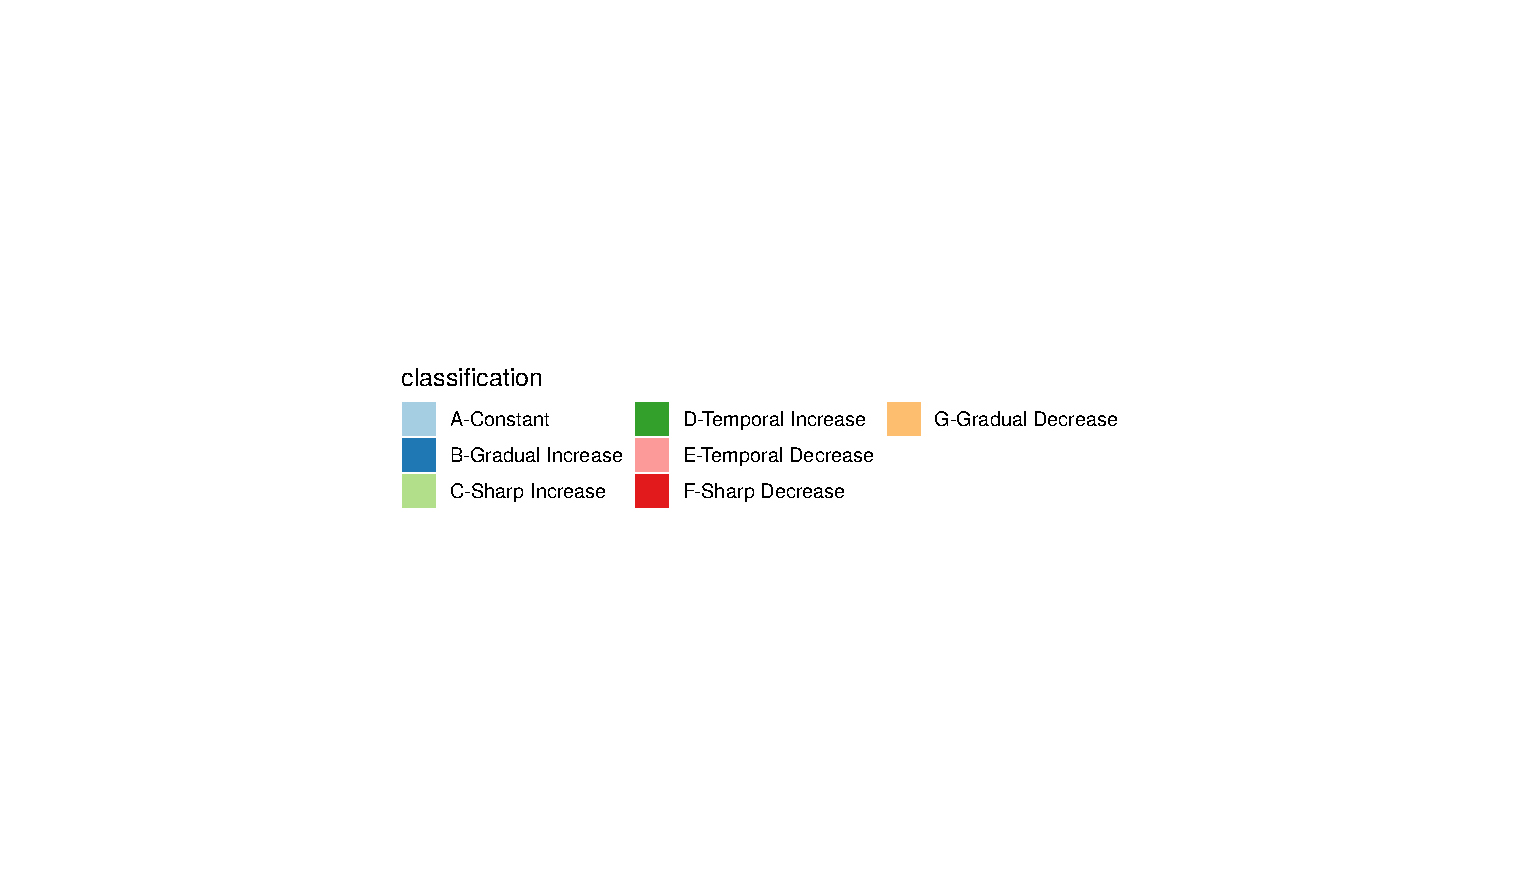
\includegraphics[width=\linewidth,trim={6cm 6cm 6cm 6cm}, clip]{c2/signal-trend-legend.pdf}
    \end{subfigure}
	\hfill \\
    \begin{subfigure}[]{.8\textwidth}
        \centering
        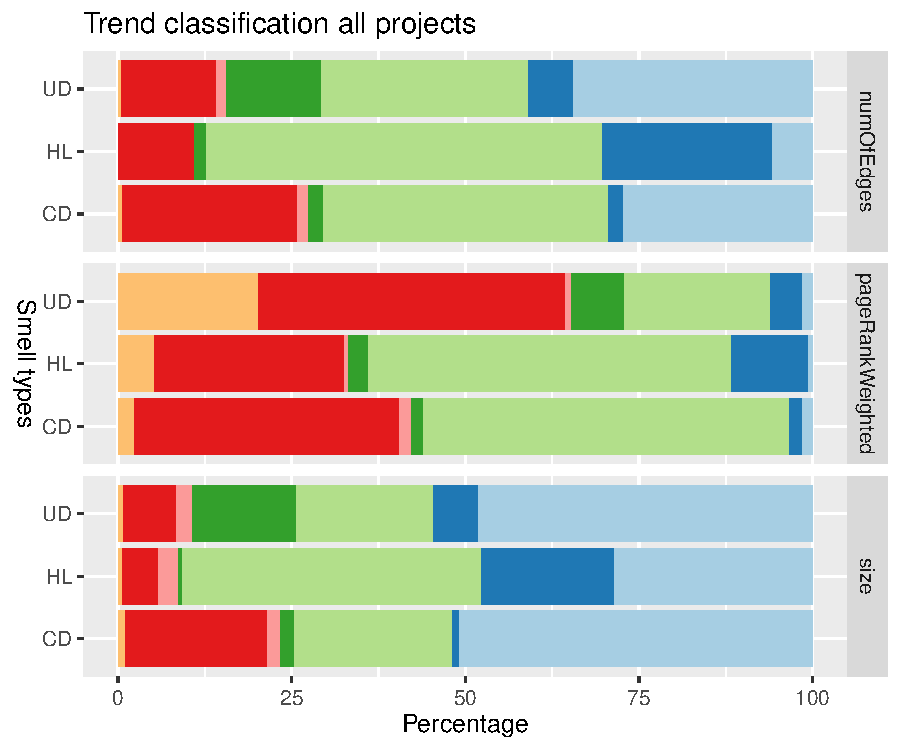
\includegraphics[width=\linewidth]{c2/signal-trend-all-projects-oneplot.pdf}
    \end{subfigure}
    \caption{Signal classification distribution for different characteristics aggregated for all projects as percentages of the total number of smells of that type.} 
    \label{c2:fig:signal-all}
\end{figure}

\section{Correlation analysis (RQ1b)}\label{c2:sec:rq1b-results}
To identify related \textit{pairs of characteristics} for each smell instance of the same type, and for each pair of characteristics, we ran a Spearman correlation test to check for eventual correlations. 
The test was selected because the data is not normally distributed and it is not possible to assume that there is any linear relationship among all the characteristics neither.
The test was performed on each smell instance and only on the pairs of smell characteristics whose both standard deviations were not equal to zero for that instance.
The aggregate test results for all smells were plotted using boxplots (only $p \leq .05$).
The plots are included in the online supplemental material for space reasons.

The characteristics that present a correlation for the majority of the instances detected are the following:
\begin{description}
    \item[Num. of edges $\sim$ Overlap\footnote{The notation $C^1 \sim C^2$ reads `$C^1$ correlates with $C^2$'.}] for smells of type HL and CD at package level. This is expected because of the high smell density at package level (as shown in RQ1a).
    UD, however, do not present such a correlation for these characteristics; this is probably because they usually do not affect central parts of the system, which are more likely to be affected by multiple smells.

    \item[Num. of edges $\sim$ Centrality] for HL smells at class level.
    This was also expected due to the definition of HL (i.e. a component with a lot of incoming and outgoing dependencies, which increases PageRank by definition).
    CD at class level also exhibit a correlation for these two characteristics, but a bit weaker, probably because CD are more frequent among elements near the center.
    %, which is of course expected.

    \item[Num. of Edges $\sim$ Size] strongly for all smells, which is expected.
    
    \item[Overlap $\sim$ Centrality] only weakly. The most prominent correlation is for HL at class level, but is once again expected.
    
    \item[Overlap $\sim$ Size] for CD at class and package level, is also expected, as the bigger the size, the more likely it is that the elements affected are also affected by other smells. The correlations also exist for HL smells, though they are a bit weaker.
          
\end{description}

Number of edges seems to be correlated with a number of characteristics in multiple cases. Despite this result, it is hard to state that, based on this correlation, one should ignore the other characteristics, as these correlations mostly refer to the \textit{majority of the instances} rather than being an absolute gauge of the general case.
In fact, the only pair of characteristics that one can state that are fully correlated for all smell types, independently of the instance, are Size and Number of Edges.
The other correlations are either not valid for all of the smell types, or only a part of the instances analysed show solid evidence of correlation. 

\section{Survival analysis (RQ2a,b,c)}\label{c2:sec:rq2-results}
\subsection{Methodology: the Kaplan-Meier estimator}
The rate of survivability of an architectural smell within a system may drastically vary depending on its type. To establish the rates and compare them among the different projects and smell types, we employed a technique typically used in the biomedical sciences, in product reliability assessment, and also employed to analyse code smell persistence in previous studies \cite{Chatzigeorgiou2014}.
Unlike simple descriptive statistics, such as mean, density functions, and similar, survival analysis also takes into consideration the possibility that a smell continues to affect the system even after the last version included in the analysis.
In the biomedical domain, this event is associated with the patient surviving past the period of the analysis.
%More technically, this type of data is said to be \emph{right-censored}, because the outcome of the treatment could not be measured, generally, due to the conclusion of the study.

The survival analysis is accomplished using the Kaplan-Meier estimator \cite{Kaplan1958}, a non-parametric statistic that estimates the survival probability of a type of smell as the system evolves (new versions are released).
The statistic gives the probability that an individual patient (i.e. smell in our case), will survive past a particular time $t$.
At $t = 0$, the Kaplan-Meier estimator is equal to 1, and as $t$ goes to infinity, the estimator goes to 0. Also, the probability of surviving past a certain point $t$ is equal to the product of the observed survival rates until $t$.

\subsection{Results}
Figure \ref{c2:fig:survival} reports the results of the analysis, i.e. the survival probabilities (a) of different smell types and (b) of different cycle shapes.

\begin{figure}[h]
	\centering
    \begin{subfigure}[]{.7\textwidth}
        \centering
        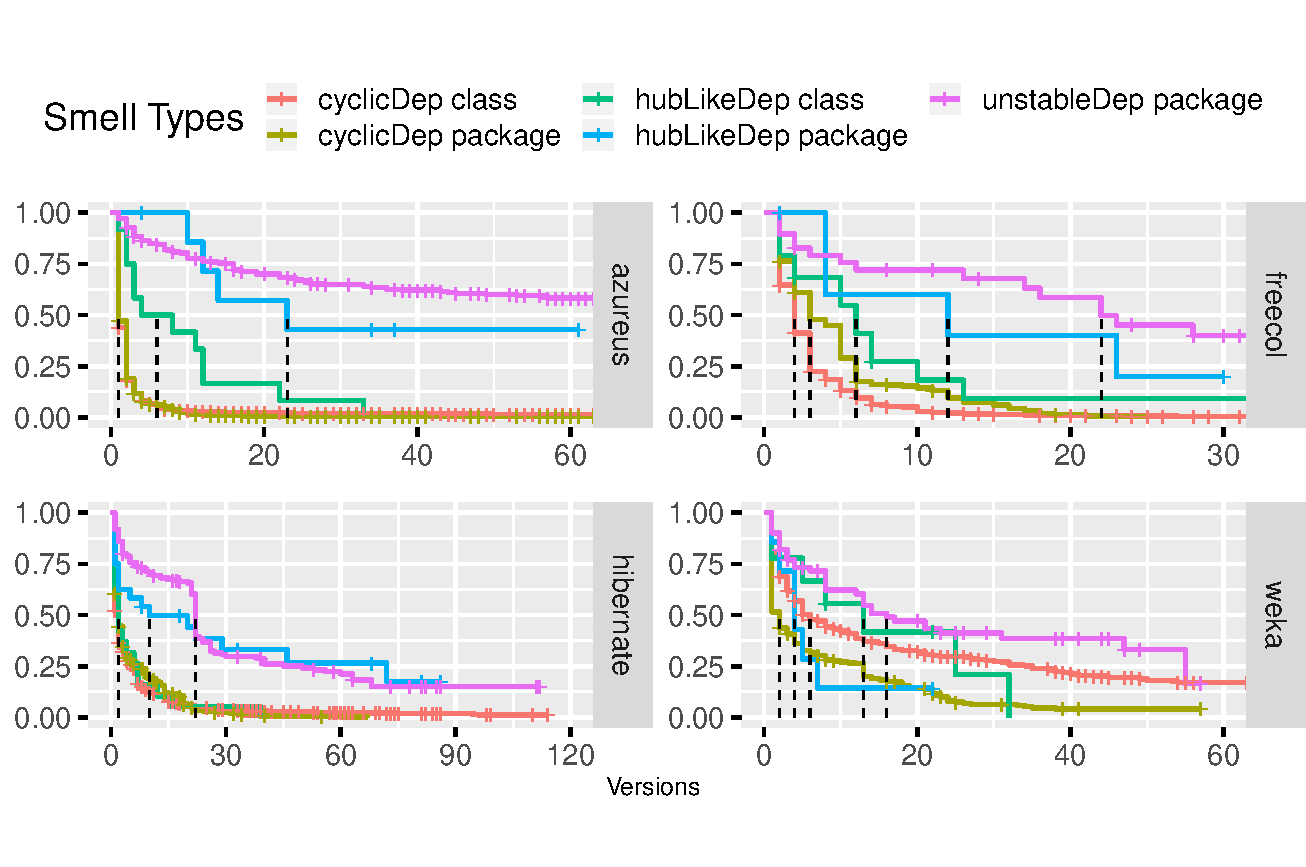
\includegraphics[width=\linewidth, trim={0 0.8cm 0 1cm}, clip]{c2/survival-probabilities-selection.pdf}
        \caption{Smells of different types affecting classes or packages.}
        \label{c2:fig:surival-smells} 
    \end{subfigure} \hfill \\
    \begin{subfigure}[]{.7\textwidth}
        \centering
        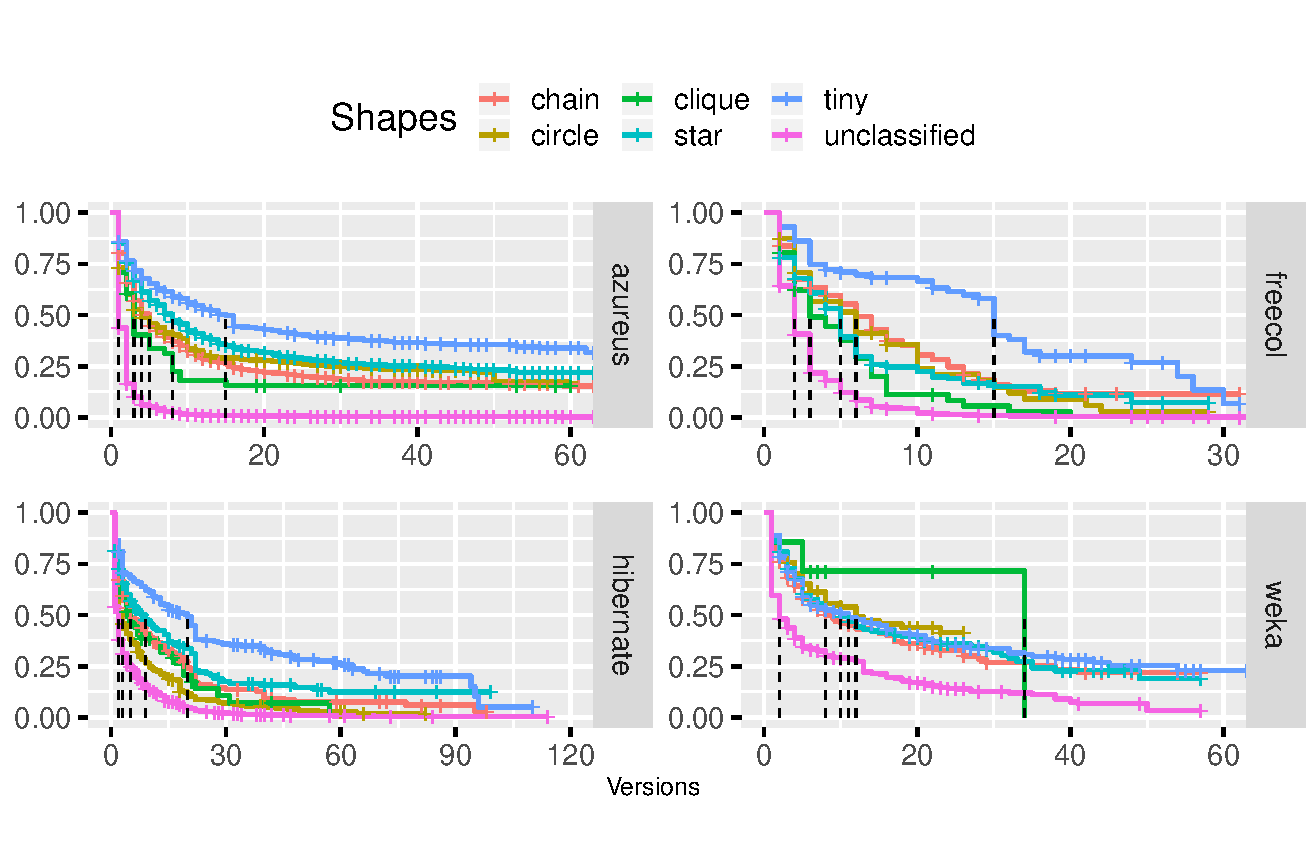
\includegraphics[width=\linewidth, trim={0 0.8cm 0 1cm}, clip]{c2/survival-probabilities-shapes-selection.pdf}
        \caption{Cyclic dependencies of different shapes.}
        \label{c2:fig:survival-shapes} 
    \end{subfigure}
    \caption{Survival probability $p$ up until any time $t$. $p = 0.50$ is represented by a vertical dashed line. Only a selection of systems is shown here for the sake of readability. The full plot is available in the online supplemental material.}
    \label{c2:fig:survival}
\end{figure}

\subsubsection{Survival probabilities of different smell types (RQ2a,b)}
One pattern that emerges from Figure \ref{c2:fig:survival}a is that CD smells fade much quicker than the other types of smells in almost all of the systems and have a very small probability to persist within the system for a long time.
We conjecture that the cycles that persist the most are the cycles among the fundamental components of the system; these are very unlikely to change after the core development activities for that part settle down and new functionalities attract the effort of developers.
Moreover, we also note that cycles only have a \emph{50\% chance} to stay within the system for more than 4-5 releases. Furthermore, cycles among classes persist a little longer within the system than cycles among packages, probably because classes taking part in cycles at design level only might have a stronger coupling with each other than packages.

Another pattern that emerges is that UD is the most persistent type of smell, being the one with the highest survival probability in the long run.
Its survival probability is so high that in some systems it never falls below 50\%, even when there are a lot of versions such as in the case of Azureus.
Moreover, it also decreases at a much slower rate than the other types of smells, making it an ideal target for refactoring to avoid extra maintenance effort in the long run.

HL smells, are more or less in between the other two smell types. They exhibit a similar decrease rate in survival probability as CD smells but eventually end up surviving for more releases. However, this pattern does not hold for all the projects, and in some cases, HL smells end up being removed within fewer versions than CD.
This trend holds true especially for HL at the class level, which tend to decay much faster than HL at the package level.
Thus, it is reasonable to state that HL at package level can be prioritised over HL at class level as they have a higher chance of requiring extra maintenance over time.
In general, from this analysis one can conclude that package level smells, such as UD and HL on packages, tend to last a little bit longer than class level smells, implying that smells at the package level are potentially more impactful on maintenance efforts than smells affecting classes only.

\fbox{\begin{minipage}{0.95\linewidth}\small
    \textbf{Takeaway}\\
    The refactoring prioritisation should \textbf{not focus on cyclic dependencies} that were recently introduced, as it is very likely that they will disappear within the next few releases because they are less likely to influence the maintenance effort on the long term.
    Instead, refactoring should first focus on either UD smells or HL smells among packages as they exhibit higher persistence rates.
    This also confirms that most circular dependencies are not critical \cite{AlMutawa2014}.
\end{minipage}}\\
\subsubsection{Survival probability of different CD shapes (RQ2c)}
Concerning the different shapes of CD smells, Figure \ref{c2:fig:survival-shapes} shows how different shapes persist within the system.
The results show that the most pervasive shape in most systems are tiny shapes. This makes sense as tiny shapes are composed by only two elements and there might be multiple dependency edges between the two elements; thus the probability of a tiny cycle to break is smaller than shapes with multiple elements.
Additionally, tiny cycles are easier to understand and may also be intentionally designed as such.

On the other hand, the other, more complex, shapes are less \emph{resilient} (i.e. they disappear faster than tincy cycles) and there is very little difference between different shape types, making it hard to formulate any solid proposition on their survivability. In order for these complex shapes to persist, they must affect parts of the system that have a solid conceptual connection; otherwise they do not persist long within the system.

Regarding instead the cycles \textsc{Arcan} could not classify into definite shapes, they have a more consistent trend and disappear quicker than all other shapes.
A possible explanation could be related to their nature: we conjecture that this type of cycle is mostly random and caused by casual relationships among components that tend to connect multiple uncomplete cycles into a single one, possibly overlapping with other cycles as well.
Thus these very volatile edges that interconnect multiple parts of a system have a high chance of getting changed because they are individual edges, and if one of these edges is removed, the whole cycle breaks.
This is also evident from the clear difference in survival probability between the unclassified shapes and the complex shapes (circle, chain, clique, star).

\fbox{\begin{minipage}{0.95\linewidth}\small
    \textbf{Takeaway}\\
    We suggest that tiny shapes should not to be prioritised during refactoring even though it is the most persistent one, as it may be the \textbf{result of intentional design} (false positives).
    Refactoring activities, instead, should prioritise old cycles with complex shapes that  are more likely to affect important parts of the system, and thus that are more likely to incur extra maintenance effort.
\end{minipage}}
%IMPORTANT ADDITION FOR CAMERA READY
%We hypothesise that this is imputable to the highly connected network that a system grows into as more and more components (due to new functionality, probably) are added. Hence, as soon as a single edge, or node, changes within this intricate network, one or multiple cy-cles are broken or created, which is also confirmed by the high overlapping between smells and the ‘less-constant’ trend of the characteristic number of edges. This has an important consequence on the smells that one should consider refactoring, both type-wise and in-stance-wise.

%\section{Discussion}\label{c2:sec:discussion}

% Smell density constant to project size
% Smells tend to move to more central parts of the system
% CD stable in size, but grow rapidly in number
% CD smells decay much quicker than other smell types
% Tiny shapes are most persistent probably due to the ease of creating them as intentional design
% Unclassified shapes, and CD in general, may be the result of casual relations among components that complete/finish bigger cycles, thus explaining their volatility.
% UD smells are the most persistent ones
% HL smells are in the middle: class-level ones tend to survive more like CD, whereas package level ones tend to survive more like UD.
% HL stable in number, grow rapidly in size

% Give general interpretation of results
% Implication for practitioners and researchers
% Pillar components
% Architectural index should weight the age based on survivability rates (i.e. CDs younger than 5 versions are only weighted 0.5, like their survival probability)

\section{Threats to validity}\label{c2:sec:threats}
We identified the possible threats to validity for this study and categorised them using the classification proposed by Runseson et al. \cite{Runeson2012}: \emph{construct validity}, \emph{external validity}, and \emph{reliability}.
Internal validity was not considered as we did not examine causal relations \cite{Runeson2012}.

\paragraph{Construct validity}
This aspect of validity reflects to what extent this study measures what it is claiming to be measuring \cite{Runeson2012}.
In this study, we aim at measuring the evolution of architectural smells instances and understand them depending on their type and different characteristics.
We developed a case study using a well-known protocol template \cite{Brereton2008} that was reviewed by the three authors and an external researcher in several iterations to ensure that the data to be collected would indeed be relevant to the research questions.

A possible threat to construct validity  is the correctness of the tracking algorithm that might be incorrect or not cover some special cases, such as the renaming of the affected components.
To mitigate this threat, we manually validated the tracking results for one of the projects considered in this study (Antlr) and fixed any issues we found during our inspections.

Another threat concerns the detection of the smells considered in this project which depends on the implementation offered by \textsc{Arcan}. This is partially mitigated, as the \textsc{Arcan} tool has already been used and evaluated in a number of studies \cite{Arcelli2016, Biaggi2018}.

Finally, the last threat we identified is the relatively \emph{long}, and \emph{variable} periods of time in between the versions analysed for each project. This problem may have caused the prevalence of `sharp' classification in the trend analysis over the `gradual' ones.
We mitigated this threat by limiting the importance we attribute to the specific type of the trend and focusing mostly on its nature (i.e. increase/decrease) and by also including projects with a strict release schedule (e.g. Hibernate).

\paragraph{External validity}
This aspect of validity reflects to what extent the results obtained by this study are generalisable to similar contexts.
The second one regards the projects we used to collect the necessary data. These projects were all open-source Java systems, Hence, it is not possible to generalise these results to industrial projects or projects written in a different programming language.
However, we addressed this threat by adopting a collection of systems (the Qualitas Corpus) specifically intended for scientific analyses and tried to include as many \emph{projects} and \emph{versions} as possible in order to increase the sampling size of the population analysed.
Our findings can thus be generalised to other Java projects of similar size and history that have an active open source community backing the development efforts.

\paragraph{Reliability}
Reliability is the aspect of validity focusing on the degree to which the data and the analysis are dependent on the researcher performing them.

The data and the tools used in this study are freely available online to allow other researchers to assess the rigour of the study or replicate the results using the same data set or even on a different set of projects.

The reliability of the findings is guaranteed by the fact that all the intermediary results were inspected by a second researcher during all the data analysis process.
The analysis was also performed using well-established techniques already used in previous work for analysing similar artefacts (code smells) as well as also in different fields (e.g. survival analysis, in the biomedical sciences field).

\section{Conclusions}\label{c2:sec:conclusions}
This study has investigated the evolution of instability architectural smells in the context of open source systems with respect to their characteristics and persistence.
We presented multiple findings and practical implications useful both for practitioners and researchers that can help them improving the strategies for reducing long term maintenance efforts by managing architectural smells.

The tooling used in this chapter to mine architectural smells has been extended to integrate with Git repositories, thus allowing us to link the current information to code churn and investigate the effects of smells on change rates, as reported in Chapter \ref{chap:5}.



% Paper 2 - 
\setlength{\headheight}{1.2cm}
\renewcommand{\publ}{\flushleft\footnotesize{Based on:\\[0.1cm]
		\textit{``Title''} \\[0.1cm]
}}

\chapter{Chapter 2}\label{chap:2}


\begin{Abstract}
Abstract
\end{Abstract}

\section{Section}
\label{sec:2.1}


% Paper 3 - 
\setlength{\headheight}{1.2cm}
\renewcommand{\publ}{\flushleft\footnotesize{Based on:\\[0.1cm]
		\textit{D. Sas, P. Avgeriou, and U. Uyumaz. "On the evolution and impact of architectural smells—an industrial case study." Empirical Software Engineering 27.4 (2022): 1-45.} \\[0.1cm]
}}

\chapter{The evolution and impact of architectural smells -- an industrial case study}
\label{chap:4}

\begin{Abstract}
	Architectural smells (AS) are notorious for their  long-term impact on the Maintainability and Evolvability of software systems.
	The majority of research work has investigated this topic by mining software repositories of open source Java systems, making it hard to generalise and apply them to an industrial context and other programming languages.
	To address this research gap, we conducted an embedded multiple-case case study, in collaboration with a large industry partner, to study how AS evolve in industrial embedded systems.
	We detect and track AS in 9 C/C++ projects with over 30 releases for each project that span over two years of development, with over 20 millions lines of code in the last release only.
	In addition to these quantitative results, we also interview 12 among the developers and architects working on these projects, collecting over six hours of qualitative data about the usefulness of AS analysis and the issues they experienced while maintaining and evolving artefacts affected by AS.
	Our quantitative findings show how individual smell instances evolve over time, how long they typically survive within the system, how they overlap with instances of other smell types, and finally what the introduction order of smell types is when they overlap.
	Our qualitative findings, instead, provide insights on the effects of AS on the long-term maintainability and evolvability of the system, supported by several excerpts from our interviews. Practitioners also mention what parts of the AS analysis actually provide actionable insights that they can use to plan refactoring activities.
\end{Abstract}

\section{Introduction}
Architectural decisions have been established as one of the most important factors affecting long-term maintenance and evolution of software systems \cite{Ernst2015}.
Architectural smells (AS) are a specific type of such decisions; they are defined by Garcia et al. as \emph{``commonly-used (although not always intentional) architectural decisions that negatively impact system quality''}  \cite{Garcia2009}.
There are several research works that define the different \emph{types} of architectural smells (e.g. god components or cycles between components) and discuss their impact on maintainability and other qualities \cite{Lippert2006,Arcelli2016,Mo2015,Le2016,Garcia2009}.
This impact usually depends on the type of smell, but generally, an architectural smell can impact maintenance activities of all kinds (corrective, perfective, etc.) by violating software design principles \cite{Azadi2019}.
For example, AS can hinder the adaptation of a system to new requirements by increasing the coupling and breaking the modularity of certain parts of the system \cite{Azadi2019}.

Despite the significant corpus of research available on the topic \cite{Verdecchia2018}, most studies have a \textbf{limited scope} as they perform mainly \emph{source code} analyses on \emph{open source} systems written in \emph{Java}. 
While these studies certainly provide a valid and substantial contribution to the literature, there is insufficient work on real-world industrial systems. Particularly,  to the best of our knowledge, there is no work on the impact of AS on maintainability in the embedded systems (ES) industry,
where  languages like C, C++, and Python are used much more than Java \cite{Tiobe2021}\footnote{See our replication package for the version at the moment of writing.}.
%, that perform an in-depth analysis about architectural smells evolution and their impact on Maintainability.

To address this shortcoming, this study investigates AS in an \emph{industrial setting} by analysing \emph{C/C++} projects and eliciting the \emph{opinion} of software engineers and architects.
In particular, we worked with an industrial partner, ASML\footnote{\label{fn:asml}Visit \url{www.asml.com} for more info.}, and studied how \emph{AS evolve} and impact Maintenance and Evolution \cite{Vliet2008} in two steps.
First, we studied  the evolution of AS in one of ASML's main software product lines, comprised of several millions of lines of code, by examining: how architectural smell instances evolve in terms of their \textbf{characteristics} (e.g. number of affected elements, number of dependency edges among the affected elements, etc.), how long they \textbf{persist} in the system, and how they \textbf{overlap}.
Second, we showed the architects, designers, and developers the results of our analysis and \textbf{interviewed them about the issues they experience} while maintaining the artefacts affected by architectural smells.
This study design allowed us to cover the viewpoints of both the system (quantitative) and the engineers (qualitative). 

The major findings of this study show that smells tend to grow \emph{larger over time}, affecting more and more artefacts, and that different smell types exhibit largely different survival rates, allowing practitioners to do a coarse-grained prioritisation of the smells instances to refactor. 
Moreover, the results show that some artefacts are affected by more than one smell at a time, \emph{increasing} the effort required to maintain them.
Practitioners, on the other hand, recognise that the presence of smells correlates with frequently changed components, increased change propagation, the presence of severe bugs, the decay of the architecture, and general maintenance issues.

The architectural smells considered in this study are Cyclic Dependency (CD), Hub-Like Dependency (HL), Unstable Dependency (UD), and God Component (GC) \cite{Arcelli2016,Lippert2006,Sas2019}. We opted to study these smells as they are some of the most prominent architecture smells, and there already exists tools that support their automatic detection \cite{Arcelli2016, Arcelli2017}.

The rest of the chapter is organised as follows: Section \ref{c4:sec:background} provides an overview on the architectural smells  characteristics used in this study; Section \ref{c4:sec:related-work} discusses related work and compares it with this study; Section \ref{c4:sec:case-design} provides a detailed description of the study design; Sections \ref{c4:sec:rq-1}, \ref{c4:sec:rq2}, \ref{c4:sec:rq-3}, and \ref{c4:sec:rq-4-and-5} describe the data analysis methodology and results for each research question; Section \ref{c4:sec:discussion} provides a discussion on the findings presented in the previous sections; Section \ref{c4:sec:implications} summarises the implications of our findings for practitioners; Section \ref{c4:sec:threats-to-validity} summarises the identified threats to the validity and our mitigation strategy; finally, Section \ref{c4:sec:conclusion-fw} concludes the chapter.
Appendix \ref{c4:appendix:interview-guide} reports the interview guide we used during the interviews.

\section{Background}\label{c4:sec:background}
In Chapter \ref{chap:2}, we provide a definition for architectural smells (see Chapter \ref{c2:sec:arch-smells}) and architectural smell characteristics (see Chapter \ref{c2:sec:smell-characteristics}).

\subsection{Architectural smell characteristics}\label{c4:sec:smell-characteristics}
The characteristics considered in this study are listed in Table \ref{c4:tab:characteristics}.
We refer the reader to Chapter \ref{c2:sec:smell-characteristics} for a in-depth definition and explanation on why each characteristic was selected to be studied.

\begin{table}[tbp]
    \footnotesize
    \centering
    \caption{The architectural smell characteristics analysed in this study.}\label{c4:tab:characteristics}
    \begin{tabular}{p{0.25\linewidth}|p{0.69\linewidth}}\toprule
        \textbf{Name} & \textbf{Description} \\ \midrule
        \multicolumn{2}{c}{\itshape smell-generic} \\ \midrule
        Age & The number of versions the smell is present in. \\
        Size & The number of artefacts affected by the smell. \\
        Centrality & The importance of the artefacts affected by the smell within the dependency network of the system.  Measured using PageRank (from on \cite{Roveda2018}). \\
        Number of edges & The number of dependency edges among the affected artefacts. \\ \midrule
        \multicolumn{2}{c}{\itshape CD smell-specific}\\\midrule
        Shape & The shape of the cycle: tiny, circle, chain, star, clique (from \cite{AlMutawa2014}). \\
        Affected design level & Whether the cycle is present only among files or components or at both levels (from \cite{AlMutawa2014}). \\ \midrule
        \multicolumn{2}{c}{\itshape UD smell-specific}\\\midrule
        Strength & The ratio between the number of dependencies that point to less stable components and the total number of dependencies of the class (from \cite{Arcelli2016}). \\
        Instability gap & Is the difference between the instability of the main component and the average instability of the dependencies less stable than the component itself  (from \cite{Arcelli2016}). \\\midrule
        \multicolumn{2}{c}{\itshape HL smell-specific}\\\midrule
        Affected ratio & The ratio between the number of files creating the central component's incoming and outgoing dependencies and the total number of files in the central component (based on \cite{Abdeen2011}). \\  
        Afferent ratio & The ratio between the number of files within the central component with incoming dependencies from external components and the total number of files within the central component (based on \cite{Abdeen2011}). \\ 
        Efferent ratio & The ratio between the number files within the central component with outgoing dependencies to external components and the total number of components the central component (based on \cite{Abdeen2011}). \\\midrule
        \multicolumn{2}{c}{\itshape GC smell-specific}\\\midrule
        LOC Density & The total number of lines of code present in this component divided by the number of files in the component (i.e. its Size). \\ \bottomrule
    \end{tabular}
\end{table}


\section{Related Work}\label{c4:sec:related-work}
This section summarises similar studies from the literature regarding architecture smells and (to a lesser extent) code smells.

In our previous study in Chapter \ref{chap:2}, we investigated the evolution of AS in open source Java systems by adopting two techniques from other domains (that were previously applied in software engineering): Dynamic Time Warping and Survival Analysis. Specifically, we examined how a set of AS characteristics evolve and how long AS survive within the system.
Our findings showed that Cyclic dependencies have a low survival rate (just a few weeks for more than 50\% of instances), and Hublike Dependencies are much more complex than cycles. In general, this means that Hublike Dependencies are a much better option for refactoring than cycles. 
The present study is different from the work presented in Chapter \ref{chap:2} because it focuses on industrial C/C++ embedded systems and it investigates the opinions of the architects and developers working on the analysed projects.

Martini et al. \cite{Martini2018} studied the relationship between AS and Architectural Technical Debt (ATD) within an industrial partner. 
They used questionnaires and focus groups to collect the opinion of practitioners concerning a selected set of architectural smells detected in four Java projects.
Their findings showed that practitioners were not aware of half of the smells detected in their systems. Furthermore, those practitioners ranked AS in terms of their cost to refactor, placing Cycles first, followed by Hublike Dependencies, and then by Unstable Dependencies.
Our study differs from Martini et al.'s study because we analyse C/C++ projects from an embedded systems company and use individual interviews to collect qualitative data.
Additionally, we focus on analysing the evolution of architectural smell instances, collect the experiences of architects and developers dealing with those smells, and their opinion on the results.
Martini et al., instead, perform a qualitative analysis aimed at prioritising the refactoring of the smells detected and try to understand architectural smells' impact on ATD.

Arcelli et al. \cite{Arcelli2020} performed a similar study to Martini et al. but in a different industrial setting and extended the study to 8 different types of smells (instead of only 3).
Their findings highlight that practitioners recognise the impact of AS on Maintainability, but were not aware of the definition of many of the 8 types of smells investigated.
Similarly to Martini et al., practitioners recognised Hublike Dependency as a primary candidate for refactoring, and mentioned that some smell types (Feature Concentration, Scattered Functionality and Insufficient Package Cohesion) are only useful to consider in a layered architecture.
This work differs from our study because we analyse C/C++ projects and used individual interviews rather than a survey to collect the developers' opinion. Moreover, we also combine quantitative and qualitative data instead of focusing only on the latter. 
For example, Arcelli et al. focus on how architectural smells refactoring is approached by practitioners, and while we partially cover this topic too in our interviews, we also show our subjects smell instances detected in their system on which they can base their answer on.
Finally, our study puts a strong emphasis on the maintenance and evolution issues related to architectural smells as experienced by practitioners, while Arcelli et al.'s focuses on how practitioners perceive architectural smells in general. 

Mo et al. \cite{Mo2018} performed an industrial study to measure the maintainability of the architecture using two metrics and the architectural ``hotspots'' that incur high maintenance costs within 8 C/C++ and C\# projects from a large software company.
The authors also complemented their analyses with interviews with 6 subjects working for the company they collaborated with.
Their findings confirm that the tool suite they used is instrumental for architects to pinpoint, visualise, and quantify ``hotspots'' in the architecture of the system.
Similar to results in other studies \cite{Arcelli2020}, the development teams mentioned that they were mostly aware of the key problems affecting their system, but it was usually hard for them to specify or quantify those problems.
In terms of the research method, the study of Mo et al. is similar to ours, as both studies feature a collaboration with a large software company where a tool was used to create a report and present it to practitioners in order to collect their feedback.
Our work differs from the one of Mo et al. in two key aspects: (1) our study is more specific and focuses on a different set of architectural smells while Mo et al. combine three different types of analyses, two of which do not concern architectural smells; and (2) we focus specifically in studying the evolution of architectural smells in industrial systems, while Mo et al. focus on the overall experience of applying an automated tool suite in an industrial context.

De Andrade et al. \cite{DeAndrade2014} investigate the architectural smells defined by Garcia et al. \cite{Garcia2009} in an open source software product line (SPL) written in Java.
Their study is mostly exploratory in nature and focuses on how architectural smells affect SPLs by performing a manual detection of architectural smells using a reverse-engineered component model of the SPL.
Their findings mostly provide insights about the SPL under analysis and the specific instances affecting it.
Our study differs from De Andrade et al. because we look at the evolution of smell instances over time rather that at the implications created by architectural smells at a single point in time.

Nayebi et al. \cite{Nayebi2019} performed a longitudinal study on how the architectural smells detected in an industrial Java system changed after a comprehensive refactoring of the system. 
The authors analysed the system in question 6 months before and 6 months after the refactoring took place.
Their findings show that the average time needed to close issues was reduced by 72\% as well as the number of lines of code needed to do so.
The authors also performed two interviews to collect qualitative data from two key actors of the company.
Their findings show that the reports describing the amount of architecture debt present in the system were crucial to convey to the top management the necessity of performing refactoring.
Our work differs in both its scope and goals.
The scope of the study is a large multinational company that mostly adopts C/C++, whereas Nayebi et al. collaborated with a start-up company that operates worldwide and works with Java.
The goal of our study is to understand how individual instances of smells evolve over time in industrial systems and how their effects are perceived by architects and developers, whereas Nayebi et al. aimed at studying the effects of refactoring on architectural technical debt (using architectural smells as proxy).

Feng et al. \cite{Feng2019} studied how three change propagation patterns, identified by the authors, affect the components involved in the architectural smells detected by the DV8 tool. 
Their findings show that there exist only a few dominating active hotspots in the evolution timelines of the 21 Java OSS projects they considered.
Our study differs from their work because we focus on the evolution of the individual instances rather than on the change patterns generated by these.
Moreover, we also collect qualitative data concerning the perceived effect of architectural smells by C/C++ industrial practitioners.

Xiao et al. \cite{Xiao2016} studied how an architectural technical debt index can be modeled using architectural smells and statistical models. Their findings show that the top 5 architectural smells (or architectural debts, using the terminology of the authors) consume a large amount of the total project effort spent on maintenance.
Our study differs from their work in terms of focus and scope. 
The focus of our study is understanding how architectural smell instances evolve in the scope of industrial C/C++ projects, whereas Xiao et al. focused on the relation between architectural smells and historical changes to the files affected; they also modelled this relation and summarised it as an index.
Moreover, they also focus on a different set of architectural smells and work with open source projects.

Other similar studies from the literature focus on CS, rather than on AS. However, CS are different entities than AS, as empirically verified in a previous study on the matter \cite{Arcelli2019}. Thus, we only briefly summarise two of them here because of the similarity in the data analysis methodologies.

Palomba et al. \cite{Palomba2018} investigated the co-occurrence and introduction order of code smells in open source Java systems, finding that more than 50\% of smelly classes are affected by more than one smell and that method-level smells may not be the root cause of the introduction of class-level smells.
We used similar techniques to Palomba et al. to analyse the introduction order and co-occurrence of architectural smells.

Finally, Vaucher et al. \cite{Vaucher2009} tracked a design smell (God Class) in order to understand whether the smell originated with the class (i.e. it is by design), or occurred by accident (i.e. it is considered bad code).
The findings show that the God Classes that are by design are less likely to be changed from version to version, contrary to classes that become God Classes over time.
Our approach to classify the trend of smell characteristics over time is inspired from the approach of Vaucher et al. to track God Classes.

%\cite{Schwanke2013} could be another possible RW but it is less relevant than the others

\section{Case study design}\label{c4:sec:case-study}

\subsection{Goal and Research Questions}
The research goal of this study is to improve the current knowledge on architectural smells evolution within a system and understand how practitioners perceive their presence in terms of consequences on Maintainability and Evolution.
Using the Goal-Question-Metric \cite{VanSolingen2002} approach, the goal can be formulated as: 
\begin{quote}
    \itshape
    \textbf{Analyse} architectural smell instances throughout a system's history \textbf{for the purpose of} understanding how they evolve and are perceived by practitioners \textbf{with respect to} their characteristics, lifespan, co-occurrence, and introduction order \textbf{from the point of view of} software architects and engineers \textbf{in the context of} industrial software systems.
\end{quote}

The goal is further refined into five research questions. For each research question we explain its purpose and how it helps to advance the state of the art.

\begin{description}
    \item[\textbf{RQ1}] \textit{How do architectural smells evolve in industrial software systems?}
     \begin{description}
         \item[\textbf{RQ1.1}] \textit{How do their characteristics evolve over time?}
         \item[\textbf{RQ1.2}] \textit{How long do different smell types persist within the system?}
     \end{description} 
\end{description}

This question is answered by answering the two sub-research questions.
The first sub-research question aims at investigating the changes that occur in the individual instances of architectural smells in terms of the smell characteristics (e.g. their size, their centrality, etc. -- see Section \ref{c2:sec:smell-characteristics}). This will allow us to understand what aspects of a smell change over time, and more generally, how the changing structure of a smell affects the system over time.
The second sub-research question focuses on understanding the survival rate of different smell types within the system as it evolves. This will allow us to understand in depth what smell types influence Maintainability the most on the long-term by simply having more time to influence the system. Subsequently, this can help to define new or refine existing prioritisation techniques for architectural smell refactoring.

\begin{description} 
    \item[\textbf{RQ2}] \textit{What pairs of architectural smell types co-occur more often?}
\end{description}
This question investigates the co-occurrence of different smell types in the same software component (e.g. class, or package; file, or folder). The answer to this research question can provide insights on what pairs of smells tend to appear together often. Such insights can subsequently help in reducing the number of smells introduced by alerting developers in advance of the possibility of performing some preemptive refactoring.
%and reduce the risk of encountering problems in the future in the affected part.

\begin{description}
    \item[\textbf{RQ3}] \textit{What architectural smell types are more likely to precede or succeed other smells in co-occurrences?}
\end{description}
This research question is a follow-up to the previous one. It focuses on uncovering what smell types temporally precede or succeed other smell types.
Such information can be used to notify developers that the presence of a certain instance is likely to lead to the introduction of more smells of a different type, therefore allowing them to take appropriate measures. Spending some effort to remove an architectural smell, can yield a great return of investment, if it prevents extra maintenance and rework due to multiple other smells appearing in the future.


\begin{description}
    \item[\textbf{RQ4}] \textit{How does information about architectural smell evolution help practitioners?} % assess the quality of their architecture?
\end{description}
The goal of this research question is to find out if and how information about AS helps practitioners in identifying and understanding problems in their architecture, whether they are aware of these problems in the first place, and what aspects of the analysis are the most helpful (e.g. historical data, smell characteristics, summary of the analysis, etc.).
We ask this RQ to examine how useful the information on architectural smell evolution is in practice for reducing maintenance effort. 
This also entails understanding what parts of the analysis provide the most interesting and actionable insights to practitioners.
Additionally, this RQ might uncover if there is any key information missing from what is reported to the developers.

\begin{description}
    \item[\textbf{RQ5}] \textit{How do architectural smells impact a system's Maintainability and Evolvability?}
\end{description}
This research question investigates the effects of AS on maintenance and evolution as perceived by software practitioners.
More specifically, the RQ studies the aspects that decrease the Maintainability level of the affected parts, the long-term development of new features (i.e. Evolvability), the possible quality-improvement strategies practitioners might consider, and what information would help them implement those strategies best.
Ultimately, this information can be of great importance in improving the quality of the output offered by tools that automatically detect and analyse AS. The difference between RQ4 and RQ5, is that the former deals with the problems in the architecture (smells per sé), while the latter deals with the consequences of those problems (on maintenance and evolution) as well as how to solve them.

To facilitate reproducibility, we provide a replication package for this study\footnote{Visit \url{https://doi.org/10.6084/m9.figshare.16884739.v1}.} 
containing the study protocol, the R scripts used for data analysis, and many other resources.

\subsection{The necessity of studying AS in an industrial setting}
To the best of our knowledge, the vast majority of studies on this topic have a \emph{limited scope} and only focus on open source systems that are mostly written in Java, or focus on a different set of AS.
This limits our understanding of how architectural smells actually impact the work of practitioners in real world scenarios.
Moreover, this only allows a narrow perspective based on quantitative results thus overlooking the (usually more nuanced) qualitative data. 
More specifically, it is of interest to understand how developers and architects are affected by the presence of architectural smells, whether they are aware of the problems in the first place, and if so, what decisions they make in order to remedy such problems.

Furthermore, Java systems are characterised by several different types of dependencies (e.g. call, inheritance, use, etc. \cite{Pruijt2017}) and provide constructs such as polymorphism that offer programmers several ways to interconnect classes and interfaces and create dependencies among them.
Procedural languages such as C, on the other hand, have a limited set of built-in features and do not encourage the creation of dependencies as much as their OO counterparts.
Moreover, as we will explain over the next sections, the company we collaborate with has developed proprietary mechanisms for defining dependencies between components which might alter the way we interpret dependencies and thus all architectural smells, the detection of which is based on dependencies (CD, UD, and HL).

\subsection{Research Method}
To achieve the aforementioned goal and answer the five stated research questions, we collaborated with a large technology industrial partner, ASML\footnote{Visit \url{www.asml.com} for more info.}, to analyse a few of their projects and interview some of the engineers working on these projects. 

More precisely, the company showed interest in analysing one massive software product line (of 20 million LOC) that is composed of multiple projects.
The projects are primarily written in C/C++ and compiled using a proprietary compiler and auxiliary tools.
The main business of the company is manufacturing industrial machinery for the mass production of microchips. Therefore, all the projects considered in this study belong to this domain. In terms of our case study, the projects are designated as the cases, and the units of analysis are the architectural smells detected in each project. Figure \ref{c4:fig:case-design} illustrates the case study design.

\begin{figure}[h]
    \centering
    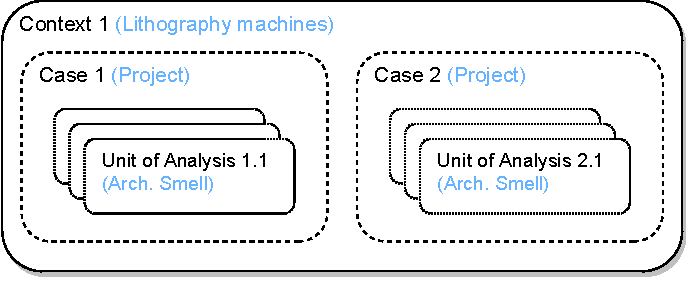
\includegraphics[width=.7\textwidth]{c4/Fig2.pdf}
    \caption{The case study design using Runeson et al.'s representation \cite{Runeson2012}.}
    \label{c4:fig:case-design}
\end{figure}

The five stated research questions require different types of data in order to be answered.
RQ1, RQ2, and RQ3 necessitate \emph{quantitative} data about architectural smells extracted from multiple versions of the source code of each project.
RQ4 and RQ5, instead, require \emph{qualitative} data collected from software architects and engineers working on the studied projects.
The remainder of this section explains how the data collection for these two groups of research questions was performed.

\subsubsection{Quantitative data collection}
\paragraph{Projects and Architecture}
The first step of performing \emph{quantitative} analysis is selecting the cases to analyse. 
The selection of the projects was done in consultation with an architect from the company. We requested that the list of projects would differ as much as possible in terms of total number of lines of code (LOC), to maximise the diversity in our sample.
The selection was also influenced based on the interest of the architects responsible for each project in obtaining information regarding the presence of architectural smells in their systems.
The final list of projects is shown in Table \ref{c4:tab:projects}.
The projects differ greatly in total number of lines of code analysed, from a few thousands to a few million. Each project is also responsible for a single step in the manufacturing process of the microchip.
One project (P09) is relatively new compared to the rest, and thus smaller both in terms of LOC and number of versions.
We also note that, over time, the company has split projects in two or more parts to better manage them, causing both a steep decrease in the LOC of some projects, and other projects starting with a high number of lines of code.

It is important to mention a few details about the architectural style of the projects selected. 
The company adopts a layered architectural style with each project (ideally) only communicating with projects from layers below them or from the same layer.
Each project is divided into multiple clusters of components that handle a specific functionality provided by that project. Larger projects may be divided into multiple teams, each maintaining their own cluster of components.
Projects situated in higher layers provide functionality that allow the user to command the machine and configure it.
In contrast, projects located in lower layers are responsible to govern the hardware, orchestrate other components, and provide abstraction layers to allow the deployment of the code on different kinds of hardware.
Finally, we note that all projects contain both C and C++ files, with the former type being the most popular one. 

\begin{table}[tbp]
    \footnotesize
    \centering
    \caption{The list of projects analysed in this study. MLOC = Million Lines Of Code}
    \label{c4:tab:projects}
    \begin{tabular}{@{}llll@{}}
    \toprule
    \textbf{ID} & \textbf{Description} & \textbf{Versions analysed} & \textbf{MLOC last version} \\ \midrule
    P01  & Reticle handling     & 31        & 4.88         \\ % FC-002
    P02  & Waterflow control    & 37        & 3.92         \\ % FC-003
    P03  & Dose control         & 37        & 1.58         \\ % FC-009
    P04  & Light control        & 37        & 2.22         \\ % FC-010
    P05  & Immersion control    & 37        & 0.86         \\ % FC-015
    P06  & Device \& Data subsystems & 37    & 6.45         \\ % FC-025
    P07  & Machining control    & 37        & 2.56         \\ % FC-028
    P08  & Input data manager   & 18        & 2.31         \\ % FC-042
    P09  & Alignment \& Diagnostics & 9     & 0.011      \\ % FC-086
    \bottomrule
    \end{tabular}
\end{table}

\paragraph{Architectural Smells Detection}
The analysis of the projects included the following phases: detection of architectural smells, the tracking of architectural smells over time, and the calculation of the software metrics necessary for the data analysis. 
The detection-tracking process is repeated for every version available and the results are merged at the end of the whole process.

To detect AS, we extended \textsc{Arcan} to support the proprietary C/C++ used by the company participating in this study. 
\textsc{Arcan}'s results were validated by previous studies and obtained a precision ranging from 70\% to 100\% \cite{Arcelli2020,Arcelli2017}.
The detection of smells is carried out through the a dependency graph (DG) created by \textsc{Arcan} given the source files of a C/C++ or Java project.
The DGs of these two languages, however, present several differences that influence the architectural smell detection process.
For example, DGs for C/C++ projects have nodes and edges that respectively represent and connect header files, which are obviously not present in DGs of Java projects.
Moreover, the package structure of Java projects is a tree structure that requires dependencies to propagate from the leaves (i.e. the classes) to their parents (i.e. the packages containing those classes, the packages containing those packages, and so on).
In ASML, however, there is no such concept and there are no child components.
The different structures of these two languages (or, more technically, the different graph schemas) imply that dependencies are constructed differently: in the case of this study, the detection of architectural smells was tailored based on the guidance of ASML engineers.
In particular, components were treated as packages and header files as Java interfaces, but only for the purpose of mining dependencies (i.e. headers were not considered for smell detection).
All the dependencies detected in the header files were carried over to the exact files implementing, or using, those dependencies.

Note that, in order to extract the dependency graph, we had to write specific code that would account for all the proprietary changes the company implemented to their compiler, and consequently to the syntax of the code. 
Additionally, since some of the files were automatically generated at compile time, we were also required to compile the projects in order to pick up as many dependencies as possible. These files contained dependencies between internal components that were manually declared by the engineers in a proprietary file format, and missing these dependencies would have eventually resulted in incomplete results.
These two tasks turned out to be very time-consuming, and packed with arduous technical challenges.

The tracking of the smells is then done using \textsc{ASTracker} (see Chapter \ref{chap:2}), which matches smell instances from two adjacent versions that correspond to the same smell (i.e. they affect the same files but in adjacent versions).
Usually, this process is susceptible to file renamings; however, the file naming policies of the company prevented the introduction of noise in this part of the analysis, as file renamings are not an encouraged practice.

The versions we analysed were all the snapshots of the projects that the company tagged as \emph{releases} in their version control system (VCS). The time period taken into consideration is 3-years long (from 2017 to 2020) and each release took place, on average, 35 days after the previous. Note that the we stopped at 3 years because the VCS used by the company at the moment was adopted 3 years before the start of this research.

A detailed representation of the whole data collection process is shown in Figure \ref{c4:fig:data-collection-process}.
For each version in the VCS, we compiled the source code to obtain the automatically generated files (omitted from Figure \ref{c4:fig:data-collection-process}), then we ran \textsc{Arcan} on each project to obtain the dependency graph of that version.
At the end of the analysis, we ran \textsc{ASTracker} to synthesise the information contained in the dependency graphs into CSV files of raw data. These files were then processed to create the datasets for each individual research question.

\begin{figure}
    \centering
    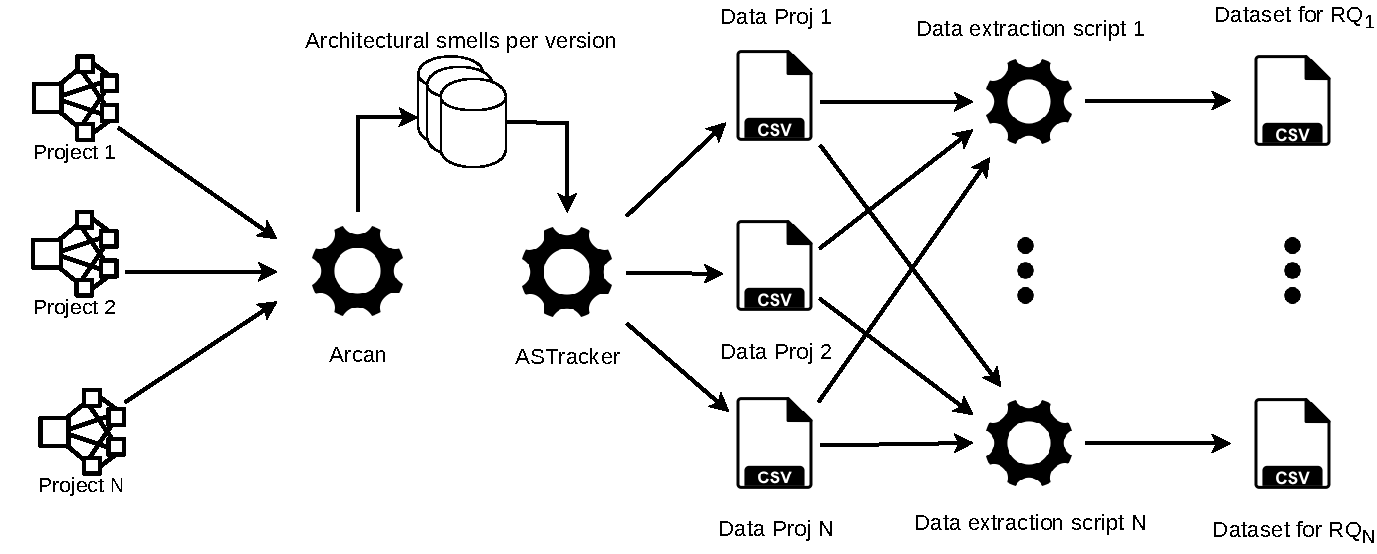
\includegraphics[width=1\linewidth]{c4/Fig3.pdf}
    \caption{Quantitative data collection process.}\label{c4:fig:data-collection-process}
\end{figure}

\subsubsection{Qualitative data collection}
While RQ1, RQ2 and RQ3 required the \emph{quantitative} data described in the previous sub-section, RQ4 and RQ5 required \emph{qualitative} data to be fully answered. 
To this end, we planned a series of \textbf{interviews} with the engineers and architects working on the projects we analysed.

The process for selecting the participants to our interviews started with a presentation of our analysis in one of the monthly meetings between all the architects of the company.
Architects that showed interest were contacted and their projects were analysed. 
Afterwards, we prepared an interactive report\footnote{An anonymised version is available in the replication package of this study.} specific to each project analysed and sent it to the corresponding architect.
Each architect was then asked to pick a handful (3-5) of engineers that we could interview; they were also asked whether they would like to take part in the interview themselves.
Each participant received a consent information letter, informing them of their rights as participants, and a copy of the report with the results of the analysis. The report also contained a quick guide to allow them to understand the results. The participants were asked to inspect the report before taking part in the interview. 

The interviews lasted 30 to 40 minutes each and were performed remotely by the first author using video-conferencing, individually with each participant listed in Table \ref{c4:tab:participants}.
Interviews followed a semi-structured format \cite{Runeson2012} as depicted in Figure \ref{c4:fig:interview-phases} and further detailed in Figure \ref{c4:fig:interview-questions-sub-phases}.
As it can be noted, the actual questioning session (Phase 2, in Figure \ref{c4:fig:interview-phases}) was preceded by an introduction to the study, some demographic questions, and an explanation of the key theoretical concepts necessary to understand the questions in Phase 2.
The questions asked in Phase 2, were grouped by topic and map to either RQ4 or RQ5, as shown in Figure \ref{c4:fig:interview-questions-sub-phases}.
Given the semi-structured format, the interviewers also asked follow-up questions and may have not followed the predefined list of questions if an interesting point, worth of further investigation, was touched during the session.
The full interview guide is available in Appendix \ref{c4:appendix:interview-guide}.

\begin{figure}
    \centering
    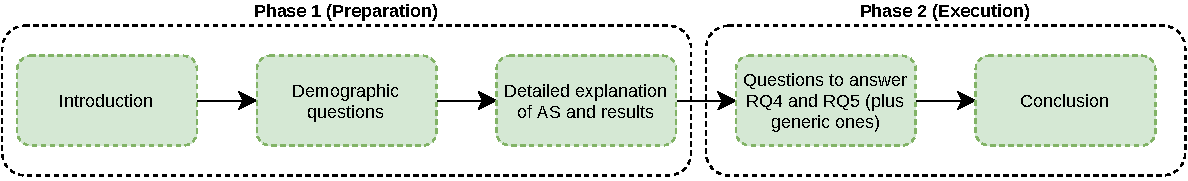
\includegraphics[width=1\linewidth]{c4/Fig4.pdf}
    \caption{The phases and structure of the interviews.}\label{c4:fig:interview-phases}
\end{figure}

\begin{figure}
    \centering
    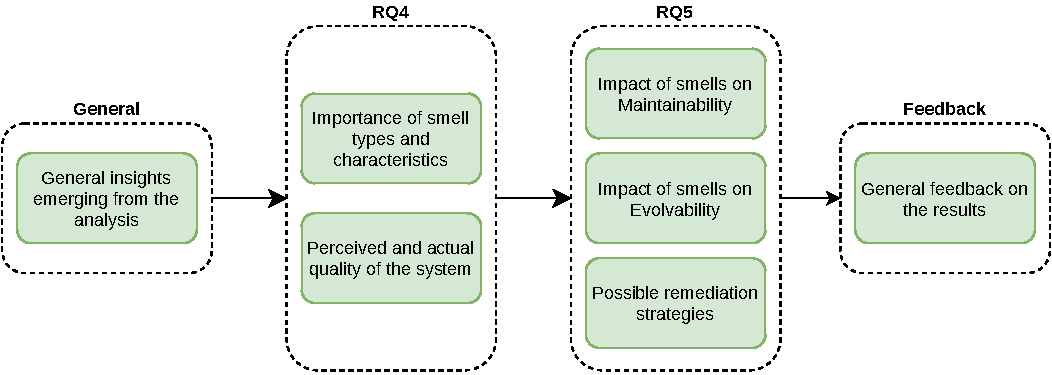
\includegraphics[width=1\linewidth]{c4/Fig5.pdf}
    \caption{The structure of the first step of phase two, focusing on RQ4 and RQ5.}\label{c4:fig:interview-questions-sub-phases}
\end{figure}

\begin{table}[tbp]
    \centering
    \caption{Background information on the interviewee and their respective projects.}
    \label{c4:tab:participants}
    \begin{tabular}{@{}clm{4cm}cc@{}}
        \toprule
        \multirow{2}{*}{\bfseries ID} & \multirow{2}{*}{\bfseries Project} &\multirow{2}{*}{\shortstack{\bfseries Official position}} & \multicolumn{2}{c}{\bfseries Years of exp.} \\
        &  &  &\multicolumn{1}{c|}{\bfseries curr. role} & \textbf{in total} \\ \midrule
        I0 & P05 & Product Architect & 4 & 8 \\    % p1_uu
        I1 & P03 & Design Engineer & 3 & 4 \\    % i1_gl
        I2 & P03 & Software Architect & 8 & 14 \\   % i2_gj
        I3 & P03 & Design Engineer & 4 & 15 \\   % i2_sl
        I4 & P03 & Design Engineer & 2 & 8 \\    % i4_jm
        I5 & P08 & Design Engineer & 4 & 10 \\   % i5_js
        I6 & P08 & Software Architect & 6 & 15 \\   % i6_vj
        I7 & P07 & Software Architect & 7 & 25 \\   % i8_as
        I8 & P07 & Software Architect & 8 & 22 \\   % i9_mb
        I9 & P07 & Software Architect & 6 & 23 \\   % i10_dh
        I10 & P02 & Design Engineer & 3 & 3 \\   % i11_xh
        I11 & P02 & Lead Design Engineer & 5 & 20 \\  % i12_rn
        \midrule
    \multicolumn{3}{l}{\textit{\textbf{Average}}} & 5 & 13.9 \\ \bottomrule
    \end{tabular}
\end{table}

\section{RQ1 -- Architectural smells evolution}\label{c4:sec:rq-1}
\subsection{RQ1.1 -- Evolution of smell characteristics}\label{c4:sec:rq1.1}
\subsubsection{Data analysis methodology: Dynamic Time Warping}\label{c4:sec:methodology-rq1.1}
To understand how smell characteristics evolve over time, we adopt the same technique we used in Chapter \ref{chap:2} \cite{Vaucher2009}: signal classification with Dynamic Time Warping\footnote{The implementation used for this analysis was provided by the R package \texttt{dtw}.} (DTW) \cite{Kruskal1983}.
This approach considers every series of values of every characteristic of every smell instance as a signal (or time series) and then compares each signal to a series of predefined signals (templates), each one with a corresponding label. 
Depending on the template that is the mathematically closest to the signal, a label is assigned to it.

Formally, we can model the problem as follows: for every smell characteristic $C^{k}$ of a certain smell $k$ we consider the different values $C^{k}_i$ as a signal $S$. We then compute the following variables: $h = \max S$; $l = \min S$; and $m = (h+l)/2$.
These three values are then used to build the seven templates, named from $a$ to $g$, shown in Figure \ref{c4:fig:classification-templates}. For example, template (c) is defined as $c = (l, l, h, h)$.
The values $l$, $m$, $h$ are re-calculated for each signal classified.
Finally, the signal is classified by comparing the distance of the signal from each template, and selecting as a label the name of the closest template. 

\begin{figure}[h]
    \centering
    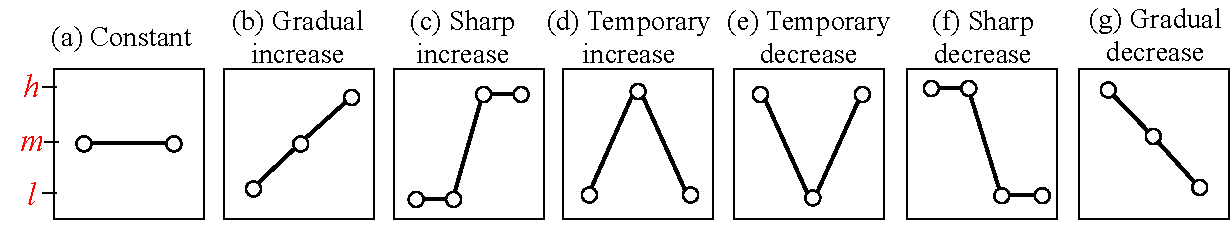
\includegraphics[width=0.9\textwidth,trim={0.2cm 0 0 0},clip]{c4/Fig6.pdf}
    \caption{Trend evolution classification templates. Figure adapted from the work of Vaucher et al. \cite{Vaucher2009}.}\label{c4:fig:classification-templates}
\end{figure}

Even though the selected templates offer a good variety of possible signal shapes, there exist some cases that may not be well approximated by the current selection.
One example is a signal that varies between two integer values (e.g. 6-7) multiple times, which would be classified by the model as a constant signal (i.e. template (a)).
Nonetheless, we deem that the approximation offered by the model when classifying such unusual signals, is sufficient for the purpose of this chapter for the following reasons:
\begin{itemize}
    \item the templates selected represent simple and general cases, thus they simplify interpretation and analysis;
    \item a signal is classified based on the distance DTW calculates between the points from the template and points from the signal, thus the classified signal has at least an internal component that resembles the assigned template.
\end{itemize}

\subsubsection{Results}\label{c4:sec:results-rq1.1}
The results shown in this section concern smells that affected the system for at least 3 releases, in order to avoid spurious outcomes and focus on long-lived smells. Note that in this section, unless specified, or the context implies otherwise, when we refer to an AS instance we usually mean a smell that was detected in multiple versions and was identified as the same smell.

Finally, we use the following terminology: \emph{version} and \emph{release} are used interchangeably, \emph{component} refers to a group of files defined as such by the architects of the system, \emph{artefact} refers to both files and components, and the terms \emph{co-occurrence} and \emph{overlap} (among AS) are used interchangeably.

\begin{table}[tbp]
    \centering
    \caption{The number of unique temporal AS instances that that have an age of at least 3.}
    \label{c4:tab:smell-count}
    \begin{tabular}{@{}lcc|c@{}}
    \toprule
    \textbf{Smell Type} & \textbf{File-level} & \textbf{Component-level} & \textbf{Total} \\ \midrule
    Cyclic Dependencies & 14637 & 941 & \textbf{15578} \\
    Hublike Dependencies & 151 & 40 & \textbf{191} \\
    Unstable Dependencies & -- & 273 & \textbf{273} \\
    God Component & -- & 190 & \textbf{190} \\ \bottomrule
    \end{tabular}
\end{table}

\begin{figure}[h]
    \centering
    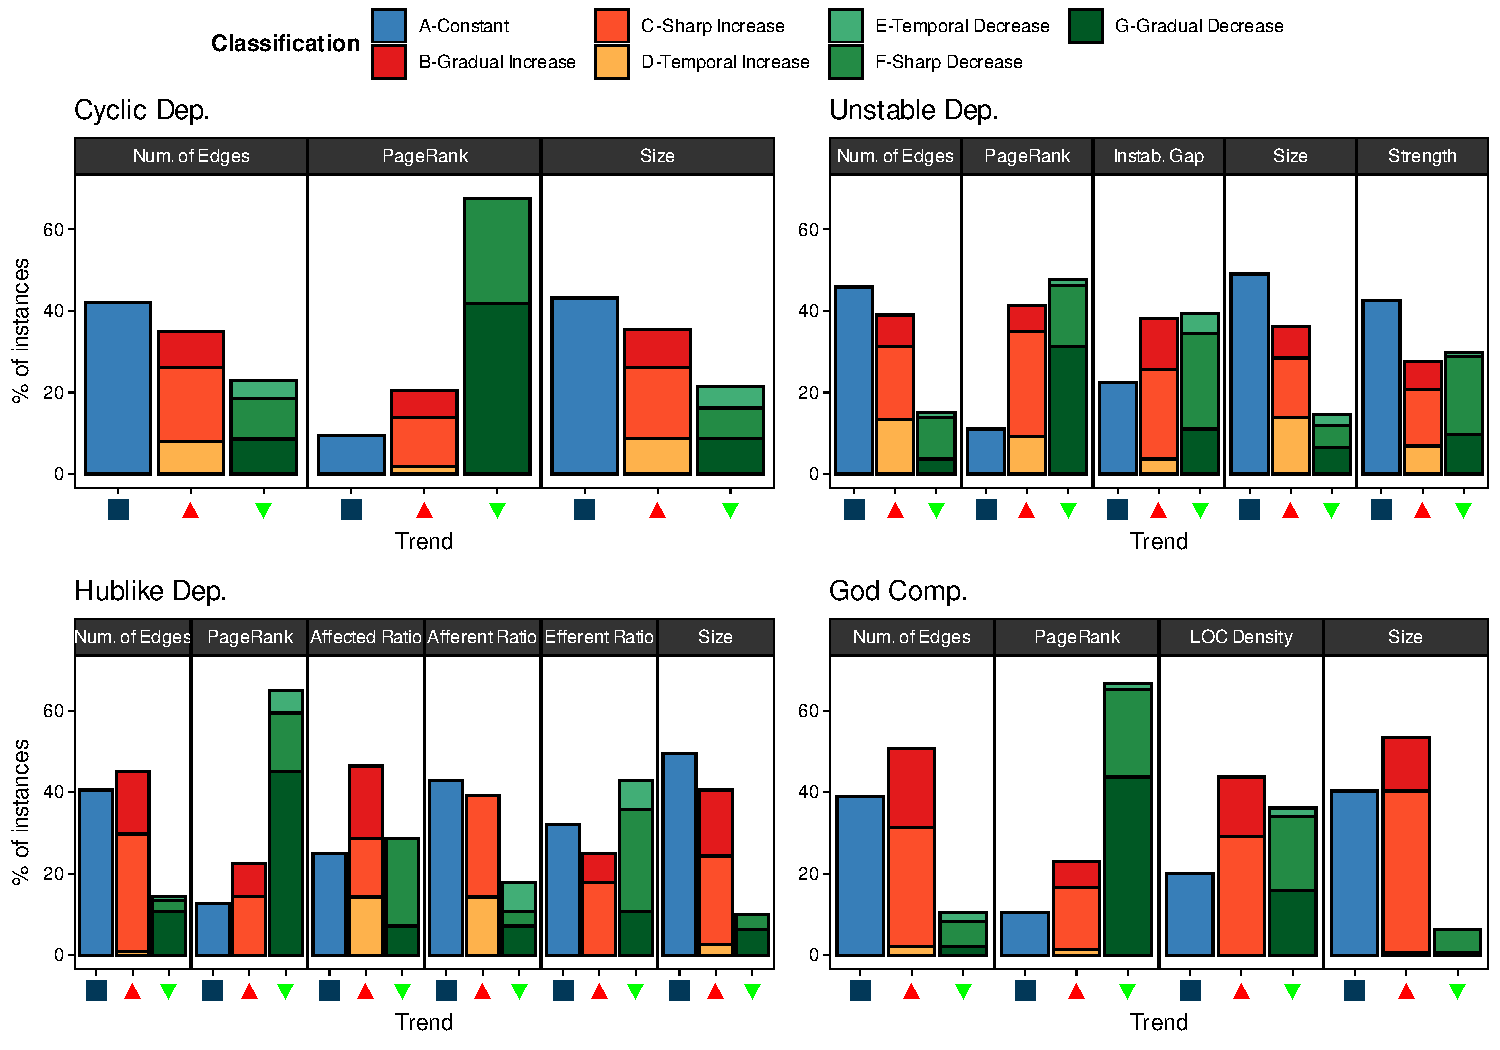
\includegraphics[width=\textwidth]{c4/Fig7}
    \caption{The classification of AS's instances trend for various characteristics grouped by smell type. The classification is in percentage of the total number of instances with at least an age of 3. The classification (represented by the colour) for each characteristic is grouped by the overall trend (constant, represented as a black block; increasing, represented as an up-pointing triangle; and decreasing, represented by a down-pointing triangle).}\label{c4:fig:dtw-classification}
\end{figure}

\paragraph{Cyclic Dependencies (CD)} As Figure \ref{c4:fig:dtw-classification} shows, most of the 15578 CD instances exhibit either an increase in the number of artefacts affected (i.e. size) or they remain steady over time. More specifically, 43\% increase in size in some way, 36\% stay constant, and only 21\% of them decrease. As expected, a similar pattern also emerges when looking at the number of edges among the affected artefacts (since they are correlated , see Chapter \ref{chap:2}).

The PageRank of the cycles\footnote{Calculated as the maximum PageRank of the affected artefacts and normalized by the number of artefacts in a version.} is decreasing in 70\% of the instances, contrary to what we found in a previous study on open source Java systems from Chapter \ref{chap:2}.
The remaining 21\% of instances increase in PageRank, and only 9\% stay constant.

Typically, a file can have two types of dependencies (internal to the system), the first is to another file in the same component, and the second is to a file in another component.
Dependencies that cross the border of the component can also create cycles among components, either a) directly as a result of two or more files from the affected components creating a cycle among them; or b) indirectly, as a result of files that depend on files in another component but do not create a cycle among them, yet they create the dependencies among the components that in turn create the cycle (see Figure \ref{c4:fig:package-cycles}). We call this characteristic `Affected design level' (see Table \ref{c4:tab:characteristics}), and we used this characteristic to study how many cycles cross this border.
In the systems we analysed, 98\% of cycles are only among files, whereas the remaining 2\% are at the component level.
This means that, the vast majority of cycles is fully enclosed within the component their files belong to (i.e. they do not cross the component's border), which is a good sign of encapsulation but also means that \textbf{components are quite entangled internally}.
This could probably be because of the specific architecture of the system, which is divided in components that hide all the functionality under an interface.

\begin{figure}
    \centering
    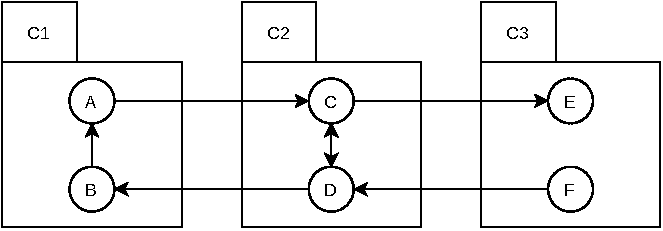
\includegraphics[width=0.5\textwidth]{c4/Fig8}
    \caption{Example of two cycles among components: one among $C1$ and $C2$ that is also present among the files contained in them; and one among $C1$, $C2$ and $C3$ that is only present among the components. Figure adapted from \cite{AlMutawa2014}.}
    \label{c4:fig:package-cycles}
\end{figure}

Concerning the shape of the cycles, 73\% of the instances exhibit no change in shape over time, whereas the remaining ones (4206 instances) mutate as illustrated in Figure \ref{c4:fig:chord-shapes}.
The chord diagram depicts the proportion of the cycle shapes that changed into another shape. Each sector of the diagram corresponds to a specific shape with outgoing edges that represent the proportion of the population of that shape that transforms into another shape. For example, only a tiny percentage of circle instances change shape, and therefore the corresponding sector of the circle shape is rather small, despite constituting the majority of the population of cycles (86\%).
As it can be noted, some shapes (i.e. chain and star) are more prone to changes than others, i.e. they have a greater percentage of their population changing.
There is also a certain balance across all shapes in the number of instances changing \emph{into} a shape and changing \emph{from} a shape. By looking more closely at the data, we notice that this was due to the fact that most instances bounce back and forth from one shape to the other.
The circle is a special case: despite only 5\% of circle instances being involved in changes, due to the sheer number of circle instances, the majority of changes involve circle shapes. Thus, circles are more likely to transform into any other shape, unlike stars for instance, which are more likely to change into chain or circle only.

\begin{figure}
    \begin{subfigure}[t]{0.65\textwidth}
        \centering
        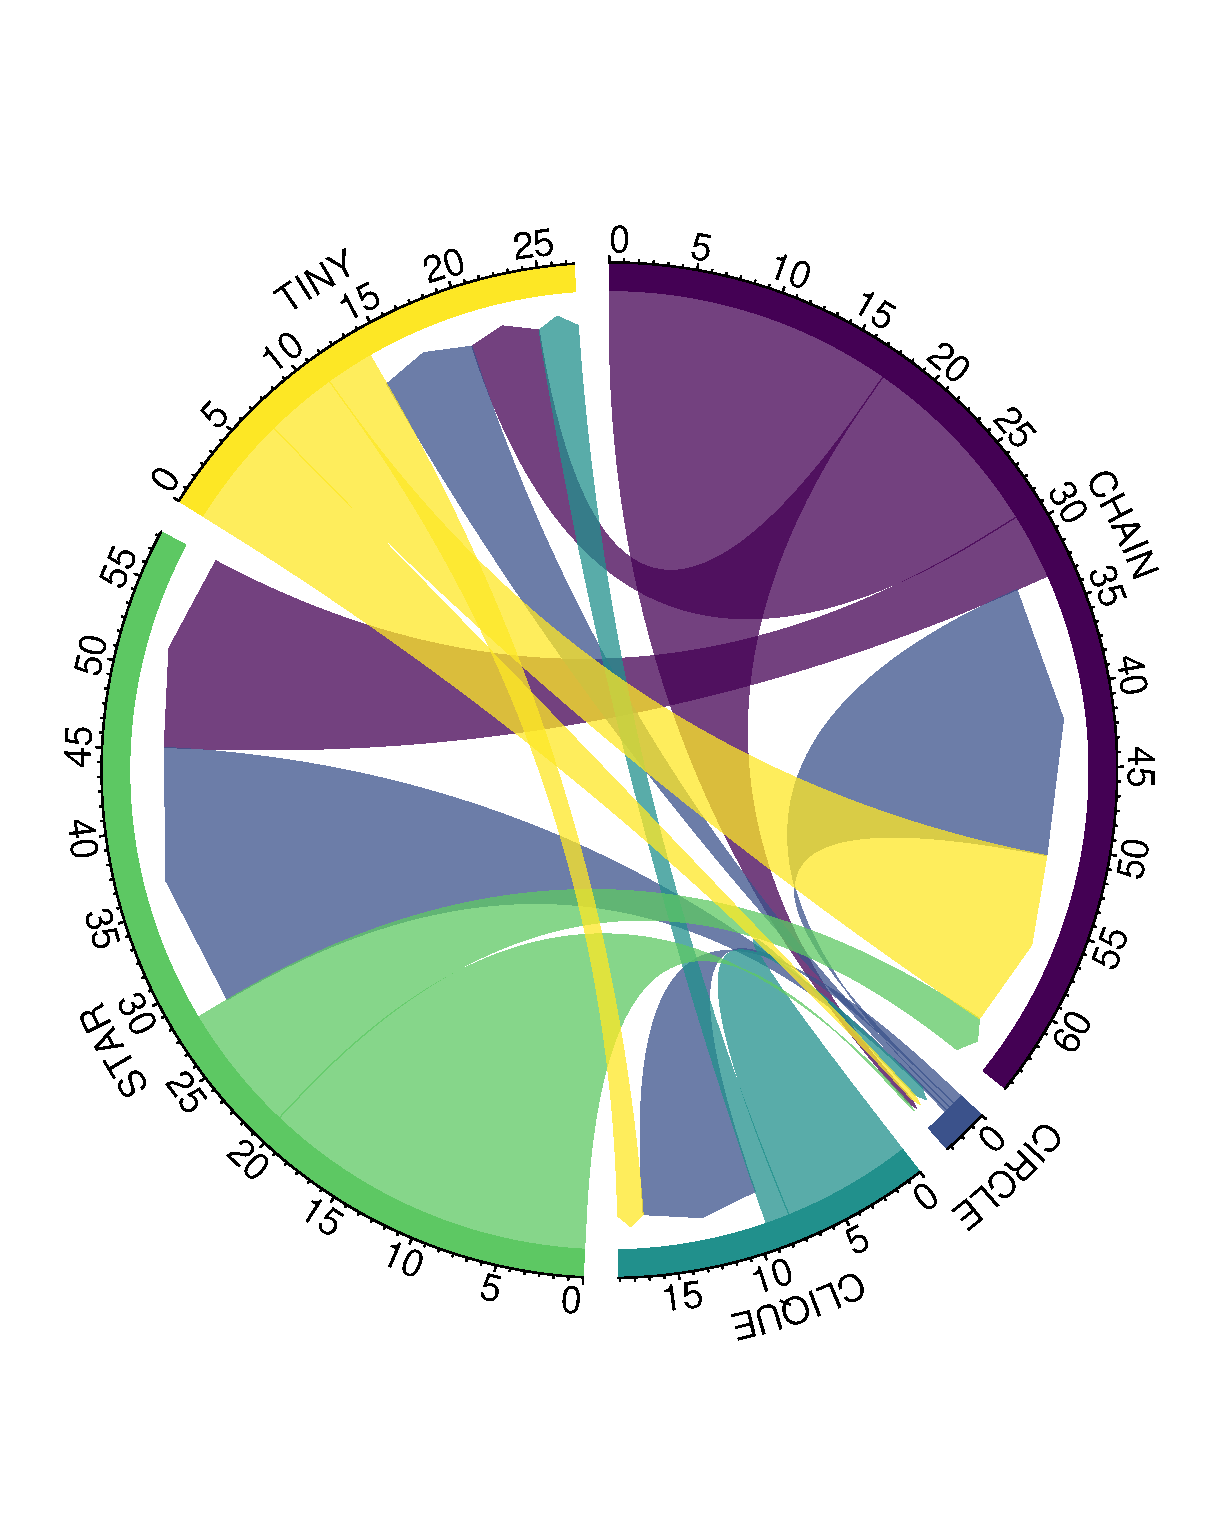
\includegraphics[clip, trim=0cm 3.2cm 0cm 3.8cm,width=0.7\textwidth]{c4/Fig9a}
        \caption{Chord diagram of how cycle shapes change, controlled for the distribution of shapes in the cycles population. The numbers represent the percentage of the total population of the corresponding shape.}\label{c4:fig:chord-shapes}
    \end{subfigure}
    \hfill
    \begin{subfigure}[t]{0.3\textwidth}
        \centering
        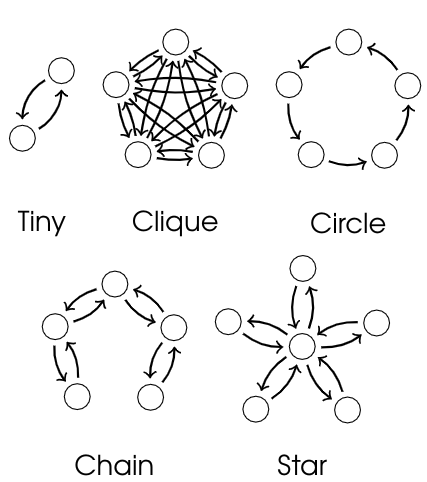
\includegraphics[width=\textwidth]{c4/Fig9b.png}
        \caption{Symmetric cycle shapes detected by \textsc{Arcan} and defined by Al Mutawa et al. \cite{AlMutawa2014}.}\label{c4:fig:cycle-shapes}
    \end{subfigure}
    \caption{The cycle shapes considered in this study and how they change over time. The total  population of cycles is as follows: Circle 86\%, Clique 7\%, Tiny 4\%, Chain 1.5\%, Star 0.5\%). Only instances that persists for at least 3 releases are considered.}
\end{figure}

\paragraph{Unstable Dependencies (UD)} For this smell type, as shown in Figure \ref{c4:fig:dtw-classification}, 49\% of the 273 instances tend to remain constant in size over time, in 37\% of the cases UD increase in some way and the remaining 14\% of the times they experience a decrease of some sort. A similar behaviour is observed for the number of edges as well.

The PageRank of UD differs quite a lot from the other smell types, as we observe that 11\% of instances stay constant, 42\% have an increase of some sort, and 46\% experience a mostly gradual decrease. 
For other smell types, PageRank is mainly decreasing, whereas for unstable dependencies, a significant amount of instances exhibit an increase, meaning that they move towards more central parts of the system.
This means that components that are prone to change move towards more inner parts of the system.
This is not an ideal scenario, as Martin \cite{Martin2018} states that it is preferred to have dependencies that point toward more stable components in order to reduce change propagation.

Moreover, the gap in instability between the affected component and its dependencies is showing an increase in 38\% of instances, a decrease in 39\% of instances, while the remaining 22\% exhibit a constant trend. 
This means that there is no clear trend of instances that exhibit a clear increase, or decrease, in the instability measured in the central component and in its less stable dependencies (see Figure \ref{c2:fig:ud} for more context).

The ratio of dependencies of an UD-affected component that are less stable than the affected component (i.e. the strength characteristic) was found to increase or decrease in equal percentages (28\% each), and stay constant in the remaining of cases (42\%).

\paragraph{Hublike Dependency (HL)} Hubs tend to either stay constant in size (49\% of instances) or increase (40\% of instances), with the remaining 11\% decreases.
Therefore, over time, hubs involve more and more artefacts.

By looking at the number of files within the central component that provide functionality to external components (incoming dependencies, i.e \emph{afferent ratio}\footnote{This is a ratio characteristic, however, for this analysis, it was weighted with the number of elements in the central artefact in the respective version to ensure we detected the absolute variations inside the internal artefact.}) and at the ratio of files within the central component that use external components (outgoing dependencies, i.e. \emph{efferent ratio}) we note the following: the afferent ratio is increasing in 46\% of instances and decreasing in 11\% of instances only (remaining 43\% are constant); the efferent ratio on the other hand, exhibits an increase in 32\% of instances and a decrease in 36\% of instances (remaining 32\% are constant).
This means that at least \emph{some} HL instances tend to provide more functionality over time themselves rather than depending on their outgoing dependencies to provide such functionality.
This phenomenon is not optimal for the overall architecture of the system as it means that hubs, over time, \emph{replace} the functionality of their dependants: instead of having other dedicated components to provide that functionality, hubs take their place (i.e. they accumulate features).
The final result of this process is that hubs drift away from their initial purpose and become aggregators of functionality, weakening the separation of concerns originally intended by the architects. %This point should probably be moved to the discussion with a forward reference here.

Finally, we observe the trend of the \emph{affected ratio}, i.e. the number of files within a hublike component that create the incoming and outgoing dependencies, thus creating the smell. This is increasing in 46\% of the cases, decreasing in 29\% of cases, and the remaining 25\% are constant.
Thus, as aforementioned, hubs grow to become more complex over time and more connected to their incoming and outgoing dependants.

\paragraph{God Component (GC)} The number of elements in the components affected by GC (i.e. size) increases in 53\% of the cases, stays constant in 40\% of the cases and decreases in 6\% of the cases.
Similarly, also the lines of code density increases 46\% of times, decreases in 34\%, and stays constant in the remaining 20\%.
We can therefore conclude that GC tend to grow in size over time, possibly aggregating more concerns and growing in complexity.

The PageRank of GCs follows a similar pattern as for the other smells, with 65\% of instances exhibiting a steady decrease, 24\% of them an increase, and the rest of them (11\%) stay constant.
This is a rather unexpected result as GCs, being large components by definition, are expected to also have an increase in their centrality over time.
This result however hints that the new functionality added in other parts of the system is ultimately less and less connected to the functionality offered by GCs given the decreasing PageRank of the majority of GC-affected components.
Such a pattern however is only observed globally in the whole dependency network of the system; locally, GCs still experience a growth in the number of files within the component and number of dependencies among those files (as mentioned above).

\paragraph{Summary of RQ1.1 results}
The general trend that we notice across the evolution of the smell characteristics is that each characteristic fits one of two patterns: it either (1) exhibits a \emph{dominant constant} trend followed by either an increasing or decreasing trend; or (2) it exhibits a \emph{dominant increasing} or \emph{decreasing} trend. 
The first case entails that those smell characteristics are mostly unaffected by the evolution of the smell. Examples of this case are CD Size, UD Size and CD Number of Edges.
In the second case, the opposite is true and the evolution of smell characteristics has a clear direction over time. Example of this case are PageRank for all smell types or GC Size.
This information can be exploited by using the smell characteristics of the second type as predictors for the evolution of an instance to establish the severity of a smell.
Instances with smell characteristics that have a clear trend and are bound to reach certain thresholds could be brought to the attention of developers before they become problematic and pose a greater threat to the maintainability and evolvability of the system.

\subsection{RQ1.2 -- Persistence of Architectural Smells in the system}
\subsubsection{Data analysis methodology: Survival analysis}
Different architectural smell types were found, in Chapter \ref{chap:2}, to have drastically different persistence rates within Java Open Source Systems.
To establish the persistence rates in our case (embedded systems written in C/C++), we employed the same technique used in our previous work in Chapter \ref{chap:2}: the Kaplan-Meier estimator, or survival analysis.
This technique is typically used in the biomedical sciences and in product reliability assessment; in addition, prior to our previous work from Chapter \ref{chap:2}, it was also employed in software engineering to analyse code smell persistence \cite{Chatzigeorgiou2014}.

Unlike simple descriptive statistics, such as mean or density functions, survival analysis also takes into consideration the possibility that a smell continues to affect the system even after the last version included in the analysis.
In the biomedical domain, this event is associated with the patient surviving past the period of the analysis.
More technically, this type of data is said to be \emph{right-censored}, because the outcome of the treatment cannot be measured, due to the conclusion of the study.

The survival analysis is performed using the Kaplan-Meier estimator \cite{Kaplan1958}, a non-parametric statistic that estimates the survival probability of a type of smell as the system evolves (new versions are released).
The statistic gives the probability $p$ that an individual patient (i.e. smell in our case), will survive past a particular time $t$.
At $t = 0$, the Kaplan-Meier estimator is equal to 1, and as $t$ goes to infinity, the estimator goes to 0. Also, the probability of surviving past a certain point $t$ is equal to the product of the observed survival rates until $t$.

\subsubsection{Results}
The results of this analysis are presented in Figure \ref{c4:fig:survival-analysis}. The figure shows the survival rate for both smell types and cycle shapes.
Figure \ref{c4:fig:survival-smells} differentiates between smells at file and component level for cycles and hubs: the appearance and disappearance rates of dependencies among files and dependencies among components may be different, thus we study them separately.
Given their definitions, UDs and GCs cannot be detected at file level; therefore, we only considered them at component level.

\paragraph{Smell types}
By looking at Figure \ref{c4:fig:survival-smells}, one can note that the smell type with the lowest survival rate are cyclic dependencies among components, which tend to disappear from the system rather quickly: they exhibit a 50\% probability of surviving more than 6 versions. 
Cycles at file level instead manage to affect the system for a little bit longer, reaching 50\% probability of surviving after 9 versions. This makes sense as it is much more likely for developers (in the company subject to this study) to eliminate unwanted dependencies towards files in external components, rather than towards internal files.
Hubs show a similar survival rate and reach the 50\% probability of surviving at 8 versions, at file level, and 16 versions at component level, before converging later on.
God components and Unstable dependencies reach it at 19 and 24 versions, respectively.
God components, however, maintain a flatter curve and stay close to the 50\% threshold for longer.
Another interesting fact that can be derived from Figure \ref{c4:fig:survival-smells} is that the curves stabilise eventually (see the right-most part of the plot) and do not go below a certain probability (excluding cycles at component level).
This is probably due to the fact that the parts of the system affected by smells for a long time tend to become legacy code that is either very hard to change or has no reason to be changed. Our interviews have provided some insights into this phenomenon, which we will explore in more depth in the discussion section (Section \ref{c4:sec:discussion}).

\paragraph{Cycle shapes}
In Figure \ref{c4:fig:survival-shapes}, we focus on the survival rates of cyclic dependencies, regardless of the type of artefact they affect, and distinguish between different shapes.
Circles are the ones that are more likely to disappear from the system (50\% chance of surviving for one version), however, they are also the most common type of shape and much easier to form, especially in comparison with chain, clique and star.
Cliques, despite being a much more complex type of shape, have a similar survival rate to the one we observed for circles.
This is probably due to the fact that cliques are less common, harder to appear, and can be ``broken'' just by removing one edge from their structure.
Moving to stars, despite being relatively complex (and thus relatively easy to break down), they manage to survive within the system for a much longer time, reaching 50\% of survival probability only after 17 versions.
Finally, chain and tiny shapes are the ones that exhibit the longer survival rate while also having a relatively stable curve.
This is probably because: a) these shapes are very similar; b) cycles between fewer elements are less likely to be perceived as problematic - in fact, they could be intentional.

\begin{figure}
    \begin{subfigure}[b]{0.49\textwidth}
        \centering
        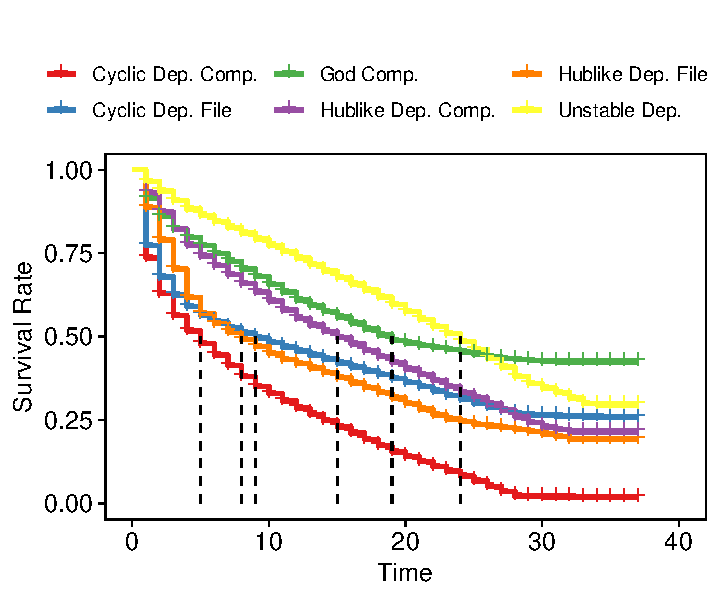
\includegraphics[width=\textwidth]{c4/Fig10a}
        \caption{Survival rate of smell types.}\label{c4:fig:survival-smells}
    \end{subfigure}
    \hfill
    \begin{subfigure}[b]{0.49\textwidth}
        \centering
        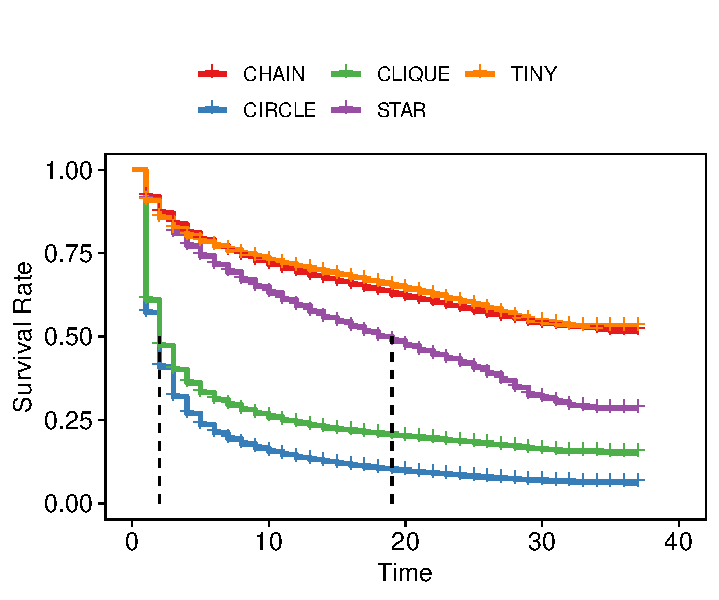
\includegraphics[width=\textwidth]{c4/Fig10b}
        \caption{Survival rate of cycle shapes.}\label{c4:fig:survival-shapes}
    \end{subfigure}
    \caption{A visualisation of the Kaplan-Meier estimators. The plot reads as follows: after a certain time $t$ (on the $x$ axis), smell type $s$ has a probability $p$ (on the $y$ axis) to survive. Dashed vertical lines represent the value $t$ when $p = .5$.}
    \label{c4:fig:survival-analysis}
\end{figure}


\section{RQ2 -- Architectural smells co-occurrence}\label{c4:sec:rq2}
\subsection{Data analysis methodology}\label{c4:sec:methodology-rq2}
To find out what pairs of architectural smells co-occur more often, we used a simple approach: we calculated the co-occurrence matrix for each type of architectural smell detected by \textsc{Arcan}. This resulted in a $6\times6$ matrix, where the rows and columns are labelled with the names of the smells. However, for the sake of readability, we report the results in two matrices, one $4\times4$ matrix for component-level smells and one $2\times2$ matrix for file-level smells. 
The value in each cell of these two matrices is calculated as follows: 
\begin{equation}
    cooc_{i,j} = \frac{\# \textnormal{ of instances of type } i \textnormal{ overlapping one of type } j}{\# \textnormal{ of total instances of type } i} \times 100
\end{equation}
with $i \neq j$.
By `overlapping' we mean that the two smell instances must affect at least one artefact in common in the same version.
However, some architectural smells involve various artefacts which play different roles; thus we also distinguish between the different parts of the smell that may overlap:
\begin{itemize}
    \item for Hublike Dependencies we distinguished between the incoming dependencies (artefacts C1-3 in Figure \ref{c2:fig:hl}), outgoing dependencies (artefacts B1-3 in Figure \ref{c2:fig:hl}), and the central component, or the hub (artefact A in Figure \ref{c2:fig:hl});
    \item for Unstable Dependencies we distinguished between the central component (component A in Figure \ref{c2:fig:ud}) and its outgoing dependencies that are less stable (components B1-3 in Figure \ref{c2:fig:ud});
    \item for Cyclic Dependencies we did not make any distinction, as every component of the cycle plays a similar role in the smell;
    \item for God Component we did not make any distinction as the smell constitutes a single element.
\end{itemize}

Note that for this analysis, we counted every smell detected individually, \emph{without} linking it to its corresponding instances in adjacent versions. This way, we capture not only the overlaps that take place in multiple versions but also those that happen in one version; thus we represent a more precise picture of the overlaps of smells. Moreover, this approach is very similar to what was done in a previous study on code smells \cite{Palomba2018}.

\subsection{Results}\label{c4:sec:results-rq2}
The results obtained for this research question are reported in Table \ref{c4:tab:co-occurrence}, for component-level smells, and in Table \ref{c4:tab:co-occurrences-files} for file-level smells.
The values in the table represent the percentage of the total number of instances of the smell in the corresponding row that overlap with the smell in the corresponding column (hence the table is not symmetrical).

\paragraph{Component-level smells}
With a first glance at Table \ref{c4:tab:co-occurrence}, one can note that the architectural smells in the analysed systems have a very high overlap, which is reasonable given the definition of some smells (i.e. they involve numerous components).

Looking at the CDs in Table \ref{c4:tab:co-occurrence}, we note that given their abundant presence in the system, they overlap with the other smell types in high percentages (from 76\% to 99\%, as seen in the first row). 
This is most likely due to the fact that cycles affect multiple elements, and its easier for an instance to overlap with another instance of a different type.
Nonetheless, it is interesting to note a discrepancy between how many CD instances overlap with a GC (86\%), and how many GC instances overlap with a CD (58\%). This is because several god components take part in multiple cycles: a significant number of cycles (86\% of 12135) overlap with a GC but there are only 3165 instances of GC, which means that \textbf{multiple cycles must be affecting the same GC instances}. 

Concerning HL instances, it is interesting to note that 74\% of hubs (centres) are also unstable, meaning that the risk of changes propagating to their dependants is increased. 
We also note that hubs can be intentional design choices that expose low-level functionality to components with a high level of abstraction under a single interface (as mentioned by some interviewees).
Nonetheless, this could be a double-edged sword: while hubs might serve the purpose of abstracting low-level functionality, they might also increase the likelihood of changes propagating from low-level components to unrelated high-level components.
In addition, as Martin mentions (see the Stable Dependencies Principle \cite{Martin2018}) this could also mean that they \textbf{become harder to change, because there is a lot of high-level functionality that \emph{might} depend} on it but it is hidden to developers by the central hub.

God Component, compared to the other smell types, exhibits fewer overlaps.
This low interaction rate is particularly notable with hubs, as only 10\% of GCs are also hubs (centres of HL).
This highlights how the two smell types centralise logic differently: \emph{GCs aggregate implementation}, and therefore they grow in number of lines of code, whereas \emph{HLs aggregate abstractions and delegation}, and therefore they grow in number of incoming and outgoing dependencies.
Furthermore, we observe that 46\% of GC instances are also UD instances whereas we see only 29\% in the opposite case. This means that \textbf{46\% of the GC instances}, which aggregate functionality and thus increase in size and complexity, \textbf{are more likely to change due to changes in \emph{neighbouring} components}.

Unstable Dependencies were mostly covered when discussing the other smell types, but it is still noteworthy to mention that 52\% of them have their centre taking part in a cycle and 97\% of all cycles go through an unstable dependency centre.
This \textbf{increases the chance of changes propagating} to other components and ripple through the elements affected by the cycle.
Moreover, we note that only 8\% of UDs are hubs, which makes sense as the definition of UD is not based on the number of incoming/outgoing dependencies (unlike HL); this means that it can be detected in more parts of the system, thus explaining the small percentage of overlaps.

\paragraph{File-level smells}
Looking at Table \ref{c4:tab:co-occurrences-files} we note that the number of cycles among files and the number of hubs among files differ by two orders of magnitude.
However, we still observe that a lot of cycles (14\%) have an overlap with hubs at file level, which means that one or more cycles go through a hub.
Likewise, 94\% of hubs, 97\% of incoming and 99\% of outgoing dependencies are also involved in cycles.

The high number of cycles and their overlap with hubs suggests that the dependencies internal to the components are tightly coupled. This makes changes hard to implement, because it may not be clear how responsibilities are shared between files and how a change will impact other files.
This means that hubs at file-level are a very likely to be a \textbf{maintenance hotspot}, as they not only accumulate responsibilities, but they are also a sign of high coupling among the hub, the files depending on it, and the files it depends upon caused by the cycles among those very files.
We caution, however, that these may only be specific to the projects analysed and not applicable in a different context.

\begin{table}[tbp]
    \footnotesize
    \centering
    \caption{Co-occurrence (or overlap) of component-level architectural smell types. 
    Percentages refer to the total number of instances, shown in the right-most column. Key values are underlined and in bold face.}
    \label{c4:tab:co-occurrence}
    \begin{tabular}{@{}m{0.35cm}|r|cm{0.65cm}m{0.65cm}cccc|c@{}}
    \toprule
    \multicolumn{2}{r|}{\multirow{2}{*}{\textbf{Smell Type}}} & \multicolumn{1}{c|}{\multirow{2}{*}{\textbf{CD}}} & \multicolumn{2}{c|}{\textbf{UD}} & \multicolumn{3}{c|}{\textbf{HL}} & \multirow{2}{*}{\textbf{GC}} & \multirow{2}{*}{\textbf{\begin{tabular}[c]{@{}c@{}}Total\\ Instances\end{tabular}}} \\ \cmidrule(lr){4-8}
    \multicolumn{2}{r|}{} & \multicolumn{1}{c|}{} & \multicolumn{1}{c}{less stable} & \multicolumn{1}{l|}{\textbf{centre}} & \multicolumn{1}{l}{incoming} & \multicolumn{1}{l}{\textbf{centre}} & \multicolumn{1}{l|}{outgoing} &  &  \\ \midrule
    \multicolumn{2}{r|}{\textbf{CD}} & - & 99 \% & 97 \% & 91 \% & 76 \% & 94 \% & \underline{\textbf{86}} \% & 12135 \\ \cmidrule(r){1-2}
    \multirow{2}{*}{\textbf{UD}} & less stable & 92 \% & - & 83 \% & 61 \% & 42 \% & 83 \% & 59 \% & \multirow{2}{*}{5121} \\
     & \textbf{centre} & \underline{\textbf{52 \%}} & 50 \% & - & 49 \% & \underline{\textbf{8 \%}} & 32 \% & \underline{\textbf{29 \%}} &  \\ \cmidrule(r){1-2}
    \multirow{3}{*}{\textbf{HL}} & incoming & 89 \% & 93 \% & 94 \% & - & 55 \% & 77 \% & 74 \% & \multirow{3}{*}{587} \\
     & \textbf{centre} & \underline{\textbf{77 \%}} & 82 \% & \underline{\textbf{74 \%}} & 53 \% & - & 55 \% & \underline{\textbf{59 \%}} &  \\
     & outgoing & 95 \% & 100\% & 90 \% & 79 \% & 53 \% & - & 78 \% &  \\ \cmidrule(r){1-2}
    \multicolumn{2}{r|}{\textbf{GC}} & \underline{\textbf{58 \%}} & 60 \% & \underline{\textbf{46 \%}} & 41 \% & \underline{\textbf{10 \%}} & 42 \% & - & 3165 \\ \bottomrule
    \end{tabular}\\
    \vspace{3mm}
    {\raggedright \textbf{CD}: Cyclic Dep. \textbf{HL}: Hublike Dep.; \textbf{UD}: Unstable Dep.; \textbf{GC}: God Comp. }
\end{table}

\begin{table}[tbp]
    \footnotesize
    \centering
    \caption{Co-occurrences (or overlap) of file-level architectural smell types. 
    Percentages refer to the total number of instances, shown in the right-most column. Key values are underlined and in bold face.}
    \label{c4:tab:co-occurrences-files}
    \begin{tabular}{r|r|cccc|c}
    \toprule
    \multicolumn{2}{r|}{\multirow{2}{*}{\textbf{Smell Type}}} & \multirow{2}{*}{\textbf{CD}} & \multicolumn{3}{c|}{\textbf{HL}} & \multirow{2}{*}{\textbf{\begin{tabular}[c]{@{}c@{}}Total\\ Instances\end{tabular}}} \\ \cline{4-6} 
    \multicolumn{2}{r|}{} &  & incoming & \textbf{centre} & outgoing & \\ \midrule
    \multicolumn{2}{r|}{\textbf{CD}} & - & 27 \% & \underline{\textbf{14 \%}} & 44 \% & 203646\\ \cmidrule{1-2}
    \multirow{3}{*}{\textbf{HL}} & incoming & 97 \% & - & 54 \% & 88 \% & \multirow{3}{*}{1345} \\
     & \textbf{centre} & \underline{\textbf{94 \%}} & 55 \% & - & 54 \% \\
     & outgoing & 99 \% & 91 \% & 55 \% & - \\ \bottomrule
    \end{tabular} \\  
    \vspace{3mm}
    {\raggedright \textbf{CD}: Cyclic Dep. \textbf{HL}: Hublike Dep.}
\end{table}

\section{RQ3 -- Architectural smells precedence}\label{c4:sec:rq-3}
\subsection{Methodology}
Similarly to the previous RQ, to calculate the number of times a smell type is introduced before another smell type, we used a matrix.
For each architectural smell type $i$ and $j$ (with $i \neq j$):

\begin{equation}
    intr^k_{i,j} = \frac{\# \textnormal{ of times an instance of type } i \textnormal{ preceded one of type } j}{\# \textnormal{ times AS instance of types } i \textnormal{ and } j \textnormal{ overlap within } k \textnormal{ versions}} \times 100
\end{equation}

To obtain more insight, we look into how many versions it usually takes for a smell of a different type to be introduced. To this end, we repeated the calculation by counting the times that a smell type $i$ was introduced before another smell type $j$ if and only if $j$ was introduced at max $k$ versions after $i$, with $1\le k \le 37$. In total, we ended up with 37 matrices, one matrix for each value of $k$. Note that $37$ was chosen because it is the maximum number of versions we analysed. 
This setting allows us to understand how the precedence values vary when looking farther in time (i.e. larger values of $k$).

\subsection{Results}
The results for this research question are presented in Figure \ref{c4:fig:precedence}.
The figure shows the values assumed by $intr_{i,j}$ for different values of $k$. Each quadrant shows the percentages of instances where the smell type $i$ is the predecessor of an instance of smell type $j$ in percentage of the number of times instances of type $i$ and $j$ overlapped within $k$ versions.

CD instances tend to precede the other smell instances by one release ($k = 1$) in 60\% to 80\% of the cases, depending on the smell. For small values of $k$, file-level cycles precede hubs in more than 50\% of cases; whereas for $k = 37$, this is less likely to happen as cycles have rather short lifespans (see RQ1.2 results), so the percentages plunge down to 30\%.
Component-level cycles, instead, precede the introduction of other smell types rather commonly, reaching up to 75\% for $k = 1$, meaning that \textbf{as soon a cycle appears} it is very likely that \textbf{another smell will affect one of the components in the cycle}.
Similarly to file-level cycles, component-level cycles also have a short lifespan, so the percentages of precedence follow the same pattern.

For small values of $k$, UD instances are likely to precede HL instances in the same component (60\% of the cases), with GC and CD being a bit less likely.
Since CD instances are much more common, when using higher values of $k$, they are much more likely to succeed UD instances (75\%).
These results hint that the frequent changes affecting UD instances are very likely to result in UD instances will overlap with a CD, GC, or HL down the road, possibly due to the higher instability of their dependencies that force them to change more often and develop other smells.

GC instances seem to have the highest variability, with 75\% of instances preceding HLs, 55\% preceding UDs, and 30\% preceding CDs.
This means that the \textbf{complexity of a GC is very likely to introduce other smell instances} such as a HL and/or a UD.
Only when $k$ is larger, a CD instance is eventually introduced.

HL instances at the component-level, on the other hand, are much less likely to precede another instance, especially on the short term ($k \le 3$). UD instances are the most likely at 35\%, followed by CD at 25 \% and GC at 23\%.
File-level HL instances are likely to precede CD (almost 50\% of HLs do so) because CD are ubiquitous.
However, what is most interesting, is when we consider how HL ranked in the results of other smell types. 
We note that HL are usually more likely to appear after other smell types, in fact they are always \textbf{the most likely smell type to appear after a smell of another type was introduced}.


\begin{figure}
    \centering
    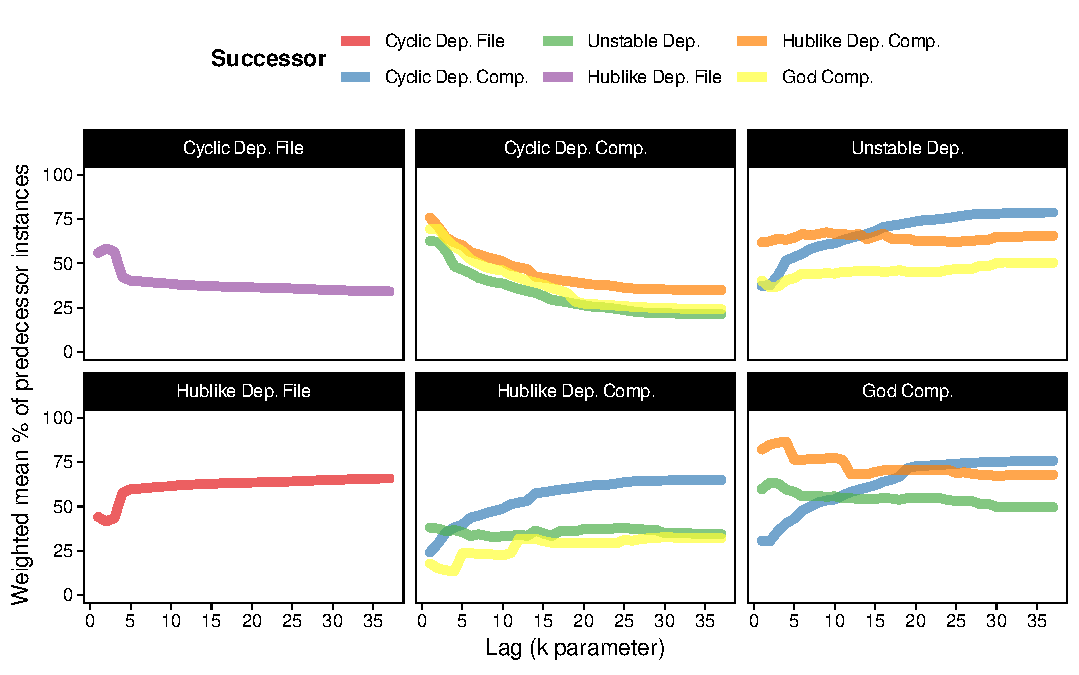
\includegraphics[width=0.95\textwidth]{c4/Fig11}
    \caption{The percentage of instances for each smell type that precede the other smell types, measured for different values of $k$. Each quadrant represent the predecessor smell type. Percentages are weighted by number of occurrences in each project for a given value of $k$.}\label{c4:fig:precedence}
\end{figure}

\section{RQ4 and RQ5 -- Practitioners and Architectural Smells}\label{c4:sec:rq-4-and-5}
\subsection{Data analysis methodology}\label{c4:sec:methodology-rq-4-and-5}
The qualitative analysis adopted the Constant Comparative Method (CCM) \cite{Glaser2017, Boeije2002}, part of Grounded Theory \cite{Glaser1968}, to deduct valuable insights from the interviews. Grounded Theory (GT) is one of the most important methods in the field of qualitative data analysis. It has been used extensively within both social sciences and software engineering and provides a structured approach to process and analyse the data collected from multiple sources. GT increases the theoretical sensitivity of the researcher as the data analysis progresses and eventually allows to formulate hypotheses and theory \cite{Glaser1968}.

As mentioned above, we have used CCM, an inductive data coding and categorization process that allows a unit of data (e.g., interview transcript, observation, document) to be analyzed and broken into codes based on emerging themes and concepts; these are then organized into categories that reflect an analytic understanding of the coded entities \cite{Mathison2005}.

The qualitative data analysis process is presented in Figure \ref{c4:fig:qualitative-analysis}. During the first phase (Phase A), the collected material (i.e. interview recordings) was studied and a code map was created to organise the codes used to tag the data.
After completing this phase, the coding process started (Phase B), which also involved updating and re-organising the codes based on the new understanding of the data.
As new interviews were recorded, transcribed, and coded, the data was also gradually analysed and notes were taken with the aid of the codes in the data (Phase C).
To aid with the organisation of the codes, we created a network of codes\footnote{See replication package.}, where each code was linked to other codes based on their relationship.
In total, two rounds of coding where done, the first one as interviews were transcribed, and the second one after the transcribing process was completed, to ensure that the codes added along the way were present in all the data.
Additionally, coded quotations from the interviews that referred to the same topic (e.g. two participants referring to the same event) were linked together to help navigate the quotations during data analysis. This process included both intra- and inter-document quotations, where documents refer to interview transcripts.
The whole process was performed by the first author of the chapter, while the second author reviewed the codes and coding schemes as they were developed to reduce the risk of biases (e.g. confirmation and information bias).
To automate the data analysis as much as possible, we relied on Atlas.ti \footnote{See \url{https://atlasti.com/}.}, a dedicated qualitative data analysis tool.

\begin{figure}
    \centering
    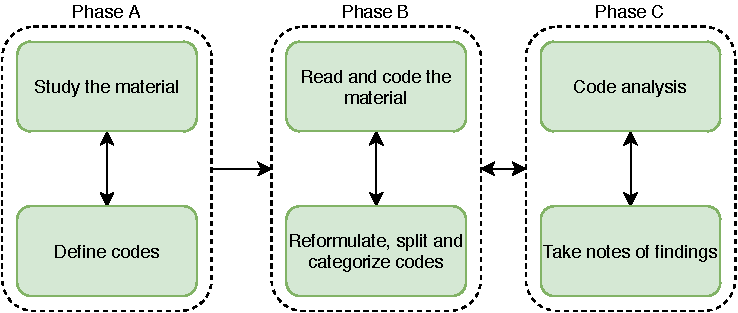
\includegraphics[width=.8\linewidth]{c4/Fig12}
    \caption{The phases of the qualitative data analysis process.}\label{c4:fig:qualitative-analysis}
\end{figure}

\subsection{Results}\label{c4:sec:results-rq-4-and-5}

\subsubsection{RQ4 -- Support to practitioners}\label{c4:sec:results-rq-4}
\paragraph{Overall considerations}
Most of the interviewed participants stated that the reported results resembled what their intuition and expectations were prior to seeing the report.
\begin{quote}
    \emph{``It was more like a confirmation, because yeah, since I was busy with this project for five years, I had a feeling where the “bottlenecks” were and which components were changed the most."}
\end{quote}
Many practitioners also reported that the results correlate with the parts of the system they experienced issues (either currently or in the past).
The most unexpected result for some participants was the number of Cyclic Dependencies affecting the files within a certain component; they mostly underestimated it, particularly for components that are relatively new.
\begin{quote}
   \emph{``Something that I didn’t knew is that Component X and Component Y are also not doing good while they are relatively new components. "}
\end{quote}

This begs the question whether the architectural smells analysis actually helps architects and developers, since they already know where the issues are. Participants mentioned that the report provides them with the following benefits: \emph{(a)} a ``good view" of \textbf{where cyclic dependencies are} so they do not have to ``grope in the dark", \emph{(b)} a way to \textbf{prioritise} the future improvements based on where exactly the current smells are, \emph{(c)} a good idea of \textbf{how complex and extended a specific change} (e.g. add/modify a requirement) could be, \emph{(d)} a way to \textbf{track the issues}, making them visible to the rest of the team, \emph{(e)} a clear approach to determine \textbf{when an issue has been fixed}, and \emph{(f)} a way to find out if the \textbf{problem reappears} in the future.

A common point among all these benefits is that they all contribute, in one way or another, to sharing the knowledge of the problems present in the project with all team members in a way that would otherwise be tacit.
One participant also highlighted the usefulness of the information provided for new team members:
\begin{quote}
    \emph{``[...] this will be very useful, for example, to any person coming to the team or a new architect of a team. Graphs like this will then provide years of experience in one go."}
\end{quote}

Transferring and tracking knowledge as a team can be rather cumbersome \cite{Rus2002}, so automating this task with a tool, is an added value that several practitioners appreciated, and expressed a desire to integrate into their workflow in order to receive periodical reports.

Finally, the fact that the reported issues are already known to practitioners, is considered as a positive outcome of our study. It indicates that the AS we were able to identify are true hotspots within the system (though quantifying this using the Precision and Recall metrics was out of the scope of this study).
It is also worth noting that in some cases, the problematic components highlighted in the results were already part of the quality improvement roadmap that one designer proposed to the architect responsible for their project. 

\paragraph{Specific feedback}
After having established that the analysis actually provides an added value to the practitioners, we now describe which details provided them with the most insights.

In terms of the information contained in the report that the participants marked as useful, or referenced while explaining something, or implied that it allowed them to plan future activities accordingly, we have the following:
\begin{itemize}
    \item the dependency graph of components, as it provided an overview of the current state of the system's architecture;
    \item the heatmap showing what components were affected by most smells (and what type these smells were), as it allowed to identify the hotspots of the systems quickly, and plan accordingly;
    \item the total number of smells (divided by type) over time, as it showed the trend of the quality of the system;
    \item the histogram with the number of incoming and outgoing dependencies for each component in the current version, as it shows an overview of the system like the dependency graph but allows for an easier comparison between the components;
    \item the number of components involved in a smell (i.e. the Size characteristic), and other characteristics (like shape of a cycle), as it provided a quick summary about the smell and its possible effect on the system in a glance;
\end{itemize}
The fact that all this information could be generated automatically, with very little configuration by the user, and on-demand, was greatly valued.

\paragraph{Missing information}
The participants also provided their opinion on what information is missing from the report.
A common feedback that we received is the lack of ability to dive into the details of a specific smell, and visualise the relationship between the affected components, how they interact with their neighbours, and other contextual information useful to fix that smell.
However, it is fair to note that this was also not the purpose of the report to begin with; rather, it was designed to provide a general overview of the architectural smells present in the system.


\subsubsection{RQ5 -- Impact on Maintainability and Evolvability}\label{c4:sec:results-rq5}
During the interviews, practitioners shared several experiences concerning the maintainability and evolvability of components that were affected by smells.
Although the majority of these anecdotes referred to different events and projects, most of them had enough similarities to allow us to identify a few patterns in the types of issues faced when trying to maintain or evolve the system.


\paragraph{Ripple effects}
The most common type of problem is related to the \emph{ripple effects} of changes. Making any kind of change to components affected by smells, is a 
troublesome process that required additional effort to carry out.
This additional effort was mostly due to changes that would \emph{propagate} to parts of the system that were partially, or totally, unrelated to the original change.
\begin{quote}
    \emph{``When I consider our changes in the past, these components are almost always touched. Depending on whether we can keep a change internal to a component or not, it may be that the change propagates to interface of this component. If it does, then we get this domino effect.''}
\end{quote}
Change propagation (or change ripple effects) is problematic, as changing a component might propagate to different components belonging to different teams.
This often means that a simple change could impact multiple teams, thus requiring further synchronisation between the teams to get it done; ultimately, the change becomes much costlier.
The same participant that gave the previous quote, provided an example of this phenomenon after being asked whether he/she noticed a correlation between changes and the components affected by smells:
\begin{quote}
    \emph{``Two years ago I made some changes in Component X that propagated to 56 components only because we changed the interface of that component. The changes we made were big and not backwards compatible and we had to change almost 60 different components in 5-6 teams, and it took a year to get everything done.''}
\end{quote}
In this case, Component X was affected by both God Component and Unstable Dependency, and the subject also mentioned Unstable Dependency as the most critical type of smell before providing this example.
We cannot claim of course, that the presence of the two smells are directly the cause of the ripple effects of these changes in other components.
However, the answers provided by the subjects directly link the presence of smells with an increased change propagation and change-proneness in the affected and neighbouring components.

On a similar note, another practitioner mentioned an example where changes in the code belonging to low-layer components that control the hardware, propagated to components in higher layers, even though that was not supposed to happen.
The low-level components were responsible for controlling some underlying sensors and hardware with the goal to support the hardware of a new machine.
The changes to these components triggered changes that rippled upward in the hierarchy of layers and the amount of work required to complete the update process was \textbf{initially underestimated}. The subject linked this particular case to both Hublike Dependency and Unstable Dependency: the low-level hardware components were controlled by a middle-level component, which was both unstable and a hub, and the high-level components depended on it.

Finally, ripple effects were also commonly associated with god components and their inherent internal complexity as well as with the fact that they usually contained a lot of legacy code. Making changes to complex god components was considered a \emph{risk}, because every change could affect multiple files and change the behaviour in unknown parts of the system or component (as pointed out by one of the practitioners this is also due to the inadequacy of their tests to test for regression).
Some god components contained files that were so tangled (i.e. affected by cycles) that even a simple change would have impacted several other files.
 

\paragraph{Architecture Erosion}
In addition to changes rippling to external components, participants also provided examples that the presence of smells is a sign of \emph{architectural erosion} \cite{Perry1992}: the gap between the original, intended architecture and the actually implemented architecture, that happens due to the continuous maintenance and evolution activities.

One of the interviewed architects explains their struggle with implementing the parallelisation of two tasks in order to speed up the production throughput of the whole machine. 
The tasks were both implemented by a certain Component Y, which, over time, became so complex and intricate (and also contained legacy code) that made it too difficult to proceed with the implementation of the desired feature (i.e. parallelisation) before actually refactoring the code\footnote{Note that the refactored version of the code was implemented in another component, which, when it is ready, it will supersede Component Y.}.
\begin{quote}
    \emph{``In your results Component Y is both a god component and a hublike dependency. [...] We do have maintenance issues in that component, so we want to split it to smaller functions because it has a lot of functionality and is quite a drawback to scale the functionality [...]. The road map that we had for improving it is to split the component to allow us to do the two things in parallel.
    To make that first step it was very painful in the short term, but once we got the hang of it it’s been improving a little bit.''}
\end{quote}
This example reflects how an important evolution of the system that would provide a tangible improvement for the customer, is hindered by: a) the centralisation of functionality in a single component (i.e. the two tasks), which is typical of hubs; and b) the aggregation of implementation (and legacy code), which is typical of god components. This component was originally not meant to be so large and complex, but erosion happened over time.

Cyclic dependencies among components were also mentioned by multiple architects as a sign of architecture erosion.
One architect mentioned an interesting example of how cycles were creating, over time, various problems that confused the team about what responsibilities were implemented by what component.
\begin{quote}
    \emph{``We also had a famous cyclic dependency between Components Z, U, and V, which had all kind of interesting things. Over time, sometime one controlled the other and sometimes the other controlled the first. That always gave us problems. So we are now actively redesigning that part to get rid of that cycle.''}
\end{quote}
This is a textbook example of the detrimental effects of cyclic dependencies among components on the maintainability of the system. Since the original architecture is eroded, developers first have to reverse engineer the responsibilities of the components at that point in time before applying the desired change to the system.

Moreover, another architect provided a very interesting anecdote about trying to refactor one cyclic dependency, showing how hidden dependencies, and the resulting complexity can ultimately have a direct impact on the company's business.
\begin{quote}
    \emph{``Last year we tried to remove a cyclic dependency by introducing a pattern to remove part of the cycle. However, we were not aware of all the legacy functionality within that component, and while removing the cycle, we missed some of the dependencies. This led to a lot of escalation in the field and we had to fly over to our customer to explain why this happened. It was actually a combination of god component and cyclic dependency. It was a real pain and the whole team had to work for two or three months to get it solved.''}
\end{quote}

In conclusion, all the examples mentioned in this section highlight how certain smell types (i.e. god components, hubs, and cycles), in one way or another, hinder the evolution -- and even the refactoring -- of the system and reflect its architecture erosion, further preventing developers to deliver new functionality to the customer.

\paragraph{Bugs and errors}
Practitioners also shared stories on how certain smell types affect the correct functioning of the system.

Cyclic dependencies, for instance, were mentioned several times (by multiple subjects) as a type of smell that causes errors at runtime, such as deadlocks, synchronisation issues of two or more tasks working together, or reduced throughput.
\begin{quote}
    \emph{``For example, if we look at the cyclic dependencies in the report. And look at the first one you see, this is basically the interaction between dose control peripherals. Those [components] are basically sensors, and these peripherals should only talk to [a master component] without talking between each other. […] when you have time-critical data coming in, this can lead to some timing errors in the field and sometimes deadlock.''}
\end{quote}

God components were also mentioned when discussing bugs and errors, though cycles among components were more dreaded because they had a direct impact on the observed behaviour of the system by the customer.


\paragraph{Communication}
Finally, practitioners also reported communication-related issues during maintenance and evolution that they associated with the presence of smells.

In this company, every component has a component owner, who is responsible of tracking changes, reviewing changes, handling questions from other owners or developers, as well as other organisational tasks.
This causes owners of components that are essentially god components to be overwhelmed with requests because their components implement a lot of functionality, have a lot of responsibilities and a lot of other components depend on them. 

Another problem in this category are code reviews of smelly components that contain a lot of files that change.
When the designers and architects meet to discuss and approve the changes in the code reviews, several discussions and arguments arise about the impact of each change, how to interpret the changes, and even what customers might be affected by certain changes thus creating confusion and ultimately delaying the development process.


\section{Discussion}\label{c4:sec:discussion}
In this section we discuss the results obtained in this study and compare them to related work. Each subsection focuses on a significant aspect of the results we obtained from each research question. 

\subsection{Entanglement of dependencies}
An interesting observation stemming from the results obtained from RQ1 is that most of the cycles at file-level pose (in themselves) little threat to the maintainability level of the system as they (a) were not associated with bugs by our practitioners (unless they crossed the component border) and (b) only half of them survive for more than a year.
However, we noticed that when multiple cycles co-exist within the same component they create an  \textbf{entanglement of dependencies} that ultimately affects the clarity, testability, reusability, and the ability to anticipate the effects of changes of the parts affected by the cycles.
In fact, Lippert \cite{Lippert2006} hinted (back in 2006) at the possibility that cycles among files (or classes) may affect those aspects of Maintainability; the results presented in this chapter corroborate his heuristics with empirical evidence.
Our results also align with those of Mo et al. that supported such heuristics in their industrial study \cite{Mo2018}.
More specifically, they found that clique-shaped cycles among files generated a considerable amount of maintenance activities in the affected components. 
The high coupling created by the presence of several cycles among the same group of files (such as cliques, or quasi-cliques) increases the \textbf{maintenance effort} required to maintain them.

On a similar note, Lippert had also mentioned that, while spaghetti code (i.e. \emph{goto} statements) is thought to be a thing of the past, modern software code still presents similar structures; but, instead of occurring at function or statement level, it involves files and components.
In other words, we \textbf{never really got rid of spaghetti code}'s negative effects (confusion, difficulty applying changes, intertwined logic etc.); we just solved the most explicit part of the problem, the one showing up in the code (i.e. the goto statements). 
Now we are facing the part of the problem that affects the way we organise code (files and components), where the negative effects can potentially have a larger impact.
The findings of this study show exactly this particular aspect, highlighting how practitioners struggle with maintaining entangled files and components and \textbf{need assistance} to manage the intricate structures that arise in their codebase.
Therefore, we advise researchers, to focus more on building tools and frameworks that reduce the burden of dealing with this particular type of issues, as well as on making these means more \emph{accessible and usable} by the industry.
While tools like \textsc{Arcan} are a first step towards this goal, the findings of this chapter can  guide research activities in this direction too.
One example stems from our results on the introduction order of architectural smells. A machine learning tool that precisely predicts the introduction of new architectural smells in a component could be of great value to practitioners.

\subsection{Persistence of smells}
The results of RQ1.2 show that 50\% of Cyclic Dependencies do not survive more than 10 versions after their appearance.
Bavota et al. \cite{Bavota2015} studied the relationship between refactorings and code smells, and, surprisingly, their findings show that only 7\% of code smells are removed because of \emph{intentional} and specific refactoring activities. 
Should this finding be valid for architectural smells too, it would mean that only a \textbf{small percentage of architectural smells are intentionally removed by applying refactorings}.
The remainder of architectural smells may be therefore removed as part of the development activities related to the evolution of the system.
In Chapter \ref{chap:2}, we also found that architectural smells' density over time is mostly constant in the long-term, meaning that as AS are removed from the system, they are also eventually replaced by others.
Cedrim et al.'s study \cite{Cedrim2017} report a similar percentage of code smells (i.e. 9.7\%) removed by refactorings, and, more interestingly, 33.3\% of refactorings actually resulted in the introduction of new code smells (most of which were never removed from the code).
Given our results, we could hypothesize that the same phenomenon may also occur for architectural smells: \emph{targeted refactorings potentially account for the minority of the architectural smells removed over time in a system}.
A possible explanation is that given the fact that architectural smells are not easy to visualise without proper tooling, then it is hard for developers and architects to realize what problem they are facing and thus act accordingly.

\subsection{Comparison with Java OSS}
Comparing the results obtained in RQ1 of this study with the results obtained in our previous study on Java OSS from Chapter \ref{chap:2}, we note both similarities and differences.

\paragraph{Evolution of smells}
In both cases, we found that the size of the smells either stays constant in size or increases over time while the smell density of the system remains constant.
Specifically, the size of the analysed systems (both C/C++ and Java) grows over time which entails that AS grow both in number and in size over time; this holds for both industrial C/C++ and Java OSS.
This is an expected result because software systems are expected to: (1) continue to grow over time (more lines of code are added every day); and (2) increase in complexity over time (more smells are added every day and existing smells may increase in size) \cite{Lehman1980}.

One difference we observed was that for OSS projects, UD had a dominant decreasing trend for its PageRank characteristic as in Chapter \ref{chap:2}; this was not the case for C/C++ systems.
It is hard to objectively interpret this disparity given the different programming languages. However, we conjecture that the open source community is more successful in driving the more unstable components away from the centre of the system, where the maximally stable, core abstract components should reside \cite{Martin2018} and away from the implementation provided by the external ones.
It is important to note that the majority of Java OSS projects present in our previous study from Chapter \ref{chap:2} were Apache projects, which are known to follow high software quality standards.

\paragraph{Survivability of smells}
We noticed several similarities between Java OSS and the industrial C/C++ projects we analysed.
Both exhibit a trend where UD smells are the most persistent type of smell across the projects analysed.
HL smells follow UD in second place, which in turn are followed by CD smells (GC smells were not included in our original study).
Additionally, HL smells among components are more persistent than HL smells among files and cycles among components were less persistent than cycles among files in both types of systems.
Given these similarities, we can conclude that different architectural smell types exhibit the same pattern of persistence regardless of the type of system they are detected in.

However, we also noticed one important difference between the smells detected in Java OSS and C/C++ industrial systems: all \emph{smell types exhibit longer lifespans in the industrial systems}. 
This aligns with the feedback collected from our interviews with ASML engineers (see Section \ref{c4:sec:results-rq-4-and-5}): making changes is hard, they require a lot of coordination between teams, certifications, code reviews, and a lot of effort in general.
The way ASML defines dependencies among components may also have had an impact on the survivability of smells. ASML components use a custom mechanism to expose their interface to other components. Thus, if a component communicates with another component through that interface, it is very likely that the dependency between those two components is there by design and not accidental or involuntary. This implies that it is less likely for that dependency to be removed in the future, and thus all smells relying on that dependency (e.g. like a cycle) will keep existing.
Ultimately, this custom mechanism, and the rigorous engineering processes between and within teams translate into an increased amount of time necessary to make a complete change to the system, which is also reflected in our data.

Finally, cycle shapes also exhibit the same patterns identified for Java OSS systems.
We especially observed that tiny cycles are outliving all other shapes in both types of systems, showing how this shape is very likely to be intentional and/or less harmful than the other types of cycle shape.

\subsection{Overlaps}
The results obtained from RQ2 show that, except for a few outliers, all smell types are \emph{likely} to overlap, \textbf{amplifying their impact on maintainability and evolvability} and \textbf{giving components more than one reason to change}, thus breaking the Single Responsibility Principle (SRP) \cite{Martin2018}. 

Our conversations with practitioners from RQ5 provide evidence to support this very claim, as they mentioned multiple examples where they associated two or more smells with the maintenance issues they were experiencing.
These results emphasise the importance of handling overlaps between architectural smells and, more importantly, preventing their introduction in the first place.

From our quantitative analysis emerged that cycles are pervasive in the system and they tend to appear as precursors to other smell instances, as they exhibit a high precedence rate (with $k = 1$).
This could mean that the presence of cycles in the system is likely to ease the introduction of other smells.
As a result, other smell types tend to have a high overlap rate (from 52\% to 77\% of instances, depending on the smell type) with cycles.
On the other hand, HL instances exhibit the opposite behaviour and have a low precedence rate but a rather high overlap with other smell instances (59\% to 77\% of HL instances).
This gives us an insight about the interplay between architectural smell instances of different types.
Cycles act as \emph{catalysts for more complex structures}, such as HL, to arise and negatively affect the maintenance of the affected components and files.
There were plenty of occasions where we observed star-shaped (see Figure \ref{c4:fig:cycle-shapes}) cycle instances of which central element was also affected by a HL instance.
Indeed, in our RQ3 results, one of the drawbacks of a Hublike Dependency smell is that it aggregates responsibilities that it either delegates or implements itself.
Which just by itself breaks the SRP principle and impacts negatively maintainability.
For UD instances, on the other hand, tightly coupled structures such as cycles have an inherently high instability \cite{Martin2018}, which in turn reflects to the component depending on them, thus creating an UD instance.
Understanding how and why CD instances are precursors to other smell instances is an interesting opportunity for future work.

\subsection{Feedback from practitioners}
From the results of RQ4, we found that AS analysis is quite useful to practitioners, especially for \emph{monitoring} purposes, rather than \emph{identification}: practitioners are mostly aware of the hotspots in their systems but they do need assistance in \emph{tracking} and \emph{quantifying} their presence deterministically.
Interestingly, these findings match what Mo et al. \cite{Mo2018} encountered but partially contrast the findings of Martini et al. \cite{Martini2018}, as in their case, practitioners were mostly unaware of the architectural smells in their system but found the information provided by smells still useful.

A possible explanation for this discrepancy is the fact that most of our participants have a long experience working for the company: they worked as developers for a long time in a project before becoming architects (or senior developers) of the same project. This means that they have a much more in-depth understanding of the problems in their system, so the information provided by a tool can mostly confirm this understanding.
We can only conclude that the level of awareness of developers of the smells in their system varies from subject to subject. In fact, a recent study on the topic \cite{Arcelli2020} showed that developers' awareness of smells ranges from 26\% of all the smells detected in the system up to 78\%, depending on the participant.
This has a clear implication for researchers: if they are able to show the same information that a senior developer (or architect) is already familiar with, to all members of the team, regardless of their experience, then architectural smell analysis does \textbf{provide an added value to the team}.

Another common finding with Mo et al.'s work \cite{Mo2018} is the feedback of practitioners concerning the created reports.
Similarly to our study, Mo et al. also prepared reports that summarized the results to the developers and architects of the system.
These were very much appreciated by the developers and engineers in the companies of the two studies, and as a result, both companies showed interest in creating an integration with their own CI/CD to automate the analyses and provide daily (or weekly) reports.

One finding that was not reported by the subjects interviewed by Mo et al. is that our practitioners also highlighted the usefulness of our reports to new team members, and how they allow an easy transfer of knowledge to the less experienced members.

\subsection{Applying changes to the codebase}
The results of RQ5 show that practitioners struggle to maintain the components affected by architectural smells in a sustainable way. The main reasons include change propagation and the effects of a change in unknown parts of the codebase, during both typical maintenance (i.e. bug fixing, adaptations to new technologies) and evolution (addition of new features) tasks.
Previous studies from the literature corroborate these findings with data extracted by mining software repositories. Le et al. \cite{Le2018} found evidence that in open source Java systems the presence of architectural smells correlates with change-prone artefacts. Similar findings were also reported by Oyetoyan et al. \cite{Oyetoyan2015} on circular dependencies specifically.

The study of Vaucher et al. \cite{Vaucher2009} looked at the change proneness of God Classes, and showed that some God Classes are significantly less change-prone because they exist by design. 
While their findings refer to a different type of artefact (i.e. a code smell that is similar to GC but not exactly the same), they offer an insight on why some of the subjects we interviewed dismissed God Components as less detrimental (than other GCs). Specifically, God Components that are made by design are more easily understood by practitioners, because they understand their design and are thus better able to handle their complexity. 

We can thus conclude that change-prone artefacts and architectural smells are \emph{highly correlated} as this relation has been identified both quantitatively and qualitatively as well as independently by different studies.
This \emph{strengthens} the evidence about the increased effort required to maintain artefacts affected by architectural smells and \emph{highlights} the importance for practitioners to manage architectural smells.

Mo et al. also report about the experiences of developers when dealing with ripple effects \cite{Mo2018}. For instance, Mo et al. report on how developers consider the risk of performing a change to a file and that sometimes this is underestimated. This is corroborated by our findings. However, we also provide extra information about the ramifications caused by changes both at a company level (impacting several other teams) but also about the shortcuts that developers take in order to avoid the risks imposed by those changes.
As an example for the latter case, some developers admitted to intentionally duplicating entire files in order to avoid impacting other files with their changes.
%for researchers to further investigate architectural smells management, similarly to what has been done for code-level issues such as code smells.

\section{Implications for practitioners}\label{c4:sec:implications}
Our results can help software engineers and architects to become aware of the side-effects associated with the presence of architectural smells within a large embedded systems company such as ASML.
Particularly, a few key points that practitioners should consider are the following:
\begin{itemize}
    \item the importance of \textbf{continuously monitoring} the presence of cycles among components/packages, as stated by the Acyclic Dependencies Principle \cite{Lippert2006}. Practitioners should especially oversee the components (or packages) that exhibit an excessive amount of internal cycles, as these may \emph{severely degrade} the overall maintainability of the component. On top of that, we also found that cycles are catalysts for other smells to arise;
    \item the \textbf{appearance of a Hublike Dependency} may be a clear signal that the affected part requires some refactorings, given that, as we found, this type of smell is likely to appear after other smells already affect a component.
    Cedrim et al. \cite{Cedrim2017} found that the most effective refactorings are the ones that target aggregator-like smells (such as Hublike Dependency and God Component), therefore this is a clear actionable point for practitioners;
    \item the \textbf{experiences shared by ASML} engineers can provide insightful details to other practitioners to avoid incurring similar issues such as change ripple effects, architecture erosion, and communication bottlenecks. To this end, practitioners should stick to architectural principles \cite{Martin2018} and guidelines and avoid the presence of severe architectural smell instances;
    \item the \textbf{integration of historical change-related information} of the components into decision-making processes through dashboards and reports. Our findings show that recurring changes are often associated with the presence of an architectural smell.
    Repairing artefacts that are commonly subject to maintenance work may ease the extra burden required to implement new features or fix bugs on the long-term.
\end{itemize}


\section{Threats to validity}\label{c4:sec:threats-to-validity}
We identified the potential threats to validity for this study and categorised them using the classification proposed by Runeson et al. \cite{Runeson2012}: \emph{construct validity}, \emph{external validity}, and \emph{reliability}.
Internal validity was not considered as we did not examine causal relations \cite{Runeson2012}.

\paragraph{Construct validity}
This aspect of validity reflects to what extent this study measures what it is claiming to be measuring \cite{Runeson2012}.
To ensure we measure how AS evolve and how practitioners experience AS, we developed a case study using a well-known protocol template \cite{Brereton2008} that was reviewed by the first two authors and an external researcher in several iterations to ensure that the data to be collected would indeed be relevant to the research questions.

A possible threat to construct validity is the correctness of the parsing algorithm for the proprietary parts of the C/C++ compiler adopted by the company of this study. 
To mitigate this threat, we manually validated the parsing algorithm with a list of well-known files and components that had dependencies defined by proprietary constructs in the code.
The whole process was also supervised by one of the architects taking part in the study.

Another threat concerns the detection of the smells considered in this project, which depend on the implementation offered by \textsc{Arcan}.
Lefever et al. \cite{Lefever2021} have shown that different tools for technical debt measurement (including DV8, CAST, and SonarQube, but \emph{not} \textsc{Arcan}) have divergent, if not conflicting, results regarding which files are problematic in a system.
This is due to the fact that different tools make different assumptions, use different definitions of a smell, and have different implementations of how to detect a smell \cite{Lefever2021}.
Therefore, we can only state that our quantitative results obtained through \textsc{Arcan} may not be fully comparable with the results obtained by other tools.
However, this would be the case \emph{even if we used any other tool}, as shown by Lefever et al. \cite{Lefever2021}. 
Having said that, this threat can be considered \emph{partially mitigated}, as the definitions of each architectural smell used by \textsc{Arcan} are based on independent, previous work.
In particular, CD is based on the Acyclic Dependencies Principles \cite{Martin2018,Lippert2006}, HL and UD on the definitions provided by \cite{Samarthyam2016,Martin2018}, and GC on Lippert's definition \cite{Lippert2006} (further improved upon by the authors of \textsc{Arcan}).
This cannot be said for other tools available, as many of them are based on previous work of the very authors of the tools, and therefore may potentially be biased.
Moreover, to guarantee that the results obtained by the \textsc{Arcan} tool are indeed in line with the definitions provided by previous work, the tool was used and evaluated in a number of studies \cite{Arcelli2016,Biaggi2018,Sas2019}.

Yet another threat concerns the methodology we used to select the subjects for the interviews. Instead of using a probabilistic approach (i.e. random sampling) to sample our subjects, we sampled them based on convenience and circumstance. 
This was mainly due to two factors. First, it was up to the architects of each team to approve the interviews with their engineers.
Second, we could not interview subjects from all of the projects we analysed, as not all project architects were willing to provide participants.
Nonetheless, we managed to interview a good number of subjects, with more than one person per project in almost all cases, different levels of seniority and a balance in roles. Therefore, we consider this threat as, at least partially, mitigated.

\paragraph{External validity}
This aspect of validity reflects to what extent the results obtained by this study are generalisable to similar contexts.

External validity is limited by the fact that we only analysed the projects belonging to a single company with its primary business focused on a single domain.
The threat is partially mitigated by the fact that our quantitative results corroborate previous findings from open source systems: even though we only studied architectural smells in one, specific context, the findings have good chances to be applicable to other contexts as well.
Our qualitative results, on the other hand, can be applicable to large companies that employ a similar development process such as the company subject of this study.

Another threat to the generalisation of our results is the fact that the studied projects are part of a software product line composed of several products (machines).
This poses the risk of limiting the applicability of our results to the specific context of companies that develop software product lines.
The risk arises because architects and engineers must take into account the reuse of their code in different products with different hardware configurations, which may not be the case for many other companies.
To mitigate this risk, we focused our attention on issues that can occur independently of the practices adopted to develop and manage the software assets of the company.
For instance, during our interviews, we obtained a few data points mentioning reusability-specific issues encountered by engineers, however, we opted to only include in our results those that are potentially applicable to other contexts in order to not limit external validity.

\paragraph{Reliability}
Reliability is the aspect of validity focusing on the degree to which the data collection and analysis depend on the researchers performing them.

While we cannot share our dataset for confidentiality reasons, we do, however, provide a replication package\footnote{Visit \url{https://doi.org/10.6084/m9.figshare.16884739.v1}.} containing a complete version of the study design of this study and a sample of the report we sent to our practitioners to allow researchers to reuse similar data visualisations in their future work.
Moreover, the tools used in this study are freely available online\footnote{\label{fn:tools}See \url{https://github.com/darius-sas/astracker} and \url{https://gitlab.com/essere.lab.public/arcan}.} to allow other researchers to assess the rigour of the study or replicate the results using a different set of projects.

Another threat to reliability is the bias towards the data introduced by the researcher performing the coding.
This threat was mitigated by having a second researcher inspect both the codes and the coding maps extracted during each round of coding. All the feedback received was then integrated and the subsequent coding sessions adopted the updated codes.
The analysis was also performed using well-established techniques already used in previous work on the same topic as well as also in different fields (e.g. survival analysis, in the biomedical sciences field).
Therefore, we consider this threat mitigated.

\section{Conclusion}\label{c4:sec:conclusion-fw}
In this chapter, we presented the results of an empirical embedded multiple-case case study performed using both quantitative and qualitative data. 
The data was collected by statically analysing 280 releases (spanning almost 3 years) across 9 industrial projects and by interviewing 12 subjects responsible for developing and architecting the projects under consideration.

To collect the quantitative data, we used a tool called \textsc{Arcan} to mine architectural smells (and their characteristics) from the over 20 millions lines of code available to us.
We then used different techniques to study the evolution of the architectural smells and understand how they evolve over time, how long they persist within the system depending on their type, and how they overlap with each other.
The findings show that smells grow over time in size, and that most of the detected instances do not persist for more than 2-3 releases. 
Moreover, most smell types were found to have high percentages of overlap with other smell types, meaning that it is not uncommon for components to be susceptible to problems caused by multiple types of smells, as also highlighted by our subjects during the interviews.

Indeed, practitioners found that our results aligned with their intuitions of where the issues were located and commented that tooling that helps them manage AS could be quite useful to them.
During the interviews, practitioners also mentioned rather interesting experiences where they struggled maintaining components affected by architectural smells, thus providing evidence of the negative effects of AS on Maintainability.

In conclusion, this chapter provides a much clearer, and backed by empirical evidence, view on the issues experienced by practitioners in the presence of AS.
One aspect that was of particular concern for many practitioners was the change ripple effect that was associated with the presence architectural smells.
In the upcoming chapter, we designed a case study to investigate the relation between architectural smells and source code changes from several points of view using statistical analysis.


\section*{Acknowledgements}
We would like to thank the Center for Information Technology of the University of Groningen for their support and for providing access to the Peregrine high performance computing cluster.

Lastly, many thanks to ASML for agreeing to give us access to their codebase, allow to run our analyses, and interview their engineers.

\section*{Declarations}
\subsection*{Availability of data, material, and code}
The data collected in this chapter is not available publicly as it belongs to ASML.
We do however provide a replication package at the following link \url{https://doi.org/10.6084/m9.figshare.16884739.v1} that contains the protocol we used to collect the data and an anonymised report that we showed practitioners.
The package also includes the R code we used for data analysis.
The two tools we used to carry out the analysis are also available online (see footnote \ref{fn:tools}), though they do not contain the modifications applied to support ASML's code.

\subsection*{Consent to participate}
All subjects of our interviews were asked whether they would agree taking part in the interview beforehand. Interviewees were also informed of the possibility that excerpts from the interviews may be used in a published version of the manuscript.


% % Paper 4 - 
\setlength{\headheight}{1.2cm}
\renewcommand{\publ}{\flushleft\footnotesize{Based on:\\[0.1cm]
		\textit{``On the relation between architectural smells and source code changes''} \\[0.1cm]
}}

\chapter{On the relation between architectural smells and source code changes}
\label{chap:5}


\begin{Abstract}
	While architectural smells are one of the most studied type of Architectural Technical Debt, their impact on maintenance effort has not been thoroughly investigated.
	Studying this impact would help to understand how much technical debt interest is being paid due to the existence of architecture smells and how this interest can be calculated.
	
	This work is a first attempt to address this issue by investigating the relation between architecture smells and source code changes. Specifically we study whether the \emph{frequency} and \emph{size} of changes are correlated with the presence of a selected set of architectural smells.
	We detect architectural smells using the Arcan tool, which detects architectural smells by building a dependency graph of the system analysed and then looking for the typical structures of the architectural smells.
	
	The findings, based on a case study of thirty-one open source Java systems, show that $87$\% of the analysed commits present more changes in artefacts with at least one smell and the likelihood of changing increases with the number of smells.
	Moreover, there is also evidence to confirm that change frequency increases after the introduction of a smell and that the size of changes is also larger in smelly artefacts.
	These findings hold true especially in medium-large and large artefacts.
\end{Abstract}

\section{Introduction}
Architectural smells (AS) are defined as \emph{``commonly-used (although not always intentional) architectural decisions that negatively impact system quality''} \cite{Garcia2009}.
AS manifest themselves in the system as undesired dependencies, unbalanced distribution of responsibilities, excessive coupling between components as well as in many other forms that break one or more software design principles and good practices, ultimately affecting maintainability and evolvability \cite{Lippert2006}.
We note that the presence of AS does not always inevitably indicate that there is a problem, but it points to places in the system’s architecture that should be further analysed \cite{Lippert2006}.
Architectural smells are considered as a type of architectural technical debt (ATD), as they (may) result in increased complexity and \emph{``can make future changes more costly or impossible''} \cite{Avgeriou2016}.
The interest of the research community in AS has grown exponentially over the past years: according to a systematic mapping study by Verdecchia et al. \cite{Verdecchia2018}, they are one of the most studied types of architectural technical debt.

Research work on AS has ranged from broad studies that define new smell types and study their evolution over time \cite{Arcelli2016,Oyetoyan2015,Le2015}, to more specific ones that focus on a particular architecture style (e.g. AS in systems built with Model-View-Controller, or Microservices \cite{Neri2019}).
Few studies, however, have extensively investigated the impact of AS on maintenance effort. While AS are considered detrimental to software maintenance, forcing developers to pay high technical debt interest \cite{Garcia2009}, there is little empirical evidence to explore and confirm this phenomenon.
Although there has been research on the impact of code smells on maintenance effort, architectural smells seem completely independent from code smells \cite{Arcelli2019}, and arguably more severe. 

This study addresses this gap by exploring the impact of a specific set of AS on maintenance effort in terms of the actual changes made by developers to the source code.
Specifically, we compare the  \emph{frequency} and \emph{size} of changes between source code artefacts affected and not affected by architectural smells. We perform the comparison both by controlling for the size of the artefacts and without any control for size, to eliminate size as a confounding factor.
We consider \emph{change frequency}, i.e. the number of times an artefact was changed across multiple versions, and \emph{change size}, i.e. the number of lines of code added, deleted, and modified\footnote{See Section \ref{c5:sec:data-collection} for a full description.}, as proxies of the effort spent, based on previous work: change frequency is a factor that was found to affect maintenance effort \cite{Sjoberg2013,Olbrich2009}, whereas change size (also referred to as code churn, or Total Amount of Changes - see Section \ref{c5:sec:data-collection}) was used to estimate the effort in previous studies \cite{ElEmam2000,Mockus2000}.
This can give an \emph{indication} of how much technical debt interest (rather than the actual interest per se) is paid by developers due to the presence of the detected smells (not all changes entail paying interest - see Threats to Validity section).
Furthermore, our findings can be used towards building a model to calculate, based on actual changes, the ATD interest \cite{Avgeriou2016} paid when maintaining artefacts affected by AS.

The architectural smells considered in this study are Cyclic Dependency (CD), Hub-Like Dependency (HL), Unstable Dependency (UD), and God Component (GC) \cite{Arcelli2016, Lippert2006,Sas2019}.
We selected to study these smells as they are some of the most prominent architecture smells, and there already exist tools that provide their automatic detection.

The novel contributions of this study are: (1) the vast majority of related work examines code smells, while we focus on architectural smells, which were found to be independent from code smells \cite{Arcelli2019}; (2) we study 4 different types of AS, and only CD were previously investigated by other studies, whereas the other three were overlooked; (3) we provide a new, interesting view of how AS affect artefacts before and after the introduction (RQ2).

The rest of the paper is structured as follows:
Section \ref{c5:sec:related-work} summarises similar work from the literature; Section \ref{c5:sec:design} describes in detail the goals, research questions and the selected projects of this study; Section \ref{c5:sec:data-collection} reports the data collected as well as the collection process; Section \ref{c5:sec:data-analysis} presents the data analysis procedures; Section \ref{c5:sec:results} reports and examines the obtained results; Section \ref{c5:sec:discussion} discusses our interpretation of the results and compares them with similar findings from the literature; Section \ref{c5:sec:limitations} enunciates the threats to the validity of this study; and finally, Section \ref{c5:sec:conclusion} concludes the paper and considers possible future work.

\section{Related work}\label{c5:sec:related-work}
\subsection{Impact of Architectural Smells}
In a recent work, Le et al. \cite{Le2018} defined a set of six architectural smells based on an automated reverse architecture model extraction. Next, they investigated whether files affected by architectural smells (i.e. smelly files) are more likely to have issues (extracted from issue-tracking systems) associated to them than clean files.
Additionally, they also checked if smelly files are more change-prone than clean files.
The case study was performed on eight different open source Java systems and the results confirmed that smelly files are more fault- and change-prone in the eight systems analysed. 
Contrary to the work of Le et al. \cite{Le2018}, in our work we investigate a different set of architectural smells based on concrete software artefacts, rather than on architectural recovery views; we use thirty-one projects, rather than eight; and we measure several facets of change-proneness (not only the number of commits a file has changed), using a well-established suite of metrics. 

Oyetoyan et al. \cite{Oyetoyan2015} have studied the relation between Cyclic Dependency (CD) and the change frequency of the affected classes near them on twelve Java open source systems.
They investigated both general CD between classes and special kinds of CD (e.g. cycles that contain both parents and children classes, abbreviated as STK, and cycles across branches of the package containment tree) that have been conjectured to be particularly undesirable.
Their results show that the presence of cycles does increase the change frequency of the classes affected and of the neighbour classes, but this is not true for classes affected by STK cycles in most of the systems considered.
Moreover, their findings also suggest that classes belonging to cycles spanning across branches of the package containment tree (the tree of the packages) do not exhibit a higher correlation with change frequency.
Our work differs from this study in the following aspects: we investigate four types of smells, including CD, both at class and package level; our data includes more systems and more commits per system; and we use multiple well-established metrics to measure change.

\subsection{Impact of Anti-patterns, Design Patterns, and Design Smells}
Khom et al.  \cite{Khomh2012} investigated the effect of antipatterns (classes that embody poor design choices and stem in-between design and implementation \cite{Khomh2012}),  on class and change proneness. More specifically, the authors investigated whether classes participating in antipatterns have a higher likelihood than others to change or be involved in issues documenting faults.
Their study focused on four open source Java systems and a total of fifty-four releases. Their findings confirmed that classes participating in antipatterns are more change prone than others. Specifically, the \emph{MessageChain} antipattern has been found to consistently have the greatest impact on change proneness across all the four systems analysed. The impact of the other antipatterns largely depends on the studied system.
Concerning fault proneness, the results are very similar to what was observed for change proneness.

Another work on antipatterns and their relation with changes and faults was published by Jaafar et al. \cite{Jaafar2016}.
In their work, rather than focusing on problematic classes as previous studies, they focused on classes that depend upon classes affected by antipatterns and/or participate in design patterns.
Their work focused on six design patterns and ten antipatterns detected throughout thirty-nine releases of four systems.
The findings indicate that classes having dependencies with antipatterns are more prone to fault, while this is not always true for classes with dependencies with design patterns.
Additionally, the findings also show that classes depending upon antipatterns are more prone to logic faults and structural changes, whereas classes depending on design patterns are more prone to code addition and syntax faults.

Sharma et al. \cite{Sharma2020} conducted an empirical study to investigate the relationship between design and AS in C\# projects, where what they call design/architectural smells correspond to our distinction class/package smells. They studied correlation to check whether, given pairs of design and architectural smells which capture the same concept at different granularities, one of the two is superfluous. They studied collocation and
% trying to understand if certain types of design smells may act as indicators for specific AS; 
causation, by investigating temporal relationship between design and AS to figure out whether some types of smells cause the others. Thanks to their analysis, they found evidence of the individuality and uniqueness of design respect to AS.


\subsection{Impact of Code Smells}
Aniche et al. \cite{Aniche2018} have studied the impact of code smells on change and fault-proneness in Model-View-Controller (MVC) architectures prior to performing a qualitative analysis involving the developers of the 120 projects they considered.
The projects were automatically extracted from GitHub, and the authors defined a set of smells specifically tailored for the MVC architecture by surveying 53 developers.
The results concerning change and fault proneness show that classes affected by smells are more prone to change than non-smelly classes; traditional smells seem to have a stronger negative impact, although when controlling for size the difference is less marked on change proneness.
No impact was observed on fault proneness when controlling for size for both MVC-specific and traditional smells.

Another study on code smells and change-proneness was done by Khomh et al. \cite{Khomh2009}. In their work, the authors study the impact of 29 code smells on change proneness in 2 open source Java projects.
More precisely, they investigate whether smelly classes are more change-prone, how the number of smells influences this aspect, and differences in this impact between the different smell types.
Their findings show that smelly classes are in fact more change prone in both projects analysed. Additionally, they also show that a higher number of smells often implies a high change proneness. They also found that \emph{HasChildren}, \emph{MessageChainClass}, \emph{NotAbstract}, and \emph{NotComplex} smell types have the highest change proneness, but this is heavily project-dependant.

This study, in contrast, focuses on architectural smells, and as it was found in a previous study, architectural smells are independent from code smells \cite{Arcelli2019}.
Moreover, architectural smells, contrary to code smells, affect multiple classes and/or packages, have complex structures (e.g. dependencies among the affected components), and require large refactorings in order to be removed \cite{Lippert2006}.
This means that research on code smells is not applicable to architectural smells, and the only similarity with code smells in this regard is that each type of architectural smell needs to be investigated individually.


\section{Case study design}\label{c5:sec:design}
The present study is designed and reported following the guidelines published by Runeson et al. \cite{Runeson2012}.
Specifically, the case study design follows an embedded multiple-case format: multiple cases, each having numerous units of analysis, as shown in Figure \ref{c5:fig:case-design}.
The individual source code files and packages analysed for a given project constitute the units of analysis; the projects represent the cases.
The domain of the project (e.g. web service, database, etc.) is the context, containing one or multiple cases.

\begin{figure}
    \centering
    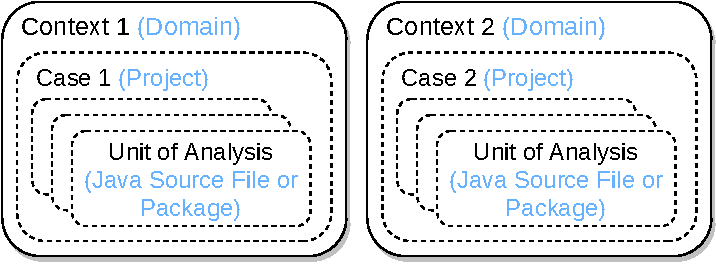
\includegraphics[width=.6\linewidth]{c5/case-design.pdf}
    \caption{The case study design using Runeson et al.'s representation \cite{Runeson2012}.}
    \label{c5:fig:case-design}
\end{figure}

\subsection{Terminology}
In the next sections, we will use the term \emph{change frequency} to indicate the number of times an artifact undergoes any kind of change in a given number of commits.
For example, if an artefact changes in 3 commits out of the 100 considered, its change frequency is $.03$.

The term \emph{change size} refers to the sum of the number of lines of code added, deleted, and/or modified to/from an artefact in a single given commit.
This is commonly referred to as \emph{code churn}.
A formal definition of how we measure changes is provided in Section \ref{c5:sec:data-collection}.

Finally, we note that we use the terms \emph{commit} and \emph{version} interchangeably. Additionally, the term \emph{release} is used when a certain commit/version is explicitly packaged and tagged for public release.

\subsection{Goal and Research Questions}
The goal of this study is to understand the impact of architectural smells on source code changes.
Using the Goal-Question-Metric approach \cite{VanSolingen2002}, the goal can be formulated as follows: 
\begin{quote}
    \itshape
    \textbf{Analyse} changes in source code artefacts \textbf{for the purpose of} understanding the impact of architectural smells \textbf{with respect to} the frequency and size of those changes \textbf{from the point of view of} software developers and architects \textbf{in the context of} open source Java software systems.
\end{quote}
By (Java) source code artefacts we mean both source code files (classes) and source code packages.

The goal can be broken down into three main research questions, as follows.
\begin{itemize}
    \item[\textbf{RQ1}] Do classes and packages with smells change more frequently than classes and packages without smells?
    \begin{itemize}
        \item[\textbf{RQ1a}] Do different smell types have a different impact on frequency of change?
        \item[\textbf{RQ1b}] Does the number of smells have a different impact on frequency of change?
    \end{itemize} 
\end{itemize}
We ask this question to shed some light on the actual relationship between the existence of architectural smells and the \emph{change frequency} of classes and packages.
Such a relationship, in case it exists, confirms that architectural smells' presence correlate with increased maintenance effort, with respect to the frequency of changes of the affected artefacts.

The two sub-questions, RQ1a and RQ1b, further explore the connection between architectural smells and change frequency by looking at how different smell types and multiple smells correlate to changes.
% This research question and its sub-questions have already been answered in a previous study by Khomh et al. \cite{Khomh2009} for code smells with interesting results. Thus it is intriguing to compare architectural smells with code smells regarding their impact.

\begin{itemize}
    \item[\textbf{RQ2}] What is the difference in the change frequency of an artefact before and after a smell is introduced?
\end{itemize}
This question aims at identifying whether the introduction of a smell impacts the \emph{change frequency} of a certain artefact.
More precisely, it provides insights on whether the presence of the smell can be related to an increased change frequency in an affected artefact.
Theoretically, one would expect that the introduction of a smell leads to an increase in the change frequency in (at least some of) the artefacts affected by the smell.
Finally, the results of this research question, in case we do find evidence of such an increase, will strengthen the findings of RQ1.

\begin{itemize}
    \item[\textbf{RQ3}] Is the size of the changes in source code artefacts affected by smells, larger than in non-affected artefacts?
\end{itemize}
This question focuses on the magnitude, or \emph{size}, of the changes made (in terms of added, deleted, and changed lines of code) to the artefacts that are affected by smells. Theoretically, these artefacts should exhibit bigger changes (thus more complex ones) because working on an sub-optimal design is harder and thus requires changing more lines of code to be maintained.
Bigger changes, in most scenarios (e.g. fixing bugs, adding features, refactoring, etc.), mean developers have spent more time to implement them, resulting in a higher amount of interest paid\cite{ElEmam2000, Mockus2000}.

We emphasize that, with these research questions we are \textbf{not seeking} to establish causality between smells and changes by any means, but rather we aim at investigating correlations. This is further explained in the Discussion section.

Finally, a replication package, containing the protocol, the data, the R scripts, and a collection of 14 plots that visualise the data, is available online\footnote{\label{ftn:repl-package}Visit \url{https://doi.org/10.5281/zenodo.4897281} to download the replication package.}.

\subsection{Analysed Projects}
To conduct our study, we selected the thirty-one projects listed in Table \ref{c5:tab:projects}. 
The inclusion criteria used during the selection of the projects were:
\begin{enumerate}
    \item Non-trivial Java projects with at least $10.000$ lines of code in the last commit; 
    \item Actively maintained and used by the community (the Contributors page on GitHub should show a consistently active development\footnote{See for example Accumulo's page \url{https://github.com/apache/accumulo/graphs/contributors} for an example of actively-developed project.});
    \item At least 3 years of active development on GitHub (or similar sites);
\end{enumerate}
During the selection process we also strove to diversify the domains of the included systems as much as possible, as indicated in Table \ref{c5:tab:projects}, as well as to increase as much as possible the period of analysis taken into consideration.
To this end, our dataset contains thirty one projects, with an average period of analysis of 11.5 years, a maximum of 22.1 years, and a minimum of 3.5 years with an average of 126.8 commits analysed per project.
Figure \ref{c5:fig:projects-versions-loc} reports the distribution of the total number of lines of code of the commits analysed for each project.

\begin{table}[]
    \centering
    \caption{Demographics of the projects analysed in this study. Note that dates refer to the period of analysis taken into consideration, not age of the system. Additionally, the categories are only indicative.}\label{c5:tab:projects}
      \begin{tabular}{m{2.5cm}|l|l|l|l|l|l}
      \toprule
      \textbf{Category} & \textbf{Project} & \multicolumn{1}{l|}{\makecell{\textbf{\# Commits} \\ \textbf{analysed}}} & \textbf{First commit} & \textbf{Last commit} & \multicolumn{1}{l|}{\makecell{\textbf{KLOC 1st-} \\ \textbf{last commit}}} & \textbf{Description}\\
      \midrule

      % Data Storage & Management
      \multirow{6}{2.5cm}{Data storage and Management} & accumulo & 99 & 23-12-2011 & 1-11-2019 & 193 - 237 & Data Storage System \\
       & calcite & 81 & 23-11-2014 & 21-5-2021 & 109 - 187 & Dynamic Data Management \\
       & cassandra & 136 & 10-4-2009 & 4-11-2019 & 36 - 178 & Distrib. NoSQL database \\
       & chukwa & 73 & 31-10-2008 & 1-4-2019 & 8 - 31 & Data Collection \\
       & jackrabbit & 155 & 24-12-2006 & 4-11-2019 & 94 - 241 & Content Repository \\
       & jackson & 93 & 6-2-2012 & 5-11-2019 & 31 - 59 & Data Binding Library \\ \midrule

      % Web  engine and tools
      \multirow{5}{2.5cm}{Web engines and Web Tools} & httpcomp. & 126 & 9-2-2006 & 3-10-2019 & 0 - 33 & HTTP Toolset \\
       & jspwiki & 186 & 25-8-2001 & 1-11-2019 & 1 - 32 & Wiki Engine \\
       & retrofit & 51 & 1-6-2015 & 18-6-2020 & 3 - 10 & Android HTTP client\\
       & spring-boot & 47 & 31-10-2017 & 31-5-2021 & 91 - 143 & Spring-based project manager\\
       & struts & 158 & 24-4-2006 & 4-11-2019 & 24 - 41 & Web Apps Framework \\\midrule

      % Search engine  
      \multirow{4}{2.5cm}{Search Engines} & elasticsearch & 49 & 16-7-2015 & 26-3-2019 & 295 - 614 & Search engine \\
       & jena & 95 & 1-6-2012 & 17-11-2019 & 209 - 348 & Semantic Web \\
       & lucene & 173 & 20-10-2001 & 3-8-2015 & 5 - 453 & Search Engine \\
       & tika & 144 & 17-8-2007 & 2-11-2019 & 2 - 63 & Content Analysis Toolkit \\\midrule

      % CI/CD Tools
      \multirow{5}{2.5cm}{Development Tools} & ant-ivy & 130 & 15-7-2005 & 2-11-2019 & 10 - 42 & Dependency Manager \\
       & jenkins & 186 & 17-12-2006 & 29-5-2021 & 14 - 125 & Automation server \\
       & jgit & 123 & 17-11-2009 & 17-11-2019 & 18 - 113 & Java implementation of Git\\
       & selenium & 132 & 16-2-2011 & 30-5-2021 & 2 - 53 & Automation web libraries\\
       & testng & 147 & 21-9-2006 & 21-10-2019 & 13 - 59 & Testing Framework \\\midrule

      % Document APIs
      \multirow{3}{2.5cm}{Document Manipulation} & pdfbox & 137 & 17-8-2008 & 3-11-2019 & 26 - 82 & PDF Library \\
       & poi & 206 & 24-3-2002 & 1-11-2019 & 19 - 99 & MS Office API \\
       & xerces2 & 189 & 3-1-2000 & 15-7-2019 & 36 - 116 & XML Library \\\midrule

      % Database APIs
      \multirow{2}{2.5cm}{JDBC Drivers} & druid & 99 & 23-6-2011 & 3-11-2019 & 42 - 85 & Alibaba JDBC Library \\
       & pgjdbc & 211 & 29-9-1997 & 4-11-2019 & 2 - 30 & PostgreSQL JDBC driver \\\midrule

      % Networking & Messaging
      \multirow{2}{2.5cm}{Networking and Messaging} & activemq & 161 & 25-1-2006 & 6-11-2019 & 61 - 177 & Message Server \\
       & mina & 120 & 22-3-2005 & 18-6-2019 & 6 - 28 & Network Framework \\ \midrule

      % Game engine
      Game Engine & libgdx & 139 & 22-4-2010 & 30-5-2021 & 23 - 222 & Game engine\\ \midrule

      % Data binding
      \multirow{2}{2.5cm}{Data Binding} & fastjson & 104 & 14-9-2011 & 5-4-2021 & 12 - 41 & Alibaba JSON data mapper \\
       & gson & 99 & 27-9-2008 & 14-5-2021 & 6 - 10 & Google JSON data mapper\\ \midrule

      Utility & guava & 83 & 11-1-2010 & 25-7-2019 & 33 - 117 & Google Core Library \\
      
      \bottomrule
      \end{tabular}%
\end{table}%

\begin{figure}
    \centering
    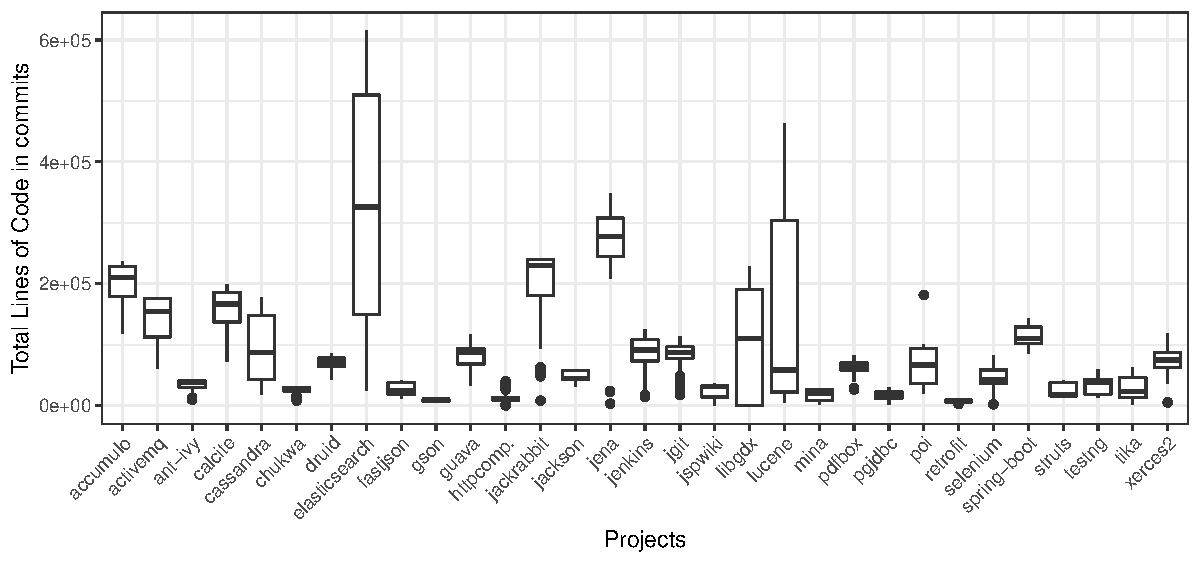
\includegraphics[width=.9\linewidth]{c5/project-version-loc.pdf}
    \caption{The distribution of the total number of lines of code of each version for each project.} \label{c5:fig:projects-versions-loc}
\end{figure}


\section{Data Collection}\label{c5:sec:data-collection}
For every system $S$ listed in Table \ref{c5:tab:projects} we analysed one commit (or version) $v$ every 4 weeks, from the first commit available in the repository to the latest on the main branch (either master or trunk).
We selected a 4-week-long interval between each commit because we wanted to ensure that the change-related metrics we selected were calculated at a meaningful level of granularity, allowing enough files to change from one commit to the next one.
Such custom intervals were used in similar contexts by previous studies \cite{Nagappan2007,Kouroshfar2015,Arcelli2019b}.
Additionally, a fixed interval between commits, avoids the introduction of bias and ensures the results are consistent across the different release rates of our projects \cite{Kouroshfar2015}. The selection of the 4-week-long interval is further discussed in the Threats to Validity Section.
The change-related data were extracted using \texttt{git diff} between each pair of consecutive commits.
The period of analysis started from the first ever commit available on the repository to the last one available as of May 2021. Next, as part of our data cleaning process, we removed the commits with no changes at the beginning and ending of a project, as these entail inactive leading and trailing periods.


For every artefact $x$, namely class $c$ or package $p$, in each commit $v$ we collected the following \textbf{\emph{independent}} variables: (1) a boolean variable denoting whether $x$ was affected by architectural smells or not, (2) four boolean variables indicating whether a certain type of smell affects $x$, (3) and an integer variable counting the total number of smell instances per smell type that affected it.
We also measure, for every artefact $x$ the changes in the system using a well-established suite of metrics provided by Elish et al. \cite{Elish2013} -- these are the \textbf{\emph{dependant}} variables in our study:
\begin{enumerate}
   \item \textbf{Change Has Occurred (CHO)}. This metric is the basis for calculating the \emph{change frequency} of an artifact. \emph{CHO} measures whether a class $c$, or package $p$, has changed or not in the current commit $v$ with respect to the previous commit $v-1$ in the dataset:
    \begin{align*} 
    CHO_v(c) = \begin{cases}
        1 & \text{if } c \text{ has changed in } v \\
        0 & \text{otherwise}
    \end{cases} &&
    CHO_v(p) = \bigvee_{c \in p}^{p} CHO(c)
    \end{align*} 
    Note that to calculate \emph{CHO} for a package $p$ (i.e. right-most formula) we do a binary sum (i.e. binary \emph{OR}) between all the elements $c$ directly contained in $p$.

    \item \textbf{Percentage of Commits a Class has Changed (PCCC)}. This metric computes the \emph{change frequency} of an artefact using \emph{CHO} and is represented as a percentage to normalise it. The metric was described and used in previous studies \cite{Arvanitou2017,Zhang2013} and is basically the \emph{FRCH} metric defined by Elish et al. \cite{Elish2013} but normalised as a percentage.
    $$PCCC^a_b(x) = \frac{\sum_{v = a}^{b} CHO_r(x)}{b-a} \times 100$$
    where $v$ is the commit for which CHO is computed, and $[a, b]$ is the interval of commit indexes considered.
    Intuitively, this metric counts the number of commits where an artefact has undergone changes and divides it by the number of commits in the period considered.

    \item \textbf{Total Amount of Changes (TACH)}. Also called \emph{change size}, or \emph{code churn}, is the sum of added lines of code (\emph{NAL}), deleted lines (\emph{NDL}), and twice the changed lines (\emph{NCL}) since the last commit\cite{Elish2013} for a given class $c$ or package $p$:
    \begin{align*}
    TACH(c) = NAL(c) + NDL(c) + 2 \times NCL(c) &&   
    TACH(p) = \sum_{c \in p}^{p} TACH(c) 
    \end{align*}
    The calculation of \emph{TACH} for packages is simply the sum of \emph{TACH} for each class $c$ directly contained in $p$.
\end{enumerate}


To collect the data, we used a combination of two tools: Arcan \cite{Arcelli2016} and ASTracker \cite{Sas2019}. Arcan collected the artefacts affected by architectural smells in each selected commit in the history of the systems directly from the source code files.
The output of Arcan is a graph file containing the dependency network of the commit analysed, including the smells detected.
The algorithms used to detect architectural smells are explained in detail by Arcelli et al. in their paper\cite{Arcelli2016}. The detection is based on the software design principles reported by Martin \cite{Martin2018} and Lippert \cite{Lippert2006}.
In short, Cyclic Dependency is detected using a Depth-First Search algorithm that visits all the nodes in the dependency graph while checking which were already visited. 
Unstable Dependency is detected using Martin's Instability metric \cite{Martin2018}: if the \emph{majority} of a package's  dependencies are less stable than itself, then it is marked as an unstable dependency smell.
Hublike Dependency is detected by simply looking at the number of incoming and outgoing dependencies a certain artefact has: if the sum of these dependencies surpasses a certain system-based threshold, then the artefact is marked as a hub.
Finally, God Component is detected using an automatically-calculated variable threshold \cite{Arcelli2015} using the distribution of the total amount of lines of code of the packages in a benchmark of over 100 systems; the packages in the analysed system are then compared with this threshold and the artefacts surpassing it are marked as God Components \footnote{See \url{https://fse.studenttheses.ub.rug.nl/19603/} for more details.}.

Arcan's results were validated in different studies. A first validation of the results of Arcan was performed on two open source projects with a precision of 100\% \cite{Arcelli2016}. 
Next, the results of Arcan were also validated in an industrial setting by two different studies: first on industrial C/C++ projects obtaining 50\% precision \cite{Martini2018} and then on industrial Java projects obtaining 70\% precision \cite{Arcelli2020}.
The precision metric was chosen as the main indicator of Arcan's performance because the true positive rate was found to be the main concern for developers during the mentioned studies.

The second tool we used, ASTracker, computed the above-mentioned change metrics and identified the elements affected by each smell.
ASTracker's main feature is to track architectural smells from one version to the next (i.e. link the same instances detected in two adjacent versions), but for this study it was only used to calculate the change metrics as stated above. To guarantee the correctness of the implementation of the change metrics, we used thorough unit testing.

At last, the Peregrine high performance computing cluster, offered by the University of Groningen, provided the computational power necessary to carry out the whole data collection process.

\section{Data analysis}\label{c5:sec:data-analysis}
\subsection{Controlling for size}\label{c5:sec:data-analysis-size}
Changes to source code files are intuitively more frequent in files of greater size (i.e. more lines of code). In fact, source code size has been empirically found to interfere with the actual findings in several cases \cite{ElEmam2001,Zhou2009}. Thus, source code size is a confounding factor in our analysis that could skew the results unpredictably and obfuscate the impact of smells on change frequency and size.
To mitigate this threat, as already mentioned in the Introduction and Related Work sections, the data analysis will include controlling for size. Specifically, we will analyse the data both by considering all artefacts (without controlling for source code size) and by grouping the artefacts (either classes or packages) into four size groups, based on their effective lines of code (LOC). This way we can compare how smells impact files of similar size.
The groups are defined as follows: Small = $[1, Q_1)$, Medium-Small (M-Small) = $[Q_1, Q_2)$, Medium-Large (M-Large) = $[Q_2, Q_3)$, and Large = $[Q_3, Q_4)$, where $Q_1$, $Q_2$, $Q_3$, $Q_4$ are the first, second, third, and fourth quartiles respectively of the distribution of the LOC of classes (or packages, when working with smells affecting packages) in a given project. This means that these values differ for each project. Table \ref{c5:tab:quartiles-loc} shows the quartiles of the LOC distribution in the whole data set.


\begin{table}[]
    \caption{Distribution of the Lines Of Code metric in classes and packages in the whole data set.}
    \centering
    \label{c5:tab:quartiles-loc}
    \begin{tabular}{@{}llllll@{}}
    \toprule
            & \textbf{0\%} & \textbf{25\% ($Q_1$)} & \textbf{50\% ($Q_2$)} & \textbf{75\% ($Q_3$)} & \textbf{100\% ($Q_4$)} \\ \midrule
    Class   & 1   & 10        & 27        & 77        & 14990 \\
    Package & 1   & 549       & 1340      & 2976      & 59074 \\ \bottomrule
    \end{tabular}
\end{table}

This approach was proposed by Aniche et al. in a previous study \cite{Aniche2018}. We adopted it as it  allows us to compare smelly and non-smelly artefacts with comparable size.
This method guarantees that all four groups have the same number of files, which is an important prerequisite to ensure that the results of the study are not skewed. Indeed, if we were to partition the files, for example, with a range of 45 LOC per group, the resulting small group (0-45 LOC) would have 200K+ artefacts, whereas the others just a few thousands. This imbalance would greatly affect the outcome. 


\subsection{RQ1 -- Do classes and packages with smells change more frequently than classes and packages without smells?}
For this RQ we statistically analyse the significance of the association between changes in affected and non-affected artefacts.
The Fisher's exact test of independence \cite{Sheskin2007} is performed on two categorical variables: in our case, these variables are CHO and whether this artefact is affected by a smell.
The input to the test is a contingency table where all the possible values of the two (categorical) variables are listed on the rows and columns of the table respectively. 
The null and alternative hypotheses of the tests (one test for each 4-month-long period considered) are:
\begin{itemize}
    \item \textbf{Null hypothesis} $H^{RQ1}_0$: artefacts affected by smells are \textit{equally} likely to be subject to changes than artefacts not affected by smells ($\pi_1 = \pi_2$)
    \item \textbf{Alt. hypothesis} $H^{RQ1}_1$: artefacts affected by smells are more likely to be subject to changes than artefacts not affected by smells ($\pi_1 > \pi_2$)
\end{itemize}
where $\pi_1$ and $\pi_2$ represent the proportions of the two categories with respect to the overall population.

To ensure the test is \emph{supported}, we need to make sure that the proportions in the contingency tables used to run the tests are not excessively unbalanced towards one category. Contingency tables are likely to be unbalanced if the time period is too small because only limited changes can happen in a certain amount of time and that time can not be enough to determine whether the correlation is present or not.
In other words, given that there are more non-changing files than changing files, a period of 1 month is likely to be insufficient for enough files to change.
Thus we aggregated our data to a 4-month granularity (rather than 1-month); this is approximately the average release rate we mined from the Git tags of our projects. We call these ``versions'' \emph{pseudo-releases}.
Thus, for each pseudo-release $v$, we test for the null-hypothesis, namely, whether there is no statistical difference in the proportions of changes for artefacts affected and not affected by architectural smells. 
This analysis will include all types of smells, both at class and package level, detected by Arcan.

The next step is to compare the percentages of pseudo-releases that do show a significant difference (accepting $H^{RQ1}_1$) and the pseudo-releases that do not show any significant difference (accepting $H^{RQ1}_0$), which will allow us to answer RQ1.
Note that we opted to perform one test per commit per project, rather than one test per project, to ensure that the imbalance in changes detected is not the result of a few change hotspots throughout the history of the system, but rather a more constant phenomenon.
The confidence level used for this test and all the following tests is equal to $\alpha = .05$.

\subsubsection{RQ1a -- Do different smell types have a different impact on frequency of change?}\label{c5:sec:rq1a-analysis}
In order to answer RQ1a, we used a logistic regression model \cite{Sheskin2007}. This kind of model allows to predict the value of a binary dependant variable given a set of multiple independent variables. 
Moreover, it can be exploited to compute the effect size between the dependant variable and each independent variable, to identify which variable influences the outcome.
In this case, we chose the CHO metric (see Section \ref{c5:sec:data-collection}) as dependant variable and the number of smell instances of each smell type $t$ as independent variables.

The hypotheses of this analysis are:
\begin{itemize}
    \item \textbf{Null hypothesis} $H^{RQ1a}_0$: the type of smells does not have an impact on the occurrence of changes of artefacts
    \item \textbf{Alt. hypothesis} $H^{RQ1a}_1$: the type of smells does have an impact on the occurrence of changes of artefacts.
\end{itemize}
The analysis was performed individually for each 4-month commit period, for all projects. Then, for each type of smell we counted the number of times that the $p$-values obtained by the logistic regression were significant.

\subsubsection{RQ1b -- Does the number of smells have a different impact on frequency of change?}
For RQ1b we used the non-parametric Mann-Whitney statistical test to check whether the average number of smells per commit in artefacts that do not change and in artefacts that do change is statistically similar.
Formally, we calculate
\begin{align*}
    changed(v) = \sum_x^{C_v}\frac{n_v(x)}{|C_v|} & & unchanged(v) = \sum_x^{U_v}\frac{n_v(x)}{|U_v|}
\end{align*}
%$$ changed(v) = \sum_x^{C_v}\frac{n_v(x)}{|C_v|}$$
%$$ unchanged(v) = \sum_x^{U_v}\frac{n_v(x)}{|U_v|}$$

where $C_v$ is the set of artefacts $x$ that changed in commit $v$, $U_v$ is the set of unchanged artefacts, and $n_v(x)$ counts the number of smells $x$ has in $v$.
 
The hypotheses for this analysis are:
\begin{itemize}
    \item \textbf{Null hypothesis} $H^{RQ1b}_0$: the number of smells in artefacts that do not change is equal to the number of smells in artefacts that do change ($\mu_{unchanged} = \mu_{changed} $)
    \item \textbf{Alt. hypothesis} $H^{RQ1b}_1$: the number of smells in artefacts that do not change is \emph{less} than the number of smells in artefacts that do change  ($\mu_{unchanged} < \mu_{changed} $).
\end{itemize}
with $\mu$ representing the mean of the populations (changed and unchanged).
Additionally, to further reinforce the findings we also check whether there is any correlation (using Spearman's $\rho$) between the number of smells an artefact is affected by and the number of changes or their size.

\subsection{RQ2 -- What is the difference in the change frequency of an artefact before and after a smell is introduced?}\label{c5:sec:rq2-analysis}
The analysis for this research question will look at the PCCC metric of a certain artefact before and after a smell is introduced in that element. We then aggregate the data per project and perform a Wilcoxon Signed-Ranks test \cite{Sheskin2007} for each project.

Formally, for every artefact $x$ affected by a smell in the lifetime of a system $S$ we compute 
$$d_S(x) = PCCC_{after}(x) - PCCC_{before}(x)$$
where $PCCC_{before}(x) = PCCC^i_k(x)$ and $PCCC_{after}(x) = PCCC^k_j(x)$ with $i$ being the commit index where $x$ first appeared, $k$ where it was first affected by a smell, and $j$ when it was last affected by a smell, or the final commit.
Artefacts with either a before or after window smaller than 5 commits were filtered out to avoid skewed data.
The values assumed by $d_S$ for the selected artefacts from $S$ are used as input for the test.

The hypotheses for this test are:
\begin{itemize}
    \item \textbf{Null hypothesis} $H^{RQ2}_0$: the change frequency of artefacts before and after a smell is introduced is the same ($\theta_{d_S} = 0$)
    \item \textbf{Alt. hypothesis} $H^{RQ2}_1$: the change frequency of artefacts after a smell is introduced is greater than before ($\theta_{d_S} > 0$). 
\end{itemize}
where $\theta$ represents the true median of the underlying population.
Additionally, using the Shapiro–Wilk test, we also test for the normality of $d_S$ to ensure we chose the appropriate statistical test.

\subsection{RQ3 -- Is the size of the changes in source code artefacts affected by smells, larger than in non-affected artefacts?}
For this RQ we want to investigate if there is a significant difference in the \emph{variance} of the size of the changes in affected versus non-affected artefacts in each commit analysed.
We look at the variance because the majority of commits have a relatively small change size, whereas few commits (e.g.  the pull requests) have a very large change size.

To determine whether there is a significant difference in these two groups (smelly vs non-smelly), we perform a Brown-Forsythe test for the homogeneity of variance \cite{Sheskin2007}.

For each commit $v$ we compute the aggregate change size (TACH metric) of changing artefacts by averaging all the change sizes for that commit.
Formally:
\begin{align*}
    smelly(v)  = \sum_{x}^{A_v} \frac{TACH(x)}{|A_v|} & & & clean(v) = \sum_{x}^{N_v} \frac{TACH(x)}{|N_v|}
\end{align*}
where $A_v$ is the set of affected artefacts in a commit $v$, and $N_v$ the non-smelly artefacts. Note that we use the term ``clean'' to indicate \textbf{non-smelly} artefacts for conciseness.

Next, we test the following hypotheses on those two variables for each project:
\begin{itemize}
    \item \textbf{Null hypothesis} $H^{RQ3}_0$: the variance in change size is equal in affected and clean artefacts by smells ($\sigma^2_{smelly} = \sigma^2_{clean}$)
    \item \textbf{Alt. hypothesis} $H^{RQ3}_1$: the variance in change size is not equal in affected and clean artefacts ($\sigma^2_{smelly} \ne \sigma^2_{clean}$)
\end{itemize}
where $\sigma^2_{smelly}$ and $\sigma^2_{clean}$ represent the true variance in the underlying populations.


\section{Results}\label{c5:sec:results}
\subsection{Relation between change frequency and smelly artefacts (RQ1)}
The results of the Fisher's tests (main question of RQ1) performed on each 4-month period of the thirty-one systems analysed are pretty straightforward when not controlling for size.
Figure \ref{c5:fig:rq1-results} reports in detail the number of 4-month periods (or pseudo-releases) where the null hypothesis was accepted, rejected, or the test was unsupported by the data.
The proportion of smelly artefacts that change is consistently higher than non-smelly artefacts that change in $82$\% of the total 4-month periods analysed in most of the projects (rejecting $H^{RQ1}_0$). In other words, \textbf{artefacts with smells do change more frequently}. For the remaining $18$\%, if we remain conservative and assume that the $11.5$\% of the unsupported tests are accepted, the smelly and non-smelly artefacts are equally likely to change (accepting $H^{RQ1}_0$).
Note that the unsupported tests are usually the ones corresponding to the pseudo-releases in the early phases of the project with a relatively little number of smells and/or changes.
We also note that these percentages hold for the majority of the projects, with six exceptions: Elasticsearch, Jena, HTTP-components, Guava, Retrofit, and Spring-boot.
These projects exhibit the opposite scenario, with more than $50$\% of the pseudo-releases featuring changes in non-smelly artefacts (neither accepting nor rejecting $H^{RQ1}_0$).
This can be at least partially explained in all six cases: they either have a very low density of smells (HTTP-components and Retrofit) or the actual proportion of smelly components that change is lower (up to 10 times) than non-smelly components that change (Elasticsearch, Guava and Jena).
\begin{figure}[t]
    \centering
    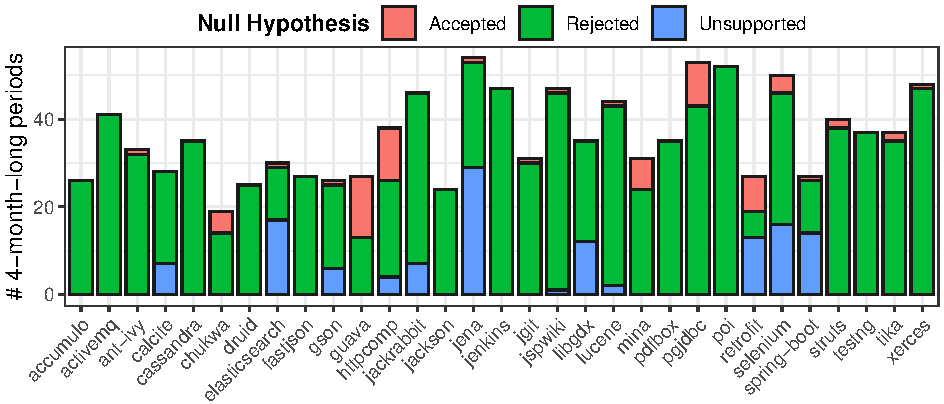
\includegraphics[width=.8\linewidth]{c5/rq1.pdf}
    \caption{Results of the Fisher's test for each project (Averages: Accepted: $6.5$\%; Rejected: $82.1$\%; Unsupported: $11.4$\%).}\label{c5:fig:rq1-results}
\end{figure}

When adjusted for size (using the lines of code - see Section \ref{c5:sec:data-analysis-size}), the results depicted in Table \ref{c5:tab:rq1-results} show that 
for \emph{Medium-Large} and \emph{Large} artefacts the null hypothesis $H^{RQ1}_0$ was rejected $66.1$\% and $78.9$\% of the times on average across all projects, respectively.
For \emph{Small} and \emph{Medium-Small} artefacts, percentages drop to $30.2$\% and $45.4$\%, respectively.
In total,  $H^{RQ1}_0$ was rejected $55.7$\% of the times and accepted $30.2$\%, while in the remaining $14.1$\% of times, the analysis was unsupported.

Ultimately, the results controlled for size do not deviate too much from the uncontrolled ones, but allow us to discern that \textbf{the larger the file, the more an artefact is likely to change if affected by a smell}.

\begin{table}
    \centering
    \caption{Percentages of rejected $H^{RQ1}_0$ per project by size group. (Averages: Accepted: $33.6$\%; Rejected $59.1$\%; Unsupported: $7.3$\%)}\label{c5:tab:rq1-results}
    \begin{tabular}{l|r|r|r|r}
        \toprule
        \multirow{2}{*}{\textbf{Project}} & \multicolumn{4}{c}{\textbf{\% P-value $< .05$}} \\
        & \textbf{Small} & \textbf{Med.-Small} & \textbf{Med.-Large} & \textbf{Large} \\
        \midrule
        accumulo & \databar{38.5} & \databar{65.4} & \databar{96.2} & \databar{100.0} \\
        activemq & \databar{78.0} & \databar{65.9} & \databar{100.0} & \databar{100.0} \\
        ant-ivy & \databar{57.6} & \databar{57.6} & \databar{90.9} & \databar{100.0} \\
        calcite & \databar{67.9} & \databar{64.3} & \databar{75.0} & \databar{71.4} \\
        cassandra & \databar{74.3} & \databar{94.3} & \databar{100.0} & \databar{100.0} \\
        chukwa & \databar{0.0} & \databar{31.6} & \databar{42.1} & \databar{63.2} \\
        druid & \databar{40.0} & \databar{84.0} & \databar{96.0} & \databar{100.0} \\
        elasticsearch & \databar{30.0} & \databar{43.3} & \databar{43.3} & \databar{43.3} \\
        fastjson & \databar{7.4} & \databar{33.3} & \databar{85.2} & \databar{88.9} \\
        gson & \databar{3.8} & \databar{0.0} & \databar{30.8} & \databar{69.2} \\
        guava & \databar{37.0} & \databar{0.0} & \databar{25.9} & \databar{29.6} \\
        httpcomp. & \databar{2.6} & \databar{13.2} & \databar{36.8} & \databar{39.5} \\
        jackrabbit & \databar{15.2} & \databar{69.6} & \databar{84.8} & \databar{84.8} \\
        jackson & \databar{33.3} & \databar{95.8} & \databar{100.0} & \databar{100.0} \\
        jena & \databar{9.3} & \databar{29.6} & \databar{38.9} & \databar{44.4} \\
        jenkins & \databar{44.7} & \databar{72.3} & \databar{95.7} & \databar{100.0} \\
        \bottomrule
    \end{tabular}
    \quad
    \begin{tabular}{l|r|r|r|r}
        \toprule
        \multirow{2}{*}{\textbf{Project}} & \multicolumn{4}{c}{\textbf{\% P-value $< .05$}} \\
        & \textbf{Small} & \textbf{Med.-Small} & \textbf{Med.-Large} & \textbf{Large} \\
        \midrule
        jgit & \databar{48.4} & \databar{77.4} & \databar{96.8} & \databar{96.8} \\
        jspwiki & \databar{31.9} & \databar{70.2} & \databar{68.1} & \databar{89.4} \\
        libgdx & \databar{8.6} & \databar{28.6} & \databar{78.3} & \databar{100.0} \\
        lucene & \databar{38.6} & \databar{47.7} & \databar{56.8} & \databar{75.0} \\
        mina & \databar{25.8} & \databar{12.9} & \databar{38.7} & \databar{67.7} \\
        pdfbox & \databar{54.3} & \databar{77.1} & \databar{94.3} & \databar{100.0} \\
        pgjdbc & \databar{24.5} & \databar{35.8} & \databar{64.2} & \databar{79.2} \\
        poi & \databar{36.5} & \databar{55.8} & \databar{92.3} & \databar{100.0} \\
        retrofit & \databar{0.0} & \databar{0.0} & \databar{3.7} & \databar{11.1} \\
        selenium & \databar{18.0} & \databar{36.0} & \databar{40.0} & \databar{62.0} \\
        spring & \databar{14.8} & \databar{3.7} & \databar{25.9} & \databar{44.4} \\
        struts & \databar{40.0} & \databar{32.5} & \databar{85.0} & \databar{95.0} \\
        testng & \databar{5.4} & \databar{5.4} & \databar{37.8} & \databar{100.0} \\
        tika & \databar{13.5} & \databar{51.4} & \databar{70.3} & \databar{91.9} \\
        xerces2 & \databar{35.4} & \databar{52.1} & \databar{56.2} & \databar{97.9} \\ \midrule
        \textbf{Avrg.} & \databar{30.2} & \databar{45.4} & \databar{66.1} & \databar{78.9} \\
        \bottomrule
    \end{tabular}
\end{table}

\paragraph{RQ1a}
The aim of answering RQ1a was to understand if the specific type of the smells affecting the artefacts has an impact on the occurrence of changes. Table~\ref{c5:tab:rq1a-results} introduces the results of the multinomial logistic regression model.
For each type of smell, it shows the proportion of the 4-month-long periods where the null hypothesis was rejected.
A large number of rejected instances means that the given type of smell has a significant effect on the dependant variable of the regression model, that is the \emph{occurrence of changes}.
The table reports all the statistically significant rates where a variable was considered relevant in the prediction of a change. Each column is a different model calibrated for that size group (or using all files in the case of `Uncontrolled').
We first notice that all the variables exhibit an increase in significance as we look at size groups of larger files.
There seems to be no particular smell type, perhaps only excluding Hublike Dependency, that provides a clear contribution to the regression model over the other types.

The results imply that, in most cases, HL is the smell that contributes the most to changes, however, there is no sufficient evidence to affirm that there is a clear distinction between different types of smell.
Thus, we conclude that we accept $H^{RQ1a}_0$ and affirm that \textbf{there is \emph{no significant difference} in the prediction power of different smell types on source code changes}.

\begin{table}
    \centering
    \caption{Results of the multinomial logistic regression in percentage of commits a variable was statistically significant in predicting a change (Rejecting $H^{RQ1a}_0$).}\label{c5:tab:rq1a-results}
    \begin{tabular}{l|r|r|r|r|r}
        \toprule
        \multirow{2}{*}{\textbf{Variable}} & \multicolumn{5}{c}{\textbf{Commits \% when variable is significant}} \\
        & \textbf{Small} & \textbf{Med.-Small} & \textbf{Med.-Large} & \textbf{Large} & \textbf{Uncontrolled} \\
        \midrule
        Cyclic Dependency   & \databar{12.2} & \databar{14.1} & \databar{20.2} & \databar{29.1} & \databar{39.7} \\
        Unstable Dependency & \databar{8.3}  & \databar{14.6} & \databar{20.6} & \databar{32.4} & \databar{29.7} \\
        Hublike Dependency  & \databar{22.1} & \databar{22.3} & \databar{26.7} & \databar{44.6} & \databar{51.9} \\
        God Component       &  --            & --             & --             & \databar{30.5} & \databar{38.5} \\
        %Lines Of Code  & \databar{20.0} & \databar{28.8}  & \databar{39.7} & \databar{62.4} & \databar{83.5} \\
        \bottomrule
    \end{tabular}
\end{table}

\paragraph{RQ1b}
Furthermore, for RQ1b, we tested whether the number of smells (including 0) affecting an artefact is an important variable contributing to its change frequency.
The test results, depicted in Figure \ref{c5:fig:rq1b-test} show that in all projects, but two (Guava and Pgjdbc), the average number of smells in changing artefacts is statistically higher than in non-changing artefacts (rejecting $H^{RQ1b}_0$) when not controlling for size.
If we consider the different size groups, the rejection rate is higher in the larger ones, whereas in the \emph{Small} group we reject $H^{RQ1b}_0$ only twice. Additionally, larger size groups also have a larger Cliff's Delta coefficient with 31 tests having $\delta > .5$ in the Large and M-Large groups against the 3 in the M-Small and Small groups, highlighting the difference in magnitude between the values of the two variables tested.

To better grasp the contrast in smell density between changing and non-changing artefacts in different size groups, Figure \ref{c5:fig:rq1b-density} plots the density (i.e. \# commits) of the (average) number of smells of these two categories.
In the figure, one can see how the average number of smells in changing and non-changing artefacts varies in the commits in our data set. When no smells affect an artefact (leftmost side of the plot), in several commits, only the smaller files change. But looking at the Medium-Large and Large files, we observe both curves shifting in shape and moving towards the right of the plot, with the changing artefacts curve growing larger and distantiating itself from the non-changing artefacts curve.
This means that \textbf{for artefacts with more smells, the larger they are, the more likely they are to change}.

Figure \ref{c5:fig:rq1b-numsmells-size-freq} shows how the change frequency varies by the number of smells affecting an artefact, with different colours representing different projects. 
As it can be noted, there is a steep increase in the number of changes as the number of smells increases from 0 to 15, before stabilizing and slightly growing towards the end of the plot\footnote{For reference, the right-most project in yellow-ish/ocra is Cassandra. Per-project plots are available in the replication package.}. 
The Spearman statistical correlation tests show that: 8 projects show a strong ($\rho \ge .7$) positive correlation; 7 show a moderate ($.5 \le \rho < .7$) positive correlation; 5 projects have a weak ($.3 \le \rho < .5$) correlation; for 2 projects there is little-to-no correlation ($ \rho <.3 $); and for the remaining 9 projects $p > .05$.

In summary, \textbf{the more smells affecting an artefact, the higher the change frequency for that artefact}. 

\begin{figure}
    \centering
    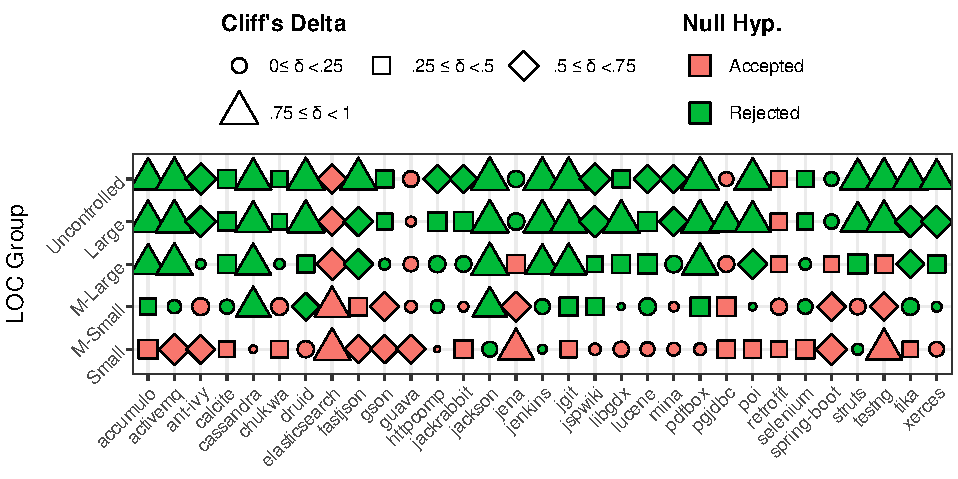
\includegraphics[width=.8\linewidth]{c5/rq1b-test.pdf}
    \caption{Mann-Whitney tests testing $H^{RQ1b}_0$ by size groups.} \label{c5:fig:rq1b-test}
\end{figure}

\begin{figure}
    \centering
    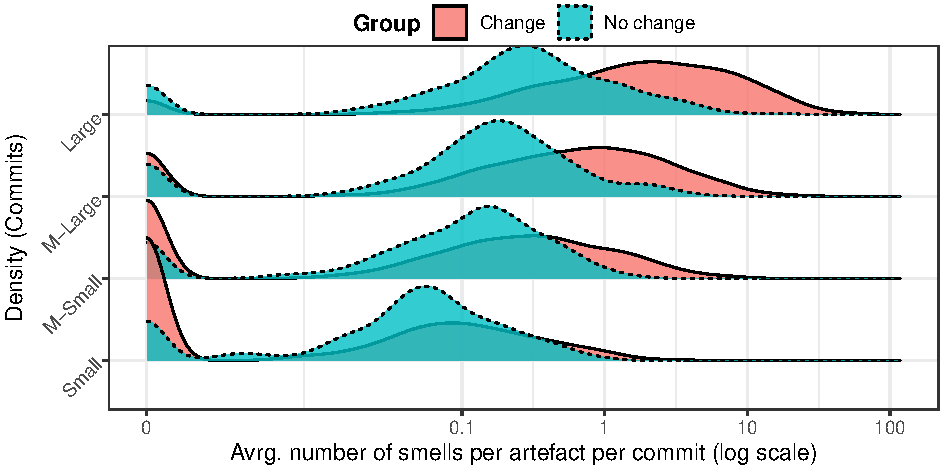
\includegraphics[width=.8\linewidth]{c5/rq1b.pdf}
    \caption{Average number of smells in changing/not-changing artefacts in all the analysed commits by size groups.} \label{c5:fig:rq1b-density}
\end{figure}
granularities
\begin{figure}%
    \centering
    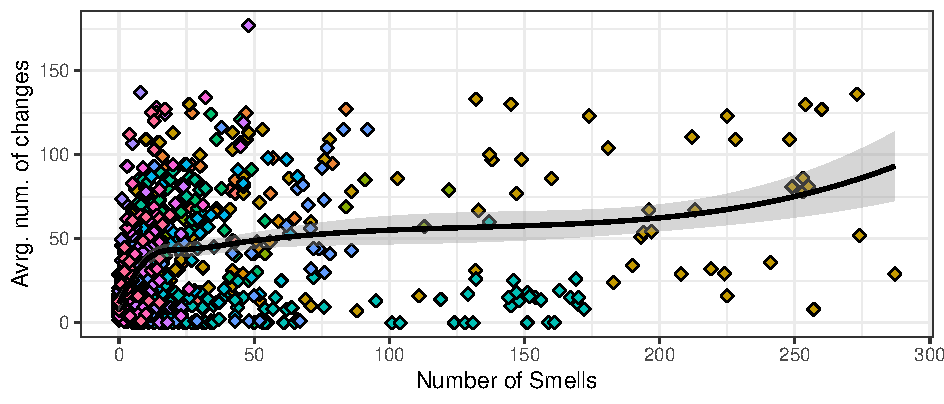
\includegraphics[width=.8\textwidth]{c5/rq1b-numOfChanges.pdf}
    \caption{Average change frequency by number of smells per project (colour-coded). LOESS regression curve shows the trend.}%
    \label{c5:fig:rq1b-numsmells-size-freq}%
\end{figure}

\subsection{Impact on change frequency after the introduction of a smell (RQ2)}
Whereas the results of RQ1 hint that changes are more likely, and more frequent, in smelly artefacts, they do not tell us anything about the effects of the introduction of a smell on the change frequency of a particular artefact throughout its lifetime.
This particular aspect is considered and tested by RQ2 through a series of Wilcoxon Signed-Ranks tests; this was confirmed to be suitable in this case because most of the projects have their $d_S$  (as defined in Section \ref{c5:sec:rq2-analysis}) function not normally distributed.
Note that we do not control for size for this RQ because this is a temporal analysis, thus there is no way to establish exactly which size category one artefact belongs to, as the LOC fluctuate over time.
The results, presented in Table \ref{c5:tab:rq2-results}, indicate that for 16 projects ($57.1\%$) there is an increase in the frequency of changes (in the PCCC metric, to be precise) after a smell is introduced. For 12 projects ($42.9\%$) instead, the opposite holds and more changes happen before the introduction of the smell. Finally, 3 projects did not contained enough samples and were ignored.

We can further inspect the distribution of $d_S$ in Figure \ref{c5:fig:rq2-density}, where we can see how the distribution of changes to the artefacts are skewed either towards the ``before'' or ``after'' the introduction of a smell side, depending on the project. Therefore, we can conclude that, \textbf{in some cases, the introduction of an architectural smell has increased the frequency of changes in the affected component}. We offer a potential explanation for the 12 projects (skewed towards the ``before'' part) that do not conform to this trend in the Discussion section, but we would like to note that 9 of the 16 projects for which we rejected the null hypothesis had $n \le 30$, whereas the accepted ones only had 6.
This means that the tests were likely accepted because of an insufficient number of samples.


\begin{table}[]
    \centering
    \caption{Wilcoxon Signed-Ranks results and the sample size (\# of artefacts) for the test ($H^{RQ2}_0$ rejected in bold). (Total: Accepted: $42.9\%$; Rejected: $57.1\%$). }\label{c5:tab:rq2-results}
    \begin{tabular}{l|r|l|r}
        \toprule
        \textbf{Project} & \textbf{P-value} & \textbf{Null Hyp.} & \textbf{Obs.}\\
        \midrule
        accumulo & $ 0.50 $ & Accepted & 11\\
        activemq & $<$ $\textbf{.01}$ & \textbf{Rejected} & 120\\
        ant-ivy & $<$ $\textbf{.01}$ & \textbf{Rejected} & 64\\
        calcite & $<$ $\textbf{.01}$ & \textbf{Rejected} & 75\\
        cassandra & $ 0.30 $ & Accepted & 178\\
        chukwa & $<$ $\textbf{.01}$ & \textbf{Rejected} & 17\\
        druid & $ 0.61 $& Accepted & 47\\
        elasticsearch & $ \textbf{0.04} $& \textbf{Rejected} & 28\\
        fastjson & $ 0.83 $& Accepted & 31\\
        gson & $ 0.50 $& Less than 10 obs. & 5\\
        guava & $<$ $\textbf{.01}$ & \textbf{Rejected} & 34\\
        httpcomp. & $<$ $\textbf{.01}$ & Less than 10 obs. & 9\\
        jackrabbit & $<$ $\textbf{.01}$ & \textbf{Rejected} & 82\\
        jackson & $ 0.28 $& Accepted & 12\\
        jena & $ 0.86 $& Accepted & 11\\
        jenkins & $<$ $\textbf{.01}$ & \textbf{Rejected} & 178\\
        \bottomrule
    \end{tabular}
    \quad
    \begin{tabular}{l|r|l|r}
        \toprule
        \textbf{Project} & \textbf{P-value} & \textbf{Null Hyp.} & \textbf{Obs.}\\
        \midrule
        jgit & $<$ $\textbf{.01}$ & \textbf{Rejected} & 42\\
        jspwiki & $<$ $\textbf{.01}$ & \textbf{Rejected} & 59\\
        libgdx & $ 0.30 $& Accepted & 98\\
        lucene & $<$ $\textbf{.01}$ & \textbf{Rejected} & 220\\
        mina & $<$ $\textbf{.01}$ & \textbf{Rejected} & 22\\
        pdfbox & $<$ $\textbf{.01}$ & \textbf{Rejected} & 103\\
        pgjdbc & $ 0.07 $& Accepted & 23\\
        poi & $ 0.25 $& Accepted & 36\\
        retrofit & $ \textbf{0.04} $& Less than 10 obs. & 4\\
        selenium & $ \textbf{0.03} $ & \textbf{Rejected} & 16\\
        spring-boot & $ \textbf{0.02} $& \textbf{Rejected} & 25\\
        struts & $ 0.05 $& Accepted & 13\\
        testng & $ 0.97 $& Accepted & 15\\
        tika & $ 0.17 $& Accepted & 33\\
        xerces2 & $<$ $\textbf{.01}$ & \textbf{Rejected} & 86\\
        & \\
        \bottomrule
    \end{tabular}
\end{table}

\begin{figure}%
    \centering
    \subfloat{{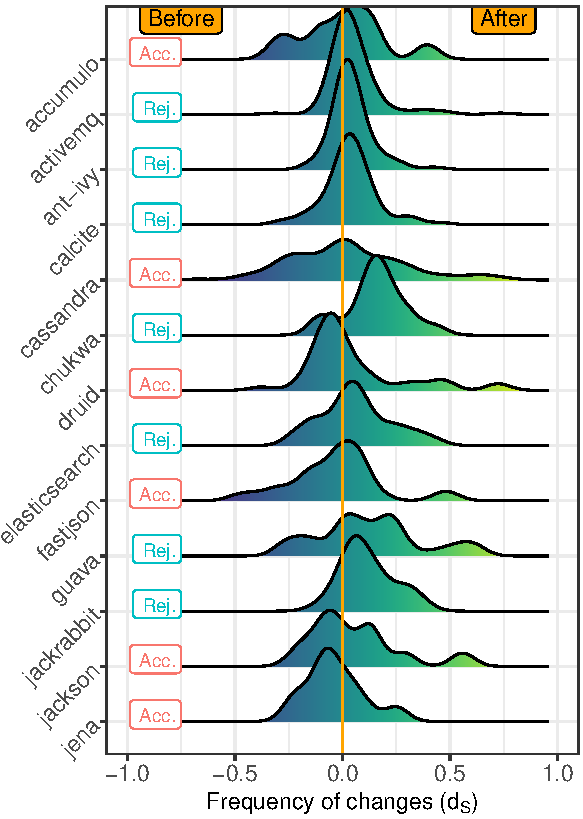
\includegraphics[width=.4\textwidth]{c5/rq2-group1} }}%
    \qquad
    \subfloat{{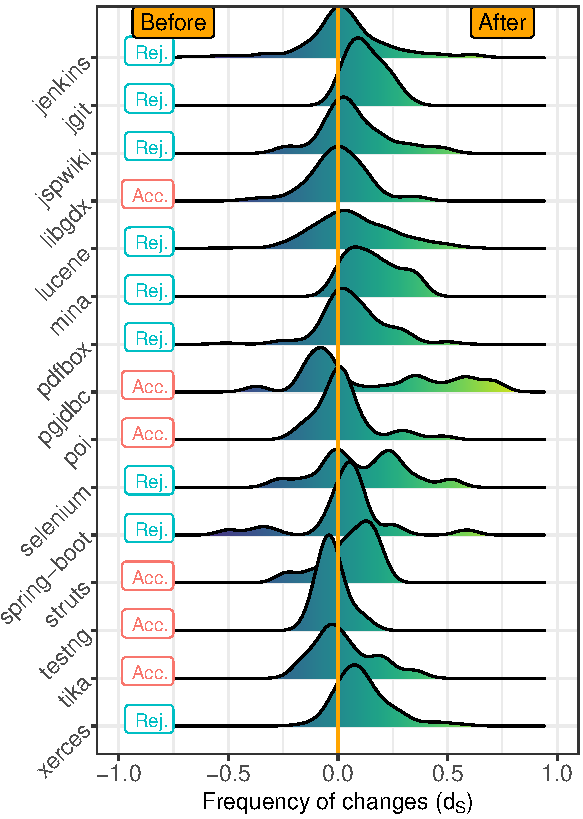
\includegraphics[width=.4\textwidth]{c5/rq2-group2} }}%
    \caption{Density of PCCC before and after the introduction of a smell ($d_S$ function).}%
    \label{c5:fig:rq2-density}%
\end{figure}

\subsection{Comparison of magnitude of changes in smelly and non-smelly artefacts (RQ3)}
For this last question, when testing the null hypothesis $H^{RQ3}_0$ on all projects, without adjusting for the size of the artefacts, we reject it for all of them -- meaning that change size (TACH metric) in artefacts affected by smells has a consistently higher variance than the non-smelly ones.
However, when controlling for the size of the affected artefacts, a different picture emerges.
The results are presented in Figure \ref{c5:fig:rq3-test}. 
Smaller classes and packages do not exhibit this pattern as consistently as the larger ones do; in fact, in \emph{Small} artefacts we note the opposite in the majority of the projects.
For \emph{Large}, \emph{M-Large}, and \emph{M-Small} artefacts the results are consistent in rejecting the null hypothesis $H^{RQ3}_0$.
This can be further visualised in Figure \ref{c5:fig:rq3-violinplots}, where the violin plots of the average change size of smelly and non-smelly artefacts in the analysed commits can be visually compared for each size group. The more elongated the shape of the violin, the larger the variance in the corresponding group.
By observing this figure, we note that the change size in smelly artefacts tends to increase (the violin shifts upwards) as the size of the artefacts increases. In stark contrast, the violin shapes of the non-smelly group are surprisingly similar across the four different groups; this contrast highlights the impact of smells on affected artefacts w.r.t. change size. 

Hence, both visual analysis and statistical tests converge to the same conclusion that \textbf{smelly artefacts undergo changes of higher magnitude than non-smelly artefacts, especially in larger artefacts}.
More precisely, smelly artefacts have an average change size (TACH) across all the projects of 1608, whereas non-smelly artefacts settle at 109. The difference is one order of magnitude higher in smelly artefacts; we note that the smelly artefacts also have a higher variance.

\begin{figure}
    \centering
    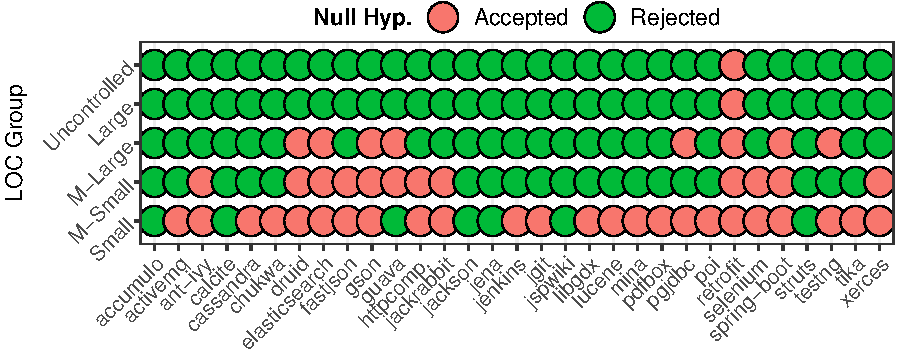
\includegraphics[width=.8\linewidth]{c5/rq3-test.pdf}
    \caption{Brown-Forsythe tests results by size groups for $H_0^3$.}\label{c5:fig:rq3-test}
\end{figure}

\begin{figure}
    \centering
    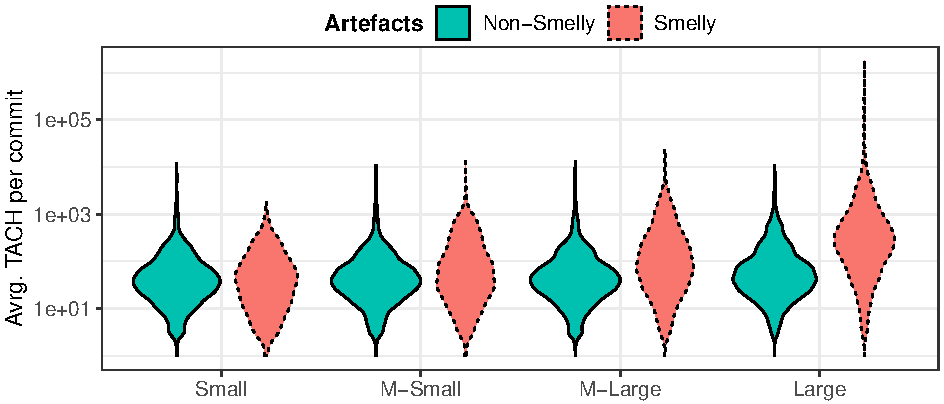
\includegraphics[width=.8\linewidth]{c5/rq3.pdf}
    \caption{Violin plots of the distribution of the average change size (TACH metric) in the analysed commits grouped by  smelly and non-smelly artefacts (log scale).}\label{c5:fig:rq3-violinplots}
\end{figure}


\section{Discussion}\label{c5:sec:discussion}
In the following section we discuss and elaborate on the results presented above.

From the obtained results, we have empirically confirmed that architectural smells (at least the ones considered for this study), exhibit a \emph{correlation} with the \emph{change frequency} and \emph{change size} of the artefacts they affect, and especially the larger artefacts.
As stated previously, our goal was to seek and establish \emph{correlation}, rather than \emph{causality}.

The results from RQ1 show that artefacts affected by at least one smell exhibit more changes than artefacts without smells. We also saw that as the number of smells increases, so does the likelihood of the affected artefact to change. 
Interestingly, we found evidence suggesting that the four different types of smells that we studied affect change frequency in a similar way. 
Theoretically speaking, the main drawback associated with the UD smell type \cite{Arcelli2016} is an increased likelihood to change caused by a low stability of the artefacts it depends upon \cite{Martin2018}.
Indeed, while we observed that UD-affected artefacts have an increased change frequency, we also expected them to have a higher change frequency than artefacts affected by the other smell types. However, this is not what we observed, as all four smell types seem to have a similar effect on change, with HL surpassing UD in fact.
The HL smell was hypothesised to be quite prone to propagate changes due to its numerous dependencies which increase the likelihood that a change propagates to the central component before rippling to the components depending on it (see related work \cite{Sas2019} for further information).
Given this theoretical description, we would predict that changes may propagate within the structure of HL smells, but we did not expect it to deviate from the other smell types and surpass UD.

%Overall, the implications of these findings are that architectural smells (regardless of their type) are quite likely to increase the maintenance effort required to maintain a software artefact. 
%In other words, they increase the \emph{architectural technical debt interest} paid over time by developers.
%This means that smelly artefacts result in \emph{reduced productivity} and a \emph{deterioration of quality} over time with respect to the non-smelly artefacts in the system. 

The results of RQ2 show an increase in change frequency \emph{after} the introduction of a smell.
This finding implies that the introduction of a smell leads to an increase in the effort developers spend on the particular artefact(s) affected by that smell compared to the period of time that artefact was not affected by any smell. 
Note that change frequency and size were used to estimate the effort spent by a developer in previous studies too \cite{Sjoberg2013,Olbrich2009,Nugroho2011}.
Nonetheless, it is interesting to note that this result is not valid for all of the projects considered, and in some cases the opposite situation occurs.
We conjecture that this result is highly dependant on how development teams decide to implement new functionality in the system.
If developers reuse existing classes, than these classes are likely to require changes for a longer period of time, and especially after a smell affects them (as seen from our results).
If developers do not reuse existing classes and implement a new functionality in new classes and packages, then old and smelly classes are less likely to be changed, because they serve their purpose as they are without requiring further changes.
%Basically, systems that require, for compatibility purposes, to expose old functionality to the user, even years after it is officially unsupported, or deprecated, might show a change frequency denser in the ``before'' side of the plot: there are parts of the system that were changed a lot until they were released but subsequently stopped changing (without removing the smells affecting them).
More generally, in the ``old'' features of a system, very little maintenance effort is spent on good design and architecture, e.g. by refactoring smells; this means that components affected by smells rarely get changed.

A perfect example of this is provided by the project PgJDBC.
PgJDBC, among other projects, has a package named ``v2'', suggesting that functionality for the previous release (``v1'') is implemented separately in a different package.
The classes implementing the functionality for the previous release are thus no longer extended and therefore they no longer change, but they are still kept in the repository in order to support legacy functionality.
Assuming that at least some of these classes were affected by smell, the resulting effect is that their change frequency after the smell was introduced is close to zero.
Moreover, given that these are open source projects, we cannot assume that they undergo constant development, and changes in the popularity of a project may influence how many pull requests, commits, and changes are performed. 
Ultimately, these two factors greatly influence the variability in the results obtained from RQ2.

With the obtained results from RQ3 there is additional evidence to support that developers spend \emph{more time} on smelly artefacts, where we noticed a consistently larger change size -- again, especially in the larger files. This is especially true in pull requests commits, the type of commits where usually new functionality, or big bug fixes, are introduced. This result becomes even clearer when observing Figure \ref{c5:fig:rq3-violinplots}: there is a strong contrast between the constant change size in non-smelly artefacts across the four different size groups, vs. the increasing change size in smelly artefacts. This clearly shows the spending of extra effort to perform changes in smelly artefacts.

Putting together the results of all the three research questions, we conclude that developers are not only compelled to make \emph{more frequent} changes to smelly artefacts, but also to make \emph{larger} changes. Ultimately, if we assume that change is a proxy of the effort spent maintaining the components affected by smells \cite{Sjoberg2013,Olbrich2009}, the technical debt interest of those components is increased by two factors: change frequency and change size.
An important caveat is that these findings do not include any input from the actual developers, therefore, further research is required in order to understand the full extent to which architectural smells perturb development activities from the perspective of software practitioners themselves.
For the time being, we can conclude that architectural smells constitute a \emph{high risk}, as their accumulation can increase technical debt interest to un-sustainable levels.

A common trend in our results is that smelly \emph{Large} and \emph{Medium-Large} smelly files exhibit statistically different patterns in change frequency and size in contrast to the \emph{Small} and \emph{Medium-Small} groups.
It is interesting to explore why this happens mostly in these size groups. 
The main reason is that GC and HL are defined based on the number of lines of code or incoming and outgoing dependencies of the affected artefact. Namely, they \emph{cannot} affect small artefacts by definitions. 
Smaller artefacts can however still be impacted by a HL smell if they depend on the hub (central artefact), because change may propagate to them from the hub.
This difference between smaller and larger files has a clear implication for researchers: we advise the development of better prioritisation methods for refactoring architectural smells by prioritising smells affecting larger artefacts; these are the ones where developers pay the most technical debt interest.

Finally, some of the findings that emerged from this study match what Oyetoyan et al. \cite{Oyetoyan2015} and Le et al. \cite{Le2018} have found in their own works.
Specifically, our results from RQ1 match what Le et al. \cite{Le2018} found, namely the average number of changes in smelly files is higher than in non-smelly files (see Figure \ref{c5:fig:rq1b-numsmells-size-freq}). On top of that, we have also shown how the number of changes positively correlates with the number of smells (RQ1b).
Answering RQ1a instead, we have noted among others, that potentially \emph{not all types of cycles} are impactful on changes. This corroborates what Oyetoyan et al. \cite{Oyetoyan2015} found about Cyclic Dependencies, i.e. certain types of cycles do not have an impact on changes. However, we did not investigate precisely which category of cycles does so and neither if they affect neighbour artefacts; we consider this future work.

\section{Study Limitations}\label{c5:sec:limitations}
The identified limitations of this study are described in terms of \emph{reliability}, \emph{external validity} and \emph{construct validity} as described by Runeson et al. \cite{Runeson2012}. Internal validity was not considered as we did not examine causal relations \cite{Runeson2012}. % We might need to address it anyway

\subsection{Construct validity}
Construct validity concerns to what extent this study is measuring what it is claiming to be measuring \cite{Runeson2012}.
To ensure construct validity, we adopted the well-known case study design guidelines provided by Runeson et al. \cite{Runeson2012} and iteratively revised the protocol during the duration of the study.
Thus, the data collection and analysis processes were meticulously planned and implemented to ensure that the final results would answer precisely the three main research questions of interest of this study.

One concrete threat to construct validity is the arbitrary selection of the 4-week interval between the analysed commits.
While the selection of this particular interval was computationally convenient (i.e. more commits would pose higher requirements for processing time), in the more active projects this time interval might have caused the loss of information for frequency-related metrics. For instance, a class might have changed several times during the course of 4 weeks, but we only count it is as one big change.
As a result, the coarse-grained frequency data may have impacted the analysis, and thus the results, of RQ2.
Additionally, this interval might clash with the culture of each development team in pushing changes to the central repository and the size of those changes.
However, the very selection of this particular interval also partially mitigated this risk, if we compare our study with related work, where most studies \cite{Le2015, Le2018, Khomh2012} use time in-between releases, which is usually longer and more susceptible to the risks mentioned above.

Similarly, the pseudo-release data aggregation we performed for RQ1 might be incorrect even though it is based on empirical evidence. The problem is that we used the date the Git tag was added, which might not match the official release date of that release.
To mitigate this risk we manually inspected all the dates and ensured they were reasonable and matched the versions' numbering order (e.g. v1.1 comes before v1.2 and their dates match such order).
Tags with different release numbers but with the same date were removed.

Another threat to construct validity is related to our use of change frequency and size as indicators of technical debt interest.
The same indicators have been used in previous studies \cite{Ampatzoglou2018,Nugroho2011}, as there is no way to directly measure technical debt interest. However, it is important to keep in mind that they are only proxies and the actual interest paid by developers might vary significantly.
Thus, assuming that an increase in change frequency and size corresponds to a \emph{direct} increase in technical debt interest paid by the development team while implementing new features, or making changes to the code base, is not always correct. 
The more frequent and bigger changes required to implement those features may be a result of the inherent difficulty of implementing the features themselves, or even other external factors.
On the other hand, it is also unlikely that \emph{all} the new features and changes are characterised by inherently-difficult elements to design and implement.

% Commented out to save space
% Finally, the last threat to construct validity we identified is the selection of our dependant variables: the change metrics.
% The risks are: (a) the metrics selected are not the best for this task, and (b) our own implementation for these metrics is incorrect.
% We mitigated the former risk by relying on a well-established suite of change metrics \cite{Elish2013} that has been also used in several other studies.
% For the latter risk, we carefully developed unit tests to guarantee that our implementation is as close as possible to the optimal one.

\subsection{External validity}
This aspect of validity reflects to what extent the results of this study can be fitted to the whole population of projects considered and relatable contexts.

Two threats have been identified in this case.
The first one involves the types of projects we selected for our study.
While all of them are open source projects, eighteen of them are projects from the Apache Foundation and only thirteen are non-Apache projects.
The imbalance is caused by the fact that most Apache projects have a very long and consistent history, which made them more likely to be adopted for our analysis.
We decided to mitigate this aspect by diversifying as much as possible the application domains of the selected projects.
Moreover, we collected our data from thirty-one projects, considerably more than what had been done by previous, similar studies (i.e. \cite{Le2015} used 14 projects; \cite{Le2018} used 8 projects, and \cite{Oyetoyan2015} used 12 projects), thus strengthening external validity.

The other threat to external validity concerns the architectural smells we used for our analysis.
It is very hard to generalise the results to other architectural smells and it is probably not possible to do so with enough confidence for every type of smell. This very much depends on the type of smell and the detection strategy for that smell. Therefore we cannot claim any generalisation of our results to other architectural smells.

\subsection{Reliability}
Reliability is the aspect of validity focusing on the degree to which the data and the analysis depend on the researchers performing them.

All the tools and the data used in this study are freely available online (see related studies and Footnote \ref{ftn:repl-package}) to allow researchers to study or replicate our results using the same data or even a different set of projects.

The intermediary findings and data analysis steps were all inspected and discussed by all the authors of this paper to ensure their reliability.
Moreover, similar data collection and analysis techniques have been also used in previous studies on code smells (e.g. \cite{Khomh2009}) and architectural smells (e.g. \cite{Le2018}), assuring that it is indeed possible to do this type of analysis for these types of artefacts.

\section{Conclusions and future work}\label{c5:sec:conclusion}
The present study has thoroughly investigated the relationship between a set of four architectural smells and the changes in the affected components.
In total, thirty-one projects, adding up to a total of 360 years of development and  over 305 million lines of code, were statically analysed and then statistically tested against our hypotheses.

The main findings of this case study show that: (1) artefacts affected by architectural smells change more frequently than non-smelly artefacts; (2) the type of the smell does not have a significant correlation with changes; (3) the more smells affect an artefact the more likely it is to change; (4) the change frequency of an artefact increases after the introduction of a smell in the majority of the systems; and (5) the size of changes is significantly higher in smelly artefacts than in non-smelly ones.
These findings are especially valid for artefacts belonging to the \emph{Medium-Large} and \emph{Large} size groups.
We thus concluded that architectural smells are very likely to be associated with an increase in the technical debt interest developers pay each time they work on artefacts affected by smells.

Given the results obtained from our RQs, it would be interesting to explore how the presence of architectural smells is perceived by the very developers and architects of a software system.
More specifically, a natural continuation of RQ1 is to investigate if practitioners do perceive that affected components are more prone to changes than non-affected components and whether there is any difference, in this regard, between different types of smells.
Concerning RQ2, it would be interesting to explore how the introduction of a smell is perceived, what lead to the introduction of the smell, and whether developers were aware of it.
Finally, for RQ3, a possible research direction is to understand whether the difference measured in our study has a perceivable impact by developers and architects; in other words, to study how big changes must be in order to make a difference in the effort perceived.


\section*{Acknowledgments}
We would like to thank the Center for Information Technology of the University of Groningen for their support and for providing access to the Peregrine High Performance Computing cluster.

This work was supported by the European Union's Horizon 2020 research and innovation programme under grant agreement No. 780572 SDK4ED (\url{https://sdk4ed.eu/}), as well as ITEA3 and RVO under grant agreement No. 17038 VISDOM (\url{https://visdom-project.github.io/website/}).


% Paper 5 - 
\setlength{\headheight}{1.2cm}
\renewcommand{\publ}{\flushleft\footnotesize{This chapter has been submitted to a journal.\\[0.1cm]}}

\chapter{An architectural technical debt index based on machine learning and architectural smells}
\label{chap:6}
\epigraph{\emph{Simplicity is a great virtue but it requires hard work to achieve it and education to appreciate it. And to make matters worse: complexity sells better.}}{--- Edsger Wybe Dijkstra}

\begin{Abstract}
	A key aspect of technical debt (TD) management is the ability to measure the amount of principal accumulated in a system.
    The current literature contains an array of approaches to estimate TD principal, however, only a few of them focus specifically on architectural TD, and none of these are fully automated, freely available, and thoroughly validated.
    Moreover, a recent study has shown that many of the current approaches suffer from certain shortcomings, such as relying on hand-picked thresholds.
    
    In this paper, we propose a novel approach to estimate architectural technical debt principal based on machine learning and architectural smells to address such shortcomings.
    Our approach can estimate the amount of technical debt principal generated by a single architectural smell instance.
    To do so, we adopt novel techniques from Information Retrieval to train a learning-to-rank machine learning model that estimates the severity of an architectural smell and ensure the transparency of the predictions.
    Then, for each instance, we statically analyse the source code to calculate the exact number of lines of code creating the smell.
    Finally, we combine these two values to calculate the technical debt principal.
    
    To validate the approach, we conducted a case study and interviewed 16 practitioners, from both open source and industry, and asked them about their opinions on the TD principal estimations for several smells detected in their projects.
    The results show that for 71\% of instances, practitioners agreed that the estimations provided were \emph{representative} of the effort necessary to refactor the smell.
\end{Abstract}

\section{Introduction}\label{c6:sec:Intro}
The technical debt (TD) metaphor borrows the concepts of \emph{principal} and \emph{interest} from the financial domain and uses them to convey key software maintenance concepts.
In particular, debt principal indicates the effort required to \emph{fix} a current, non-optimal solution, whereas debt interest indicates the recurrent effort necessary to \emph{keep maintaining} it \cite{Avgeriou2016}.
As an example, consider a portfolio management system that requires massive revisions in order to accommodate for the changes required by the customer\cite{Cunningham1992}. The interest represents the recurrent costs of making the revisions, whereas the principal is the cost of completely replacing the solution with a new one that would allow these changes to be seamless.

The importance of managing TD is ever increasing, especially for architectural TD (ATD), as architectural decisions were found to be the greatest source of TD faced by practitioners \cite{Ernst2015}.
A key part of managing TD is to be able to \emph{measure} the amount of TD principal incurred by an application, but this has not yet been effectively addressed in the state of the art.
Theoretically, the problem of measuring the TD principal requires defining a function that transforms maintenance-related data points (metrics, smells, violations of rules or principles, etc.) into a single number representing the overall effort required to fix them.
Over the past years, several studies proposed approaches to estimate the amount of debt principal accrued by an application \cite{Khomyakov2020,Avgeriou2021}, both at the architectural level and at code or design levels; however, most of these studies relied on techniques that have known shortcomings and resulted in estimation functions that were not \emph{thoroughly} validated \cite{Khomyakov2020}.
A common weakness shared by many of these studies is the use of hand-picked thresholds or relying on benchmarks that include arbitrary systems (of arbitrary size, domain, etc.) to determine these thresholds (see Section \ref{c6:sec:related-work} for more details).
Moreover, while some of these approaches are fully automated, they are no freely-available implementations that can be used by others to replicate the results obtained.

In this paper, we propose a novel approach to estimate ATD principal, called \textbf{\emph{ATDI}}, by adopting machine learning (ML) to overcome the aforementioned shortcomings of existing approaches.
The main advantage of using ML over thresholds or benchmarks is that ML does not require picking these manually; the model will automatically deduce these from the data.

In our approach, we use architectural smells (AS) as the main proxy for measuring ATD.
AS represent decisions that violate design principles and result in undesired dependencies, overblown size, and excessive coupling \cite{Lippert2006,Garcia2009} among the classes and packages of a system.
The main advantage of using AS as a proxy for ATD is that we can estimate the amount of principal each AS contributes to the system. 
This provides a benefit over simply using metrics as proxies for ATD because using AS is: a) \textbf{actionable} as practitioners can make prioritisation decisions using AS; and b) \textbf{targeted} as practitioners know exactly what the problem is, where it is, and how it should be addressed.
The main disadvantage of using AS is that they are but a part of all the possible forms that ATD can assume, therefore it is not guaranteed that all of the ATD principal is represented.
Nevertheless, AS are the most common form of ATD studied in the literature \cite{Verdecchia2018}, they have been recognised as particularly problematic in industry \cite{Arcelli2020,Sas2021b}, and  they have been used by other approaches in the literature as proxies for estimating the whole ATD principal \cite{Xiao2016,Roveda2018}. 
Further details on the choice of AS as a threat to validity are discussed in Section \ref{c6:sec:threats-to-validity}.

Our approach, uses ML to calculate the severity of each AS instance (i.e. how harmful it is to Maintainability) and then \emph{combines} it with a precise static analysis of the source code to determine the lines of code responsible for the smell (which we use to gauge the size of the smell within the system); this combination is used to calculate the ATD principal as an \emph{index}.
To train the machine learning model, we create a data set using techniques from Information Retrieval to compare AS and rank them by their severity.
The results of the training show that the ML model can successfully rank AS by their severity with a \textbf{high degree of accuracy} by achieving a .97 of $NDCG$, the de facto standard metric used to evaluate the type of ML model we used in our approach (see Section \ref{c6:sec:perf-metric} for details).
Moreover, to ensure the predicted severity is justified (e.g. not biased by a variable irrelevant to a specific smell) and \textbf{transparent}, we employ a state-of-the-art technique, called SHAP \cite{Strumbelj2014}, to visually analyse a small sample of predictions.
The results show how exactly the considered variables contribute to the predictions.

After ensuring the ML model is predicting severity correctly, we \textbf{validate} the output of the whole approach. 
We inspect whether the estimations provided by our approach are actually relevant to developers by checking whether they are \emph{representative} of the repayment effort perceived and \emph{meaningful} with respect to each other (e.g. this smell requires twice the effort to refactor than this other smell, and has a double ATDI value).
To this end, we interview \textbf{16 practitioners} from both the open source and industrial world.
Each interviewee is shown a number of AS instances in their own systems, as well as the respective ATD principal estimation provided by our approach.
In 71\% of the cases, interviewees totally agree with the estimations provided by our approach and deem them representative of the effort necessary to repay the debt.

This paper's structure is as follows:
Section \ref{c6:sec:AS} summarises the theory of architectural smells and the tool used to detect them; Section \ref{c6:sec:approach} introduces the approach we developed to estimate ATD principal as an index; Section \ref{c6:sec:study-design} elaborates on the case study design, including the data collection and analysis methodologies; Section \ref{c6:sec:descriptive-statistics} presents some descriptive statistics about ATDI; Sections \ref{c6:sec:rq1-results} and \ref{c6:sec:rq2-results}  present the results of the two research questions; Section \ref{c6:sec:discussion} discusses possible implications of the results for researchers and practitioners; Section \ref{c6:sec:threats-to-validity} describes the threats to the validity of this study and how they were mitigated; Section \ref{c6:sec:related-work} lists the related work and compares it with the results obtained by this study; and finally, Section \ref{c6:sec:conclusion-fw} concludes the paper and lists possible future work opportunities.


\section{Architectural smells}\label{c6:sec:AS}
The AS considered in this study are the following 4 types: Cyclic Dependency (CD), Unstable Dependency (UD), Hublike Dependency (HD), and God Component (GC).
A complete description of architectural smells is available in Chapter \ref{c2:sec:arch-smells}.
The description of the tool used to detect them, \textsc{Arcan}, is available in Chapter \ref{c2:sec:arcan}.

\subsection{Smell characteristics}
An architectural smell \emph{characteristic} is a property or attribute of an architectural smell instance \cite{Sas2019}. 
An architectural smell \emph{instance} is a concrete occurrence of a type of architectural smell.
For each architectural smell type, one can measure different characteristics.
In this work, we are going to use architectural smell characteristics as features (i.e. inputs) for a machine learning model (more details in Section \ref{c6:sec:calculating-severity}).
The characteristics considered in this work are described in Table \ref{c6:tab:characteristics}.

\begin{table}[tbp]
    \footnotesize
    \centering
    \caption{Architectural smell characteristics relevant in this study.}\label{c6:tab:characteristics}
    \begin{tabular}{p{0.25\linewidth}|p{0.69\linewidth}}\toprule
        \textbf{Name} & \textbf{Description} \\ \midrule
        Size & The number of artefacts affected by the smell. \\
        Number of edges & The number of dependency edges among the affected artefacts. \\ 
        PageRank & The importance of the artefacts affected by the smell within the dependency network of the system \cite{Roveda2018}. \\
        Affected Type & The type of the affected artefact (i.e. either class or package) \\
        PCT Depth* & Depth refers to the number of packages that are an ancestor of the affected element in the system's package hierarchy (i.e. the PCT) \cite{Laval2012}. \\
        PCT Distance* & The number of packages that need to be traversed in the PCT to reach an affected element of the smell starting from another affected element \cite{Laval2012,AlMutawa2014}.\\
        Shape & (for CD only) The shape of a cycle: tiny, circle, chain, star, clique (from \cite{AlMutawa2014}). \\
        Instability gap & (for UD only) Is the difference between the instability of the main component and the average instability of the dependencies less stable than the component itself \cite{Arcelli2016}. \\\midrule
    \end{tabular}
    \scriptsize{*Since every smell affects multiple elements, and PCT metrics are calculated individually on the classes and packages affected by the smell, we aggregate them as a mean and standard deviation.}
\end{table}

\section{The approach}\label{c6:sec:approach}
This section describes the approach we designed to calculate an architectural technical debt index, or ATDI.
As discussed in Section \ref{c6:sec:Intro}, our approach is based exclusively on architectural smells (AS) and does not consider other types or forms of technical debt. 

\subsection{Indexes and cost estimates}
Theoretically, technical debt (TD) principal is defined as the \emph{cost} necessary to develop a better solution than the currently implemented one \cite{Avgeriou2016}, easing future maintenance and evolution efforts.
Similarly, architectural technical debt (ATD) principal refers to the same concept, but focuses on architectural solutions only.
Several tools, both commercial and open source \cite{Avgeriou2021,Khomyakov2020}, claim to estimate the cost to repay the TD principal of a software system using just source code artefacts.
In practice, however, calculating the exact cost of remediation is a rather ambitious task, as several factors -- both internal and external to the codebase and the company -- may influence it and vary depending on context, organisation and country \cite{Murillo2021,Rios2020,Rios2018}.
If these are not taken into account, the estimate could be imprecise and not reflect the actual cost. 
An index, on the other hand, is not associated with an exact cost, but rather it correlates with the \textbf{\emph{effort}} necessary to remediate the technical debt incurred by the current solution.
It also does not make any assumptions regarding the cost of development, thus avoiding misleading engineers and misrepresenting the actual costs.
Therefore, we opted to treat the ATD principal calculated through our approach as an index, rather than as an estimation of the cost. 

The importance of choosing an index over a cost estimate emerged during the design of our approach when we received feedback on the matter from two industrial experts. 
Both experts suggested to avoid a cost estimation as this would spark unnecessary discussion and create controversy and confusion among the developers, architects, and managers who would have different opinions, ultimately leading to distrust against the provided values.
Note that this anecdotal evidence is put to the test by the validation process described in the study design section (Section \ref{c6:sec:study-design}).

To sum up, we do not aim at estimating the \emph{cost impact} of technical debt \cite{Avgeriou2016}, but only the \emph{effort required} to fix the current solution \cite{Avgeriou2016} expressed as an index. 
Using an index over a monetary estimation allows for a more concise and unbiased representation of the effort necessary to remediate the incurred TD. 
Related work from Section \ref{c6:sec:related-work-atd} and Table \ref{c6:tab:rw-comparison} show that this is also a common choice in the literature when estimating ATD principal.

\subsection{Definition}\label{c6:sec:approach-definition}
The simplest and most intuitive way of estimating the ATD index based on AS is by summing up the individual indexes of each smell\cite{Ampatzoglou2018}.
This is the solution adopted by previous studies as well \cite{Letouzey2010,Curtis2012,Marinescu2012,Roveda2018} and (1) allows users to quickly understand the impact of one instance on the overall value of the index, and (2) it resonates with the financial metaphor, where the total amount of debt is the sum of all the debts.

Formally, we define the ATD principal index as
\begin{equation}\label{c6:eq:atdi}
    ATDI(P) =  \sum_i^{S_P} ATDI(x_i)
\end{equation}
where $x_i$ are the architectural smells $S_P$ detected in the project $P$.
This value can be normalised by the size of the project $P$ in lines of code to obtain the density of ATDI per 1000 lines of code, to allow us to compare values obtained from different projects
\begin{equation}\label{c6:eq:atdi-normalised}
    ATDI_{density}(P) = \frac{ATDI(P)}{LOC(P)} \cdot 1000
\end{equation}

The index of a single smell is calculated as the product of: 
\begin{equation}\label{c6:eq:atdi-smell}
    ATDI(x_i) = s(x_i) \cdot m(x_i)
\end{equation}
\begin{enumerate}[label=\alph*)]
    \item \textbf{\emph{Severity}}, calculated by the function $s : S_P \rightarrow  [1, 10]$. \emph{Severity} was used consistently in previous studies to estimate TD principal \cite{Roveda2018,Marinescu2012,Curtis2012}. In our case, we adopted Marinescu's \cite{Marinescu2012} approach to define severity in the range $[1, 10]$ with higher values representing more severe smells\footnote{There is also a more practical reason described in Section \ref{c6:sec:calculating-severity}.};
    \item \textbf{\emph{Extent}}, calculated by the function $m : S_P \rightarrow  \mathbb{N}_{\ge 1}$ and defined as the number of the lines of code that contribute to the creation of the smell, giving an estimation of its size within the system. The \emph{extent}, or number of lines of code, was used for estimating the amount of effort in previous studies on technical debt \cite{Chatzigeorgiou2015,Kamei2016,Nugroho2011} and non-technical debt related work as well as a proxy of complexity \cite{Morasca2001, Kitchenham2004}. 
\end{enumerate}

The definition from Equation \ref{c6:eq:atdi-smell} allows us to model the intuition that \emph{more severe smells are more detrimental to maintainability} \cite{Roveda2018} and \emph{more extended smells require more effort to be removed} \cite{Nugroho2011}. 

More details on the information used by previous approaches and existing tools to calculate their indexes are summarised by Avgeriou et al. and Khomyakov et al. \cite{Avgeriou2021,Khomyakov2020}.
In the following two sub-sections we elaborate on the definition of the two concepts, i.e. severity and extent.

\subsubsection{Defining severity}\label{c6:sec:approach-definition-severity}
In software engineering, the term \emph{severity} is commonly used to describe how harmful a certain type of issue (e.g. architectural smells) is with respect to (w.r.t) a certain quality attribute (e.g. Maintainability).
Severity is used to gauge the impact of different instances of the same type of smell and decide which one is more harmful to the maintainability of the system \cite{Marinescu2012}.

Similarly to the case of code smells \cite{Arcelli2017b, Arcelli2015b} and design flaws \cite{Marinescu2012}, the severity of an architectural smell is determined by the properties of the structure of the smell instance itself, measured by smell characteristics \cite{Sas2019} (Table \ref*{c6:tab:characteristics}).
For example, assuming all the other characteristics are equal, a cycle with 5 nodes and 5 edges is much easier to refactor than a smell with 5 nodes and 20 edges.

Marinescu, Vidal et al., and Tsantalis et al. proposed approaches to calculate severity based on a number of metrics related to the flaw in question \cite{Marinescu2012, Vidal2016,Tsantalis2011}, including cohesion, coupling, past changes, and complexity.
Our approach is similar as we calculate severity by using architectural smell characteristics \cite{Sas2019} to measure certain properties of a smell instance (and therefore, indirectly, of the artefacts affected).
Smell characteristics were used in previous studies on architectural smells for calculating the ATD index  \cite{Roveda2018}, and to manually determine the severity label for a code smell to be used by machine learning models as well \cite{Arcelli2017b}.

\subsubsection{Defining extent}\label{c6:sec:approach-extent}
We define as the \emph{extent} of an an architectural smell the number of lines of code in a source code artefact that break the rules used to detect an architectural smell.
For example, in the case of a cyclic dependency between two files, the lines of code in those two files that are responsible for the dependencies creating the cycle among them.
In general, the purpose is to calculate how extended a smell is within the system in order to gauge the amount of complexity that a developer needs to understand and tackle while applying meaningful changes to the codebase in order to remove the smell.
The LOC metric was consistently used by previous studies as a proxy of complexity \cite{Morasca2001, Kitchenham2004, Morozoff2010}.%; in our case, we will use the number of lines of code that create the smell as a proxy of complexity and (lower) understandability.

Practically speaking, we take into account how many lines of code of the system must be changed, or must be taken into consideration (understood), in order to eliminate the smell from the code base.
This approach resembles previous research on the topic \cite{Nugroho2011}, where lines of code where used as a starting point for the estimation of the effort.

\subsection{Calculation of the index}\label{label:index-calculation}
This section details the steps necessary to calculate ATDI (Equation \ref{c6:eq:atdi-smell}) for the architectural smell types we take into consideration in this study.

\subsubsection{Calculating severity}\label{c6:sec:calculating-severity}
The \emph{severity} of an architectural smell depends on several factors, making it hard to derive rules of thumb for determining when a smell is more severe than another.
For example, a Cyclic dependency $A$ between 10 classes may be less severe than a cycle $B$ between 5 packages, despite affecting more elements (i.e. larger size). Yet, another cyclic dependency $C$ affecting 10 classes can be more severe than $B$ if the elements belonging to $C$ cross package boundaries \cite{Laval2012}.
Therefore, just relying on one or more smell characteristics (e.g. size and affected type) is not very helpful.

To calculate severity, we will instead use a specific class of machine learning (ML) models that are able to rank different smell instances in order of their severity.
This class of ML models is typically referred to as learning to rank (LTR) models \cite{TieYan2009}.
A LTR model is trained using a list of documents (e.g. web pages) that have some partial order defined among them (e.g. relevance to a certain query).
The order is typically induced by giving a numerical or ordinal score to each item in the list.
The goal of the LTR model is to produce a permutation of items (i.e. rank them) in new lists (i.e. not part of the training set).
Formally, given a list of architectural smells $X = x_1,x_2,...,x_n$, LTR models try to learn a function $f(X)$ that predicts the relevance (i.e. the \emph{severity} in our case) of any given smell $x_i$.
The relevance is usually a numerical or ordinal score: the higher the value, the more relevant (severe) the smell is.

The main difference of LTR models from traditional classification or regression models, is the training process. An LTR model tries to optimise for the \emph{ranking} of the whole training set, whereas classification and regression models try to minimise the error of the predicted and actual label/value of each entry in the training set. 
Using the terminology from our domain, LTR models try to \textit{\textbf{minimise the number of times a more severe smell is ranked below a less severe smell}}.

LTR models are trained using labels that determine relevance, where higher values imply higher relevance\footnote{See \url{https://lightgbm.readthedocs.io/en/latest/Parameters.html}.}. 
Therefore, our data set will have pairs such as $\langle x_i, s \rangle$, where $x_i$ is the smell and $s\in [1, 10] \subset \mathbb{N}$ is the severity label that our algorithm is trying to learn.
A smell $x_i$ is represented using its characteristics as features, such as the number of elements affected, the number of edges, the page rank in the dependency network of the system, and several others. More details on the training process and creation of the data set are provided in Section \ref{c6:sec:rq1-results}.

\subsubsection{Calculating extent}\label{c6:sec:calculating-extent}
The calculation of the \emph{extent} of an architectural smell depends on the rules used to detect the architectural smell.
For our approach, we are focusing on four types of architectural smells: Cyclic Dependency (CD), Hublike Dependency (HL), Unstable Dependency (UD) and God Component (GC).
The calculation of $m$ from Equation \ref{c6:eq:atdi-smell} for these four smell types translates into two different cases:
\begin{itemize}
    \item for dependency-based smells (such as CD, HL, UD), we have the number of lines of code generating and using the dependencies between the artefacts taking part in the same smell;
    \item for size-based smells (such as GC), we have the number of lines of code exceeding the median lines of code of packages/components in the system.
\end{itemize}
The upcoming paragraphs will cover in detail the reasoning behind these choices.

\paragraph{Dependency-based smells}
For CD, HL and UD, the number of lines of code using and generating the dependencies creating the smell has been selected as a proxy to calculate $m$.
Effectively, these are the lines of code contributing to the smell creation (i.e. the dependencies), and therefore they must be taken into consideration during refactoring.
However, this does \emph{not imply} that all dependencies are going to be removed, but the complexity of removing the smell is a \emph{function of the number of lines of code creating and using those dependencies}.

\begin{figure}[]
    \centering
    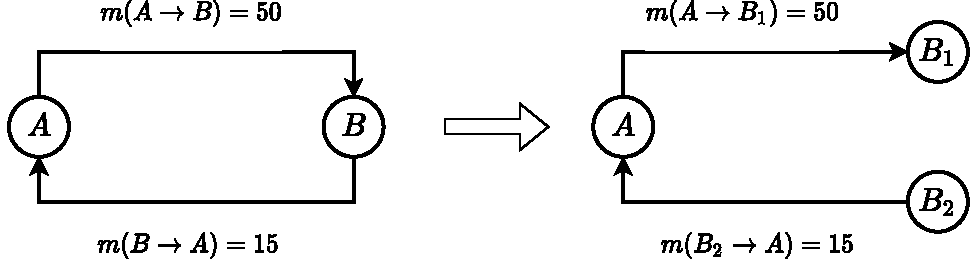
\includegraphics[width=1\linewidth]{c6/cycle-removal.pdf}
    \caption{An example of Cyclic Dependency removal. Based on Lippert's example \cite[p. 128]{Lippert2006}.}
    \label{c6:fig:cd-removal}
\end{figure}

As an example to better understand the reasoning behind this approach, let us take into consideration the case of a CD smell instance between two classes A and B (see Figure \ref{c6:fig:cd-removal}). In order to remove it, the traditional way \cite[p. 128]{Lippert2006} is to split B in two (or more) segments $B_1$ and $B_2$ and separate dependencies in such a way that A depends on $B_1$ (or $A \rightarrow B_1$), and $B_2$ depends on A (or $B_2 \rightarrow A$).
This process implies that the developer must be familiar with all dependencies between A and B. For the sake of the example, let us assume that each line of code contains one dependency only. Then, we calculate, we count all the lines of code in A that use or create the dependency $A \rightarrow B$, and those for $B \rightarrow A$. Then we have $m(x) = m(A \rightarrow B) + m(B \rightarrow A) = 50 + 15 = 65$ LOC, which is the number of lines of code one needs to understand before deciding on how to split B and proceed with the refactoring. In Figure \ref{c6:fig:cd-removal}, only $m(B \rightarrow A) = 15$ LOC were eventually moved to a new class, but the whole 65 lines of code were needed be understood before refactoring the 15 creating the dependency $B \rightarrow A$.

An architectural smell is comprised of several artefacts. Each artefact has a series of dependencies towards other artefacts, which we consider as edges (i.e. $A \rightarrow B$). We calculate 
\begin{equation}\label{c6:eq:smell-extent-dependency}
    m(x) = \sum^{E_x} w(a \rightarrow b)
\end{equation}
where $$E_x = \{a \rightarrow b | a,b\textnormal{ are classes or packages affected by smell } x\}$$ and $w(a\rightarrow b)$ calculates the number of times artefact $a$ uses artefact $b$. 
By use we mean any time $a$ declares a variable of type $b$, invokes a method on an object of type $b$, accesses a field of an object of type $b$, or inherits from type $b$.
The way we calculate dependencies complies with the benchmark and guidelines provided by Pruijt et al. \cite{Pruijt2017}.

One can also see the $m$ function as a special, finer-grained case of the dependency edge weight function defined by Laval et al. \cite{Laval2012}, where instead of counting the import statements only, we count all the lines of code directly using such dependency.

An advantage of $m(x)$ is that it allows to handle the overlap between smells at a fine-grained level and avoid overestimation of the final effort calculated to remove all the smells (i.e. a single edge may be responsible for the creation of multiple smells). 
This is simply achieved using the following generalisation of Equation \ref{c6:eq:smell-extent-dependency}:
\begin{equation}\label{c6:eq:smell-extent-dependency-weight}
m(x) = \sum^{E_x} \frac{w(a\rightarrow b)}{o(a \rightarrow b)}
\end{equation}
where the contribution of each edge $a \rightarrow b$ is weighted by the number of smells that edge contributes creating, calculated by $o(a \rightarrow b)$.

Another advantage is that it allows to identify which edges yield the highest return on effort invested if removed, because one can target the edge with lowest use and highest number of smells passing through it.
Additionally, it allows to only include the edges that actually create the smell, for example, for UD smell, $m(x)$ may only include the edges that create dependencies towards less stable packages.

In \textsc{Arcan}, this feature is implemented by relying on Spoon \cite{Pawlak2015} to precisely calculate the lines of code generating a dependency (as defined by Pruijt et al. \cite{Pruijt2017}).

\paragraph{Size-based smells}
God Component is a smell that is detected based on the number of lines of code an artefact has (calculated summing up the LOC of the \emph{directly} contained files) and whether it exceeds a certain threshold.
The threshold is calculated using an adaptive statistical approach that takes into consideration  the number of LOC of the other packages in the system and in a benchmark of over 100 systems \cite{Arcelli2015}.
The adaptive threshold is defined in such a way that it is always larger than the median lines of code of the packages/components in the system and benchmark.
Therefore, the goal of refactoring a God Component is to reduce the total number of lines of code in the system to be in line with the rest of the components in the system (i.e. get closer to the median of the system).
As mentioned earlier, the lines of code metric is a known predictor of complexity \cite{Lippert2006, Morasca2001, Kitchenham2004}, therefore to formalise this concept we define 
\begin{equation}\label{c6:eq:smell-extent-gc-threshold}
    \delta(x) = LOC(x) - T_{median}   
\end{equation}
where $LOC(x)$ calculates the lines of code of in the artefact affected by the smell $x$, and $T_{median}$ is the median size of components in the system.

However, just the bare number of lines of code is not fully indicative of the effort.
The number of elements and the connection among those elements is a variable affecting the difficulty of performing such task. The more elements (and connections among them) there are in a component, the lower its Understandability \cite[p. 32]{Lippert2006} and the higher their coupling.
Therefore, we define the extent of a god component architectural smell as
\begin{equation}\label{c6:eq:smell-extent-gc}
    m(x) = \delta(x) \cdot \sqrt{\frac{|E_x|}{2|V_x|}}
\end{equation}
where $|E_x| \ge 1$ and $|V_x| \ge 1$ are the number of edges and vertices respectively, contained in the subgraph created within the artefact affected by $x$.
The second term in Equation \ref{c6:eq:smell-extent-gc} ensures that if there is loose coupling among the elements contained in the component affected by $x$, then the overall value is lower, because it is easier to identify what files to move to another component, or what files to split into multiple files before moving them. The square root is used to reduce the effect on the final result.
Indeed, early experimentation without the use of the second term resulted in over-estimations of the index in cases were the internal elements of a package were loosely coupled.

\subsubsection{Summary definition}
The $m$ function has a different definition based on the type of smell evaluated. To avoid misunderstandings, we formalise this in the present section by defining $m$ as follows:
\begin{equation}\label{c6:eq:smell-extent-all}
    m(x) = \begin{cases}
        \sum^{E_x} \frac{w(a\rightarrow b)}{o(a \rightarrow b)} & \text{if $x$ is a CD, HL, or UD instance}\\
        \delta(x) \cdot \sqrt{\frac{|E_x|}{2|V_x|}} & \text{if $x$ is a GC instance}\\
    \end{cases} 
\end{equation}
where $x$ is an architectural smell instance, and the rest of the variables and functions are the same as defined in the previous sections.


\section{Case study design}\label{c6:sec:study-design}
To evaluate the approach described in Section \ref{c6:sec:approach}, we followed the guidelines proposed by Runeson et al. \cite{Runeson2012} to design an holistic multiple-case study.
Case studies are commonly used in software engineering research to study a phenomenon in its real-life context \cite{Runeson2012}.
We opted to perform a case study because it allows us to investigate the practical application of our approach in the context of both industrial and open source projects. 
In the next sections we elaborate on the study design.

%We list the threats to the validity of this case study and the actions undertaken to mitigate them in Section \ref{c6:sec:threats-to-validity}.

\subsection{Goal and research questions}\label{c6:sec:goal-and-rqs}
The objective of the case study is to evaluate the \emph{accuracy}, \emph{transparency}, and \emph{relevance} of our approach that estimates architectural technical debt principal using architectural smells.
Using the Goal-Question-Metric \cite{VanSolingen2002} formulation, the objective is stated as follows:
\begin{quote}
    \itshape
    \textbf{Analyse} the approach estimating architectural technical debt principal \textbf{for the purpose of} validating its application \textbf{with respect to} accuracy, transparency, and relevance of the estimation output \textbf{from the point of view of} software developers \textbf{in the context of} open source and industrial software systems.
\end{quote}
The goal can be further refined into the following two research questions, reflecting accuracy and relevance respectively:
\begin{itemize}
    \item[\textbf{RQ1}] Can the approach rank architectural smells by their severity?
    \begin{itemize}
        \item[\textbf{RQ1.1}] How accurate is the ranking of AS by different ML models?
        \item[\textbf{RQ1.2}] How do smell characteristics impact the predictions of severity?
    \end{itemize}
\end{itemize}
Essentially, we are interested in the accuracy and transparency of the output of the approach, i.e. the principal. Our approach uses two factors to estimate the principal of each smell instance: severity and extent. We do not need to validate the accuracy and transparency of the smell extent, as that can be measured directly on the source code generating the smell. 
Thus, RQ1.1 concerns the \emph{accuracy} of calculating smell severity, and particularly the accuracy of the machine learning model in ranking architectural smells by their severity.
We will assess the accuracy of the model using an evaluation metric specific to ranking tasks as described in Section \ref{c6:sec:perf-metric}.
RQ1.2 focuses on measuring the \emph{transparency} of the machine learning model. Namely, it will explain how the model effectively makes predictions on new, unseen instances, thus allowing us to better understand which smell characteristics make a smell more severe than another.
This will also ensure that the model is not using undesired variables to predict the severity of a specific smell (e.g. the Shape characteristic is only used for CD instances, and should be be used to predict the severity of a HL).

\begin{itemize}
    \item[\textbf{RQ2}] Is the principal estimated by the approach relevant to software developers?    
    \begin{itemize}
        \item[\textbf{RQ2.1}] Does the estimated principal represent the effort necessary to refactor an architectural smell?
        \item[\textbf{RQ2.2}] Are the size and order of the estimations of individual smells meaningful in relation to each other? 
        \item[\textbf{RQ2.3}] What do software developers think about the proposed approach overall?
    \end{itemize} 
\end{itemize}
This research question assesses if the whole approach is relevant, in terms of providing an actionable output to developers (i.e. can they make decisions using the output provided by the approach?).
We answer this research question by answering the three sub-questions.
RQ2.1 focuses on how far the estimated principal correlates with the effort expected by the engineers to refactor a certain instance. 
This would allow engineers to \emph{reliably plan} the allocation of their resources (e.g. time) during the repayment phase.
RQ2.2 focuses on whether the approach allows comparisons between different smell instances (e.g. if this smell's estimated ATDI is $x$ than it makes sense for the other smell's ATDI to be $y$).
If indeed the magnitude and relative size of the estimations with respect to each other are meaningful, then the approach provides the means to make \emph{evidence-based} prioritisation decisions for resolving smells.
Finally, RQ2.3 aims at understanding the \emph{general opinion} of software developers towards architectural smell analysis and the estimations provided by ATDI.

\subsection{Detailed overview of the case study}
The two research questions (RQ1 and RQ2) correspond, respectively, to two different phases of this study: \textbf{model engineering \& verification} and \textbf{model validation}.
Figure \ref{c6:fig:study-overview} depicts a detailed overview of these two phases, while Section \ref{c6:sec:rq1-methodology} and Section \ref{c6:sec:rq2-methodology} respectively describe the two phases in detail.

A replication package of this study is available online\footnote{Visit \url{https://dx.doi.org/10.6084/m9.figshare.19823323} to access it.} and contains all the material used to design this case study.

\begin{figure*}
    \centering
    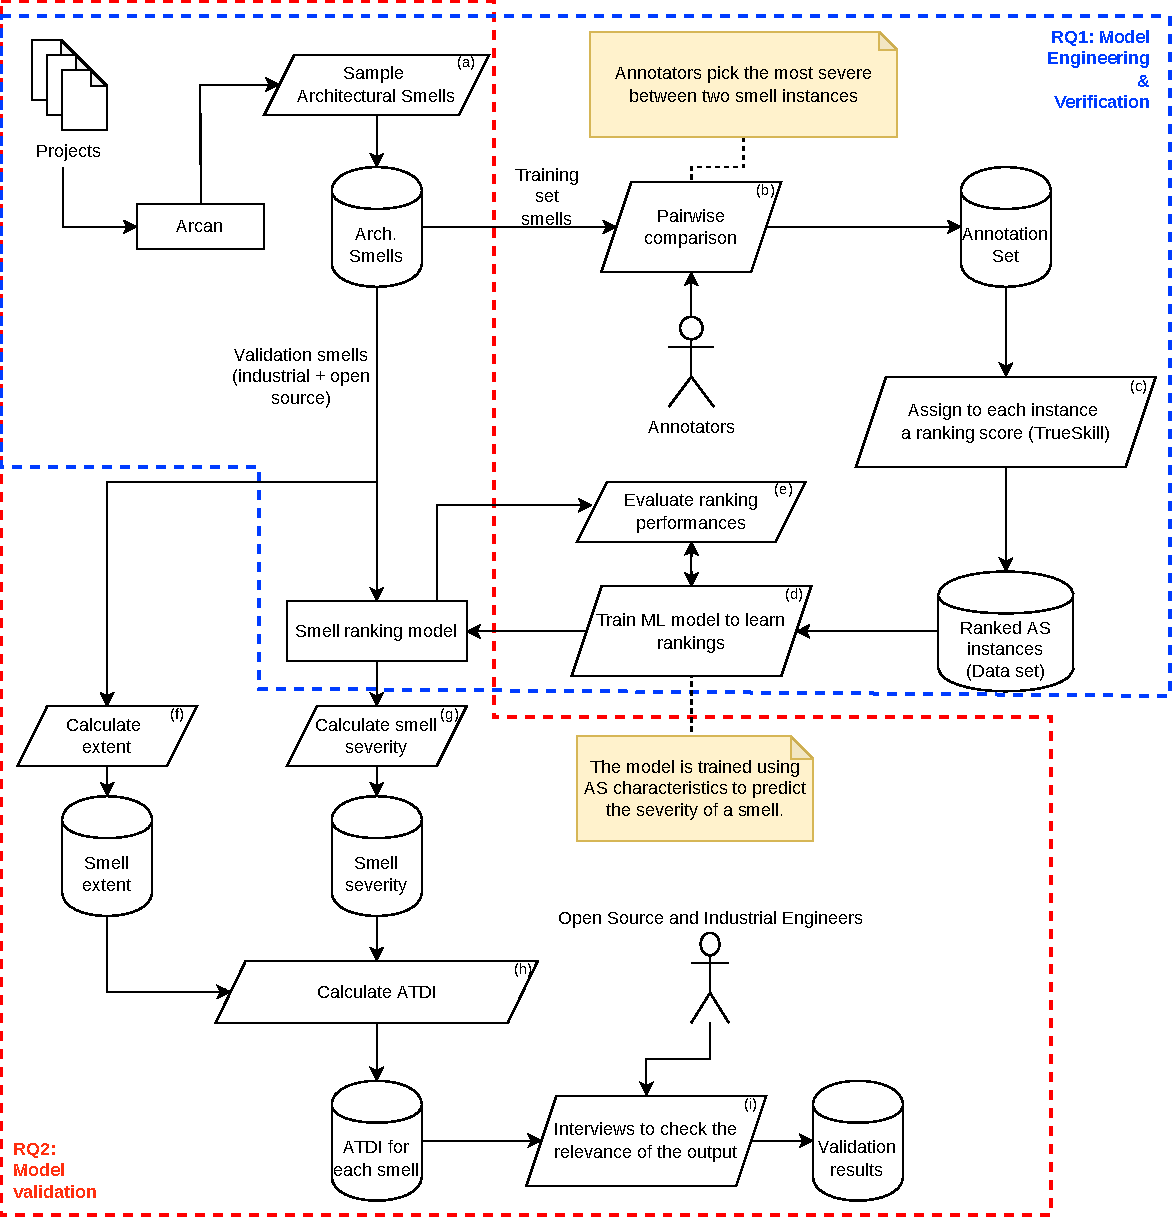
\includegraphics[width=\textwidth]{c6/learn-to-rank.pdf}
    \caption{Detailed diagram of the model engineering and model evaluation phases.}\label{c6:fig:study-overview}
\end{figure*}

\subsection{RQ1: Model engineering \& verification}\label{c6:sec:rq1-methodology}
\subsubsection{Dataset creation}
\paragraph{Sampling the smells}
To answer RQ1 we trained a machine learning model to rank architectural smells by their severity.
The first step necessary to do so, as shown in Figure \ref{c6:fig:study-overview}, step \emph{(a)} was to collect the data necessary to train the machine learning model, i.e. the architectural smells. This entailed choosing a set of projects to mine the smells from using \textsc{Arcan} (see Section \ref{c6:sec:AS}). 
The selection criteria to choose the projects were the following:
\begin{enumerate}
    \item The projects must have more than 10.000 LOC; 
    \item The projects must have at least one instance of each architectural smell type;
    \item The annotators must be familiar with the architecture of the system they are annotating.
\end{enumerate}
These criteria ensured respectively that: 1) the projects selected were sufficiently big to contain enough architectural smells; 2) for each project there can be a comparison between all smell types; 3) the annotated smells affected parts of code that the annotators were familiar with, thus being able to provide a relevant annotation.
The projects selected by this process are shown in Table \ref{c6:tab:smells-data-set}, along with the number of smells sampled from each project.
Smells were sampled using stratified sampling based on their type and project.
Namely, we tried to import as many smells as possible of the less frequent types (i.e. GC) while also preventing to bias our data set by sampling too many smells from the larger projects (e.g Spoon and JMeter).

\begin{table}[]
    \footnotesize
    \centering
    \caption{The projects used for sampling smells and the number of smells compared as well as the number of comparisons.}
    \label{c6:tab:smells-data-set}
    \begin{tabular}{@{}lccc@{}}
    \toprule
    \textbf{Project} & \textbf{\#Smells sampled} & \textbf{\#Smells compared} & \textbf{\#Comparisons} \\ \midrule
    Arcan & 55 & 14 & 23 \\
    AStracker & 28 & 7 & 7 \\
    Emma & 54 & 10 & 15 \\
    JMeter & 154 & 22 & 77 \\
    JUunit4 & 29 & 7 & 7 \\
    Spoon & 155 & 22 & 77 \\
    Spring-boot & 92 & 15 & 35 \\
    Struts2 & 84 & 14 & 30 \\ \midrule
    \textbf{Total} & \textbf{651} & \textbf{111} & \textbf{271} \\ \bottomrule
    \end{tabular}
\end{table}

\paragraph{Annotation set creation}
The smells sampled from the selected projects were then used to create an annotation set that contained, for each record, a pair of smells and an annotation denoting which one of them is the most severe one.
As one can see in Figure \ref{c6:fig:study-overview}, step \emph{(b)}, annotations were manually created using \emph{pairwise comparison}, a process for annotating entities \cite{David1963} where an annotator is asked to compare two entities w.r.t. a certain quantitative property and provide a qualitative judgement on which one of the two entities is best.
The main reason for using pairwise comparisons over rating scales (e.g. Likert scale) is that it avoids several problems typical of rating scales. 
More specifically, rating scales are relative, which means that a value of 4 may not represent a similar quantity for two different individuals.
Also, the quantity represented for one individual may change during the questionnaire (e.g. after answering more questions) or if repeated in different days \cite{Perezortiz2017}, whereas, if two smells are compared twice and obtain discordant ratings, their final ranking will just depend more on the annotations where the two smells were compared with other smells.
These disadvantages make a rating scale, such as a Likert scale, a poor choice for this step.

The main drawback of pairwise comparison is the very large amount of comparisons necessary to achieve an order among the elements compared.
Pairwise comparisons necessitates $\binom{n}{2}$ comparisons. If we want to create a data set with $n = 500$ elements, then \emph{124.750} comparisons are necessary.
This number is infeasible for the purposes of our study; therefore, we adopted an array of techniques to reduce this number while at the same time increasing the number of elements in our data set:
\begin{enumerate}
    
    \item \emph{Active Sampling} is a technique that chooses the pairs to compare based on which one gives the most amount of information \cite{Mikhailiuk2020}. This technique is basically a compromise between number of comparisons and accuracy of the ranking with respect to the ground truth (i.e. the order obtained by doing $\binom{n}{2}$ comparisons). 
    The more comparisons are performed, the lower the error accumulated.
    Moreover, active sampling allows to reduce this error much faster than random selection of pairs to compare. 
    Several state-of-the-art techniques exist to perform this task, but ASAP \cite{Mikhailiuk2020} is the latest and fastest at the moment of writing.
    With this technique, we are guaranteed to reach at worse a 15\% error within $\frac{1}{3}\binom{n}{2}$ comparisons.
    
    This technique alone, however, is not sufficient to reduce the number of comparisons to a feasible amount.

    \item \emph{Initial ranking} gives an initial estimation of the final rank of the smell based on the architectural smells characteristics of each instance (i.e. the number of elements affected, number of dependencies, etc.). 
    The calculation of the initial ranking is based on previous work on architectural smell ranking \cite{Laval2012} and on smell characteristics \cite{Sas2019}.
    
    This allows to avoid comparisons of smells that are clearly at the two ends of the ranking range (e.g. a cycle of size 20 and a cycle of size 3).

    \item \emph{Neighbourhood Representative Sampling (NRS)} is based on the core concept behind the $k$-nearest neighbours ($k$-NN) algorithm, a classification and regression model widely used in machine learning \cite{Fix1989}: \emph{similar instances will probably have a similar classification}.
    This rationale can also be applied to the initial ranking, namely, \emph{similar instances will have a similar initial ranking}.
    Therefore, if we choose $k$ as the number of neighbourhoods and `appoint' one representative for each neighbourhood, we only have to compare $k$ elements rather than $n$.
    Obviously, the smaller the value of $k$, the more precise the final ranking.
    We selected $k$ with the following formula $k = \lfloor\log_2 n\rfloor$ for all $n \ge 5$, otherwise we used $k = 1$ (i.e. compared all smells).

    \item \emph{Intra-project comparisons} entails comparing smells from the same project only. It is justified because comparing two smells from two different projects is not intuitive and there are no common points that an annotator can use to make a proper comparison.
    For example, the depth in the package containment tree (PCT) of the affected elements, a well-known smell characteristics used for ranking \cite{Laval2012}, would be hard to apply by a human as different projects have different PCT structures.

\end{enumerate}
These four techniques are combined as follows: we first assign an initial ranking to each smell; then, we choose $k$ neighbourhoods and pick a smell that has the most similar initial ranking in that neighbourhood and designate it as its \emph{representative}; next, we perform pairwise comparisons among the representatives using active sampling until we obtain an order among the representatives; finally, the ranking is extended to the other smells in the neighbourhood.
This whole process is contained in Figure \ref{c6:fig:study-overview} under the step \emph{(b)}, for the sake of simplicity.

The next question is how to go from triplets in the form of $\langle smell_1, smell_2, annotation \rangle$ (i.e. the output of the comparison process in step \emph{(b)}) to a ranked order among the elements compared -- which brings us to step \emph{(c)}.
There exist several algorithms that perform this task, but we opted for one of the most common solutions both in industry and academia, namely TrueSkill \cite{Herbrich2006}.
TrueSkill has been used extensively in information retrieval, learning-to-rank models, and even in software engineering to decide on how to assign tasks to components in simulation systems \cite{Wienss2013}, or to study the biases present in case studies analysing the language adoption of software developers \cite{Meyerovich2012}.
The TrueSkill algorithm seems the most pertinent for our purposes given its application in other software engineering research studies, as well as the wide availability of its implementation.

\paragraph{Data set creation and annotators agreement}
After completing step \emph{(c)} from Figure \ref{c6:fig:study-overview}, we obtained a data set of 651 smell instances (see Table \ref{c6:tab:smells-data-set}) that were ranked according to their severity, requiring 271 comparisons.
Comparisons required around 5 minutes each, and the whole process took 22 hours split among 3 annotators.
The annotation team was comprised of two Ph.D. students (including the first author) and a research assistant.
Inter-annotator agreement was measured using Fleiss's Kappa \cite{Fleiss1971}, obtaining a $.88$ score (considered `almost perfect agreement' \cite{Fleiss1971}).
Three test run rounds were necessary to achieve a score greater than $.8$ (i.e. greater than `moderate agreement' \cite{Fleiss1971}). 
We ensured all three annotators used the same decision-making process to annotate the data by devising a set of rules, available in the replication package \footnote{Visit \url{https://dx.doi.org/10.6084/m9.figshare.19823323} to access it.} along with the resulting annotations.
Those rules were based on the available literature \cite{Laval2012,AlMutawa2014}, our own experience on the subject, and the feedback during the three test rounds.

The distribution of the labels obtained through this process is depicted in Figure \ref{c6:fig:dataset-label-distr}.
As it can be noted, CD smells are distributed almost perfectly across the domain of severity, whereas the other smells are skewed towards higher values.
This is because CD smells are much more easily detectable and there exist many more instances that pose little threat to the maintainability of a system \cite{AlMutawa2014,Laval2012}.
This is, in contrast, rather unlikely for a GC or HL instance.
The distribution of the number of different types of smells is representative of the typical distribution found when analysing other software systems \cite{Sas2021}.

The training of the machine learning model was done using a 7-fold cross validation (step \emph{(d)}) and we evaluated ranking performance using normalised discounted cumulative gain (step \emph{(e)}).
This step (step \emph{(e)}) allows us to measure the accuracy of the ML model, i.e. to answer RQ1.
Further details on the training and performance obtained are reported in the next section.

\begin{figure}
    \centering
    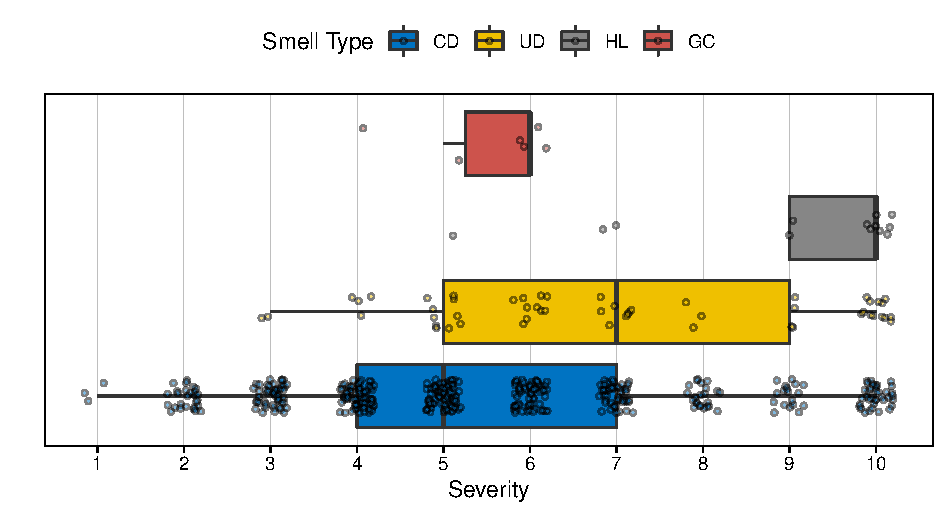
\includegraphics[width=\linewidth]{c6/dataset-label-distr.pdf}
    \caption{Distribution of (severity) labels obtained through our annotation process. Original data points are showed with slight jitter for better visualisation. Severity was rounded to 0 decimals in order to comply with LightGBM requirements.}\label{c6:fig:dataset-label-distr}
\end{figure}

\subsubsection{Training strategy \& evaluation metric}\label{c6:sec:perf-metric}
To select the most suitable model for our task, we relied on the current state-of-the-art library for LTR tasks: LightGBM \cite{Ke2017}.
The training process used is $k$-fold cross-validation \cite{Stone1974}, a process where the data set is divided into $k$ equal partitions with one partition that acts as test set and the rest as training set; the process is then repeated until all $k$ partitions acted as test set.
The main advantage of using cross-validation over classic approaches such as plain train/test partitioning is the reduction of \emph{selection bias}, ensuring that the model performs similarly regardless of the seed used to partition the data set.

The metric that is most suitable to evaluate the performance of our model is Normalised Discounted Cumulative Gain ($NDCG$) \cite{Jarvelin2002}. 
$NDCG$ is the most common metric used in information retrieval to evaluate the efficiency of an algorithm to retrieve results in a certain order \cite{Wang2018}.
As an example of its use in software engineering studies, it was used to evaluate the relevance of algorithms retrieving architectural knowledge from StackOverflow \cite{Soliman2018}.

The goal of our task is to \textit{\textbf{minimise the number of times a severe smell is ranked below a less severe smell}}.
$NDCG$ matches perfectly our goal, as it penalises smells appearing lower than less severe smells in a ranked result list.

The formula of NDCG is as follows
$$NDCG = \frac{DCG}{IDCG} = \frac{1}{IDCG}\sum_{i=1}^n\frac{\ell_i}{\log_2(i+1)}$$
where $\ell_i$ is the severity label of the smell at position $i$, $DCG$ is the discounted cumulative gain, and $IDCG$ is the $DCG$ calculated on the sequence of retrieved elements in the ideal order (i.e. we sort results by $\ell_i$ such that smells with higher values of $\ell_i$ appear first).

The $NDCG$ metric (unlike $DCG$) is defined in the interval $[0, 1]$, with higher values meaning better performance/ranking of results.
In most scenarios, $NDCG$ is calculated only for the first $n$ elements of the test set, denoted as $NDCG@n$.
By combining multiple measures of $NDCG@n$ for different values of $n$, one can gauge the performance on incremental sub-lists of the result.
In other words, $n$ restricts the focus on the performance obtained by classifying the top $n$ most severe smells in the test set.

\subsection{RQ2: Model validation}\label{c6:sec:rq2-methodology}
Figure \ref{c6:fig:study-overview} depicts the process used for the validation of the model (red frame).
In particular, we detect architectural smells in open source and industrial systems, use the machine learning model developed in RQ1, calculate $ATDI$ through calculating extent and severity, and then collect the opinions of software practitioners about the output. 
The opinions are solicited through interviews, which, as a direct data collection technique, allows researchers to control exactly what data is collected, how it is collected, and in what form it is collected \cite{Runeson2012,Lethbridge2005}. 

\subsubsection{Cases, subjects and units of analysis}
The cases of our study are the projects analysed whereas the context is either open source or industry; Figure \ref{c6:fig:case-study-design-rq2} illustrates as an example, two cases from each context, from a total of sixteen cases. 
Finally, the units of analysis correspond to the software practitioners interviewed. Since each case contains a single unit of analysis, the design of the case study is multiple and holistic (see Runeson et al. \cite{Runeson2012}).

\begin{figure}
    \centering
    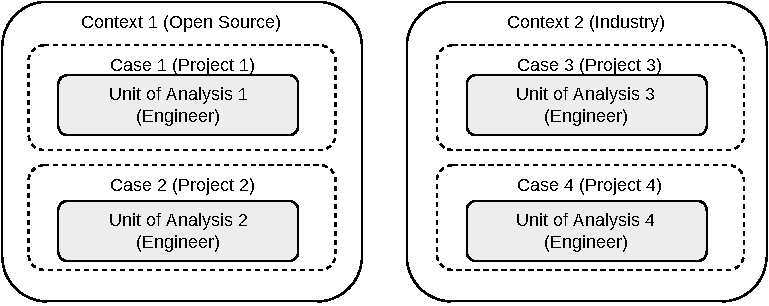
\includegraphics[width=.8\linewidth]{c6/case-study-design-rq2.pdf}
    \caption{Mapping of cases and units of analysis for RQ2; based on Figure 3.1 by Runeson et al. \cite{Runeson2012}.}\label{c6:fig:case-study-design-rq2}
\end{figure}

Tables \ref{c6:tab:open-source-participants} and \ref{c6:tab:industrial-participants} list the participants of the interviews, alongside their respective background information; the sample contains 9 engineers from open source projects and 7 from industrial projects.
We opted to interview one engineer per project (both for Open Source and  industrial projects) in order to maximise the variance of information obtained and avoid overlaps, thus extending external validity.
Note that most of the participants from open source projects are also employed in industry.

The open source participants were selected through the following process:
\begin{enumerate}
    \item We first collected a list of open source projects featured in other recent studies on Technical Debt that involved interviews and/or surveys \cite{Tan2021,Maldonado2017,Zampetti2021}. This ensured that the candidate projects contained technical debt and resulted in selecting 21 open source projects (listed in Figure \ref{c6:fig:atdi-distribution});
    \item We listed the most active contributors from the repositories of such projects (top 10\% of number of commits in the last year). We selected the most active contributors to ensure that they had deep understanding of the system (or of a specific part of it) and that they were up-to-date with the latest code. 
    This resulted in over 260 contacts, and after removing bots and invalid emails we ended up with 230 contacts;
    \item We sent out 230 invitation emails and received 37 responses, of which 11 of them contained a positive response and eventually 9 resulted in an interview.
\end{enumerate}

To select the industrial participants, we used purposeful sampling \cite{Palinkas2015}. Specifically, we got in touch with two companies from our professional network and asked them whether they were willing to participate in the study. 
The two companies are both small and medium-sized enterprises\footnote{See \url{https://ec.europa.eu/growth/smes/sme-definition_en}.} that operate in the IoT and Enterprise Application domains, respectively.
Next, we asked them to provide us with (1) a list of Java projects that had at least 10.000 lines of code, and (2) a list of engineers working on these projects that were willing to take part in the interviews.

Overall, the sample is comprised of 16 engineers (and their respective projects), characterised by a wide variety in total number of years of experience and technological background (e.g. distributed systems, testing, security, etc.).
Of course, no sample is perfect, and we elaborate on the threats to external validity entailed by the composition of our sample in Section \ref{c6:sec:threats-to-validity}.

\begin{table}[]
    \centering
    \footnotesize
    \caption{List of participants from the open source projects. Note that the `Role in project' column was \textbf{shuffled} to protect the anonymity of the participants. For example, P1 is not an idependent contractor, but one of the other participants is. Abbreviations: \textbf{Partic.}: participant; \textbf{OS}: open source; \textbf{IN}: industry; \textbf{Exp.}: experience; \textbf{PMC}: Project Management Committee; \textbf{MC}: Main Contributor.}
    \label{c6:tab:open-source-participants}
    \begin{tabular}{@{}clm{2cm}l@{}}
    \toprule
    \textbf{Partic.} & \textbf{Project} & \textbf{Exp. in} \textbf{OS/IN (Years)} & \textbf{Role in project} \\ \midrule
    P1 & Hadoop & 12 / 8 & \multirow{9}{*}{\begin{tabular}[c]{@{}l@{}}Independent Contractor\\ Team lead and MC\\ PMC member \& Contributor \\ Security Engineer \\ PMC member \\ PMC member \& contributor\\ Lead maintainer\\ Contributor\\ Project lead and MC\end{tabular}} \\
    P2 & DBeaver & 5 / 18 &  \\
    P3 & JUnit5 & 12 / 14 &  \\
    P4 & RxJava & 10 / 15 &  \\
    P5 & Jenkins & 18 / 11 &  \\
    P6 & Hibernate & 20 / 20 &  \\
    P7 & Cassandra & 8 / 24 &  \\
    P8 & Camel & 18 / 20 &  \\ %o9
    P9 & HBase & 16 / 20 &  \\ %o10 
    \midrule
    \multicolumn{2}{r}{Average} & 13.1 / 16.6 &  \\ \bottomrule
    \end{tabular}
\end{table}

\begin{table}[]
    \centering
    \footnotesize
    \caption{List of participants from the industrial projects. Abbreviations: \textbf{mgmnt.}: management; \textbf{Partic.}: participant; \textbf{Exp.}: experience.}
    \label{c6:tab:industrial-participants}
    \begin{tabular}{@{}ccm{2cm}m{0.5cm}l@{}}
    \toprule
    \textbf{Partic.} & \textbf{Company} & \textbf{Project} & \textbf{Exp. (Years)} & \multicolumn{1}{c}{\textbf{Role}} \\ \midrule
    P10 & C1 & IoT Framework & 3 & Developer \\ % o11
    P11 & C1 & Document mgmnt. system & 15 & Senior developer \\ % o12
    P12 & C2 & Project mgmnt. tool & 22 & Product manager\\ % o13
    P13 & C2 & Rent mgmnt. API service & 8 & Senior developer \\ % o14
    P14 & C2 & Parking occupancy meter & 6 & Full-Stack developer \\ % o15
    P15 & C2 & Financial assets mgmnt. & 6 & Senior developer \\ % o16
    P16 & C2 & Subscription mgmnt. & 3 & Developer \\ \midrule % o17
    \multicolumn{3}{r}{Average} & 9 &  \\ \bottomrule
    \end{tabular}
\end{table}

\subsubsection{Data collection}
Interviews were held following the guidelines mentioned by Runeson et al. \cite{Runeson2012}.
The interviews lasted 30-35 minutes and were semi-structured in their format, meaning that the interviewer could deviate from the original list of questions if a certain answer given by the participant was interesting to explore in more depth. The replication package contains the interview invitation and the questionnaire with the list of questions \footnote{Visit \url{https://dx.doi.org/10.6084/m9.figshare.19823323} to access it.}.
Each interview invitation contained (1) a one-pager with the definitions of the smell types discussed in the interviews; and (2) a letter informing the participant of the confidentiality of the interview as well as their right to not answer any question they do not wish to answer \cite{Runeson2012}.
Before the interview started, both aforementioned points were reiterated to the participants to ensure that they were familiar with the technical concepts discussed during the interview and that they agreed with the terms of the interview.
 
During the interviews, we showed the participants one instance of each architectural smell type. If one type was not detected in the particular system, we replaced it with an instance of a type already included, so as to ensure we collect the same amount of data from every engineer. 
Smells were chosen from parts of the system that the participants indicated to be most familiar with.
The smells were visualised graphically as a network where nodes corresponded to classes and packages, and edges corresponded to the dependencies among them.
Each smell was accompanied by a number representing the effort necessary to refactor that smell (i.e. the ATDI).
Next, each participant was asked whether they agree with the information presented for each instance while also keeping in mind the estimations provided for the other instances.
This ensured that their answers were consistent among different smell instances.
Finally, each participant was asked to explain their answer and particularly their rationale.
This process allowed us to minimise the amount of explanation provided to the participants (reducing the risk of confusion and bias).

Overall, the data collected for each participant are the following: (1) background information regarding their expertise; (2) whether they find the estimated principal to be representative of the required refactoring effort (RQ2.1); (3) whether they think the \emph{order and proportions} of the principal estimations were consistent among the instances presented (RQ2.2); (4) the rationale behind their answers on points (2) and (3);  and (5) their feedback on the whole analysis (RQ2.3).


\subsubsection{Data analysis}
To analyse the data collected through the interviews, we adopted the Constant Comparative Method (CCM) \cite{Glaser2017,Boeije2002}, which is part of Grounded Theory \cite{Glaser1968}. Grounded Theory (GT) is one of the most important methods in the field of qualitative data analysis. 
It has been used extensively within both social sciences and software engineering and provides a structured approach to process and analyse the data collected from multiple sources.
GT increases the theoretical sensitivity of the researcher as the data analysis progresses and eventually allows to formulate hypotheses and theory \cite{Glaser1968}.

The CCM is an inductive data coding and categorisation process that allows a unit of data (e.g., interview transcript, observation, document) to be analysed and broken into codes based on emerging themes and concepts; these are then organised into categories that reflect an analytic understanding of the coded entities \cite{Mathison2005}.

The qualitative data analysis requires interviews to be transcribed before any of the techniques mentioned above could be applied.
Transcriptions were done as soon as batches of 2-3 interviews were completed, whereas data analysis was done iteratively.
Each iteration of the data analysis process is presented in Figure \ref{c6:fig:qualitative-analysis} and is comprised of 3 phases. During the first phase (Phase A), the collected material (i.e. the initial interview transcripts) was studied and a code map was created to organise the codes used to tag the data.
After completing this phase, the coding process started (Phase B), which also involved updating and re-organising the codes based on the new understanding of the data.
Gradually, more interviews were recorded, transcribed, and coded and notes were taken with the aid of the coded data (Phase C).
In total, three iterations of data analysis were done (i.e. three times the whole process from Figure \ref{c6:fig:qualitative-analysis}): the first for the interviews with open source engineers, the second with the industrial engineers, and the third to ensure that the codes added along the way were present in all the data.
The whole process was performed by the first author of the paper, while the second author reviewed the codes and coding schemes as they were developed to reduce the risk of biases (e.g. confirmation and information bias).
To automate the data analysis as much as possible, we relied on Atlas.ti\footnote{See \url{https://atlasti.com/}.}, a dedicated qualitative data analysis tool.

\begin{figure}
    \centering
    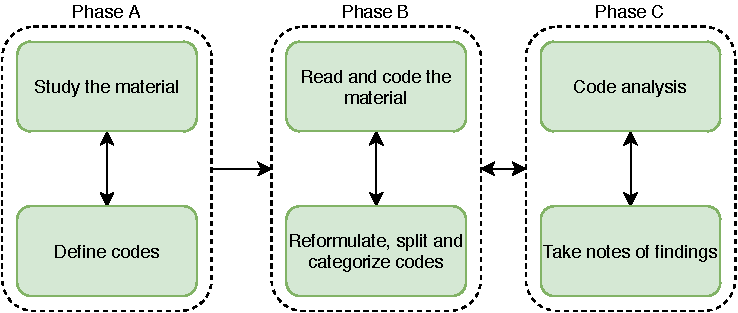
\includegraphics[width=.8\linewidth]{c6/qualitative-analysis.pdf}
    \caption{The qualitative data analysis process.}
    \label{c6:fig:qualitative-analysis}
\end{figure}

\section{Descriptive statistics of ATDI}\label{c6:sec:descriptive-statistics}
Before presenting the results of the two research questions, we briefly present some descriptive statistics about ATDI and derive some observations.
These should provide more context on the results of both RQ1 and RQ2 and allow us to understand the statistical nature of the estimations provided by the approach.

These statistics concern the same 21 projects from which we collected the names of the open source participants for RQ2 as well as the 7 industrial projects; in total, ATDI was calculated for more than 41.000 smell instances of these 28 projects.
Figure \ref{c6:fig:atdi-distribution} shows both the values of ATDI for each architectural smell instance and the value of ATDI density for the 28 projects considered.
The left-hand side plot depicts the total ATDI density for all projects, ordered from the most ATDI-dense project to the least.
The right-hand side plot depicts the distribution of ATDI for each AS instance in the 28 projects.
From the statistical analysis of the data depicted in Figure \ref{c6:fig:atdi-distribution}, we note the following:
\begin{enumerate}
    \item the highest density project is ElasticSearch with 3345.8 ATDI for each KLOC, despite being the second largest system analysed;
    \item the lowest density project is JUnit5, with 16.2 ATDI for each KLOC;
    \item an overall lower ATDI density in a project does not always imply smells with lower individual ATDI. In particular, projects with lower ATDI density than \emph{Antlr4} (i.e. below it in Figure \ref{c6:fig:atdi-distribution}), show a large variance in the ATDI of the individual instances;
    \item 50\% of AS instances have $ATDI \le 161$, and 33\% of instances have $ATDI \le 100$;
    \item there are only 37 smells with an $ATDI \ge 750$ (less than 0.001\% of all smells analysed);
    \item the maximum ATDI is 8505 by a HL smell in Jenkins;
    \item the minimum ATDI is 11, by three CDs with low severity in Camel, Cassandra and Dubbo respectively;
\end{enumerate}

\begin{figure*}
    \centering
    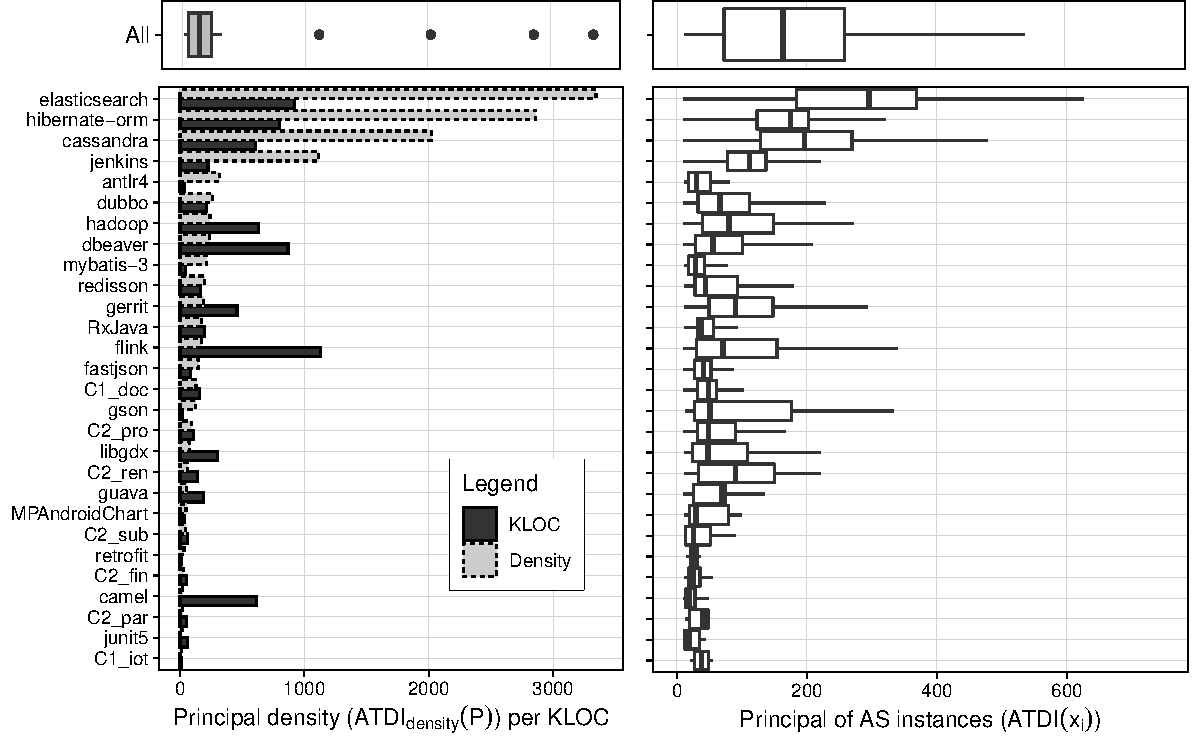
\includegraphics[width=\textwidth]{c6/principal-distribution.pdf}
    \caption{On the left, the total amount of principal (ATDI) per 1.000 lines of code (KLOC) for each project (calculated using Equation \ref{c6:eq:atdi-normalised}) compared with the number of KLOC. 
    On the right, boxplots depicting the distribution of the principal (ATDI) calculated for each AS instance (outliers not visualised). }\label{c6:fig:atdi-distribution}
\end{figure*}

% TODO
Finally, Figure \ref{c6:fig:atdi-distribution-types} depicts the distribution of ATDI for different types of AS.
There is a clear difference between the four types of AS.
GC instances are the ones with the highest ATDI principal \emph{on average}, followed by HL, CD and lastly UD.

\begin{figure}
    \centering
    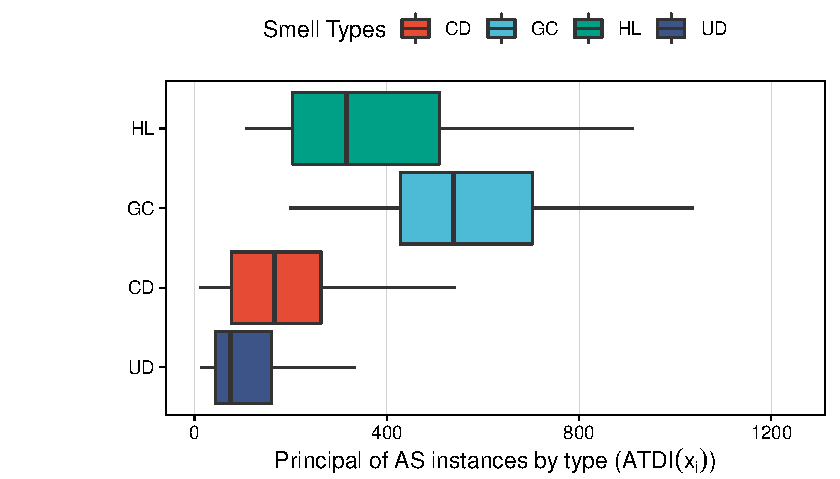
\includegraphics[width=.8\linewidth,trim=2cm 0cm 0cm 0cm]{c6/principal-distribution-type.pdf}
    \caption{Boxplots showing the distribution of ATDI for different types of AS (outliers not visualised).}\label{c6:fig:atdi-distribution-types}
\end{figure}

\section{RQ1 results}\label{c6:sec:rq1-results}
\subsection{RQ1.1: ML model accuracy}
Table \ref{c6:tab:algorithm-performances} summarises the $NDCG@n$ values obtained through cross-validation on our data set by different models.
We recall from Section \ref{c6:sec:perf-metric} that $NDCG@n$ provides higher values when the model consistently ranks severe instances above less severe ones.
Note that we opted for 7-fold cross-validation\footnote{Folds are sampled using stratified sampling on severity, which is a typical practice in Machine Learning.} over the typical 10-fold because in our case it increases the size of the test set significantly (from 65 to 93) while it also reduces overfitting (i.e. we obtain much lower variance with $k = 7$).
The results show that the best-performing algorithm is `rank\_xendcg', i.e. Cross-Entropy NDCG Loss for learning-to-rank \cite{Bruch2021}, one of the most recent and best-performing LTR algorithms.
We refer the reader to the official documentation of LightGBM for details on the other algorithms\footnote{Visit \url{https://lightgbm.readthedocs.io/en/latest/Parameters.html\#objective}.}.

Overall, `rank\_xendcg' performs very well for all values of $n$.
However, the most severe smell is not always the very first smell in the list, but it does appear very close to the top in several occasions given the score obtained for $NDCG@1 = .99$.
For values of $n > 1$, `rank\_xendcg' settles around $.90$, meaning that most instances are ranked \emph{close} to their true rank, but not all of them.
When considering the order obtained on the full size of the training sets ($n = 93$), the performance reaches $.97$.
This means that the most-severe instance is \emph{almost perfectly ranked}, the mid-severity instances are \emph{appropriately ranked} but not quite perfect, while the low-severity instances are \emph{almost perfectly ranked}.

To make these results clearer, we give four examples of smells from our data set in Figure \ref{c6:fig:severity-all}; their actual severity is obtained through the process described in Section \ref{c6:sec:rq1-methodology}, while the predicted one by the ML model.
Figure \ref{c6:fig:severity-low} depicts a CD smell with very low severity that affects one class and two of its internal classes.
Typically, this type of cycle is intentional, and given that the three classes are always expected to be reused together, this cycle does not pose any threat to maintainability, so it was labelled with the minimum severity of 1. 
The value predicted by the model was $1.84$, which is almost double the actual value, but it is still rather close.

Figure \ref{c6:fig:severity-high} shows a rather severe HL instance affecting the main \texttt{gui} package in the system\footnote{Note that there are several packages called \texttt{gui} in JMeter.} and involving 31 other packages.
Given that \texttt{gui} is aggregating a lot of functionality (when in theory it should only be responsible for the user interface) it was annotated with a severity of 10. 
The model's prediction was a bit lower at $9.11$.

Figures \ref{c6:fig:severity-medium-1} and \ref{c6:fig:severity-medium-2} depict two smells of medium severity, both are CD smells affecting 4 and 3 packages, respectively.
Both smells were labelled as medium severity of 5, because they affect packages of the system, are tightly coupled, but are not too big in number of elements affected.
The predictions provided by our model for both smells were relatively close to the actual values.

To summarise, the goal of RQ1 was to check whether a ML model can accurately rank AS by their severity. 
This is indeed the case and we were able to achieve a score of $0.97$ for $NDCG@93$, which is considered a very high score. However, there is one caveat. 
When considering the accuracy of estimating severity for  single instances  (rather than the overall rank) the model is less accurate, as shown by the examples in Figure \ref{c6:fig:severity-all}.
Namely, the model is clearly able to predict the ranking of the smells correctly, but the accuracy of the prediction is not perfect (Figure \ref*{c6:fig:severity-low}).
Nevertheless, this is both expected and acceptable, as the goal for RQ1, was to optimise for the \emph{global ranking} of instances rather than the individual prediction. Indeed, this is also what the ML model is optimising for.


\begin{table}[]
    \centering
    \caption{Performance of different algorithms for different values of $NDCG$@$n$ using 7-fold cross-validation and the standard deviation over the folds. Bold values represent the maximum in the row.}\label{c6:tab:algorithm-performances}
    \footnotesize
    \begin{tabular}{ccccm{.85cm}m{.85cm}}\toprule
    \multicolumn{1}{c}{\multirow{3}{.5cm}{$NDCG$\\@$n$}} & \multicolumn{5}{c}{\textbf{Algorithms}} \\
    \multicolumn{1}{c}{} & \textbf{mse} & \textbf{multiclass} & \textbf{multiova} & \textbf{rank\_\newline xendcg} & \textbf{lambda-rank} \\ \midrule
    1   &  .91$\pm$.00 &  .77$\pm$.04 &  .94$\pm$.01 &  \textbf{.99$\pm$.00} &  .99$\pm$.00 \\
    10  &  .87$\pm$.00 &  .86$\pm$.01 &  .88$\pm$.01 &  \textbf{.90$\pm$.00} &  .82$\pm$.00 \\
    25  &  .89$\pm$.00 &  .87$\pm$.00 &  .87$\pm$.00 &  \textbf{.90$\pm$.00} &  .87$\pm$.00 \\
    50  &  \textbf{.93$\pm$.00} &  .91$\pm$.00 &  .92$\pm$.00 &  .92$\pm$.00 &  .90$\pm$.00 \\
    93* &  .96$\pm$.00 &  .95$\pm$.00 &  .96$\pm$.00 &  \textbf{.97$\pm$.00} &  .95$\pm$.00 \\
    \bottomrule
    \end{tabular}\\
    * size of the test sets for $k=7$
\end{table}

\begin{figure}
    \centering
    \begin{subfigure}[b]{0.7\linewidth}
        \centering
        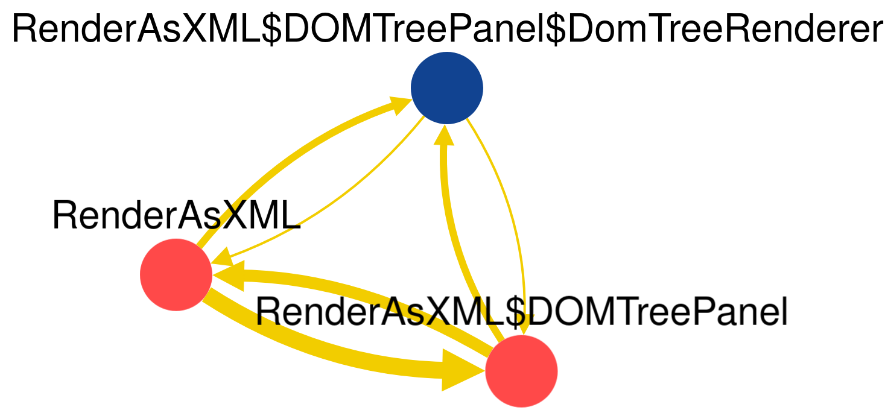
\includegraphics[width=.7\linewidth]{c6/low-severity-jmeter.png}
        \caption{CD smell; Predicted: $1.84$; Actual: $1$.}
        \label{c6:fig:severity-low}
    \end{subfigure}
    \hfill
    \begin{subfigure}[b]{.8\linewidth}
        \centering
        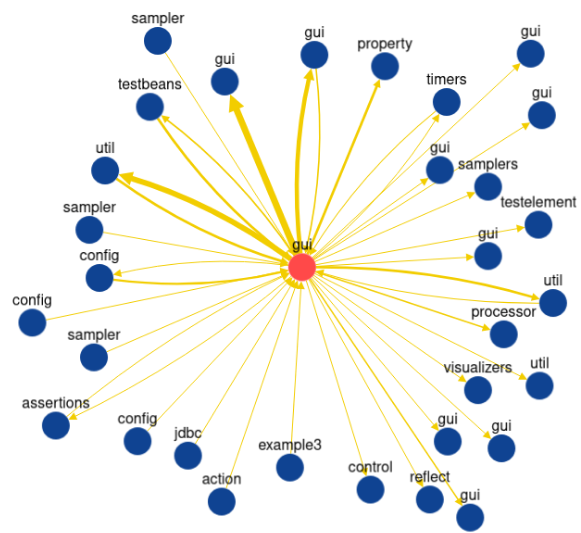
\includegraphics[width=.7\linewidth]{c6/high-severity-jmeter.png}
        \caption{HL smell; Predicted: $9.11$; Actual: $10$.}
        \label{c6:fig:severity-high}
    \end{subfigure}
    \\
    \begin{subfigure}[b]{.45\linewidth}
        \centering
        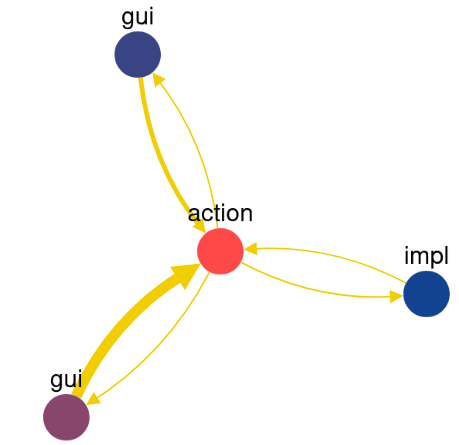
\includegraphics[width=0.7\linewidth]{c6/medium-severity-jmeter-1.png}
        \caption{CD smell; Predicted: $5.28$; Actual: $5$.}
        \label{c6:fig:severity-medium-1}
    \end{subfigure}
    \begin{subfigure}[b]{.45\linewidth}
        \centering
        \includegraphics[width=0.7\linewidth]{c6/medium-severity-jmeter-2.png}
        \caption{CD smell; Predicted: $5.46$; Actual: $5$.}
        \label{c6:fig:severity-medium-2}
    \end{subfigure}
       \caption{Example of architectural smells from our data set with their predicted and actual severity. Smells are all from the JMeter project. The width of the edges reflects the weight of the dependency, while the colour of nodes reflects the number of weighted incident edges (red means higher values; blue lower).}
       \label{c6:fig:severity-all}
\end{figure}

\subsection{RQ1.2: The contribution of smell characteristics to predictions}\label{c6:sec:explain-predictions}
Our model is able to predict quite accurately the severity of an architectural smell instance; however, it is also important to understand what smell characteristics are used, and how they impact the prediction. Namely, we want to improve the \emph{transparency} of the model by studying how it performs the predictions.
To do so, we used an approach called SHAP (SHapley Additive exPlanations). SHAP uses game theory to link the input of a model (i.e. the smell characteristics) to its output (i.e. the severity) \cite{Strumbelj2014} and explore the correlation visually.

Figure \ref{c6:fig:feat-explain-shap} depicts the importance of the smell characteristics (or features) according to the SHAP method. Values on the $x$-axis represent the output of the SHAP method: positive values entail that a feature contributed positively (i.e. increased severity) to the output of the model whereas negative values provided a negative contribution (i.e. decreased severity).
We expect the model to match the assumptions in the literature in order to establish that it works as intended.

The \emph{Size} feature (i.e. number of affected elements) contributes the most to the severity of the smell, with higher values of \emph{Size} increasing the severity and small values being neutral.
The \emph{PageRank} of the affected elements comes second, with higher values positively contributing to the severity of a smell.
This means that elements that are more central in the dependency network of the system \textbf{make a smell more severe}.
The \emph{Number of edges} feature has a similar impact as \emph{Size} (they are indeed correlated \cite{Sas2019}), but low values decrease the severity of a smell, instead of being neutral.
The metrics based on the \emph{Package Containment Tree (PCT)} \cite{Laval2012,AlMutawa2014} were relatively important too.
High values of \emph{St.dev. PCT Depth}, namely, when a smell affects both elements at the top and bottom of the PCT, positively contributes to increase the predicted severity.
Similar with the \emph{St.dev. PCT Distance}, namely, when a smell affects elements from distant branches of the PCT.
In both cases, it is interesting to note that the mean of both \emph{Distance} and \emph{Depth} are less important than their standard deviation.

After considering these results, we can confirm that the way the model uses the features reflects what is expressed in the literature.
More specifically, the smell gets more severe in cases when its size increases \cite{Lippert2006}, its \emph{centrality} in the dependency network of the system is higher \cite{Roveda2018}; also, under the assumption that distant elements in the PCT are more likely to implement different concerns \cite{Laval2012}, the smell affects elements that are  \emph{unrelated}.

\begin{figure}
    \centering
    \includegraphics[clip, trim=1.1cm 2cm -0.5cm 0cm, width=.8\linewidth]{c6/feat-explain-shap-mod.pdf}
    \caption{Importance as calculated by the SHAP method \cite{Strumbelj2014}. The higher on the $y$-axis the higher the importance.  Positive values on the $x$-axis mean that the feature contributes to increase the severity of a smell, whereas negative values do the opposite. Colour is mapped to the value assumed by the feature.} 
    \label{c6:fig:feat-explain-shap}
\end{figure}


\begin{figure*}
    \centering
    \begin{subfigure}[b]{\linewidth}
        \centering
        \includegraphics[clip, trim=0cm 2cm 0cm 0cm,width=\textwidth]{c6/explain-r124.pdf}
        \caption{Output explanation of Figure \ref{c6:fig:severity-low}.}
        \label{c6:fig:explain-low}
    \end{subfigure}\\
    \begin{subfigure}[b]{\linewidth}
        \centering
        \includegraphics[clip, trim=0cm 2cm 0cm 0cm, width=\textwidth]{c6/explain-r230.pdf}
        \caption{Output explanation of Figure \ref{c6:fig:severity-high}.}
        \label{c6:fig:explain-high}
    \end{subfigure}
    \\
    \begin{subfigure}[b]{\linewidth}
        \centering
        \includegraphics[clip, trim=0cm 2cm 0cm 0cm, width=\textwidth]{c6/explain-r178.pdf}
        \caption{Output explanation of Figure \ref{c6:fig:severity-medium-1}.}
        \label{c6:fig:explain-medium-1}
    \end{subfigure}
    \\
    \begin{subfigure}[b]{\linewidth}
        \centering
        \includegraphics[clip, trim=0cm 2cm 0cm 0cm, width=\textwidth]{c6/explain-r173.pdf}
        \caption{Output explanation of Figure \ref{c6:fig:severity-medium-2}.}
        \label{c6:fig:explain-medium-2}
    \end{subfigure}
       \caption{Prediction explanation of how severity was calculated for smells in Figure \ref{c6:fig:severity-all}. The $x$ axis represents the severity (i.e. output of the model), the blue bars represent a reduction of severity (i.e. negative contribution to prediction). Red bars represent an increase in severity (i.e. positive contribution to prediction). Each segment belongs to a specific feature only. The size of the contribution corresponds to the length of each segment and can be read on the $x$-axis. The value shown next to each feature is the normalised value the feature assumes for the smell instance (i.e. it is \emph{not} the contribution). The number in bold shown above the $x$-axis is the predicted severity for the instance.}
       \label{c6:fig:explain-all}
\end{figure*}

SHAP is also able to explain the output of single instances.
Figure \ref{c6:fig:explain-all} depicts the force plots on how smell characteristics (i.e. features) contributed to the predictions shown in Figure \ref{c6:fig:severity-all}.
For the low-severity smell, Figure \ref{c6:fig:explain-low} shows that  \emph{all features} contributed to reduce the predicted severity of the instance.
The \emph{Number of edges} and \emph{PageRank} features were the two main drivers for the decision.
An almost opposite situation can be observed in Figure \ref{c6:fig:explain-high} for the smell with the highest severity, but in this case the high number of connections (i.e. \emph{Number of edges}) and the fact that smell involves several elements from different parts of the system (i.e. high \emph{Std. dev. PCT Depth}) were the two main drivers behind the prediction of the model. 
Concerning the two smells with similar severity, we can notice in Figures \ref{c6:fig:explain-medium-1} and \ref{c6:fig:explain-medium-2} that the \emph{PCT characteristics} push for a higher severity, but the size-based characteristics push for a lower severity.
These two opposite forces result in a decision that settles towards the middle of the output scale.

In summary, by showing what AS characteristics are used by our model (and how) allows us to better understand what constitutes a severe smell and what does not.
More importantly, it increases the reliability of our study as we do not treat the ML model as a black box. 
Instead, we provide data to explain why it works well and that the identified reasons are in line with what we expected from the literature.


\section{RQ2 results}\label{c6:sec:rq2-results}
In this section we report on the results obtained by analysing the data collected through our interviews.
Note that this section concerns the estimations of the index (as defined by Equation \ref{c6:eq:atdi-smell}), which are calculated using severity (i.e. RQ1 model) but also the extent of the smell.
In the upcoming sections, we first report the opinion of the engineers on the estimations of architectural debt principal to answer RQ2.1 and RQ2.2.
Then, we report the general feedback we received from the engineers concerning our approach to answer RQ2.3.
Finally, we conclude by reporting on a few drawbacks and possible improvements of our approach.

\subsection{Perception of the ATDI estimations (RQ2.1 \& RQ2.2)}
\subsubsection{Overview}
Overall, the feedback provided by the participants regarding how well the estimated principal represents the refactoring effort (RQ2.1), was rather positive.
Of the 62 total smell instances that we discussed and their respective ATDI estimations\footnote{Note that for a few participants we did not have time to discuss all 4 instances.}, shown to the participants, 71\% (44/62) of the estimations were described as \emph{\textbf{representative}} of the effort necessary to refactor.
More specifically, responses on industrial instances showed 81\% agreement rate with the estimations provided by the index, whereas for smell instances detected in open source projects the agreement rate with the index was 65\%.
Of the 29\% (18/62) of total instances that were off the mark, only 10 of them were off by more than 100. 
The other 8 instances were off by less than 100, but since 6 of these were small instances, with an $ATDI \le 100$, the relative error was higher, so they were perceived by the participants as a big over-, or under-estimation.
Note that from our descriptive analysis of ATDI (see Figure \ref{c6:fig:atdi-distribution}), we know that only 33\% of instances have an $ATDI \le 100$, so the extent of the imprecision is limited to a small percentage of these 33\% of instances.

Concerning the magnitude and relative size of the estimations (RQ2.2), 62\% (10/17) of the participants \emph{\textbf{totally agreed}} with the relative size and order of the estimations, while 26\% (4/17) of the participants \emph{disagreed} with the ranking of a single instance only, and the remaining 12\% (2/17) with more than one.
Participants interviewed on industrial projects had a much higher rate of agreement with the ranking and relative size of the estimations than open source participants.
85\% (6/7) of industrial participants completely agreed with the ranking and relative size, whereas only 44\% (4/9) of the open source participants did so.
The rest of the open source participants (5/9) made either one or two corrections to the order.
Note that these were mostly made on instances with an $ATDI < 100$.

The aforementioned numbers provide a quantitative overview of the perception of the participants regarding the validation of ATDI.
In the next sub-section, we will give examples of six different cases, in order to provide a richer, qualitative description of both the smells and the participants perception.  
The examples were chosen to best represent the various aspects of our data set such as: (1) the ratio of agreement/disagreement with estimations; (2) whether the project is open source or industrial; (3) whether it concerned large or small smell instances; and finally, (4) whether the  cases simply presented more insights.

\subsubsection{Example opinions of the participants}\label{c6:sec:examples}
\paragraph{Example 1: \emph{RxJava}} This first example describes how two architectural smells of two different types, GC and HL, are estimated and compared by participant P4.
The GC smell was detected on the package \texttt{io.reactivex.rxjava3.core}, directly containing $52.000$ lines of code spread across 44 classes -- much higher than the average of $10.000$ lines of code circa detected in the other packages of the system.
P4 mentioned that the \texttt{core} package provides access to all the functionality of RxJava through 5 core classes, described as ``god classes''.
For this reason, P4 was exceedingly confident that the estimated value of 1500 for $ATDI$ was \textbf{justified and representative}.

The HL smell was detected on one of the 5 god classes, \texttt{io.reactivex.rxjava3. core.Flowable}, that is part of the GC smell.
This class has an overwhelming number of ingoing and outgoing dependencies, namely 264; in other words, there are 264 other classes that either depend on, or are depended by \texttt{Flowable}.
P4 mentioned that this did not cause any significant technical issue as \texttt{Flowable} does not contain any logic, but it did raise many concerns among the users of RxJava as they lamented the presence of too many methods in this class (as well as in the other 4 god classes).
For these reasons, P4 stated, with great confidence, that the estimated value of 385 for $ATDI$ was \emph{correctly} representing the effort necessary to refactor, and added that it made sense for it to be close to a fifth of the amount estimated for the GC smell as the other four classes shared the same issues and together constitute GC smell itself.

\begin{quote}
    P4: \emph{``[...] this package [the god component] contains, among others, 5 huge classes, which you could consider 5 god classes. So it makes sense to have such a big value for the index.
    There are no real technical issues with it, but users do complain about having too many methods on these god classes.''}
\end{quote}

It is worth mentioning that P4 admitted that every time a new feature was added to the system, these 5 classes were bound to change significantly, as they had to be adapted to the new functionality, as well as updated with the latest Java documentation.

\paragraph{Example 2: \emph{Occupancy of parking facilities}}
This example features a project provided by C2 that monitors occupancy in parking facilities.
The smells discussed for this system were two HL, one affecting a class and the other a package.

The HL at the package level was detected on the \texttt{service} package, the core package of the system containing all the services\footnote{Services are implemented through the Spring Framework.} provided by the system.
The package had a total of 23 ingoing and outgoing dependencies, meaning that it was connected to the majority of the packages in the system.
The estimated $ATDI$ for this smell was $600$.
The \texttt{service} package also contained an HL at class level, namely the \texttt{UserService} class, with 38 ingoing and outgoing dependencies.
This HL smell had an estimated $ATDI$ of 150.
P14 confirmed that estimations for both smells were \textbf{reasonable} as the \texttt{service} package contained the core business functionality of the system (with classes such as \texttt{UserService}), thus making it both very risky (i.e. changes may propagate easily) and very hard to change (i.e. the package is complex because of the business logic).
Moreover, P14 mentioned that \texttt{UserService} was clearly contributing to the \texttt{service} package being an HL as it depended on classes outside \texttt{service} itself, but there were also several other classes contributing to the unbalanced number of dependencies that make \texttt{service} itself a HL.

\begin{quote}
    P14: \emph{``Considering that every single business logic is in there [the \texttt{service} package], yes, I believe that it [the index] is proportionally correct. Especially with respect to the \texttt{UserService} class. The business logic of our services is the most difficult to change, whereas \texttt{UserService} class is relatively easier to change''}.
\end{quote}

\paragraph{Example 3: \emph{Document management system}}
This example features a project provided by C1 affected by several smells.
Among the four smells discussed with P11, the CD is the most interesting to look at due to the counter-intuitive nature of the smell and the estimated ATDI value.

The CD is depicted in Figure \ref{c6:fig:c1-docmgmnt-examples} (anonymised to respect the intellectual property of C1) and it affects 8 classes scattered across 6 different packages. 
The classes involved are part of the Model-View-Controller architectural pattern and their purpose is to retrieve data from the database and display it to the user in a view.
Despite these classes being rather intertwined, our model estimated an $ATDI = 65$, a rather low value for eight classes that are so much interconnected. Participant P11 agreed with the estimations, justifying them as follows:

\begin{quote}
    \emph{``The [estimated value] seems pretty good. [...] There are some dependencies that we cannot remove, and I can't see any dependencies that shouldn't be there. So all the dependencies are desired.''}.  
\end{quote}

\begin{figure}
    \centering
    \includegraphics[width=.4\linewidth]{c6/c1-docmgmnt-examples.pdf}
    \caption{A cycle among 8 classes detected in one of C1's system.}
    \label{c6:fig:c1-docmgmnt-examples}
\end{figure}

\paragraph{Example 4: \emph{Jenkins}}
The fourth example features smells detected in the Jenkins project.
Jenkins is a well-known build automation system that has a rather long and convoluted development history.
This resulted in many architectural smells forming in the system over time, two of which are discussed in this example, including the smell with the highest value of ATDI we measured in this study.
The two smells that are of interest are a HL and a GC, which both affect the same package, the \texttt{hudson.model}; this is a huge package that directly contains $43.000$ lines of code distributed across 172 classes with a total of 103 ingoing and outgoing dependencies towards other packages in the system.
The package was described as rather \emph{complex to evolve and change} due to its internal logic and the amount of lines of code.
This example is rather interesting to discuss as the two values of ATDI are quite different from each other despite the two smells affecting the same package.
The estimated index for the HL smell was 8500, whereas for the GC it was 1500.

Nonetheless, P5 \textbf{agreed with great confidence} on both estimations and acknowledged that they were both representative of the effort required to refactor each smell.
P5 provided two reasons on why the refactoring of the HL smell (i.e. reorganise the dependencies to reduce their number) was so difficult.
First, several other parts of the system would have to \emph{change} in order to remove the smell;
and second, \emph{complex refactoring techniques} would be required to do so, mentioning inversion of control and the definition of new APIs as examples.
Both of these do not necessarily hold true -- at least not to the same extent -- for the GC smell: its refactoring would require less invasive operations such as splitting the package into multiple sub-packages.
P5's comment on the matter was that refactoring GC should be easier because its refactoring is more ``self-contained'', that is changing it would impact fewer classes outside the affected package itself.

\begin{quote}
    P5: \emph{``When I think about some of the main things it's [the \texttt{model} package] referring to, most of these things have to do with the build queue logic. And that's the sort of thing that I remember suggesting extracting into a library [...] to untangle the mess within. The idea was that anyone who is much more familiar with the algorithms behind [the job scheduler] and would want to contribute improvements to, would be very unlikely to be able to do so in its current state because of it being a God component. 
    So I definitely agree with the number and agree that it should be a lot lower than the hublike one, particularly because it's more self-contained.''}
\end{quote}

\paragraph{Example 5: \emph{Financial assets management}}
The participants did not always agree with the estimations of ATDI. One such example, is P15, from company C2, who disagreed with the estimations provided for two CD instances discussed during the interview, considering them to be overestimated.
Both cycles affected 3 elements (the first was on packages and the second on classes), which allowed the execution of predicates to filter the trading assets retrieved from a repository according to a certain business logic. 
These two cycles, while unrelated (i.e. in different parts of the system), shared the same logic.
The cycles were estimated at $ATDI = 90$ and $ATDI = 55$ for the package and class cycle respectively; whereas the ideal values for P15 would have been $ATDI = 10$ and $ATDI = 5$.

P15 supports his adjusted estimations by mentioning that the elements in the cycles are not that coupled together and that cycles themselves were introduced intentionally to support a feature.

\begin{quote}
    P15: \emph{``I think that this should be smaller. I've started introducing [these CDs] myself, then everyone else pretty much copy-pasted the design when they created new entities. 
    [...] I've seen the code in these classes, and I know it's really simple to make the change. The predicates packages do not depend on the implementation of the repositories package, so it's just a few lines of code that I have to change. I don't have to make any big architectural change to remove the dependency there.''}
\end{quote}

Given that these cycles were introduced intentionally, it is impossible for our approach to make this distinction.
Arguably, these two smells exist within the system and may cause a problem in the future, and, to some extent, the estimation is justified.
However, we do agree that the estimation should not be that far from the perceived value.

\paragraph{Example 6: \emph{JUnit 5}}
As a final example, we present another case where the participant disagreed with the estimation provided by our model\footnote{Note that 4 examples agreeing with the estimations and 2 disagreeing follows the agreement-disagreement ratio we have in our data (75\%-25\%).}.
This example concerns a GC detected in JUnit on the \texttt{org.junit.jupiter.api} package, which directly contained 54 files, amounting to a total of $9.800$ lines of code\footnote{The detection threshold used for JUnit was $7.800$ lines of code.}.

The ATDI estimated for this smell was 300. P3 was not convinced that this value would be representative of the effort necessary to actually split the package, but it is rather an \textbf{overestimation}.
%P3 argued the following:

\begin{quote}
    P3: \emph{``I don't think that splitting that package would be particularly complicated. It's mostly annotations and then assertions and assumptions classes. Those could be relatively easy to split into sensible packages. It's kind of by design and it's the core package, so I'm not in agreement that this is a bad thing in this case. I would agree in general, but maybe this is an exception.''}
\end{quote}

Indeed, the motivations provided by P3 are reasonable, and we accept that the model did overestimate the ATDI in this case. Again, in Section \ref{c6:sec:general-feedback} we discuss how we use this feedback to improve the model.

\subsection{Feedback on the overall approach (RQ2.3)}\label{c6:sec:general-feedback}
In addition to eliciting the perceptions of participants on the ATDI estimations, we also collected some general feedback on the approach. We classified this feedback into three different categories, which are elaborated in the following paragraphs.

\paragraph{Added value}
Most participants (especially the industrial ones) expressed their positive feedback on the added value of adopting architectural smell analysis and a technical debt index.
One of the aspects that was most helpful to most participants was being able to see the smells graphically represented. 
Several participants mentioned that the visual representation of the packages and classes affected by smells can support them in adopting a refactoring strategy to make the components more independent and reusable.
\begin{quote}
    P13: \emph{``Being able to see things visually gives you an insight that we could at least try to structure packages a little differently.''}
\end{quote}

Other participants mentioned the usefulness of the smell detection itself and the estimation of the index specifically when addressing long-standing issues within the project and for prioritisation purposes.

\begin{quote}
    P9: \emph{``[...] breaking down these big, nasty packages is a long-standing issue of the project and a barrier to our ongoing maintenance. Having tools that can automate detection and suggest the index is really nice.''}    
\end{quote}

\begin{quote}
    P2: \emph{``It might be useful in the fact that you can get an estimate of the biggest problem, in this case a god component, and that might be the first to look into.''}
\end{quote}

Finally, the participants acknowledged the value in combining this analysis with continuous integration, as it would help them spot emerging trends and make decisions accordingly on what parts of the system to refactor next.
\begin{quote}
    P5: \emph{``this is the sort of thing that you can calculate on each commit or change and have rules like “you can't increase the technical debt on the project” [...]''}
\end{quote}

\paragraph{Discussion enabler \& learning opportunity}
The participants remarked that, the fact that smells are visualised and assigned an index representing the effort to refactor, eases maintainability-related discussion with the other maintainers of the project.
The ensuing discussion is also objective, as it is backed by the data collected from the current version of the system, rather than by how one specific user, or maintainer, sees the system.

\begin{quote}
    P5: \emph{``[...] seeing the god component there might have been good evidence for when I was trying to suggest [to the other maintainers] the extraction of the queuing and scheduling logic into a library.''}
\end{quote}

In addition to enabling discussion, participants also reported that seeing the smells detected in the code they wrote provided an opportunity for improving themselves because they could understand what mistakes they made.
This would then lead, over time, to personal growth and allow them to write code while also being aware of the architectural implications of their design decisions.
It is noteworthy that some developers were intuitively familiar with the concepts of architectural smells, but they did not a have formal definition to think about them.
\begin{quote}
    P15: \emph{``I think all developers could benefit from something like that. I happen to be a big fan of clean code but I haven't really thought of a clean architecture to be honest.''}
\end{quote}

\paragraph{Limitations of the approach and possible improvements}
The interviewees also allowed us to identify a few limitations and possible improvements to the approach.

Some of the smells were detected on code that did not change in years, and was not expected to change in the future either. 
While these may not be false positives, as the smells were confirmed by engineers to exist, they should be distinguished from other smells, elements of which are constantly changed (and thus TD interest accumulates).
Therefore, we could combine ATDI values with TD interest information that takes into consideration historical change data, and give lower priority to those smells whose affected elements did not change much over the previous years/months.

One challenging issue, is that certain design choices that are detected as architectural smells, do not pose any concern to developers (e.g. all API-related classes are in a single package, like in Example 6).
Therefore, they perceive the ATDI for these instances as an overestimation.
%In our model, this problem is caused by an over-estimation of the severity of the smell. 
One way to improve that would be to provide more features that allow the model to differentiate between regular classes and abstract classes, interfaces, or annotations. That would allow the developers to tune the model so that their design choices are taken into account in the estimated severity of the smells.

Another limitation is that our approach does not consider the case where cycles formed among classes are caused by interfaces, which are defined much higher in the abstraction hierarchy than the normal classes themselves.
These cycles are much harder to fix because they also require fixing the design of the interfaces. Therefore, the effort required to fix them may be several order of magnitude higher, as it involves changing several other classes.
This aspect results in an underestimation of the ATDI by our approach.
Improving on this aspect would provide much more accurate estimations for smells with small ATDI values.

Finally, some participants expressed their concern with the applicability of the refactoring opportunities suggested by our analysis (smells detection and ATDI) to established libraries and projects sensitive to certain run-time qualities (i.e. reliability and availability).
Architectural smells require large refactorings in order to be changed, and some participants mentioned that it would be hard for them to convince the community to make the necessary changes.


\section{Discussion}\label{c6:sec:discussion}
In this section we discuss the results obtained in our study for each research question as well as their implications for both researchers and practitioners.

\paragraph{General implications} The main implication stemming from our results is that practitioners now have a \emph{validated} approach to measure the ATD principal generated by architectural smells.
This allows them to better track the ATD incurred over time, identify trends in the amount of debt incurred, and react accordingly. 
In particular, this enables them to identify refactoring opportunities and plan them as necessary.
Indeed, AS are well suited for repayment as they are \emph{targeted}, meaning that it is clear for practitioners where the debt is and what steps need to be taken in order to repay it.

Moreover, our approach provides ATD principal estimations for each individual AS smell instance. 
This is instrumental during the prioritisation phase, as practitioners can adopt different prioritisation strategies based on the amount of debt accrued by each instance.
For example, some may decide to refactor the smells with high ATDI to tackle the biggest problems first, whereas others may decide to focus on the small smells only and integrate AS refactoring in their process, resulting in an incremental repayment.
Yet another example was suggested by one of the interview participants: to avoid the introduction of commits that increase the debt over a certain amount, thus resulting in less ATD density over time.

To facilitate the adoption of our approach by industry practitioners, an implementation was integrated into \textsc{Arcan} and is publicly available in the replication package of this study \footnote{Visit \url{https://dx.doi.org/10.6084/m9.figshare.19823323} to access it.}.

\paragraph{RQ1 implications}
For researchers, the main implication stemming from RQ1, is that techniques such as \emph{pairwise comparison}, \emph{ranking systems} (e.g. TrueSkill), and \emph{machine-learned ranking} (or LTR), that are widely adopted in other disciplines such as Information Retrieval (IR), can be flexible enough to be applied to practical problems encountered in Software Engineering (SE).

Indeed, IR complements SE, and more specifically software maintenance, very well.
The core problem faced during software maintenance is the complexity generated by software, namely the difficulty to understand, browse, and change software artefacts because of the high density of information contained in them \cite{Robillard2010}.
IR provides the means to reduce this information overload and only access the information that is needed the most (i.e. the most relevant) based on a given query (e.g. what are the most severe smells in the system?) \cite{Robillard2010}.
Therefore, it comes naturally to think of applying IR techniques to solve SE problems that may be otherwise too complex.
One example of possible application is suggesting the issues (from the issue tracker) that an open source contributor can address based on their previous experience in solving issues and urgency of the issue calculated based on the users' comments on that issue (e.g. new contributors can address low-urgency, low-impact issues).

Alas, applying IR into SE in practice poses some technical challenges that may not be easily overcome in all contexts, or worth the extra effort.
Take for example the problem posed by using pairwise comparison to order a set.
Theoretically, the number of pairwise comparisons that are necessary to obtain a perfectly ordered set grows factorially with the number of elements in the set.
This problem, in fact, arises only to solve another, arguably bigger problem that many IR techniques face: the \emph{need of a data set} to train a machine learning model.
This makes several IR techniques a feasible solution to a ML model, only if a data set already exists, or there is a practical way to create a such data set.
In our case, we were able to create a data set by using pairwise comparison, and subsequently managed to circumvent the problem that pairwise comparison creates by employing several different techniques; but these are clearly limited to our application and may not always be feasible in other contexts.

Nevertheless, we believe that IR applications to SE are quite promising and that there are a lot of potential applications of IR to SE \cite{Happel2008,Robillard2010}.
Compared to the traditional SE approach of designing an algorithm to solve a problem, IR shifts the effort from designing the algorithm to designing the data representing the problem to be solved.
The major drawback is that the lack of means of collecting such data hinders the applicability of such techniques. However, a data-driven solution is more likely to be effective.
In fact, previous studies from the literature have already proven the potential of Recommendation Systems, for example, to suggest design patterns to apply to a code base \cite{Palma2012}, or suggest the libraries to use for a software project and how to use them \cite{DiRocco2021}.
This work has improved on top of that by also demonstrating the potential of ranking systems (e.g. TrueSkill) and machine-learned ranking (LTR).
One concrete idea stemming from our results, is to apply LTR models to create a system that helps developers finding refactorings examples given an AS, or in other words a search engine for refactoring examples.

\paragraph{RQ2 implications}
An interesting remark stemming from the results of RQ2.1 and RQ2.2, is that ATDI \emph{does not need to be precise in order to be considered representative of the effort needed to refactor}.
This is especially true for large estimations (i.e. $ATDI > 500$), because developers seemed to value more the relative value of an estimation (w.r.t. to other estimations) over its absolute value.
Specifically, if in their mind the difference between the largest estimation and the second largest estimation was big enough, then both estimations were deemed representative of the effort. 
However, for smaller instances, some developers (mostly open source ones) did not fully agree with the estimated value of at least one of the instances they were shown.
This shows that the \emph{smaller estimations need to be more precise} in order for them to better resonate with the gut feeling of the engineers and be considered representative.
One way this could be achieved, is by implementing the improvements mentioned in RQ2.3 (Section \ref{c6:sec:general-feedback}).
Nonetheless, given that a large percentage of the maintenance effort is generated by the top few AS \cite{Xiao2016}, we claim that, to a certain extent, our approach provides \emph{\textbf{meaningful}} and \emph{\textbf{representative}} estimations that can be used to both provide objective evidence to make \emph{informed prioritisation decisions} and enable developers to \emph{reliably plan} the allocation of resources during repayment. 

An observation stemming from the results of RQ2.3 is that most projects prioritise other quality attributes over Maintainability.
In our previous work \cite{Sas2020b} on the matter, we found that (industrial) software practitioners prioritise run-time qualities (e.g. Performance, Availability, Evolvability) over design-time qualities (e.g. Maintainability, Compatibility, etc.).
These findings also apply to this study as well, but they also uncover a rather interesting problem that all TD management approaches share.
For projects such as established libraries (e.g. JUnit, RxJava, etc.) and high-availability systems (e.g. Cassandra), \emph{applying refactorings is almost impossible}, as several factors drastically limit the type of changes that the maintainers can make.
For example, moving a class to another package would change its fully qualified name, thus breaking all third party systems depending on it (e.g. think of JUnit).
With a limited amount of options to actually perform ATD repayment, properly managing ATD becomes harder.
It is important to note that this is not specific to our approach, but rather it is a problem faced by all approaches that identify architectural smells and other issues that require large refactorings in order to be removed.

This issue is further aggravated by the fact that many libraries were written before the advent of Java 9 modules and the strong encapsulation they provide. This means that several classes that were only intended to be used internally are instead depended upon by the users of the library, which makes them very hard to change.
Moreover, several senior maintainers of the project are \emph{reluctant to apply any sort of refactoring} for the fear of introducing a bug that would undermine the runtime stability of the project.
Contributors are forced to pay extra TD interest while performing typical maintenance tasks but cannot make the large refactorings required to reduce the amount of interest paid in fear of breaking the backwards compatibility or a key runtime quality of the system. 
This is a \textbf{\emph{deadlock}} situation for maintainers and a \emph{lose-lose} situation for the overall project, as any action undertaken is a risk to the stability of the project.
A possible solution is to embrace API-disruptive changes (e.g. move class to another package) and only include them in major releases of the system.
This strategy comes with the risk of fragmenting the user base and having to maintain two, or more, versions of the same project simultaneously.
 
To conclude, the main implication for practitioners arising from RQ2 is that they can rely on our approach to manage ATD principal, but they might need careful consideration on how to exactly implement it in certain projects that are sensible to change.
Projects that lack proper encapsulation may consider planning for a major release that breaks backwards compatibility, whereas projects that prioritise run-time qualities, may apply small, incremental refactorings that improve the state of the system without compromising its availability or reliability.


\section{Threats to validity}\label{c6:sec:threats-to-validity}
This section describes the threats to validity we identified for this study.
We classified them under \emph{construct validity}, \emph{external validity}, and \emph{reliability}, following the guidelines proposed by Runeson et al. \cite{Runeson2012}.
Internal validity was not considered as we did not examine causal relations \cite{Runeson2012}.

\paragraph*{Construct validity}
This aspect of validity concerns the extent to which this study measures what it is claiming to be measuring \cite{Runeson2012}. 
In other words, whether the data collection and data analysis methodologies truly allow us to answer the research questions we asked.
To ensure that, we developed a case study following a well-known protocol template \cite{Brereton2008}, kept track of how each finding links to the data (chain of evidence) \cite{Runeson2012}, and the study design was reviewed by the two authors iteratively as well as by other researchers within the same research group.

A possible threat to construct validity lies in our selection to use \textsc{Arcan} as the tool to detect architectural smells. Lefever et al. \cite{Lefever2021} have shown that technical debt detection tools report divergent, if not conflicting, results.
This may very well also be the case with \textsc{Arcan} despite not being included in Lefever et al.'s study.
The discrepancy is caused by the fact that different tools adopt different detection rules and provide different implementations of how to detect architectural smells.
Therefore, we cannot claim that the results obtained through \textsc{Arcan} are comparable with results obtained from other tools.
However, it is important to note that this would be the case \emph{even if we used any other tool} \cite{Lefever2021}.
We consider this threat \emph{partially mitigated} as the detection rules and algorithms provided by \textsc{Arcan} are based on independent, previous work.
More specifically, CD is based on the Acyclic Dependencies Principle \cite{Martin2018,Lippert2006}, HL and UD on the definitions provided by Samarthyam et al. \cite{Samarthyam2016} and Martin \cite{Martin2018}, and GC on Lippert and Roock's principles \cite{Lippert2006}.
\textsc{Arcan} was also validated in a number of different studies \cite{Martini2018,Arcelli2020,Arcelli2017}.

Another threat to construct validity arises from the fact that each participant was asked to discuss (at most) 4 AS instances, and this may not have been enough for them to have a complete impression of the performance of the approach.
This choice was imposed by the limited amount of time we had for each interview (30 minutes), as discussing 4 instances usually required 15 to 20 minutes, and the introduction 10 to 12 minutes.
However, this format gave us the opportunity to discuss the technical details for each instance and better comprehend the point of view, and rationale, of the participants.
This trade-off between quantity and quality allowed us to better motivate our findings and strengthen the chain of evidence.
Therefore, we consider this threat as, at least partially, \emph{mitigated}.

A final threat to construct validity lies in the method used to sample AS to show to practitioners.
An improper sampling strategy could have caused the sample of smells extracted to mostly focus on smells of a certain type, or on smells of which estimations lie within a specific range (also known as ``cherry-picking'').
This would have inherently biased the results and therefore the outcome of our study.
To avoid such a problem, we adopted \emph{stratified random sampling} to ensure we select the same amount of smells for each smell type (e.g. CD, HL, etc.) while the actual instances sampled for a smell type are picked randomly. 
However, the main problem of this strategy is that it does not reflect the actual ratios of smell types measured in the real world.
Nonetheless, we consider this threat as \emph{mitigated}, as stratified random sampling ensured that the approach is equally validated for all smell types considered while also avoiding ``cherry-picking'' a specific range of values. 

\paragraph*{External validity}
This aspect of validity concerns the extent to which it is possible to generalise the results of the study. In other words, are the results of relevance for cases other than the one analysed \cite{Runeson2012}?

A threat to external validity is the sample of projects used to create the training and test sets for our machine learning model (step `a' in Figure \ref{c6:fig:study-overview}).
More specifically, the pool of projects we sampled smells from, was limited to the projects that our annotators were familiar with. This resulted in the projects (see Table \ref{c6:tab:smells-data-set}) being relatively small (only 2 projects with more than 100.000 lines of code) and the number of application domains covered being relatively limited (3 static analysers, 2 web frameworks, and 3 testing frameworks), on top of all being open source projects.
Ultimately, this could impact the capability of the machine learning model to properly rank AS instances that may be very different than the instances in our training set, both in terms of size and structure.
Nonetheless, we believe that the validation results obtained by RQ2 show that this threat only poses a \emph{limited risk}, as the estimations of the whole approach were not severely impacted despite most of the systems used to validated the results (Tables \ref{c6:tab:open-source-participants} and \ref{c6:tab:industrial-participants}) being very different than the ones contained in the training set (Table \ref{c6:tab:smells-data-set}).

% this is not a threat to construct validity because we did not included architects in the goal
Another threat to external validity is the lack of software architects in our list of participants.
This threat prevents us from claiming that the results of RQ2 can also represent the opinions of software architects, as they may have a completely different opinion on the approach we proposed.
We can, however, claim the generalisation of our results to developers and senior developers with several years of experience.

Finally, the last threat to external validity is the fact that our pool of industrial participants is rather limited. 
We only collaborated with two companies, both are SMEs and both are European.
Therefore, it is hard to ensure the full generalisation of the RQ2 results outside these bounds.
However, it is important to notice that almost all of the open source participants were full-time developers in companies from all over the world, and only contributed to the open source project as part of their work, or as a hobby.
Therefore, we believe that this threat is \emph{partially mitigated} and that we can claim the generalisation of our results to full-time open source contributors, industrial practitioners that contribute to open source projects, and (to some extent) industrial practitioners operating in SMEs.

\paragraph*{Reliability}
Reliability is the aspect of validity focusing on the degree to which the data collection and analysis depend on the researchers performing them \cite{Runeson2012}.

While we cannot share the transcription of the interviews for confidentiality reasons, we do, however, provide a replication package \footnote{Visit \url{https://dx.doi.org/10.6084/m9.figshare.19823323} to access it.} containing the design of this study, the complete list of questions asked to our interview participants, the data set used to train the machine learning model, and the tool \textsc{Arcan} implementing the ATDI calculation.
This should allow researchers to assess the rigour of the study or replicate the results using a different set of projects.

A common threat to reliability when qualitative data is analysed, is the potential bias introduced by the researcher performing the coding.
This threat was mitigated by having a second researcher inspect both the codes and intermediate results during each round of coding. All the feedback received was then integrated and the subsequent coding sessions adopted the updated codes.
The analysis was performed using well-established techniques already used in previous work on the same topic as well as also in different fields (i.e. CCM and Grounded Theory).
Therefore, we consider this threat mitigated.

Another threat to reliability is posed by potential improper application of machine learning techniques during the model engineering phase (i.e. data set creation and model evaluation). 
To avoid common pitfalls when implementing machine learning into our approach, 
the whole process was supervised by a third researcher specialised in this field.
Thus, we consider this threat, at least partially, mitigated.


\section{Related work}\label{c6:sec:related-work}
In this section we report on previous research on topics related to this study, i.e. to the estimation of the principal of architectural technical debt. Specifically, we review related work on the following two categories: approaches estimating \emph{architectural} TD principal (Section \ref{c6:sec:related-work-atd}), and approaches estimating any other type of TD principal (Section \ref{c6:sec:related-work-td}).
Our approach is directly comparable only to the first category, i.e. to similar work on ATD principal estimation; this comparison is presented at the end of Section \ref{c6:sec:related-work-atd}.

\subsection{Approaches estimating architectural debt principal}\label{c6:sec:related-work-atd}
Xiao et al. \cite{Xiao2016} have proposed a formal model to quantify architectural debt principal using a History Coupling Probability (HCP) matrix.
The HCP matrix is calculated using conditional probability of changing files and is then used to identify candidates of debt items.
Candidates were then modelled using different regression models (linear, logarithmic, etc.) to find which model fits best the interest of the debt items in the system.
Next, debt items were ranked based on the effort required to fix them.
Xiao et al. evaluated their approach on 7 open source projects, showing that a significant proportion (51\% to 81\%) of the overall maintenance effort was consumed by paying interest on architectural debt items.
Their approach is implemented into their tool called DV8.

Roveda et al. \cite{Roveda2018} developed an architectural technical debt index based on the (dependency-based) architectural smells detected in the system.
The index is based on the number of smells detected in the system, their severity, the history of the smell in the system, and a few dependency metrics defined by Martin \cite{Martin2018}.
The calculation of severity takes into consideration the PageRank of the architectural smell calculated on the dependency graph of the system.
Next, Roveda et al. proceeded to analyse the Qualitas Corpus data set \cite{Terra2013,Tempero2010} and compare the results with Sonarqube's technical debt index.
The comparison showed that there is no correlation in the historical trends of the two indexes, leading the authors to conclude that the two indexes are independent.

Wu et al. \cite{Wu2018} created and validated an architectural debt index within a big multinational software company.
The index is called Standard Architecture Index (SAI) and is composed of a number of measures reflecting recurring architecture problems reported by the company's engineers and architects.
More specifically, measures are based on coupling, cohesion, rate of cyclic dependencies, instability, modularity violation rate, and many others.
The index went through two major iterations within the company and the authors also compared it to actual productivity measurements.
The improvements measured by SAI correlated with improvements in productivity for the two products the index was tested on.

Martini et al. \cite{Martini2018b} proposed a semi-automated approach to identify and estimate the architectural debt principal of a project owned by a large telecom company that is written in C++.
The approach features a measurement system based on the ISO/IEC 15939:2007 standard to estimate the urgency for refactoring for each component in the system based on two key concepts: current complexity of the system and effort spent maintaining the system.
To calculate these, several metrics and algorithms were taken into consideration by the authors, such as the number of files, the number of lines of code, the number of changes in all files, McCabe's and Halstead's complexity metrics.
For the calculation of the effort, however, engineers need to be involved, thus making the process semi-automated.
Finally, to evaluate their approach, Martini et al. performed a survey with 35 engineers and architects working on the system analysed with their model.
The results showed that the engineers agreed that the output of the model was useful to identify any architectural debt that needs refactoring and that the effort estimation estimates correctly the business value of doing such a refactoring.

Verdecchia et al. \cite{Verdecchia2020} proposed a generalised approach to calculate  the technical debt principal index of a system leveraging statistical analysis.
Unlike the aforementioned approaches, Verdecchia et al. aimed at designing a process that is language-independent, tool-independent, supports tool composability with multiple levels of granularity of their analysis (e.g. class, package, module, etc.).
To achieve such a goal, they formalised the problem mathematically and considered the output of any tool as a set of architectural rules that are applied to every artefact in the system. 
Next, they incorporated into the mathematical model granularity levels and clusters of architectural rules (called architectural dimensions by the authors).
While this approach does have several advantages (as mentioned above), it also comes with a number of drawbacks; for example it is dependant on a benchmark of software projects to calculate some of the statistics used during the calculation of the index.

Table \ref{c6:tab:rw-comparison} summarises the differences between related work on ATD principal estimation and this work. 
Our work improves over related work on two main points.
First, we are the first to propose a machine learning-based approach to tackle this problem rather than relying on manually-set thresholds \cite{Wu2018,Martini2018b} or arbitrary proxies of severity \cite{Roveda2018}.
Second, we validated our approach by interviewing software developers from both industrial and open source projects; most other approaches were only \emph{evaluated}, in the sense of performing measurements and comparisons, while only two were \emph{validated}, in the sense of confirming they actually provide benefits to developers, but in a limited way.
Specifically, evaluation was mostly performed on open source systems \cite{Xiao2016,Roveda2018,Verdecchia2020}, whereas the only two studies that performed a validation were in both cases within a single company\footnote{Note that several of the open source engineers that we interviewed were also working in industry.} \cite{Martini2018b,Wu2018}, thus critically reducing the generalisation of the results obtained. 
Additionally, our approach is the only one that provides a publicly-available tool that implements the approach \footnote{Visit \url{https://dx.doi.org/10.6084/m9.figshare.19823323} to access it.}.

The use of the smell characteristics of an architectural (or code) smell to predict its severity is certainly not a new concept in software engineering \cite{Laval2012,Tsantalis2011,Arcelli2015b,Vidal2016,Roveda2018}.
Some work has focused on the use of metrics by selecting arbitrary, hand-picked thresholds, or weights, and combining such metrics into a single value representing the severity of a smell \cite{Laval2012,Vidal2016}.
Others experimented with using benchmarks of open source systems to automatically define thresholds \cite{Arcelli2015b} with the hope of reducing the bias introduced by hand-picked metrics. 
Alas, both of these strategies are inherently flawed. In the former case, hand-picked thresholds, even if based on heuristics and expertise, are severely limited to specific cases dictated by the assumptions (e.g. how much a design principle influences a smell) used to set them in the first place.
Instead, our ML model deduces these from the training set as part of the training process.
In the latter case, benchmark-based approaches assume that the systems included in the benchmark cover the whole spectrum of good, medium, and low quality systems and that the metrics computed on them are distributed equally for `good' and `bad' values of the metric itself (e.g. the Complexity metric only has values for $>.50$ in the benchmark, so $.50$ is considered the lowest value of Complexity when in reality it might be a medium value).

% To conclude, the approach we presented in this paper predicts the severity of an architectural smell instance using machine-learned ranking.
% This is, to the best of our knowledge, a new concept in the field.

To conclude, the approach presented in this paper does not suffer from some of the well-known shortcomings that other studies do \cite{Khomyakov2020}.
In particular, we developed a fully-automated approach that does not rely on hand-picked thresholds, or benchmarks, but instead uses machine learning to overcome these shortcomings; then, we validated the approach by involving practitioners from multiple companies and from both open source and industry.
In addition, an implementation of our approach is also freely available in the replication package of this paper \footnote{Visit \url{https://dx.doi.org/10.6084/m9.figshare.19823323} to access it.}.

\begin{sidewaystable}[]
    \scriptsize
    \centering
    \caption{Comparison of related work with the approach proposed in this paper (*Absolute: measurement is dependant only on the input; Relative: measurement depends on both a benchmark (or ML model) and on the input).}
    \label{c6:tab:rw-comparison}
    \begin{tabular}{r|m{2.5cm}m{2.5cm}m{2.5cm}m{2.5cm}m{2.5cm}m{2.5cm}}
    \hline
    \textbf{Related Work} & This work & \cite{Xiao2016} & \cite{Roveda2018} & \cite{Martini2018b} & \cite{Wu2018} & \cite{Verdecchia2020} \\
    \textbf{Input} & Source code and architectural smells & Historical change data, Source code, bug trackers, and architectural smells & Java Bytecode, change data, and architectural smells & UML model. Source code and custom thresholds & Historical change data, source code, and questionnaires & Results of 3rd party tools \\
    \textbf{Technique} & ML to estimate severity via smell characteristics and lines of code creating smell to estimate refactoring complexity & Regression models of number of changes, bugs reported, and lines of code committed per file & PageRank as proxy for severity, number of dependencies of the smell, and historical changes & Aggregation of metrics with heuristically-set thresholds & Aggregation of metrics using arbitrary thresholds based on opinion of engineers & Algorithmic approach based on generalised rules for 3rd party tools' violations and a benchmark of systems \\
    \textbf{Measurement*} & Relative & Absolute & Relative & Absolute & Relative & Relative \\
    \textbf{Output} & ATD principal as an index & ATD interest paid so far & ATD principal as an index & ATD principal as an index & Urgency to refactor a component and modularisation index & ATD principal as an index \\
    \textbf{Automation} & Full & Full & Full & Full & Partial & Full \\
    \textbf{Validation or Evaluation} & Validated through interviews with both open source and professional engineers & Evaluated on open source systems & Evaluated on open source systems & Validation within a company & Validation within a company & None \\ \hline
    \end{tabular}
\end{sidewaystable}

\subsection{Approaches estimating other types of technical debt principal}\label{c6:sec:related-work-td}
Letouzey et al. \cite{Letouzey2010} designed the well-known SQALE analysis model that hierarchically aggregates from rough low-level measurements into a high-level index that is meant to represent the status of the whole system.
More specifically, the authors describe how to aggregate the data coming from two different types of hierarchies: an artefact hierarchy (e.g. from lines of code to methods, from methods to classes, etc.) and a quality hierarchy (e.g. Maintainability is broken down into Readability, Changeability, etc.).
Additionally, they also analysed how different data scales (e.g. nominal, ratio, interval, etc.) should be synthesised and aggregated.
SQALE was later adopted and evolved by several tools, including SonarQube\footnote{Visit \url{https://www.sonarqube.org/}.} and SQuORE\footnote{Visit \url{https://www.squoring.com/}.}.

Nugroho et al. \cite{Nugroho2011}, presented a technical debt principal and interest estimation approach.
Their approach uses a straightforward (linear) mathematical model to map ISO/IEC 9126 quality attributes to a series of source code properties.
Next, these properties were mapped to a rating system with 5 different levels (i.e. star-based system) to represent the current quality level of the system.
The approach thus allows to estimate the current principal by calculating the amount of effort required to rework the system to get a higher quality rating (e.g. from 3 stars to 5 stars).
Similarly, the interest is calculated by using the maintenance effort at a given quality level and then subtracting the maintenance effort at the desired quality level.
After describing the approach, Nugroho et al. proceeded to evaluate it on an 18-year-old system that is written in multiple programming languages and has over 760.000 lines of code.
The case study was designed with the goal of illustrating that the proposed approach could be applied to answer practical questions related to software quality improvement over 10 years of development of the said project.
Using the proposed approach, Nugroho et al. showed that 75\% of the system needs to be reworked in order to meet the ideal quality level (5 stars).

Marinescu \cite{Marinescu2012} proposed a technical debt index based on design flaws, which include most of the code smells identified by Fowler and Beck \cite{Fowler2002}.
Marinescu assigned to each design flaw (1) a degree to which it influences coupling, cohesion, complexity, and encapsulation; a (2) granularity (e.g. class, method, etc.), and (3) a metric that influences their severity (e.g. length of duplicated code for the duplicated code design flaw).
The overall score is then computed by aggregating the impact score of each design flaw detected in the system and normalising by total lines of code in the system.
The approach was evaluated on two well-known Java systems, allowing to derive insights on their evolution and on the parts affected by design flaws.
In particular, Marinescu established that several types of flows degraded over time, thus demonstrating the practicality of the approach in real-world scenarios.

In their 2012 paper, Curtis et al. \cite{Curtis2012} report the approach adopted by CAST's Application Intelligence Platform to estimate technical debt principal.
The approach hierarchically divides Maintainability in multiple quality attributes according to ISO/IEC 9126 and ISO/IEC 25010.
At the bottom of the hierarchy, there are up to 506 quality rules, and each rule may be evaluated for more than one quality attribute.
The cost to fix all the violations (i.e. the principal) is then calculated by assigning to each rule a high, medium, or low severity, and then multiplying it by the average number of hours needed to fix each type (e.g. low severity requires fewer hours).
Curtis et al. also described their experience analysing 700 applications and measuring technical debt three times, each time at a different point in the application's history.
The results suggest that the analysis and measurement of technical debt principal using the proposed approach can be used in conjunction with structural quality priorities to guide management decisions regarding future resource allocation.

Mayr et al. \cite{Mayr2014} proposed a classification scheme that enables systematic categorisation of technical debt-estimating approaches.
Moreover, they also propose their own approach based on a benchmarking-oriented calculation of the technical debt principal.
Similarly to other approaches, the approach of Mayr et al. uses a set of rules and abstraction dimensions.
Contrary to other approaches, however, they also rely on a benchmark of systems to create a baseline quality level.
The baseline is simply the distribution of different rules in the benchmark systems.
The remediation cost (i.e. the principal) is then calculated as a linear function of the number of violations to be fixed, the effort required for each violation, and the cost rate.
This approach was evaluated on two open source projects; the results show that the approach was able to provide stakeholders with the expected remediation costs depending on the actual quality of the project and target level.

While all the aforementioned approaches estimate TD principal, they mostly focus on code debt, therefore, they are not directly comparable to our work.

% \subsection{Ranking and prioritizing smells by severity}\label{c6:sec:rw-ranking}
% In this section we briefly introduce related work on ranking issues and smells based on their severity as well as applications of learning to rank machine learning models in software engineering.

% Tsantalis et al. \cite{Tsantalis2011} proposed an approach using historical change data to rank refactoring suggestions according to the number, proximity and extent of a change in artefacts affected by code smells.
% For each code smell type, the authors define a formula to calculate the extent of change caused by an instance of that smell type.
% By employing forecasting models, the authors are able to forecast the volatility of the code affected and related to smell, and if such code has a high likelihood of changing in the future, then its refactoring should be prioritised over other smells.
% The evaluation of the approach is done using two open source projects and identify what forecasting models work best in which situations.

% Laval et al. \cite{Laval2012} focus on ranking Cyclic dependencies among packages.
% Their approach is based on the assumptions that (1) if packages that are far away in the package containment tree, then the cycle is undesired, and (2) if the number of dependencies between two packages is caused by only few classes, then it is plausible that the dependency has been introduced accidentally and the cycle is undesired.
% By mathematically defining these two intuitions as metrics, the authors then proceed defining the ranking of a cycle using a combination of such metrics.

% In their paper, Arcelli et al. \cite{Arcelli2015b} define an intensity index for code smells to determine the severity of an instance.
% To do so, the authors define a set of software metric thresholds that discretise the values of each metric into different levels (e.g. very-low, low, mean, etc.) using manually-selected thresholds.
% The discretisation thresholds are selected from a benchmark of systems on which the software metrics were previously calculated.
% The final intensity score is calculated by calculating the exceeding ratio of a metric with respect to its threshold. These are then aggregated into a single score in the interval 1 to 10.
% The approach was then validated on 74 systems belonging to the Qualitas Corpus \cite{Tempero2010}, showing that only a small amount of smells have a high intensity, therefore allowing prioritisation.

% Vidal et al. \cite{Vidal2016} look at prioritisation opportunities for architecturally-relevant code smells.
% Their approach uses a set of manually-defined architectural concerns (that depend on the system being analysed), the recent change history of classes, and an `agglomeration' score that counts the number of code smells in a certain part of the system.
% They validate the approach on 4 open source systems showing that the prioritising criteria identified would have helped developer discarding more than 500 smells that are not architecturally related.

\section{Conclusion and future work}\label{c6:sec:conclusion-fw}
The goal of this work was to estimate the architectural debt principal using architectural smells as a input.
For this purpose, we designed an approach that relies on machine learning and static analysis of the source of the smell to estimate the effort necessary to refactor a smell.
Next, we created a data set to rank architectural smells by their severity using well-known techniques typically used in information retrieval (e.g. TrueSkill).
Then, we trained a type of ML model typically used in information retrieval (called learning-to-rank) and obtained excellent results, thus demonstrating that it is possible to apply these techniques in software engineering.
Finally, we validated the output of the whole approach (not only of the ML model), through a case study where we interviewed 16 engineers from both open source and industry.
The results showed that most of the estimations ($\ge 70$\%) provided by our approach are representative of the effort necessary to refactor a smell.
The results also suggested that for large estimations our approach was very precise; however, for some cases, smaller estimations were not as precise.
We also identified several points of improvement for our approach, such as taking into consideration the class hierarchy, as it could have a big influence on the estimations provided by the approach (especially the smaller ones).

Overall, the results confirm that the estimations provided by our approach are, for the most part, in line with the effort estimations expected by industry practitioners.
This means that our approach is a viable option that could allow practitioners to track ATD principal of a system, plan remediation strategies, and prioritise individual AS instances.

Concerning future work, we identified several opportunities. The first one is to add support for C/C++ systems by expanding the data set of the ML model with C/C++ systems, as \textsc{Arcan} already supports the detection of AS for these systems.
Another future work opportunity is to improve the estimations as highlighted in Section \ref{c6:sec:general-feedback}, namely extend the ML model with more features and consider special cases such as cycles in the class hierarchy layers.
Finally, we plan to complement the estimation of the principal with the estimation of the interest -- i.e. the cost of maintaining the current solution.
This was also requested by some of our interviewees who understood that in order to take a refactoring decision, they also require to know the cost of keeping the system as is.


\section*{Acknowledgements}
This work was supported by the ITEA3 and RVO research project under grant agreement No. 17038 VISDOM.

A special thanks to Cezar Sas for helping us better implement and use the machine learning techniques adopted in this paper.


% Paper 6 - 
\setlength{\headheight}{1.2cm}
\renewcommand{\publ}{\flushleft\footnotesize{Based on:\\[0.1cm]
		\textit{D. Sas, P. Avgeriou, Quality attribute trade-offs in the embedded systems industry: an exploratory case study. Software Quality Journal 28, 505-534 (2020). https://doi.org/10.1007/s11219-019-09478-x} \\[0.1cm]
}}

\chapter{Quality attribute trade-offs in the embedded systems industry -- An exploratory case study}
\label{chap:7}
\epigraph{\emph{Reuse is one of the most abused abstractions, because the general view in organizations is that reuse represents a laudable goal that teams should strive for. However, failing to evaluate all the trade-offs associated with reuse can lead to serious problems within architecture.}}{--- Neal Ford, Software Architecture: The Hard Parts}

\begin{Abstract}
    \textbf{\\Context: } The embedded systems domain has grown exponentially over the past years. The industry is forced by the market to rapidly improve and release new products to beat the competition. Frenetic development rhythms thus shape this domain and give rise to several new challenges for software design and development. One of them is dealing with trade-offs between run-time and design-time quality attributes.
    \\\textbf{Objective: } To study practices, processes and tools concerning the management of run-time and design-time quality attributes as well as the trade-offs among them from the perspective of embedded systems software engineers.
    \\\textbf{Method: } An exploratory case study with two qualitative data collection steps, namely interviews and a focus group, involving six different companies from the embedded systems domain with a total of twenty participants.
    \\\textbf{Results: } The interviewed subjects showed a preference for run-time over design-time qualities. Trade-offs between design-time and run-time qualities are very common, but they are often implicit, due to the lack of adequate monitoring tools and practices.
    Practitioners prefer to deal with trade-offs in the most lightweight way possible, by applying ad-hoc practices, thus avoiding any overhead incurred.
    \\\textbf{Conclusions: }
    Although it is notoriously difficult to deal with trade-offs, constantly monitoring the quality attributes of interest with automated tools is key in making explicit and prudent trade-offs and mitigating the risk of incurring technical debt.
\end{Abstract}

\section{Introduction}\label{c7:sec:intro}
Over the past years, embedded systems (ES) have experienced an exponential growth, both in terms of size and complexity as well as the number of domains where they are applied.
However, this growth also brings substantial challenges, one of which is to deal with both the run-time quality attributes that determine system behaviour, and the design-time ones that establish system sustainability.
Managing quality attributes and performing trade-offs between them is notoriously difficult in any field \cite{Bass2012}.
In the case of embedded systems, it is even more challenging, due to the limited hardware resources on which the software is deployed, as well as the rapid evolution of hardware \cite{Mallick2009}. 

The management of trade-offs between run-time qualities on the one side, and design-time qualities on the other, is thus becoming a critical research area. Specifically, the embedded systems industry needs dedicated \textit{tooling}, \textit{processes} and \textit{practices} for managing such trade-offs \cite{Ampatzoglou2016}.
At the moment, several tools are available, both free/open-source and commercial, but only to support the management of \textit{individual} quality attributes of interest in embedded systems.
The management of trade-offs is still an unexplored area: not only there are no tools available, but, to the best of our knowledge, there is also no evidence regarding the specific needs of the embedded systems industry on performing quality attributes trade-offs. 
Thus, this problem can be formulated as a high-level research question: \textit{How are trade-offs between quality attributes currently managed by the ES industry and how can this be improved?} 
%Daily development decisions might have a critical impact on the crucial quality attributes of the project, and thus its final success.

We begin to address this problem through an exploratory case study  investigating how  embedded systems engineers manage trade-offs between run-time and design-time quality attributes and what kind of support they require.
We collected data in three steps. 
First, we performed a series of interviews with eight subjects to obtain a fine-grained understanding of the daily activities they performed and the trade-off decisions they experienced on their projects.
Then, we planned a focus group session with eight subjects (two of them had also taken part in the interviews), discussing the issues, costs, decisions, and related trade-offs of design-time and run-time qualities. The interviewees and the focus group participants worked in five different companies in the embedded systems domain. 
And finally, we interviewed six more participants in order to check, confirm, and possibly extend the findings from the previous two phases.

Our findings shed light on which qualities are prioritised in the studied domain, what kind of trade-offs occur, how these trade-offs take place in practice, and how they should ideally take place. We note that, while our scope encompasses run-time and design-time qualities in general, we pay special attention to  \textit{Maintainability}, \textit{Dependability}, and \textit{Energy Efficiency}. We selected these qualities due to their importance for the embedded systems software development lifecycle \cite{Knight2002,Koopman2004} (further motivation for these 3 qualities is given in Section \ref{c7:sec:objectives-rq}). 

This chapter is organised using the Linear-Analytic Structure version of the case study reporting template proposed by Runeson et al. \cite{Runeson2012}. This template was chosen because it is commonly used to report case studies in Software Engineering.
Section \ref{c7:sec:background} introduces some theoretical background and reports on similar work from literature.
Section \ref{c7:sec:case-study} elaborates on the case study design, while Section \ref{c7:sec:results} reports the results obtained by this work. Section \ref{c7:sec:discussion} presents a discussion on our findings with key take-away messages.
Section \ref{c7:sec:threats} describes some threats to the validity of this study and how they were mitigated.
Section \ref{c7:sec:conclusion} concludes the work presented in this chapter.

\section{Background and Related work}\label{c7:sec:background}
This section summarises the background knowledge necessary to better understand the work presented, and reports on related work.

\subsection{Background and terminology}
The management of the quality attributes of a system is a key activity on which the success of the project and user acceptance heavily depend on.
Indeed, software \textit{quality} is defined as the degree to which software possesses a desired combination of quality attributes \cite{Barbacci1995,IEEE10611992}.

Quality attributes may be categorised according to different criteria; one possible taxonomy is to divide them according to their \textit{run-time} or \textit{design-time} nature \cite{Bass2012}.
The former type includes the quality attributes that describe the behaviour of a system during its execution; in other words, those attributes that impact the usage of the system by external actors, which may be both users or other systems (e.g. Performance, Reliability, Security).
In contrast, design-time quality attributes determine the ease of managing the system artefacts during the software development lifecycle and the sustainability of the system over time (e.g. Maintainability, Reusability, Testability). We adopted such a dichotomy in order to focus our efforts on the trade-offs between the quality attributes across the two categories rather than within them.

As mentioned in Section 1, we pay special attention to  \textit{Maintainability} as a design-time quality and \textit{Dependability} and \textit{Energy-efficiency} as run-time qualities. Maintainability is strongly connected to the concept of \textbf{technical debt} \cite{Kruchten2012}, which plagues all non-trivial embedded systems. Technical debt entails a trade-off (often an implicit one) between the maintainability of a system and  short-term benefits \cite{Kruchten2012}. %\cite{Cunningham1993,Brown2010}
\textit{Dependability} is composed of four sub-qualities, namely \textit{Availability}, \textit{Reliability}, \textit{Safety}, and \textit{Security} \cite{JCLaprie1992}. \textit{Energy efficiency} has become a very prominent run-time quality in the era of the Internet of Things and Cyber-Physical Systems as it affects the battery life of embedded devices \cite{Sherman2008}.

In this chapter, we adopt the definitions of Maintainability, Performance, Interoperability, and Security from ISO/IEC 25010:2011 \cite{ISO25010}. For Reliability we adopt the definition of Fault-tolerance from the standard. Availability is also defined as in the standard, however, we treat it separately from Reliability, while the standard considers it part of Reliability.
For Safety, we adopt the definition provided by IEC 61508-1:2010 \cite{IEC61508}. 

A \textit{trade-off} between two quality attributes is a conscious, or unconscious, decision that positively affects one quality attribute and negatively affects the other.
Trade-offs are an indispensable element of software engineering, as every decision has both benefits and liabilities.
But not every decision may imply a trade-off between quality attributes, and it may not always be the case that the quality attributes involved in a trade-off are explicitly known.
Some decisions may conceal implicit trade-offs which the decision-maker may not be aware of, either at the time of taking the decision or later.
There are several approaches that help to deal with trade-offs; one of the most prominent is ATAM (Architecture Trade-off Analysis Method), which specifically focuses on evaluating the trade-offs while designing, or maintaining, a software architecture \cite{Bass2012,Clements2003}.

\subsection{Related work}
A number of studies provide evidence regarding the trade-offs between run-time and design-time quality attributes in the embedded systems domain.

Ampatzoglou et al. \cite{Ampatzoglou2016} performed an extensive case study on the perception of technical debt in the embedded systems industry, shedding light on how Maintainability is traded-off against other qualities.
A number of engineers from seven companies were interviewed, using a supervised questionnaire-based approach, to elicit information about a total of twenty software components that had accumulated technical debt and were difficult to maintain. 
Their findings show that:
\begin{inlinelist}
    \item Maintainability is more seriously considered when the expected lifetime of the project is over ten years;
    \item the most frequent types of technical debt are test, architectural and code; and
    \item the embedded systems industry prioritises Reliability, Functionality and Performance against Maintainability.
\end{inlinelist}

In a similar context, Wahler et al. \cite{Wahler2017} investigated trade-offs between quality attributes in industrial control and automation systems (ICASs) running on embedded devices.
The authors performed an online survey taken by thirty-seven participants who had worked on real-time embedded systems.
The findings suggest that there are three clusters of qualities that contain positively-related quality attributes.
The first cluster is composed of two run-time qualities -- Timeliness and Predictability -- which means that fulfilling Timeliness eases fulfilling Predictability.
The second cluster is composed of three design-time qualities -- Modularity, Reusability, and Portability -- and again fulfilling one eases fulfilling the others.
The third cluster is composed of a single run-time quality: Efficiency, intended as power consumption and heat dissipation.
The authors state that quality attributes belonging to one of the clusters \textit{negatively influence} the attributes of the others clusters.

Feitosa et al. \cite{Feitosa2015} investigated quality attribute trade-offs among critical and non-critical qualities by analysing twenty open-source Java projects in the embedded software field.
The following findings emerged from their analyses:
\begin{inlinelist}
    \item Correctness negatively affects Performance since solving bugs usually introduces inefficiencies in the source code that affect performance, and
    \item increasing Performance negatively affects Reusability since solutions that improve performance have a negative impact on quality metrics like cohesion, coupling and size.
\end{inlinelist}

Similarly, Papadopoulos et al. \cite{Papadopoulos2018} studied the interrelation between design and runtime quality metrics by examining source code quality and comparing it with the performance and energy consumption of a set of embedded applications.
In their work, they measure source code quality using the Cognitive Complexity metric calculated by SonarQube\footnote{See \url{https://sonarqube.org/}.} and CPU cycles, cache misses, and memory accesses to measure run-time performances.
The authors observed that, by applying certain transformations to the source code of the selected embedded systems, there exist trade-offs between performance/energy consumption and Cognitive Complexity.

A different approach was used by Oliveira et al. \cite{Oliveira2008}, who measured design-time quality metrics on the source code and compared them with performance-related metrics (i.e. memory, time, etc.) measured during the execution of the system.
The authors compared four alternative designs of an example system, showing the existence of trade-offs between design-time quality metrics and performance.
More precisely, the increase of the McCabe Cyclomatic Complexity metric correlated with a decrease in cycles performed and memory used.

A practical approach to managing trade-offs between run-time and design-time qualities was introduced by Corr{\^{e}}a et al. \cite{Correa2010}.
The authors propose an approach for guiding design decisions based on the prediction of physical properties (cycles, power consumption) using traditional software metrics, showing how design decisions impact on the physical properties of the final system.

The work of Mentis et al. \cite{Mentis2009} focuses on evaluating the impact of design decisions on run-time quality aspects for different software architectures (not limited to embedded systems).
Their analysis discovered groups of run-time metrics that strongly correlate among each other, for they were found to be affected by the same architectural factors.
However, their approach is based on simulation data obtained using a tool developed by the authors themselves for a previous study.

Bellomo et al. \cite{Bellomo2015} studied the most common quality attributes that projects must address and their relative importance. 
Their aim was to understand the impact of long-term architectural deterioration (i.e. technical debt) of quality attributes based on quality attribute scenario data generated through the Architecture Trade-Off Analysis Method (ATAM) from multiple projects and multiple domains (including ES) and companies.
Their results show how Modifiability (i.e. Maintainability) is of primary importance in the majority of the projects considered by the study.

Martini et al. \cite{Martini2015} explore, by interviewing fifteen embedded systems practitioners, the input they use to deal with architectural technical debt items caused by non-optimal architectural decisions as well as the priority they attribute to different aspects of software development.
Their findings suggest that Maintainability-related costs are important when prioritising technical debt but they are secondary to other business-oriented factors, such as the competitive advantage.

The presented studies differ from this work in at least one of the following aspects:
\begin{inlinelist}
    \item they base their analyses and conclusions on open-source projects rather than on industrial ones;
    \item they focus on source code analysis rather than on the human factors that caused a particular change in the system;
    \item they do not report on individual trade-off experiences shared by developers.
\end{inlinelist}
We chose these criteria to compare our study to the related work as they comprise the goal of the study and highlight its uniqueness. 
Our study is the only one that fulfils all three of these criteria as summarised by Table \ref{c7:tab:rel-work}.

\begin{table}[!h]
   \footnotesize
    \centering
    \caption{Comparison between related work studies and this study. TO stands for trade-off.}
    \label{c7:tab:rel-work}
    \begin{tabular}{@{}m{5cm}ccc@{}}
    \toprule
    \multicolumn{1}{c}{\textbf{R.W.}} & \multicolumn{1}{c}{\textbf{\begin{tabular}[c]{@{}c@{}}Industrial\\ setting\end{tabular}}} & \multicolumn{1}{c}{\textbf{\begin{tabular}[c]{@{}c@{}}Human\\  factors of TO\end{tabular}}} & \multicolumn{1}{c}{\textbf{\begin{tabular}[c]{@{}c@{}}Report TO\\ experience\end{tabular}}} \\ \midrule
    \cite{Ampatzoglou2016,Wahler2017} & \cmark & \cmark & \xmark \\
    \cite{Bellomo2015,Martini2015} & \cmark & \xmark & \xmark \\
    \cite{Feitosa2015,Papadopoulos2018,Correa2010,Mentis2009} & \xmark & \xmark & \xmark \\ \midrule
    This study & \cmark & \cmark & \cmark \\ \bottomrule
    \end{tabular}
\end{table}

\section{Case study design}\label{c7:sec:case-study}
We followed the guidelines proposed by Runeson et al. \cite{Runeson2012} to conduct and report case studies.
Furthermore, we used the protocol template proposed by Brereton et al. \cite{Brereton2008} to develop the case study design and keep track of its changes. 
The replication package of this study is available online\footnote{Visit \url{http://www.cs.rug.nl/search/uploads/People/repl-package-ds18.zip}. } and includes the case study protocol, the questionnaires of the interviews, the discussion agenda of the focus group, the transcription template, the notes used to explain the technical concept to practitioners, and the consent letter template.
To ensure the quality of the results of this study, we list the threats to validity in Section \ref{c7:sec:threats} and the mitigating actions undertaken to address them.
Moreover, a sanity check of all  results was performed by discussing them in a dedicated meeting of our research group.

\subsection{Objective and Research Questions}\label{c7:sec:objectives-rq}
The objective of this study is made more specific using the Goal-Question-Metric \cite{VanSolingen2002} formulation:
\begin{quote}\textit{
    \textbf{Analyse} the experience of software engineers \textbf{for the purpose} of understanding the management of run-time qualities, design-time qualities and the trade-offs among them \textbf{with respect to} practices, processes and tool support \textbf{from the point of view of} software engineers \textbf{in the context of} industrial embedded system projects.}
\end{quote}

The stated goal leads to four specific research questions:
\begin{description}
    %\item[RQ1] \textit{What are the design-time and run-time quality attributes of interest to the ES industry, and what tools, processes, and practices are adopted to manage them?} Original RQ
    \item[RQ1] \textit{What is the interest of the ES industry in design-time and run-time quality attributes, such as Maintainability, Dependability and Energy efficiency, and what tools, processes, and practices are adopted to manage them?}
\end{description}
This investigates the qualities of interest (in the scope of this study) for practitioners in the ES domain, as well as tools, processes, and practices used to address these qualities individually. We distinguish between design-time and run-time qualities. Once we understand which qualities are of interest, the next question explores their trade-offs. \begin{description}
    \item[RQ2] \textit{What trade-offs between design-time and run-time qualities do ES practitioners make?}
\end{description}
This aims at eliciting knowledge on the compromises and trade-offs between design-time and run-time qualities, as well investigating the \textbf{\textit{implicit}} or \textbf{\textit{explicit}} nature of such trade-offs. Once we understand which trade-offs are made, the next question explores how they are made.
\begin{description}
    \item[RQ3] \textit{What processes, practices, and tools do ES practitioners use to support trade-off decisions?}
\end{description}
This focuses on understanding whether the developers follow processes and practices (formal, ad-hoc or otherwise) for dealing with trade-offs and how these are eventually applied. It is also of interest to check if dedicated or general-purpose tools are used to support the trade-off decision making process. Once we understand how trade-offs are currently made, the next question explores how they should ideally be made.
\begin{description}
    \item[RQ4] \textit{What would be the ideal features of a tool supporting quality attribute trade-off decisions?}
\end{description}
Finally, this research question aims at obtaining insight on the desired features for an ideal tool that supports quality attribute trade-off decisions.
We have chosen to investigate ideal tool support instead of practices or processes because \begin{inlinelist}\item tools are less explored by the current literature \cite{Barney2012}, and\item practitioners urgently need tools to manage trade-offs effectively \cite{Ampatzoglou2016}.\end{inlinelist}

As aforementioned in Section \ref{c7:sec:intro}, qualities of particular interest during this study are:
\begin{inlinelist}\item Maintainability, due to the impact of software maintenance on the overall project costs \cite{Erlikh2000}; \item Dependability, due to its high significance in most embedded systems, especially safety-critical ones \cite{Knight2002}; and \item Energy Efficiency, due to its rising popularity in multiple sub-domains of embedded systems \cite{Koopman2004} \end{inlinelist}.
All of these qualities have a concrete impact on the success of a product in today's embedded systems market as they provide a technological competitive advantage for they affect both costs and end user experience.
While we pay special attention to these three qualities, the study looks at design-time and run-time qualities in general. 

\subsection{Cases, subjects and units of analysis}
The case study was designed as an exploratory embedded multiple-case study \cite{Runeson2012}.
A multiple-case study allows studying multiple cases (each within its own context) with a single protocol.
As shown in Figure \ref{c7:fig:case-study-design}, the companies map to the individual cases (or case subjects) while their domain maps to the context.
Accordingly, the engineers that took part in the study correspond to the individual unit of analysis; thus each engineer represents a single unit.

Table \ref{c7:tab:case-study-subjects} lists the case study subjects along with the application domain of the respective company and the number of engineers involved in the study.

Due to the adoption of two data collection methods, interviews and focus group (described in the next section),  the selection process of the engineers taking part in the study was threefold.
\begin{enumerate}
    \item In the first step, each case subject was asked to designate two or three software engineers to take part in the interviews.
    \item Next, the case subjects were asked to provide, if possible, at least one or two additional engineers to take part in the focus group.
    \item In the third and final step, a second round of interviews was performed interviewing a different set of engineers.
\end{enumerate}

This process of data collection ensured \textit{data source triangulation} (i.e. collecting the same data at different occasions) and \textit{methodological triangulation} (i.e. combining different types of data collection methods) \cite{Runeson2012}.

Overall, \textit{\textbf{twenty engineers}} with experience ranging from one to thirty years, working in six different companies, took part in the study.

\begin{figure}
    \centering
    %\includegraphics[width=0.8\textwidth]{c7/case-study-design}
    \includegraphics[width=0.8\textwidth]{c7/Fig1.pdf}
    \caption{Embedded multiple-case study design; based on Figure 3.1 by Runeson et al. \cite{Runeson2012}.}
    \label{c7:fig:case-study-design}
\end{figure}

\begin{table}[tbp]
    \centering
   \footnotesize
    \caption{The case study subjects. Size classification follows European Union's SME classification based on the number of employees: Small ($< 50$), Medium ($< 250$), Large ($\ge 250$).}
    \label{c7:tab:case-study-subjects}
    \begin{tabular}{@{}cllc@{}}
    \toprule
    \multicolumn{1}{c}{\textbf{Case subject}} & \multicolumn{1}{c}{\textbf{Domain}} & \textbf{Size} & \textbf{\# of Engineers} \\ \midrule
    C1 & Defense and civil aviation & Large & 6 \\
    C2 & Industrial wearables & Small & 4 \\
    C3 & High Performance Computing & Medium & 3 \\
    C4 & Medical implants \& HPC & Small & 4 \\
    C5 & Automotive & Large & 1 \\
    C6 & IoT \& Sustainable Energy & Medium & 2 \\\midrule
    \multicolumn{3}{l}{\textit{\textbf{Total}}} & 20 \\\bottomrule
    \end{tabular}
\end{table}

\subsection{Data collection}
The research questions were explored by collecting \textit{qualitative data} through a series of individual \textit{interviews} and a \textit{focus group}. 
The following subsections describe both data collection methods in more detail.

\subsubsection{Interviews}\label{c7:sec:interviews}
Interviews were designed following a semi-structured format, composed of a set of predefined open questions, with the possibility for the interviewer to further investigate interesting answers, and for the interviewee, to freely elaborate on them.
The questionnaire can be found in the replication package\footnote{Visit \url{http://www.cs.rug.nl/search/uploads/People/repl-package-ds18.zip}. }.

Before the interviews began, practitioners were asked to think of a \textit{brownfield} project on which they had worked on for at least one year and which had at least two of the following quality attributes among their key drivers: \begin{inlinelist}  \item \textbf{Maintainability} (i.e. technical debt), \item \textbf{Dependability} (Availability, Reliability, Security and Safety) and \item \textbf{Energy Efficiency}.\end{inlinelist}
Such a request was necessary in order to guarantee that the subjects were referring to a project that had had enough time to accumulate technical debt and was concerned with the quality attributes of interest to this study.
More specifically, brownfield projects have an inherent amount of accumulated technical debt, whereas greenfield projects do not have big maintenance issues.
Additionally, working on a project for at least one year increases the knowledge of the system, allowing the practitioner to obtain a deep understanding and experience.

Interviews were performed in two rounds spanning one year one from the other but following the same protocol and questionnaire (strengthening data source triangulation \cite{Runeson2012}). In the first round, eight interviews were performed, whereas in the second, six.
Background details on the fourteen interviewed practitioners and the related projects is reported in Table \ref{c7:tab:iw-participants-background}. The participants were interviewed through video-conferencing for approximately one hour each. 
Prior to performing the actual interviews, two pilot interviews were performed to calibrate the case study protocol and particularly to refine the questions. The first pilot suggested that there was a lack of clarity in some of the questions, and that an initial written list of the topics covered by the interview was necessary to allow the practitioners to prepare themselves upfront.
The change required updating the protocol, which prevented us using data from the first pilot in the analysis phase.
Concerning the second pilot, the interview allowed us to improve the time required to ask the interviewee all the questions and it did not result in any change to the protocol.
Although minor changes to the questions were made, none of them was enough to impact the validity of the interview. Hence, the data from the second pilot interview was considered valid and was used in the analysis.

Each interview spanned five phases: the first and the last correspond to the introduction and the conclusion phases respectively, while the other phases were dedicated to data collection, as can be seen in Figure \ref{c7:fig:interview-phases}.
After transcribing the recordings, each transcription was reviewed by the interviewee in order to avoid misunderstandings.

Concerning the projects discussed with the fourteen interviewees, two of them talked about the same project, thus thirteen projects were analysed in this study.
Finally, all interviewees gave their explicit permission for their interview to be recorded.

\begin{table}[tbp]
   \footnotesize
    \centering
    \caption{Background information on the interviewee and their respective projects.}
    \label{c7:tab:iw-participants-background}
    \begin{tabular}{@{}cc>{\centering\arraybackslash}m{2.5cm}>{\centering\arraybackslash}m{1.5cm}>{\centering\arraybackslash}m{1.5cm}cc@{}}
        \toprule
        \multirow{2}{*}{\bfseries ID} & \multirow{2}{*}{\bfseries Comp.} & \multirow{2}{*}{\bfseries Project} & \multirow{2}{*}{\bfseries Platform} &\multirow{2}{*}{\shortstack{\bfseries Role in \\ \bfseries the comp.}} & \multicolumn{2}{c}{\bfseries Years of exp.} \\
        &  &  &  &  &\multicolumn{1}{c|}{\bfseries curr. role} & \textbf{in total} \\ \midrule
        I1 & C1 & Onboard airborne surveillance system & C++, WinXP  & Software Engineer & 2 & 17 \\
        I2 & C1 & Onboard airborne surveillance system & C++, WinXP  & Software Engineer & 10 & 16 \\
        I3 & C1 & Black box software for UAV drones & C++  & Software Architect & 8 & 13 \\
        I4 & C1 & UAV patrol drone & C++  & Software Architect & 2 & 2\\
        I5 & C2 & Meteorological station with distributed sensors & Java  & Software Architect & 5 & 11 \\
        I6 & C2 & Smart Glasses for industrial technical assistance & Java & Software Engineer & 3 & 7 \\
        I7 & C3 & Quantum Chromodynamics computations & Java + VHDL & Application developer & 3 & 3 \\
        I8 & C3 & Scientific calculations on FPGAs & Java + VHDL & Application developer & 1 & 2 \\
        I9 & C4 & Framework for brain simulations on FPGA & Java + VHDL & Application developer & 6 & 6 \\
        I10 & C4 & Security-by-design for IMD & C + VHDL & Application developer & 2 & 7 \\
        I11 & C4 & Object tracking application on FPGA & C + VHDL & Application developer & 2 & 2 \\
        I12 & C2 & Smart Glasses for industrial technical assistance & Java & Software Engineer & 7 & 10 \\
        I14 & C6 & Distributed mobile sensing platform & C++ & Software Engineer & 1 & 1 \\
        I15 & C6 & Network of power meters for solar panels & Python, Raspberry Pi & Software Architect & 6 & 6 \\
        \midrule\midrule
    \multicolumn{5}{l}{\textit{\textbf{Average}}} & 4.1 & 7.3 \\ \bottomrule
    \end{tabular}
\end{table}
\begin{figure}
    \centering
    % \includegraphics[width=0.95\textwidth]{c7/interview-phases}
    \includegraphics[width=0.95\textwidth]{c7/Fig2}
    \caption{The format of the interviews.}\label{c7:fig:interview-phases}
\end{figure}

\subsubsection{Focus group}
% Description of the FG procedures
The focus group session was performed for the purpose of \emph{triangulating} the results with the data from the interviews (methodological triangulation \cite{Runeson2012}).
Additionally, the focus group enriched the findings from the interviews and explored, from a \emph{group viewpoint}, the practices adopted by the subjects in real-world embedded system projects.
The focus group guide can be found in the replication package\footnote{Visit \url{http://www.cs.rug.nl/search/uploads/People/repl-package-ds18.zip}. }.

It is important to note that, in a group setting, subjects express more explicit and detailed views about their needs due to cognitive mechanisms that activate only through active discussion with other subjects similar to them \cite{Mcdonagh2000,Kontio2008}. Moreover, during a focus group, practitioners can also compare their experience with the other participants and provide unbiased feedback (to the other group members) from an extraneous point of view.
Hence, by pairing the focus group with a number of individual interviews, we collected both personal experiences and group opinions. 

In total, eight participants were involved in the focus group; two of them had also taken part in the interviews.
The session was guided by the two co-authors, fulfilling the assistant and moderator roles respectively, as suggested by Kontio \cite{Kontio2008} and McDonagh-Philip \cite{Mcdonagh2000}.
The format adopted for this data collection step was semi-structured and divided into phases, as depicted in Figure \ref{c7:fig:focus-group-phases}.
After introducing the participants to the focus group dynamics, background information about the participants was collected and is reported in Table \ref{c7:tab:fg-participants-background}.
Contrary to what we did during the interviews, we did not ask practitioners to focus on a single project, but rather we deliberately let them talk about their whole experience in the industry. This choice simplified the session, as it would have been impractical and too time-consuming to ask each participant to select a project and share a minimum amount of context with the other participants in order for the discussion to make sense.
Next, the conversation continued with the main discussion points, prepared prior to the beginning of the session, that touched upon the same topics, and in the same order, as the ones from the interviews. 
The session ended after 1 hour and 45 minutes and was recorded and transcribed with the consent of the participants.

Prior to the beginning of the focus group, the participants had also received a brief written introduction with some examples explaining the technical terminology adopted throughout the discussion.
This succinct explanation prepared them for the beginning of the session, whereas the introduction phase covered any other gaps in their theoretical knowledge.
The discussion points were designed in a semi-structured way and focused on trade-off decision making and related support, since the data collected on these topics during the interviews needed to be further strengthened by the focus group.
Specifically, they first covered the three main quality attributes of this study (i.e. Maintainability, Dependability, Energy Efficiency) in order to initiate the technical discussion.
Then, the discussion moved to implicit and explicit trade-off experiences and related opinions.
In the end, ideas on an envisioned tool supporting trade-offs management were proposed and discussed by the participants.
The contribution of each participant in the discussion was overall balanced.
Nonetheless, two of the participants made fewer interventions than the average did, whereas another one intervened in most of the discussions and required the intervention of the moderator.
Moreover, two factors, namely the semi-structured format of the focus group and the presence of two moderators, ensured that the discussion had a specific direction at any point and that the two participants (out of eight) that were also interviewed did not unveil details that would bias discussion and the other participants.


\begin{figure}
    \centering
    % \includegraphics[width=0.80\textwidth]{c7/focus-group-phases}
    \includegraphics[width=0.80\textwidth]{c7/Fig3}
    \caption{The format of the focus group.}\label{c7:fig:focus-group-phases}
\end{figure}

\begin{table}[tbp]
   \footnotesize
    \centering
    \caption{Background information of the focus group participants, including the typical project size these practitioners work on. * denotes subjects that were also interviewed.}
    \label{c7:tab:fg-participants-background}
    \begin{tabular}{@{}cccc>{\centering\arraybackslash}m{2cm}cc@{}}
    \toprule
    \multirow{2}{*}{\textbf{ID}} & \multirow{2}{*}{\textbf{Company}} & \multicolumn{2}{c}{\textbf{Typical project size}} & \multirow{2}{*}{\bfseries\shortstack{Role in \\the company}} & \multicolumn{2}{c}{\textbf{Years of exp.}} \\
            &  & \multicolumn{1}{c|}{\textbf{in SLOC}} & \textbf{in PM} & \multicolumn{1}{c}{} & \multicolumn{1}{c|}{\textbf{curr. role}} & \textbf{in total} \\ \midrule
    P1 & C1 & 1,000,000+ & 15-100 & Key Account Manager & 13 & 31 \\
    P2 & C1 & 50,000+ & 4 & System Architect & 15 & 22 \\
    P3* & C2 & 10,000+ & 3 & Software Architect & 5 & 11 \\
    P4* & C2 & 10,000+ & 3 & Software Engineer & 3 & 7 \\
    P5 & C2 & 10,000+ & 3 & CEO & 5 & 17 \\
    P6 & C3 & N/A & 6 & Project and Research Manager & 3 & 5 \\ 
    P7 & C4 & 15,000 & 80 & Chief Engineer & 10 & 15 \\
    P8 & C5 & 500,000+ & 7 & Project Manager & 2 & 12 \\ \midrule\midrule
    \multicolumn{5}{l}{\textbf{\textit{Average}}} & 7 & 15 \\ \bottomrule
    \end{tabular}
\end{table}

\subsection{Data analysis}
% Analysis procedure
The analysis of the interviews was performed using the Constant Comparative Method (CCM) \cite{Boeije2002} (which is part of Grounded Theory \cite{Glaser1968}), with the support of a dedicated software tool for qualitative data analysis, Atlas.ti\footnote{See \url{https://atlasti.com}.}.
Grounded Theory (GT) was used because it is one of the most important methods in the field of qualitative data analysis and it has been used extensively within both social sciences and software engineering.
Additionally, GT provides a structured approach to analyse and process the data collected from multiple sources, causing the theoretical sensitivity of the researcher to grow as the data analysis progresses and eventually allow him to formulate hypotheses and theory.

During data analysis, the CCM allowed us to better understand the data and identify links between separate data points by comparing the differences and similarities (using Atlas.ti's features in addition to simple tables and diagrams) within a single interview, between interviews of the same case, interviews from different cases, and between interviews and statements from the focus group.
The analysis started by coding the available data using special keywords, like ``trade-off'' and ``quality attribute'', as codes.
The coded quotations (i.e. the excerpts associated with a code) were also linked, whenever necessary, using links of different types (\textit{continued by}, \textit{criticises}, \textit{justifies}, etc.), provided by default by Atlas.ti.
Following the guidelines of Runeson et al. \cite{Runeson2012} for analysing qualitative data, during the analysis, we continuously added new codes when necessary, updated the existing ones and organised the final forty-nine codes by group.
Additionally, we also created a labelled network, available in the replication package, highlighting the relations between the codes.
Next, thanks to such an organisation of the codes and quotations, we were able to query the data, summarise the information, and fill it into tables used to compare related concepts and experiences among the participants or among the different interview phases. 
Interesting findings and conclusions were eventually inferred and annotated separately.
The process was iterative and was repeated several times until no new findings emerged from the analysis.

For the purpose of better understanding the analysis process, let us suppose we wanted to know what practitioners think of Maintainability. 
To do so, we queried, through Atlas.ti, all the coded statements related to the group of codes "Maintainability". Next we started reading all the statements, compared the opinions in order to understand the differences or similarities, and then summarised with own words their opinion in dedicated tables.
The tables had as rows the quality attributes of interest and as columns the interviewee ID, plus a general column describing the general opinion.
These entries were updated and revised with each iteration of the analysis process.

Special attention was drawn to create a chain of evidence between the final results, the intermediary data structures, and the interview transcripts.
Chains of evidence allow tracing back the origin of a particular piece of information to its original source in case a review of the results might be necessary for the future.

The same methodology -- CCM -- was adopted for analysing the data from the focus group.
The recordings allowed us to easily discern the exact participant contributing to the discussion, whereas the same tables and diagrams were adopted to compare and contextualise the different statements of each participant.

\section{Results}\label{c7:sec:results}
The following sub-sections report on the findings of this study, organised per research question.

Before presenting the results, it is noteworthy to mention that the data collected amounts to fourteen hours of recordings (almost thirteen hours of interviews, counting an average of 50 minutes on average per interview, and one hour and forty-five minutes of focus group).

The results from RQ1 are mostly based on the interviews and partially triangulated by the focus group.

The results from RQ2 are more mixed and contain one example (number 4) exclusively mentioned in the focus group, one example (number 3) coming from the interviews but mentioned by multiple focus group participants, and the rest come from the interviews exclusively.

Concerning instead RQ3, it is hard to determine a precise contribution as both interviewees and focus group participants were sharing similar opinions and experiences.

Finally, the features mentioned by practitioners in RQ4 are equally split between focus group and interviews: three features were mentioned both in interviews and focus group; three were exclusively mentioned in the focus group whereas four were exclusively mentioned in the interviews.
It is interesting to note that only few minutes of focus group managed to produce a comparable number of ideal features as fourteen individual interviews, showing how group dynamics enable creative thinking.

\subsection{RQ1 -- What is the interest of the ES industry in design-time and run-time quality attributes,  such  as  Maintainability,  Dependability  and  Energy  efficiency,  and what tools, processes, and practices are adopted to manage them?}
To understand which quality attributes are the most important, we explicitly asked practitioners to discuss and rank the quality attributes of interest in their projects.
We provide next some qualitative details on the quality attributes of interest alongside the description of the tools, processes and practices used by the practitioners for each quality attribute.
We start with run-time quality attributes:
\begin{itemize}
    \item \textbf{Dependability} includes Availability, Reliability, Security, and Safety, with the first two being the highest priority in general. Availability and Reliability are intrinsically dependent on each other and this aspect is reflected by the fact that the same practices, such as software testing, flight simulations, flight tests, and test-benches with simulated sensors, are adopted to enforce both of them.
    There are also cases where not only Reliability and Availability are highly connected, but also Safety, like in the case of flying drones, where the inability to send commands to a drone could result in dangerous situations.
    Let us discuss each sub-quality attribute separately:
    \begin{enumerate}[label=\alph*)]
        \item \textbf{Availability} is safeguarded using different techniques, depending on the domain of the project, such as: performance measurements with different tooling, static analysis tools for bug identification (i.e. Coverity\footnote{See \url{https://scan.coverity.com/}.}), test benches with simulated hardware, flight simulators, and log inspection for pinpointing issues not identified automatically. In the case of the medical project, it adopted multiple state-of-the-art design principles to ensure no compromises over this quality, like for example intentionally allowing an unlimited number of authentication attempts to the implant device and exploiting energy harvesting techniques to ensure the device does not consume all the battery while processing them. Another example, was the offloading of all the operations related to Security on a separate processor, so that the main one is completely free to perform a specific medical task.
        
        \item \textbf{Reliability} is closely related to Availability, so similar techniques and tools are used to measure and assess its level.
        There were also cases were Reliability (on its own) was a critical quality attribute and special measures were adopted to enforce the quality. For example, in one case the failure of a small percentage (of thousands) of remote sensors could have a big impact on the company's business; hence a sophisticated logging system was developed in order to monitor, detect, classify, and report every failure and facilitate a root cause analysis of the problem.
        In another case, the subjects prepared a special test to ensure the reliability of the connectivity of the system in extreme conditions, and live-tested the product in conditions that it was not originally designed to work in. 
        The term Robustness was also used by some of the subjects with the same meaning as Reliability (they used both terms interchangeably).

        \item \textbf{Security} was of secondary importance, since most of the projects did not manage any sensitive data.
        Among the projects that did have security-oriented components, very few of them employed tools (e.g. BurpSuite\footnote{See \url{https://portswigger.net/burp}.}) to statically check the code to identify possible vulnerabilities.
        In the case of medical devices, were Safety is at risk if the Security of the device is at risk, developers considered using verification tools and provers (such as Tamarin Prover\footnote{See \url{https://tamarin-prover.github.io/}.}, or AVISPA\footnote{See \url{http://www.avispa-project.org/}.}) to check their implementation of the ISO 9798 standard, however, they deemed it was not necessary for such a simple protocol.
        As a final note, there was also a case were neither encryption, nor any other security measure, was considered even though the project involved data exchange over the network; this in contrast to common practices.

        \item \textbf{Safety} was not a major concern in most of the projects, as they did not have to perform safety-critical operations.
        However, two of the projects were safety-critical, and in those cases safety was strictly tied with other qualities, such as Availability, Reliability, Security and Energy efficiency.
        For example, in the medical implant project, where Safety is their mantra, all four of these qualities were necessary to be guaranteed in order to achieve the expected level of Safety from an implantable medical device (IMD).
        Generally speaking, the interviewed practitioners, to enforce Safety, employed techniques such as state-of-the-art design principles (such as the ones mentioned for Availability), flight simulations, intense testing and real-world flying tests. 
        
    \end{enumerate}
    According to the comments of some of the interviewees, Security and Safety were the least prioritised. This fact is because, at the beginning of a project, it is first more important to achieve a high level of Availability and Reliability to be able to impress the management and the eventual customers. Thus, they pay extra attention to such quality attributes first (namely, they \textit{prioritise} them), and then, later on, before delivering the product to the customer, they focus on meeting all the Security and Safety requirements of the specific domain the customer is operating in.
    This can be seen as a prioritisation w.r.t time, rather than importance, i.e. Security and Safety are carefully taken care of at a later stage and certainly before delivery.

    Before moving on to the next quality attribute, we present, as an example, how the results on this quality attribute were obtained through the chain of evidence.
    The first piece of evidence is encountered in the coded data, where Dependability had its own dedicated code (along with four children codes, for its four sub-qualities). Next, all the Dependability-coded data was summarised in a structured table that included also the other quality attributes. Since the reporting is based on such tables, the chain of evidence, from reporting to raw-data, is complete.

    \item \textbf{Energy Efficiency} at the software level was not at the top of the priorities in the projects studied.
    On the other hand, energy efficient hardware and hardware design were deemed much more important and prioritised.
    In many cases, the main source of energy consumption was located in the hardware parts (i.e. motors) or in the design of the hardware itself (e.g. FPGA and IMD design), mostly ignoring the software part.
    At the software level, the most common practice used to assess energy consumption is monitoring the computational resources used by the software (CPU, memory, network, disk, etc.) or used by the hardware managed by the software (e.g. sensors misuse).
    A similar case, where resource usage and energy consumption are strictly tied, is when a cloud back-end is required to manage the IoT infrastructure of the system. In this case, practitioners saw the costs generated by the cloud back-end as energy-related costs that critically impacted the business, and they used the tools made available by the cloud service to guide their energy refactorings. 
    
    Finally, it is interesting to report that in one project, after a year of development, it turned out that the intensive resource usage and sensor misuse were causing excessive energy usage, which, along with severe architectural issues, resulted in a complete rewrite of the system.

    
    \item \textbf{Performance} is especially important in HPC projects, where it is the main driver for every decision made, practice and tool employed (especially at the hardware level).
    Regarding embedded projects, it is not of high priority, as it mostly depends on the projects needs rather that having explicit performance requirements imposed by the needs of the domain.
    Concerning the tools and practices used to measure and monitor performance, two approaches were mentioned often.
    The first one is the plain inspection of the logged timestamps, while the second one relies on dedicated tooling (such as VerySleepy\footnote{See \url{http://codersnotes.com/sleepy/}.}, or built-in functions when available) to profile the execution time of the CPU (and other resources).
    In general, \textit{resource usage} is one of the key aspects of decision making for speed, general optimisations and other decisions.
\end{itemize}

Concerning design-time qualities, we observed the following:
\begin{itemize}
    \item \textbf{Maintainability} was a crucial aspect in most of the projects discussed.
    However, no team reported using dedicated tools to measure and manage it, despite having to deal in most case with issues, such as code duplication and magic numbers, that are easily detectable by modern tools.
    In fact, some projects had experienced major maintainability issues due to accumulation of technical debt; in one case, this eventually caused the bankruptcy of the project \cite{Ampatzoglou2015}, forcing the team to rewrite the system from scratch.
 
    The most commonly-mentioned arguments for striving for high maintainability include the addition of new members to the team (which may substitute existing ones), the architectural complexity of some parts of the system (that need to be easily understood despite their complexity), and the necessity to support future changes, both at software and hardware level, not through trial-and-error but by-design. 
    Contrary to Dependability, Maintainability, despite being \textbf{\textit{deemed}} very important, it is often \textbf{\textit{down-prioritized}} in practice as it is an easy target for cutting corners (prioritisation w.r.t importance).
    
    Some subjects mentioned certain programming practices that they follow in order to increase Maintainability, such as coding rules, conventions, applying design patterns, and common sense.
    Other subjects, from company C1, explained how they employ documentation to transfer knowledge between teams and from old projects to new projects, especially because the developers working on those projects change very often (every 6 months on average). 
    That company works in the aviation sector, which is safety-critical, thus they rely on source code comments and documentation to keep track of every hack and optimisation made in the code. The documentation is then inspected every time the code is transferred to new projects to be reused to ensure that such hacks and optimisations do not cause any issues in the new project.
        
    Lastly, it is worth mentioning that some sub-qualities of Maintainability mentioned by the subjects are Modularity, Readability, Flexibility, Reusability and Understandability. None of them is monitored or measured in any way, similarly as mentioned above for Maintainability. 
    
    \item \textbf{Extensibility} plays an important role in many of the studied projects since new functionality, new sensors, and new hardware in general, are required to be added to the systems with minimal effort, and, in some cases, without stopping the system.
    As in the case of Maintainability, several subjects stated that they do not use any tool to measure or monitor this quality, but they specifically address it up-front during design-time (at an architectural level).

    \item The \textbf{ease of deployment} (Deployability) on multiple platforms is a quality attribute that is important only for certain types of projects.
    Specifically, some companies need to deploy off-the-shelf systems on arbitrary hardware (e.g. drones, FPGA), rapidly adapt them to the new hardware platform and extend them with custom modules specialised for the specific tasks required by the customer.
    A tool-chain developed in-house is used to automate the whole process.
    
    In another company, the continuous change forced by rapid technology advancements (every 6 months), and the high competition in the sector, require continuous hardware upgrades in order for the company to remain competitive.
    In such a scenario, the subject's strategy was to keep the project’s source code as independent as possible from the platform on which it is deployed on, so every time the hardware changes, the changes in the software are minimised.

    \item \textbf{System interoperability} was also addressed by some of the subjects in order to make the system compatible with several types of sensors for data collection, receiving input from controlling devices and sending data streams to different devices (e.g. smartphones, central control stations).
\end{itemize}

\subsection{RQ2 -- What trade-offs between design-time and run-time qualities do ES practitioners make?}
To answer this question, we elaborate on trade-off experiences shared by the subjects during the interviews and the focus group and on the rationale behind those trade-offs. We note that all these experiences had negative consequences on the development activities. The subjects described a number of examples that are worth presenting in some detail, as the context is of paramount importance to understand the nature of the trade-off:
\begin{enumerate}
    \item In this example, the goal was to optimise the saving times of the data on disk. Specifically, the system had to manage a certain amount of data per second which had to be permanently saved on disk.
    To this end, code maintainability was compromised by performing memory optimisations and by trying different disk access strategies (e.g. bulk or individual record writes).
    The subject was perfectly aware that such a change would reduce the Understandability of the code, but accepted the trade-off anyway.
    Later on, when new measurement types had to be added to the data saved on disk, it turned out that also the Extensibility of that part was diminished, making it very time-consuming to add new data types to the main data structure saved on disk. This trade-off was therefore very inconvenient for this participant as he also said that \textit{``... all the structs\footnote{Intendend as the struct data structure from the C++ language.} needed to be rethought''}.

    This \textit{explicit} trade-off between Performance and Understandability also concealed a hidden \textit{implicit} trade-off that negatively affected Extensibility. 
    Overall, Maintainability was affected twice.

    \item In this example, the system needed to access the DDR memory of the FPGA in a more optimised manner so that the calculation could be accelerated. The subject thus decided to re-organise the in-memory data representation of the data itself in a tiled manner (e.g. data is separated into independent logical sections that occupy different portions of the memory), rather than as a monolith (e.g. data is one big continuous portion that occupies the whole memory). 
    This change caused the code that managed the memory accesses to be much harder to understand and thus to change because the tiled representation, despite being faster, required extra code for it to work.

    This \textit{explicit} trade-off entails reducing the Maintainability of the involved part by incurring technical debt, in order to favour Performance.

    \item The following example is a common practice reported by multiple subjects.
    It involves Dependability and Maintainability, with the latter being \textit{explicitly} compromised in favour of the former in order to prepare the system for a demonstration. 
    The reason why Dependability -- including Reliability and Availability -- are  highly prioritised over other qualities in view of a demo is because they must go well and impress the managers or the customers; for example, if the drone does not respond to the commands in the middle of a presentation it is worse than losing battery life 30\% faster (demos do not last long enough to be impacted by battery).
    Most of the times, demos also involve new functionality.
    Thus, often practitioners rush the code of the features that are going to be presented to the customer, ignoring good coding practices in order to implement the feature faster.
    Unfortunately, they admitted that such smelly code is rarely fixed after the demo is completed.

    This \textit{explicit} trade-off is an example of how Functionality and Dependability are highly prioritised over Maintainability, causing the project to incur technical debt.
    
    \item This experience refers to a practice commonly employed by teams that develop multi-threaded systems.
    The system was originally designed using a layered architecture to take advantage of its main benefits: high Modularity and Portability.
    Over the years, the system kept steadily growing, with new layers and concurrent tasks added, as new features or changes were required.
    Eventually, the overhead introduced by the multiple architectural layers influenced the execution time of every concurrent task at the point that the tasks could not be completed within the time-slot assigned to them, thus negatively influencing performance.
    To fix the issue, the developers started to deliberately compromise Maintainability (incurring technical debt) by bypassing the architectural layers to gain the speed necessary to complete the tasks within the assigned time-slot.
    The performance gains were quite big, since once a layer is bypassed, multiple instances can use the same link.
    The big gain in performance encouraged them in repeatedly applying this hack to improve performance.

    This practice is an example of an \textit{explicit} trade-off that damages Maintainability in order to gain Performance. 
    It is also an example of \textit{inherently} trading off  Performance for Portability, as the extra layers allowing for Portability eventually reduce performance.

    \item This example concerns favouring the Deployability of the system over Performance.
    It concerns projects that are being deployed within containers (e.g. Docker). Even if the extra layer introduced by the container slows down the system performance, the team accepts this \textit{explicit} trade-off to avoid the effort of deploying the system for several platforms.
    
    \item The following example reports on a trade-off at design level with great impact on the end user's experience.
    In this project, the system was meant to provide easy and immediate access to accelerating the user's scientific applications through FPGAs.
    To achieve such a goal, the team designed a generic FPGA model that was able to accommodate for roughly 80\% of a typical user's needs. 
    This flexibility was only possible by: (1) imposing some limitations to the user's control over some of the parameters that one can usually define while working with FPGAs and (2) forcing a \textit{modular} design of the system at the cost of reducing performance.
    More specifically, as FPGAs require to statically define everything during design-time, accounting for different modules impacted on the potential performance that users could obtain by running their application on FPGAs designed by themselves.
    
    This trade-off was therefore \textit{explicit} at the time of making the decision, sacrificing Performance in favour of Modularity as the team developing the system knew very well what were the consequences on Performance of providing a flexible, accessible, and modular FPGA acceleration framework.
    
    \item In this case, the system was supposed to provide a live streaming service over a 4G connection to a remote endpoint over the network.
    However, when the signal was weak, video quality was greatly affected. The development team recognised that by adopting different encryption and authentication algorithms depending on the quality of the signal, they could improve user experience without sacrificing Security.
    This option was preferred over not using any encryption and authentication at all, which would have simplified Maintenance and improved user experience at the same time.
    Nevertheless, the team decided to not sacrifice Security despite the extra code necessary to implement the aforementioned solution and the overall complexity it introduces.
    %The subject also claimed that it could have been done better (less complex) if the operational environment of the system was different.
    
    The development team was not willing to sacrifice Security, and due to the incoming release date of the project, it was necessary to fix the issue as soon as possible. Hence, they decided to quickly fix the problem by ignoring the effects on Maintainability. This was an \textit{explicit} trade-off that sacrificed Maintainability for Security and thus incurred technical debt.
    Interestingly, the team admitted to often prefer Security over Maintainability.
    
    \item This final example reports on a trade-off of Maintainability, more precisely Readability, in favour of Testability. %(i5)
    The subject intentionally introduced a more complex, but also more advantageous  accumulation methodology of partial results over multiple execution cycles in different components of the system.
    The advantage lies in an easier inspection of the system's state during simulation (i.e testing).
    Of course, the subject was clearly aware of the consequences of this change over the Readability of the code.
    
    Even though this is an explicit trade-off between two \textit{design-time} qualities, it is still interesting to report here in order to show the diversity of trade-off decisions between qualities made in practice.
\end{enumerate}
A summary of the quality attributes involved in the trade-offs reported above is depicted by Figure \ref{c7:fig:trade-offs}.

\begin{figure}
    \centering
    % \includegraphics[width=0.8\textwidth]{c7/trade-offs-qa-new}
    \includegraphics[width=0.8\textwidth]{c7/Fig4}
    \caption{Trade-offs between design-time and run-time quality attributes reported by the subjects. Edge weights represent the number of trade-offs.}\label{c7:fig:trade-offs} 
\end{figure}

One remarkable observation is that most subjects had difficulties identifying the trade-off decisions they made, especially in the case of implicit trade-offs. Additionally, some participants admitted that there may be trade-offs that they are not aware of yet; these are both implicit and inadvertent trade-offs and are very difficult to uncover. 

\subsection{RQ3 -- What processes, practices, and tools do ES practitioners follow to support trade-off decisions?}
The results indicate that no particular process (i.e. ATAM, AHP, QFD, ADD, etc. \cite{Barney2012}) is adopted when a decision that impacts both run-time and design-time qualities has to be taken.

The decision-making process in the cases studied follows common sense and normal intra-team interaction dynamics. Specifically, the following practices were common among the studied cases.
Since most of the projects studied are developed by small teams, it is common for software architects to also write code and work closely with other developers.
Most of the decisions that imply a trade-off between essential quality attributes are taken by the architects themselves, potentially in consultation with other team members.
However, when an important trade-off decision has to be made, the project leader is consulted in order to decide on how to proceed.
These cases usually concern the modification of a functionality that might be of interest for the customer of the project (e.g. a change in the requirements).
Most of the teams do not consult external experts, but one of the teams reported to occasionally do so, especially when dealing with complicated third-party libraries impacting the performance of their code.

The subjects support their trade-off decisions by acquiring input from different tools used to measure run-time metrics related to resource usage (i.e. CPU, network, memory) and test results. 
Specific tools are occasionally used, but the most common practice for measuring execution times, memory used, and network usage is logging.
Specific domain-related devices that are used as an important input are flight and hardware simulators.
Teams working on projects relying on cloud services for managing their back-end use the resource monitoring tools to pinpoint hot-spots and drive their decisions related to the code.
The study participants working in the HPC domain use an internal spreadsheet to estimate the performances of the card based on the clock frequency and the characteristics of the card design.
We emphasise that all aforementioned tools are used to measure \textit{individual} qualities; there were no subjects using dedicated tools that manage \textit{trade-offs} between qualities.

The findings can be summarised by stating that the study participants adopt a more lightweight and ad-hoc approach to deal with decisions rather than using a particular decision-support method.
By lightweight and ad-hoc we mean that they do not use specific methodologies, but they rather do an educated choice based on the data they have available, their own experience and of the other team members, and of course customer feedback whenever available.
The main reason is the limited amount of time between releases (or demos), which forces them to directly tackle the issues they are facing in the most rapid manner in order to continue the development of the system and deliver the product to the customer.

\subsection{RQ4 -- What would be the ideal features of a tool supporting quality attribute trade-off decisions?}
The features hereby are originated directly from the ideas of the focus group and interviewees participants, they range from very specific topics in trade-off management to the measurement of individual qualities.
The next subsections report on each category.

\subsubsection{Trade-off management}
Concerning features related to \textit{trade-off management}:
\begin{itemize}
    \item A common demand was the possibility to select a quality attribute for which the system should propose potential optimisations and highlight eventual trade-offs arising from applying them.
    For example, the envisioned system would propose changes that might improve the Maintainability level of a particular class, showing the possible impact on, for example, energy consumption for each proposed change.
    Similar analyses should also be supported for other quality attributes, such as Energy Efficiency and Security.
    The rationale behind this requirement is to help practitioners increase a certain quality of the system and, at the same time raise awareness about the impact on other quality attributes involved in the optimisation;

    \item The ability to register explicit trade-offs, especially in terms of accepting the compromised qualities, was also deemed important. For example, tools that perform continuous analysis of quality attributes, will keep issuing warnings related to the diminished quality (because of the trade-off). Practitioners mentioned that they would like to turn such warnings off since it would not make sense to address them: that would simply cancel the effects of the trade-off decision.
    For example, by simplifying the cognitive complexity of a method, thus easing maintainability, one might introduce energy inefficiencies.
    If this optimisation was suggested and effected by the tool, then one should be able to turn off the consequent energy warnings;

    \item Another interesting feature is the consequent impact of an applied optimisation on test coverage, or, more specifically, which tests have to be re-executed.
    The rationale behind this requirement is that executing tests is a time-consuming activity, thus, re-executing only tests affected by the applied change would greatly influence the productivity of the developers.
    
    \item Concerning Energy Efficiency, some practitioners would be interested to know what changes in the source code have a higher impact on the overall energy drawn by the system.
    This kind of feature can be applied at refactorings that focus on both improving Energy Efficiency and Maintainability, thus highlighting possible trade-offs between run-time and design-time qualities.   
\end{itemize}

\subsubsection{Technical project management}
Ideal features that relate to \textit{technical project management} are listed below:
\begin{itemize}
    \item An important feature is the possibility to set a user-defined severity level for each quality rule detected through static analysis, depending on the project being analysed, and on the software component where the issue is detected.
    The rationale behind this feature stems from the fact that different projects require different quality levels.
    In fact, the concept of quality often depends on the contract stipulated by the company and its customers.
    Hence, it is important to allow the user to define the desired level of quality for each project. For example, if the customer values Security, then security issues in critical components can be given very high severity;
    %So the user measures the risk of the project of not being accepted by the customer based on the quality attributes her customer desires;

    \item The practitioners also expressed their interest in monitoring the extended resource usage over a certain threshold defined by the user (e.g. software uses CPU over 85\% for more than 10 seconds).
    The rationale is that the user wants to ensure that there is a margin for a \textit{potential growth}\footnote{Note that this concept differs from Scalability for it is meant as an indefinite increase in the number of features that the system is able to offer.} of the system.
    In particular, reserving a certain margin of the available resources, such as memory or CPU time, for a potential future growth guarantees that the functionalities offered by a device can be increased without requiring hardware updates, thus extending the lifespan of the product.
    On top of this, it is especially important in critical embedded systems that, in case of malfunctioning, there are enough resources available to handle emergency situations.
    
    \item In some cases, the remote parts of some systems rely on 4G network connectivity to properly function. Practitioners working on these kind of projects have expressed the need of estimating the data usage of their system in order to have an idea of the (partial) cost of running the system. As the number of remote sensors with embedded sim cards in the system increases, every bit exchanged by a sensor has a higher impact on the final cost generated by the system.
    
\end{itemize}

\subsubsection{Monitoring quality attributes}
The features related to \textit{monitoring quality attributes}:
\begin{itemize}
    \item Resource profiling (CPU, memory, disk, etc.) seemed to be very popular since practitioners consider the quantification of run-time qualities (e.g. Reliability, Performance, or Energy Efficiency) of interest to be of paramount importance;
    
    \item In relation with Energy Efficiency, an interesting but hard-to-satisfy need is the automatic detection of possible optimisations of sensors and hardware usage by the software.
    One example could be the number of frames per second registered by a camera, which in case it is excessive and unneeded, it negatively influences energy consumption;
    
    \item Technical debt monitoring is also appealing to some of the practitioners.
    In particular, they deemed very useful to break down the overall technical debt by associating specific technical debt items to individual software components; this, in turn, helps to to better focus maintenance efforts.
\end{itemize}

Finally, there were also other, more generic features, such as security vulnerability identification, bug detection, and weekly reports on design-time and run-time qualities evolution.

\section{Discussion}\label{c7:sec:discussion}
This study investigated how software engineers and architects, from different companies from the embedded systems domain, prioritise and manage quality attributes, (paying special attention to \textit{Maintainability}, \textit{Dependability}, and \textit{Energy Efficiency}) and the trade-offs among them.

The results from RQ1 indicate that the involved practitioners focus their development efforts mostly on Dependability (more specifically, on \textit{Availability} and \textit{Reliability}). Although they value Maintainability as a top-priority quality attribute (as also identified by Bellomo et al. \cite{Bellomo2015}), they fail to effectively measure and monitor it with dedicated tools.
Several factors could cause this behaviour:
\begin{itemize}
    \item practitioners often lack theoretical knowledge on how the tools calculate metrics, what these metrics mean and how the metrics can be customised to better fit their context. In addition they usually do not have enough insight into the available tools (commercial or open-source) to be able to select the one that fits them better;

    \item most projects have very short iterations that require developers to focus on implementing functionality, while maintainability is not prioritised with the reasoning of not having business value;

    \item practitioners often have a short-term perspective on a specific project e.g. due to changing projects frequently. Thus the long-term sustainability of a project is not an immediate concern for them;
    
    \item the contract with the customer often does not explicitly concern architecture or code quality, thus the company might not invest on it;
    
    \item and finally, due to lack of training or company culture, developers may misunderstand or underestimate the shortcomings in maintainability.

\end{itemize}
%Given all these possibilities, it is hard to actually identify the common cause (if it actually exists) for not assessing the design and code quality of their systems with the aid of advanced automated tooling.

The majority of the trade-off experiences mentioned by the subjects (reported in RQ2) involve Maintainability as the compromised quality attribute whereas Dependability or Performance are favoured in most of the cases.
This finding aligns with what has been already reported by two other studies from the investigated literature \cite{Ampatzoglou2016,Feitosa2015}.
It is worth mentioning that the results of the three studies (this study, \cite{Ampatzoglou2016} and \cite{Feitosa2015}) were obtained in different contexts, using different data collection methodologies and data sources, while the similarities among them appear to be particularly strong. Therefore, these results seem to generalise well increasing the external validity of the studies.

Regarding the explicit or implicit nature of trade-offs reported in RQ3, the results from RQ2 indicate that the majority of the trade-offs can be considered explicit.
Through this observation alone, we could derive the conclusion that practitioners are perfectly aware of almost all the trade-offs they make and the qualities involved; yet, this would be a skewed view of reality caused by \textit{survivorship bias}. That is because practitioners \textit{do not thoroughly} monitor most of the design-time quality attributes -- as emerges from RQ1 -- and implicit trade-offs are harder to remember and report.
Hence, we conjecture that a significant amount of decisions entail \textit{implicit} trade-offs; especially those that incur technical debt due to un-monitored quality attributes, such as Maintainability.
As a result, the consequences of these implicit trade-offs are usually only discovered when new functionality, or performance optimisations, are required to be implemented, causing the developers to pay \textit{technical debt interest} on that part of the code.
The trade-off number one reported by RQ2 is a clear example of this phenomenon.

Another common practice that frequently causes practitioners to incur technical debt is the preparation for a demo. 
In general, this practice can be seen as incurring deliberate, but prudent, technical debt \cite{Fowler2014}, since it is a conscious decision made by the team in order to obtain a short-term advantage. 
One of the reasons that we deem this as `prudent', rather than `reckless' \cite{Fowler2014}, is because practitioners foresee very little interest probability on the parts of the system they rush before the demo; a possible explanation for this behaviour could be that customers might require a change involving that part of the system, so it might not be worth at all spending too much time on it.
This is reasonable since practitioners are required first and foremost to pursue customer satisfaction, rather than the long-term sustainability of source code. However, there needs to be a concrete strategy, after the demo, to monitor the incurred technical debt and strive to repay it as soon as possible.

Considering the results obtained from RQ3, it is reasonable to wonder why the subjects of the study do not use any specific process to support their trade-off decisions.
One possible explanation could be that, like most software engineering processes, those for managing trade-offs are not as well-known in industrial practice as in the academic domain.
Even if practitioners are familiar with such processes, many of them require a non-trivial amount of time to learn, plan, and eventually execute.
In particular, the planning and execution overhead are rather incompatible with the \textit{daily} routine of a developer and strict deadlines that characterise the industrial software domain, and, more specifically, the projects in our study. 
Note that since implicit trade-offs can arise from any decision taken, it could be necessary, depending on the case, to apply these methods on a daily basis.
Moreover, some of these processes involve multiple parties and project stakeholders, thus requiring substantial effort and calendar time to apply these methods for each decision; this does not align with teams following an agile software development process.
Also, a considerable amount of information concerning the system is usually required, which may not always be available in a practical amount of time, at the moment of making the decision.

An interesting aspect that emerges from the results is the prioritisation in managing trade-offs. Pipelining every decision through a trade-off decision-support process would add an excessive overhead; that would be counter-productive both on the short and on the long-term.
The only reasonable approach to manage trade-offs is to rationally select decisions that require support based on the foreseeable impact they have on the quality attributes of interest in the project, as well as potential risks. 
However, this is easier said than done.
Consider, for example, the fourth trade-off experience uncovered by RQ2, where engineers could have applied a trade-off decision-making support process to avoid heavily compromising on Maintainability and identify a new, more adequate, system architecture. 
They realised that cutting corners (i.e. bypassing layers) is the easiest way to improve performance, and did not bother considering eventual trade-offs since they were able to gain \textit{huge} performance improvements.
These large gains were enough of a reason for them to ignore long-term trade-offs, tackle their issue, and keep developing the system.

The abovementioned considerations can be generalised to companies that develop B2B (Business to Business) embedded system products that are meant to be sold to customers later on as personalised solutions.
The development of these products is done by teams that are small or medium sized (from 3-4 elements up to 6-7) and which members work closely together, perhaps covering multiple roles and wearing different hats depending on the development phase.
Embedded systems industry is forced by the market to move fast and innovate quickly, this requires their teams to react quickly to changes. 
In this regard, smaller teams of 3-5 members have been found to be the sweet spot for productivity in relation to the actual effort spent with a maximum of 9 elements by Putnam \cite{Putnam1978}. 
Moreover, teams with less than 10 elements are also the most frequent teams in software development \cite{Rodriguez2012}.

Finally, we summarise some of the implications of our study for practitioners and researchers.
Researchers now have a clearer view of the embedded systems industry's needs, practices, tools, quality attributes and trade-offs experiences, that can be used as a foundation for future research or experimental tool development. 
Furthermore, those interested in the practical aspects of technical debt management, now have a better insight on common habits and decisions concerning incurring technical debt (e.g. trade-offs and other practices from RQ2 and RQ3) and repaying technical debt (e.g. right after a demo, when there are less uncertainties and more time).
Also, they have now more insights on implicit and explicit trade-offs, which have not been studied before in the literature.
Practitioners on the other hand, can learn a lot from the reported experiences and the conclusions drawn by this study in order to further improve their development processes. 
For example, important decisions that involve quality attribute trade-offs should be supported by adequate decision-making processes or practices that document the qualities involved, keeping track of the decisions (e.g. using approaches proposed by other authors \cite{Heesch2012,Falessi2011,Barney2012}) and the favoured and sacrificed qualities.
Such documents can be subsequently used to support future decisions.
They can also become more aware of the importance to constantly monitor design-time quality attributes using dedicated software (i.e. that monitors technical debt, like SonarQube) and make trade-offs explicit, to the best possible extent.

\section{Threats to validity}\label{c7:sec:threats}
The present study is subject to limitations which can be categorised into \textit{construct validity}, \textit{external validity}, and \textit{reliability} following the classification proposed by Runeson et al. \cite{Runeson2012}.
Internal validity is not a concern for this study because we did not examine causal relations \cite{Runeson2012}.

\subsection{Construct validity}
Construct validity concerns the degree to which a study measures what it claims to be measuring \cite{Runeson2012}.

This study aimed at eliciting the knowledge of the practitioners in relation to a specific goal, expressed as research questions.
A case study protocol was carefully designed to ensure that the questions of the interviews and of the focus group were congruous with such a goal.
Additionally, the protocol was reviewed by an external reviewer to ascertain that indeed the data to be collected pertain to the research questions.

A possible construct validity threat comes from the risk that not all participants shared the same theoretical and technical knowledge of the high-level concepts covered during the interviews.
To address this threat, the interviewer ensured that each interviewee was on the same track as the others about the meaning of the main technical terms used throughout the interview by performing a brief explanation before using any of those terms.
The focus group participants received a similar explanation both in written form, prior to the session, and verbally, during the session.
Moreover, two pilot interviews were performed, and continuous feedback from the interviewed practitioners contributed to improving the clarity and the scope of the questions asked in the remaining interviews.
To avoid collecting data unrelated to the initial goal, the interviewees were required to discuss only projects respecting the criteria mentioned in Section \ref{c7:sec:interviews}. 
Finally, the possible bias introduced by the two participants that took part in both interviews and focus group was mitigated in two ways: first, the semi-structured format of the focus group was driven by a pre-defined agenda and we ensured no participant would cause us to deviate from that agenda; second, the session was moderated by an experienced researcher who intervened whenever necessary. Thus, given these two factors, the two participants could not mention or make reference to any  detail related to the interview that was yet not disclosed to the whole group.


\subsection{External validity}
External validity concerns whether the results of the study are generalisable to other similar environments, so that the results obtained are useful in other contexts.
There are two possible generalisations viewpoints: concerning the subjects and concerning embedded system fields.

Concerning the subjects, our study is based on data collected from several engineers coming from multiple companies. 
The engineers have a different field of specialisation and background, and their experience ranges from junior developers to very experienced system architects (see Tables \ref{c7:tab:iw-participants-background} and \ref{c7:tab:fg-participants-background}).
This variety of experiences covers a broad spectrum of embedded systems engineers, thus representing, at least to some extent,  the needs, the practices, and the tools used by practitioners working in the embedded systems domain.

Concerning the teams, the data collected by this study is mostly focused on small to medium software development teams.
This limitation slightly reduces the generalisations of the results, mostly from RQ3, to teams of similar sizes.
However, teams with less than 10 members are the most common teams in software development, regardless of the main programming language (and thus platform) used \cite{Rodriguez2012}, allowing these results to be applied to most teams.

Concerning the fields, this work discusses embedded systems that value Dependability, Performance, and Energy efficiency since most of the systems investigated perform tasks that are \textit{critical}, \textit{time-bounded}, or \textit{extended in duration} on devices relying on batteries.
The generalisation is however limited to companies that create systems meant for other businesses rather than to the average consumer.
Although these kinds of systems are only a small sample of the overall embedded systems population, the results obtained might be generalised to other domains that share a similar set of important quality attributes, such as industrial automation devices (Safety and Energy Efficiency), networking (Availability and Reliability), and scientific and measuring tools (high Performance).
However, one could argue that the study is unbalanced towards the aviation domain, since most of our subjects come from such a domain.
Nevertheless, several quality attributes that are critical in this domain are also critical in other domains considered; for example, Safety and Reliability are crucial attributes both in the Automotive and in the Medical implants fields.
Additionally, we considered each company as an individual case study subject, thus each company's needs were weighted according to the case study design, independently of the number of units of analysis they supplied for the study.

We cannot claim that the results can be generalised to other embedded system types, such as general consumer electronics, or machine learning applications, because different qualities or device types are preferred in these fields.

\subsection{Reliability}
Reliability, in this context, refers to the degree to which the collected data depends on the specific researchers collecting and analysing it (different researchers following the same case study design should yield the same data).
To this end, a replication package, containing the protocol and the questionnaires, is available online\footnote{Visit \url{http://www.cs.rug.nl/search/uploads/People/repl-package-ds18.zip}. }, allowing other researchers to evaluate the rigor of the design or replicate the study.

To guarantee the reliability of the findings, all the intermediary results were reviewed by a second researcher during all the process of analysis and the analysis was performed following a well-known qualitative data analysis method, namely Constant Comparative Method \cite{Boeije2002}. 
Additionally, the results were presented in front of at least one practitioner of each company that took part in the study in order to ensure that the sources of the data agree with the findings of the study and ensure their credibility.

\section{Conclusions}\label{c7:sec:conclusion}
Managing quality attribute trade-offs is a complicated activity that has a considerable impact on the system's behaviour and future sustainability.
The embedded systems domain is generally more sensitive to trade-offs among quality attributes than other domains since they have strict requirements on performance, energy and dependability.
For example, small changes to the design or code of the system might have an undesired impact on its run-time qualities.

By analyzing and understanding how the industry deals with trade-offs on a day-by-day basis, it is possible to propose solutions that support the industry in addressing this complicated problem.
To this end, this work investigated the needs and practices of the embedded systems industry on quality attribute trade-offs by directly interacting with a number of practitioners through interviews and a focus group.

A major finding from this study is that embedded systems engineers are in great need for tooling that supports the monitoring of run-time qualities, but at the same time indicates possible implications on design-time qualities of the performed changes.
Also, we found that practitioners rarely adopt tools for monitoring design-time quality attributes; this behaviour causes them to overlook important trade-offs that negatively impact the cost of the project in the long-term (i.e. incur technical debt).
Moreover, due to strict domain requirements, practitioners have difficulties applying methods, or processes, for explicitly managing trade-offs among quality attributes. Thus, they focus on the major run-time qualities, such as Dependability or Performance, that satisfy customer needs.

As future research perspective, it would be interesting to investigate the actual costs of trade-offs in a project and compare estimations of technical debt interest for implicit and explicit trade-offs.
Another interesting work would be to investigate an empirically-calculated ratio of explicit versus implicit trade-offs, allowing one to grossly estimate the hidden technical debt principal of a project using data of past decisions.

\section*{Acknowledgements}
Special thanks to Apostolos Ampatzoglou for providing suggestions and comments on the design of this study.
We would also like to thank all the companies that took part in this study and provided us with valuable information.

% Summary
\setlength{\headheight}{1.2cm}
\renewcommand{\publ}{\flushleft\footnotesize{}}

\chapter{Conclusions and Future Work}\label{chap:8}
This chapter summarises the contributions of this PhD project and concludes the dissertation.
Section \ref{c8:sec:rq-contributions} revisits each research question and answers them according to the findings of the respective empirical studies.
Section \ref{c8:sec:future-work} concludes the chapter by exploring future research directions that stem from the work presented in this dissertation.

\section{Research Questions and Contributions}\label{c8:sec:rq-contributions}
The problem statement addressed by this dissertation is stated in Chapter \ref{chap:introduction} and repeated here for convenience: \textit{The detection of the architectural smells alone is not sufficient for practitioners to take informed TD management decisions. Practitioners need to know what the available prioritisation strategies are, the amount of TD each instance amounts to, and the trend of the TD incurred over time. This information can help them better plan TD repayment.}
To tackle this problem, we decomposed it into six research questions (five knowledge questions and one design problem) and answered them in Chapters \ref{chap:2} to \ref{chap:7}.
%Each chapter corresponds to an empirical study that aims at solving one aspect of the problem stated above.

Overall, the first four chapters investigate the degree to which architectural smells impact practitioners, both from the perspective of the code and from the perspective of the practitioners themselves.
Specifically, Chapter \ref{chap:2} (RQ1) is focused only on analysing the smells detected in a number of systems;
Chapter \ref{chap:3} (RQ2) focuses on understanding the experiences of practitioners with AS; Chapter \ref{chap:4} (RQ3) combines these two aspects into a single study, so that the answers provided by practitioners can be backed up by the quantitative data collected, and vice-versa; and finally Chapter \ref{chap:5} (RQ4) the correlation of architectural smells with the number and size of changes done in the source code by practitioners.
Chapter \ref{chap:6} (RQ5) combines the findings from previous studies into a solution that can actually be used by practitioners to better manage the technical debt generated by architectural smells.
This addresses the problem statement because the approach resulting from RQ5 allows practitioners to \emph{quantify} the TD, \emph{prioritise} individual TD items (i.e. the AS), and \emph{monitor}, using a single index, the TD for all the AS in the system.
Moreover, the answers to RQ1-4 also provide general guidelines on how to prioritise AS and take decisions based the information available.
Finally, RQ6 focuses on the problem horizontally by looking at the trade-offs that force practitioners to incur TD, and what quality attributes they prioritise over maintainability.

The upcoming paragraphs summarise the answer to each research question based on the empirical evidence collected.

\subsubsection*{RQ1: How do AS evolve in open source systems?}
To answer this research question, we carried out an empirical study that investigated how individual instances of architectural smells evolve over time and persist within the system.
To do so, we detected the architectural smells in 524 releases of 14 different Java projects. 
We also developed an approach to track each instance of an architectural smell with its counterpart from the next version.
This allowed us to create a time series data set about architectural smell instances.

The findings showed that different smell types evolve in different ways; for example, most cycles tend to stay constant regarding the number of elements affected (size) but tend to increase in total number of instances.
The opposite holds for the Hublike Dependency (HL) smell, which tends to increase in size instead of in number of instances detected.
Cycle instances were also found to be less persistent within the system, and after a few releases most of them might disappear\footnote{Note that cycles are replaced by different instances involving the new classes and packages added to the system.} as a consequence of the changes done in the system.

Given these findings, we deduced general prioritisation rules:
\begin{enumerate}
\item \emph{HL smells should be addressed before cycles} because individual cycle instances are less likely to affect maintenance effort (i.e. TD interest) on the long term;
\item refactoring should not focus on \emph{CD instances that were recently introduced} as many CD instances are likely to disappear in the next releases. This confirms state of the art findings that many CD instances are not critical \cite{AlMutawa2014};
\item not all CD instances have the same severity, some instances may be intentional. Refactoring activities should prioritise \emph{complex shapes} that affect central parts of the system as they are more likely to incur extra maintenance effort.
\end{enumerate}

The contributions compared to the state of the art are that this study is the first study to look at the evolution of \emph{individual} architectural smell instances and at their survival probability within the system.
Additionally, it is also the first to deduce general prioritisation rules among the smell types considered in the study.

\subsubsection*{RQ2: How are AS perceived by industrial practitioners?}
This research question was investigated by an empirical study.
In this case, however, instead of mining and analysing software repositories, we interviewed 21 software engineers and architects on their experience with AS.
The data collected through the interviews gave us an insight on how practitioners perceive AS, how they introduce them as well as the maintenance and evolution issues related to smells. 

The results showed that practitioners perceive the God Component (GC) smell as a common cause of maintenance issues, mainly as a result of the high level of complexity that characterizes its instances. 
Cyclic dependencies were perceived less detrimental than GC, especially among practitioners working with Java systems. A similar opinion was given about the HL smell.
Practitioners expressed their concern about change ripple effects associated with the UD smell, but they also reported that the smell type (which theoretically is responsible for an increase in change rate in the system) is rather hard to understand and not very intuitive. 

HL and GC smells seemed to be the most commonly labelled as intentionally introduced, although practitioners also mentioned that they grew larger in size than what was intended.
This resulted in practitioners being reluctant to refactor them.
CD instances were instead attributed to bad initial design decisions that resulted in the introduction of cycles, which made them easier candidates for refactorings.

Another interesting finding is that practitioners perceived the presence of AS, in most cases, as a ``necessary evil'' in order to be able to meet deadlines and budget limitations.
This shows that practitioners are aware and well-informed about good design practices, but they struggle following them diligently.
It also confirmed that the problem statement is relevant to practitioners and that they require further support to manage AS.

The novelty of this study is that it is the first to report on the opinion of software practitioners on architectural smells using one-to-one, in-depth interviews as the main data collection method with the participants belonging to different companies. Previous studies used focus groups only and focused on a single company only.

\subsubsection*{RQ3: How do AS evolve in industrial embedded systems?}
To answer this research question, we designed an empirical case study in an industrial setting.
This study differs from the one performed to answer RQ1 because it includes both quantitative and qualitative data. Moreover, it focuses on C/C++ industrial embedded systems rather than Java systems.
In the study we analysed over 20 millions lines of code, 30 releases, 9 projects, and interviewed 12 software engineers and architects.

The findings derived from the quantitative analysis showed that most CD instances follow rather different growth patterns that those observed in open source systems, with a large percentage of CD instances that grow in size over time rather than in number, thus becoming more severe.
Cycles were found to be precursors of other smells, whereas HL smells were found to be the \emph{most common} successor type of smell.
Moreover, CD were found to be very common in GC smells, as more than 85\% of CD instances co-occur with GC instances.
GC instances instead seemed to be least co-occurring with HL smells , with the only 10\% of GCs co-occurring with HL instances.

The findings of the qualitative analysis highlighted that practitioners are aware of the presence of smells and can use intuition to pinpoint the problem but they need assistance in \emph{tracking} and \emph{quantifying} their presence \emph{deterministically}.
Moreover, practitioners also mentioned that change propagation to unknown parts of the codebase is one of their main struggles during typical maintenance activities.
These issues were especially associated with the components affected by smells. 

The novel contributions of this study to the state of the art are that it is the first to present the evolution of individual AS instances in industrial systems. Additionally, this study also focuses on C/C++ programming languages, which is quite rare to see in the literature as most studies use Java instead.
It is also the first study that provides a double perspective on the evolution of the smells in a single paper: the perspective from mining software repositories, and the opinion of the practitioners that worked on the code analysed.

\subsubsection*{RQ4: How do AS correlate to changes in the source code of the system?}
To investigate this research question, we set up an empirical study to analyse 31 Java projects for a total of over 3900 commits.
The analysis compared the frequency and size of changes in affected and non-affected classes and packages.
To do so, we used several different statistical tests while also controlling for the confounding factor of the size of the project, classes, and packages.

The results show that in 82\% of the analysed commits the proportion of smelly artefacts that change is consistently higher than non-smelly artefacts that change.
Medium and large artefacts that are affected by smells are naturally more likely to exhibit this difference in change frequency than small artefacts.
Similarly, artefacts that exhibit changes are also more likely to have more smells than artefacts that have fewer smells, regardless of the size of the artefact.
Artefacts with smells were also found to have larger change size (code churn) than non smelly artefacts, with the effect being more noticeable in larger artefacts.
Finally, when a smell is introduced to an artefact, the change frequency of the artefact increases afterwards.

While these findings do not provide evidence that architectural smells are directly responsible for an increase in the frequency of change of the artefacts affected, they do confirm that the presence of architectural smells indicates the presence of \emph{hotspots} in the design and code of the system.

Compared to the state of the art, this is not the first study that analyses the correlation between AS and source code changes. However, it is the first that provides a comprehensive analysis of the relation between changes and smells by looking not only at frequency of change, but also at the size of the changes and how the introduction of a smell instance affects the changes of a specific class/package.
Moreover, it also includes 31 systems in the analysis, making the findings more generalisable, as most other studies had analysed 20 at maximum.

\subsubsection*{RQ5: Design an approach to estimate the technical debt principal generated by AS}
This research question represents a rather complicated problem to solve, that required solving first two design sub-problems: (1) how to calculate the severity of an architectural smell, and (2) how to quantify the effort to remove a smell.

To solve the first design problem, we designed a machine learning model that ranks architectural smells based on their severity. 
This required first to create a data set that comprised examples of smells instances with different severity. The data set was manually annotated using the findings from RQ1 to RQ4 (and the state of the art) as guidelines. 

To solve the second design problem, we used the number of lines of code that are responsible for the presence of the smell, and therefore must be understood and changed by the developer.
This solution ultimately resulted in a static analysis tool that precisely calculates these values.

Finally, we combined the two solutions to calculate the ATD index and designed a case study to validate our approach.
In total, we interviewed 16 practitioners, 9 that worked on open source projects (either full-time or as a hobby) and 7 from two companies.
From the interviews, it emerged that practitioners agreed with the estimations provided in 71\% of the cases and that these were \emph{representative of the effort} necessary to refactor a smell.
Moreover, they also mentioned that TD repayment was not always an option for them as it would force them to make a trade-off that they were not willing to.

The main contribution of this study to the state of the art, is that it is the first study that uses machine learning to solve this problem.
The advantage provided is that our approach does not require manually-set thresholds nor a benchmark of systems to perform the estimations of TD principal.
Additionally, our approach is the only one validated through an empirical study that involves practitioners from both industry and open source.

\subsubsection*{RQ6: How are trade-offs between quality attributes currently managed in industry?}
We answered this research question by conducting a case study, set up in an industrial setting.
To collect the necessary data, we performed two rounds of interviews and a focus group.
In particular, during the first round we interviewed 8 practitioners from 3 different companies operating in the embedded systems domain.
Then we performed a focus group with 8 more practitioners from 4 companies, 3 of which were the same from the interviews.
We concluded the data collection with the second round of interviews, where we performed 6 more interviews.
In total, we consulted 21 software engineers and architects.

The results showed that practitioners prefer prioritising run-time qualities (e.g. performance, availability, etc.) over design-time qualities (e.g. maintainability, testability, etc.) citing as the main reason, domain aspects (e.g. extreme optimisation) and business aspects (e.g. demos, deadlines), which take priority over code and architecture quality.
Practitioners also mentioned how some of these trade-offs backfired eventually, hampering their ability to meet existing performance requirements or deliver new functionality on time. 

The main novelty of this study compared to the state of the art is that this study is the only one that reports examples of actual trade-offs among quality attributes from an industrial setting.

\section{Future Work}\label{c8:sec:future-work}
The work presented in this thesis provides several opportunities for future work.
We group these opportunities into two main research branches:
(1) continue the research on architectural smells and link with the TD metaphor; and (2) refactoring support.


\subsection{Strengthen the link between AS and the TD metaphor}
One opportunity for future work lies in continuing to improve the link between the technical debt metaphor and architectural smells.
The ultimate goal of this research line is to make it possible for practitioners to manage ATD efficiently.

One concrete example of future work is estimating the amount technical debt interest\footnote{Also known as the cost of keeping the current solution as is.} generated by architectural smells.
By using this data point, one can calculate the breaking point, i.e. the time left before rebuilding the system from scracth is more convenient than keep maintaining it.
This would allow practitioners to plan ATD repayment activities more efficiently.
Additionally, by using TD interest, practitioners can decide to focus refactoring activities only on the parts of the system where interest is paid the most.


\subsection{Refactoring support}
An interesting opportunity for future work is studying how architectural smell instances can be refactored automatically.
This is a rather ambitious research direction that may not even be completely feasible.
However, even providing developers with partial refactoring solutions that can be used as a starting point to design a complete solution would be, by itself, an impressive achievement.
The advantage provide by this solution is that if refactoring becomes easier for practitioners to apply then they will be more prone to adopt techniques to manage ATD.

A more concrete possibility for future work in this research direction is to quantify the impact of a single refactoring step  on the system.
For example, estimating the files that need to change in order to remove a dependency between two, or more, classes or packages.


%\subsection{d}
%Technical debt is not the only variable that influences practitioners' decisions.
%Another interesting research line for future work is studying how trade-offs can be .

%From AS evolution paper
% $^\dagger$ marks characteristics not studied in this study as they are intended as future work.


% Research on architectural smells
% Tradeoffs with energy efficiency and performance
% Real time Impact analysis of changes in source code 
% Automatic refactoring

% Research on tool support for software processes
% - How to make the correct information available at the right time, and the right person: integrate data from multiple sources and link it together.
% - IR/ML in software engineering to support decisions
% - 

\appendix
\fancyhead[RE]{Appendix A}
\chapter{Supplementary material for Chapter \ref{chap:3}}
\label{c3:appendix}
\section{Interview Guide}
\begin{itemize}
    \item Start of the interview [3 min]
    \begin{itemize}
        \item Introduce yourself, your job, and your goal
        \item Briefly mention what this interview is for and disclaimer on how their responses are used and that the interview is confidential
        \item Mention that he is free to expand on any topic or anecdote
        \item Ask permission to record 
        \item Start recording
    \end{itemize}

    \item Background information [3 min]
    \begin{itemize}
        \item What is your current official position? 
        \item What is your role in your team? (day-to-day tasks example) 
        \item How many years of experience do you have in the current position and in total? 
    \end{itemize}

    \item Explanation [3-5 min]
    \begin{itemize}
        \item Explanation of Architectural Smells and negative effects on maintenance activities (concise and stick to literature) 
    \end{itemize}

    \item RQ1 questions [5 min]
    \begin{itemize}
        \item Which of these smells are you already familiar with, from your work? 
        \item How many of them are there in the system you currently work on?
        \item What types of smells do you think are the most important in your case? Why? 
    \end{itemize}

    \item RQ2 questions [5 minutes]
    \begin{itemize}
        \item What types of smells do you deem to be more detrimental for the Maintainability of the system? How are they detrimental?
        \item Can you remember experiencing any issue while maintaining a class/package that could be related to an architectural smell?
        \item In your project are there  obstacles to the implementation of new features that you think are related to architectural smells? If yes, can you tell us about these obstacles?
    \end{itemize}

    \item RQ3 questions [5 minutes]
    \begin{itemize}
        \item Did you try to refactor the part involved in the smell? If yes, how did you do it? If not, why?
        \item Are there any practices in your team to manage the smells and their consequences?
        \item Are you using any tools to monitor architectural issues (or at least dependency analysis)? 
        \item If yes, why did you choose that tool in particular? If not, are you aware of such tools that you would consider using? 
        \item What do you think is the ideal (imaginary) tool that could handle architectural smells issues?
    \end{itemize}
\end{itemize}



\fancyhead[RE]{Appendix B}
\chapter{Supplementary material for Chapter \ref{chap:4}}
\section{Interview guide}\label{c4:appendix:interview-guide}
This section lists the questions for the steps listed in the outline.
Total duration of the interview: \textbf{35 minutes} max.

\paragraph{Introduction (3 min.)}
\begin{enumerate}
    \item Introduce yourself, your job, and your goal.
    \item Briefly mention what this interview is for and disclaimer on how their responses are used.
    \item Feel free to expand on any topic or anecdote.
\end{enumerate}

\paragraph{Background information (2 min.)}
\begin{enumerate}[resume]
    \item What is your current official position?
    \item What is your role in this project? (day-to-day tasks example)
    \item How many years of experience do you have in the current position and in total?
\end{enumerate}

\paragraph{Results presentation (8 min.)}
\begin{enumerate}[resume]
    \item Share screen.
    \item Explanation of Architectural Smells and negative effects on maintenance activities (concise and stick to literature)
    \item Explanation in detail of each section of the report by going through each table and plot.
\end{enumerate}

\paragraph{General (2 min.)}
\begin{enumerate}[resume]
    \item General insights emerging from the analysis
    \begin{enumerate}
        \item What are one negative and one positive aspects about the FC that emerged after inspecting the architecture analysis results?
%        \item Did you notice any particular pattern emerging from the results? If so, what information did you use?
    \end{enumerate}
\end{enumerate}

\paragraph{RQ4 (10 min.)}
\begin{enumerate}[resume]
    \item Importance of smell types and characteristics
    \begin{enumerate}
        \item What type of smell do you think is the most important in your case? Why?
        \item For each smell type we calculate specific metrics (called smell characteristics),
        which one, for each smell type, is of most interest for you? Why?
    \end{enumerate}
    \item Perceived and actual quality of the system
    \begin{enumerate}
        \item Did your perception of the quality of the components change after inspecting the results? How/Why not? If yes, can you make an example?
        \item Does the presence of smells confirm what you already knew?
        \item Do the smells affect parts of the system that you were expecting to have issues with? Why/How come?
        \item Are there any missing parts in our analysis?
    \end{enumerate}
\end{enumerate}

\paragraph{RQ5 (10 min.)}
\begin{enumerate}[resume]
    \item Impact of smells on Maintainability
    \begin{enumerate}
        \item What types of smell do you deem to be more detrimental for the Maintainability of the system?
        \item Can you give an example of an issue you experienced while maintaining a component affected by a smell?
        \item Do you think it was related with the presence of a smell?
        \item Would it be hard to fix these issues? What aspects of the smell make it hard to do so (size, affected elements, overlaps)?
    \end{enumerate}
    \item Impact of smells on Evolvability (e.g. how easy it is to implement new features)
    \begin{enumerate}
        \item How have these issues affected the Evolvability (implementation of new functionality) of the affected parts?
        \item (If not answered before) Do you remember any issue hindering the addition of new features to any of the components affected by smells?
        \item Have you been discussing specific obstacles for the implementation of new features?
    \end{enumerate}
    \item Possible remediation strategies
    \begin{enumerate}
        \item What would be a possible quality-improvement plan that you could implement based on the information acquired from this report? And what would help you implement it?
        \item Do the results help you prioritising the issues to fix? If yes, how/why? If no, what could help?
    \end{enumerate}
\end{enumerate}
\paragraph{Feedback (2 min.)}
\begin{enumerate}
    \item General Feedback on the results
    \begin{enumerate}
        \item What view provided you with the most valuable insights (Smell characteristics, Dependency graph, DSM)? Why?
    \end{enumerate}
\end{enumerate}
    

% Restore headers
\lhead[\thepage]{\fancyplain{}{\rightmark}}%\publ
\chead[\fancyplain{}{}]{\fancyplain{}{}}
\rhead[\fancyplain{}{\leftmark}]{\fancyplain{}{\thepage}}

\small
\cleardoublepage
\phantomsection
\addcontentsline{toc}{chapter}{Bibliography}
\bibliographystyle{apalike}
\bibliography{bibliography}



\end{document}
